%%% Hlavní soubor. Zde se definují základní parametry a odkazuje se na ostatní části. %%%
\RequirePackage{fix-cm}
%% Verze pro jednostranný tisk:
% Okraje: levý 40mm, pravý 25mm, horní a dolní 25mm
% (ale pozor, LaTeX si sám přidává 1in)
%\documentclass[12pt,a4paper,final]{report}
%\setlength\textwidth{145mm}
%\setlength\textheight{247mm}
%\setlength\oddsidemargin{15mm}
%\setlength\evensidemargin{15mm}
%\setlength\topmargin{0mm}
%\setlength\headsep{0mm}
%\setlength\headheight{0mm}
%% \openright zařídí, aby následující text začínal na pravé straně knihy
%\let\openright=\clearpage

% Pokud tiskneme oboustranně:
 \documentclass[12pt,a4paper,twoside,openright]{report}
 \setlength\textwidth{145mm}
 \setlength\textheight{247mm}
 \setlength\oddsidemargin{14.2mm}
 \setlength\evensidemargin{0mm}
 \setlength\topmargin{0mm}
 \setlength\headsep{0mm}
 \setlength\headheight{0mm}
 \let\openright=\cleardoublepage

%% Generate PDF/A-2u
\usepackage[a-2u]{pdfx}

%\usepackage{fixltx2e}   % fixes various  bugs in pre 2015 LaTeX 
\usepackage[utf8]{inputenc}
\usepackage[T1]{fontenc}

%% Prefer Latin Modern fontspdfx
\usepackage{lmodern}

\usepackage{microtype}  % microtypographical enhancements
\usepackage[english]{babel}
\usepackage{amsmath, amssymb, amsthm, amsfonts}
\usepackage{graphicx}
\usepackage{bm}             % boldface symbols (\bm)
\usepackage{pdfpages} % for inserting pdfs of published articles
\usepackage{twoopt} % for convenient commands
\usepackage{xfrac} % for \sfrac command
\usepackage{mathrsfs}   % calligraphic font \mathscr{C}
\usepackage{minted} % for pretty printing of source code

\usepackage[nottoc]{tocbibind} % makes sure that bibliography and the lists
			    % of figures/tables are included in the table
			    % of contents
\usepackage{dcolumn}        % improved alignment of table columns
\usepackage{booktabs}       % improved horizontal lines in tables
\usepackage{paralist}       % improved enumerate and itemize
\usepackage[justification=centering]{caption} % center multiline captions or e.g. [format=hang] 

%\usepackage{natbib}         % citation style AUTHOR (YEAR), or AUTHOR [NUMBER]
%\usepackage[style=alphabetic, backend=biber]{biblatex}
\usepackage[style=iso-alphabetic, backend=biber]{biblatex} 
\addbibresource{thesis.bib}

\usepackage{float}
\usepackage[toc]{appendix}
\usepackage[matrix,arrow]{xy}    % for diagrams
\usepackage{euscript}

\usepackage{tikz}
\usetikzlibrary{positioning,decorations.markings}
\tikzset{croot/.style={circle,draw,fill=black,inner sep=0pt,minimum size=2mm},
	 nroot/.style={circle,draw,inner sep=0pt,minimum size=2mm},
	 node distance = 1
	 }


\usepackage{threeparttable,array}
\newcolumntype{C}{>{$\displaystyle}c <{$}}

\usepackage{csquotes}

%%% Drobné úpravy stylu

% Tato makra přesvědčují mírně ošklivým trikem LaTeX, aby hlavičky kapitol
% sázel příčetněji a nevynechával nad nimi spoustu místa. Směle ignorujte.
\makeatletter
\def\@makechapterhead#1{
  {\parindent \z@ \raggedright \normalfont
   \Huge\bfseries \thechapter. #1
   \par\nobreak
   \vskip 20\p@
}}
\def\@makeschapterhead#1{
  {\parindent \z@ \raggedright \normalfont
   \Huge\bfseries #1
   \par\nobreak
   \vskip 20\p@
}}
\makeatother

% This macro defines a chapter, which is not numbered, but is included
% in the table of contents.
\def\chapwithtoc#1{
\chapter*{#1}
\addcontentsline{toc}{chapter}{#1}
}

\newcommand{\inserttikzfigure}[2]{
											\begin{center}
												\begin{figure}[h]
													\centering 
													\input{#1}
													\caption{#2}
												\end{figure} 
											\end{center}
										}										
%%%%%%%%%%%%%%%%%%%%%%%%%%%%%%%% THEOREMS %%%%%%%%%%%%%%%%%%%%%%%%%%%%%%%%%%
\newtheorem{theorem}{Theorem}[section]
\newtheorem{remark}[theorem]{Remark}
\newtheorem{proposition}[theorem]{Proposition}
\newtheorem{corollary}[theorem]{Corollary}
\newtheorem{definition}[theorem]{Definition}
\newtheorem{lemma}[theorem]{Lemma}
\newtheorem{notation}[theorem]{Notation}
\newtheorem{example}[theorem]{Example}

%%%%%%%% CMUC %%%%%%%%%%

%%%%%%%%%%%%%%%%%%%%%%%%%%%%%%%% SYMBOLS %%%%%%%%%%%%%%%%%%%%%%%%%%%%%%%%%%
\newcommand{\et}{\,\&\,}
\renewcommand{\k}{\Bbbk}
\renewcommand{\C}{\mathbb{C}}
\newcommand{\octo}{\mathbb{O}}
\newcommand{\R}{\mathbb{R}}
\newcommand{\N}{\mathbb{N}}
\newcommand{\Z}{\mathbb{Z}}
\newcommand{\lie}[1]{\mathfrak{#1}}
\newcommand{\rep}[1]{\mathbb{#1}}
\newcommand{\bun}[1]{\mathcal{#1}}
\newcommand{\oppar}{\overline{\lie{p}}}
\newcommand{\Hom}{\mathrm{Hom}}
\newcommand{\pproj}[1]{\Pi_{#1}^\lie{g}}
\newcommand{\floor}[1]{\left[ #1 \right]}

\newcommand{\roots}{\Phi} % the set of roots
\newcommand{\sroots}{\Delta} % the set of positive simple roots
\newcommand{\weights}{\Lambda} % weight lattice

\renewcommand{\a}{\alpha}
%%%%%%%%%%%%%%%%%%%%%%%%%%%%%%%% OPERATORS %%%%%%%%%%%%%%%%%%%%%%%%%%%%%%%%%%

%\newcommand{\im}{\mathrm{im}\,}
%\newcommand{\lap}{\square}
%\newcommand{\td}{\mathrm{d}^\lie{g}}
%\newcommand{\id}{\mathrm{Id}\,}
%\newcommand{\plap}{\lap_\lie{g}}
%\newcommand{\lcd}{\partial\,}
% \renewcommand{\lhd}{\mathop{\partial^*}}
% \renewcommand{\lhd}{\mathop{\delta}}
 \renewcommand{\lhd}{\operatorname{\delta}}

\newcommand{\bigo}{\mathcal{O}}

\newcommand{\conj}[1]{\overline{#1}}
\newcommand{\jscal}[2]{\langle #1\,|\, #2 \rangle}
\newcommand{\oscal}[2]{\left( #1 \,|\, #2 \right)}
 

% \DeclareMathOperator{\hom}
\DeclareMathOperator{\proj}{\mathrm{proj}}
\DeclareMathOperator{\im}{\mathrm{im}}
\DeclareMathOperator{\lap}{\square}
\DeclareMathOperator{\id}{\mathrm{Id}}
\DeclareMathOperator{\td}{\mathrm{d}^\lie{g}}
\DeclareMathOperator{\plap}{\lap_\lie{g}}
\DeclareMathOperator{\lcd}{\partial}
% \DeclareMathOperator{\lhd}{\partial^*}
\DeclareMathOperator{\tr}{\mathrm{Tr}}
\DeclareMathOperator{\ad}{\mathrm{ad}}
\DeclareMathOperator{\Ad}{\mathrm{Ad}}
\DeclareMathOperator{\Id}{\mathrm{Id}}

%%%%%%%%%%%%%%%%%%%%%%%%%%%%%%%% ENVIRONMENTS %%%%%%%%%%%%%%%%%%%%%%%%%%%%%%%%%%

\newenvironment{smatrix}{\left(\begin{smallmatrix}}{\end{smallmatrix}\right)}

%%%%%%%%%%%%%%%%%%%%%%%%%% CD %%%%%%%%%%%%%%%%%%%%%%%%%%%%%%%%%%%%%%%%%%%%%%%%%%%%

\newcommand{\dsum}{\oplus}               % small direct sum
\newcommand{\Dsum}{\bigoplus}            % big direct sum
\newcommand{\tens}{\mathbin{\otimes}}    % small tensor product
\newcommand{\Tens}{\bigotimes}           % big tensor product
\newcommand{\cartan}{\mathbin{\odot}}    % small Cartan product
\newcommand{\Cartan}{\bigodot}           % big Cartan product
\newcommand{\subideal}{\ltimes}          % semidirect product for algebras
\newcommand{\idealsub}{\rtimes}          %  with ideal on right or left
\newcommand{\subnormal}{\ltimes}         % semidirect product for groups with
\newcommand{\normalsub}{\rtimes}         %  normal subgroup on right or left
\newcommand{\intersect}{\mathinner{\cap}}% intersection
\newcommand{\setdif}{\mathbin{\mathrm -}}% or {\smallsetminus}
\newcommand{\skwend}{\mathinner{\vartriangle}} % skew endomorphism
%
\newcommand{\act}{\mathinner{\cdot}}
\newcommand{\dual}{^{*\!}}
\newcommand{\Cinf}{\mathrm{C}^\infty}
%
\newcommand{\oper}[3][n]{\newcommand{#2}{\mathop{\mathrm{#3}}\ifx
  n#1\nolimits\else\limits\fi}}
\newcommand{\rsoper}[3][n]{\newcommand{#2}{\mathop{\mathrmsl{#3\mkern1mu}}\ifx
  n#1\nolimits\else\limits\fi}}
\newcommand{\symb}[2]{\newcommand{#1}{{\mathit{#2}}}}
\newcommand{\rssymb}[2]{\newcommand{#1}{{\mathrmsl{#2\mkern1mu}}}}
\newcommand{\calsymb}[2]{\newcommand{#1}{{\mathcal{#2}}}}
\newcommand{\bbsymb}[2]{\newcommand{#1}{{\mathbb{#2}}}}

\rsoper\kernel{ker}
\rsoper\image{im}
% \rsoper\alt{alt}           % alternating part
\rsoper\sym{sym}           % symmetric part
\rsoper\trace{tr}          % trace of an endomorphism
\rsoper\detm{det}          % determinant
\rsoper\divg{div}
\rsoper\Sdivg{Sdiv}
\rsoper\Twist{Twist}
\rsoper\project{proj}
\rsoper\represent{repr}
\rssymb\ev{ev}
\rssymb\iden{id}
%
\newcommand{\cross}{\mathbin{{\times}\!}\low}
\newcommand{\from}{\colon}
\newcommand{\isom}{\cong}
\newcommand{\hQuabla}{\hat{\pmb\square}}
\newcommand{\Quabla}{\pmb{\square}}
\newcommand{\Lie}{{\mathcal L}}
%
\newcommand{\conf}{\mathsf{c}}
\newcommand{\cip}{\ip}
\newcommand{\cform}{\eta}
\newcommand{\g}{\lie{g}}
\newcommand{\p}{\lie{p}}
\newcommand{\Lieb}[1]{[#1]}
\bbsymb\E{E}\bbsymb\W{W}
\newcommand{\T}{\lie{m}}
\newcommand{\inner}{\mathbin{\lrcorner}}
\newcommand{\capinner}{\mathbin{\lower3pt\hbox{$\urcorner$}}}
\newcommand{\low}{^{\vphantom x}}
\newcommand{\dT}{d\low_{\T}}
\newcommand{\dTd}{d\low_{\T^*}}
\newcommand{\delT}{\delta\low_{\T}}
\newcommand{\delTd}{\delta\low_{\T^*}}
\newcommand{\delTdM}{\delta\low_{T\dual M}}
\newcommand{\gM}{\g\low_M}
\newcommand{\InvDer}{\nabla^\cform}
\newcommand{\TwConn}{\nabla^\g}
\newcommand{\deltw}{\delta^\g}
\newcommand{\dtw}{d^\g}
\newcommand{\Rtw}{R^\g}
\newcommand{\QuaTw}{\Quabla_\g}
\newcommand{\Qtw}{Q}
\newcommand{\PiTw}{\Pi}
\calsymb\cD{D}\calsymb\cG{G}\calsymb\cH{H}\calsymb\cK{K}\calsymb\cL{L}

\newcommand{\OpTw}{\cD}
\newcommand{\cptw}{\mathbin{\scriptstyle\sqcup}}
\newcommand{\delinv}{\delta^\cform}
\newcommand{\dinv}{d^\cform}
\newcommand{\Rinv}{R^\cform}
\newcommand{\hQuaInv}{\hQuabla_\cform}
\newcommand{\QuaInv}{\Quabla_\cform}
\newcommand{\Qinv}{Q_\cform}
\newcommand{\PiInv}{\Pi^\cform}
\newcommand{\OpInv}{\cD^\cform}
\newcommand{\Opinv}{\cD_\cform}
\newcommand{\cpinv}{\cptw\low_\cform}
\newcommand{\TwIso}{\Psi_\W}
\newcommand{\captw}{\mathbin{\scriptstyle\sqcap}}
\newcommand{\capinv}{\captw\low_\cform}
\newcommand{\Dirac}{{\smash{\raise1pt\hbox{$\not$}}\mkern-1.5mu D}}

%%%%%%%%%%%%% F4/Spin9
\newcommand{\field}{\Bbbk}
\newcommand{\reals}{\mathbb{R}}
\newcommand{\complex}{\mathbb{C}}
\newcommandtwoopt{\projplane}[2][2][P]{\mathbb{O}{#2}^{#1}}
\newcommandtwoopt{\jalg}[2][G][\octo]{J_{#1}(#2)}

\newcommand{\set}[1]{\left\lbrace #1\right\rbrace}
\renewcommand{\mid}{\middle \mid}
\newcommand{\sform}[1]{\mathrm{II}(#1)}

\newenvironment{psmatrix}
  {\left(\begin{smallmatrix}}
  {\end{smallmatrix}\right)}
	
	%%%%%%%%%%%%%%%%%% G2/P1
	
	\newcommand{\uenv}[1]{\mathfrak{U(#1)}}


\newcommand{\pd}[1]{\partial_{#1}}
\newcommand{\euler}{\mathbb{E}}
\newcommand{\wdeg}{\mathrm{wdeg}\,}
\newcommand{\actpol}{\widehat{\pi}_{\lambda}}

\newcommand{\cas}{\mathrm{Cas}_\mathbb{V}\,}
\newcommand{\vsingtop}{v_\mathrm{sing}^\mathrm{top}}

%%%% 1-graded 

\newcommand{\SL}{\mathrm{SL}}
\def\diag{\mathop {\rm diag} \nolimits}
\let\veps=\varepsilon
%\newcommand*\widebar[1]{\@ifnextchar^{{\wide@bar{#1}{0}}}{\wide@bar{#1}{1}}}
\newcommand{\widebar}[1]{\overline{#1}}
\def\htt{\mathop {\rm ht} \nolimits}
\newcommand{\eus}{\EuScript}
%\let\eus=\EuScript
\let\rarr=\rightarrow
\let\mfrak=\mathfrak
\newcommand{\mcal}{\mathcal}
\def\End{\mathop {\rm End} \nolimits}
\newcommand*\riso{%
  \xrightarrow[]{\raisebox{-0.25em}{\smash{\ensuremath{\sim}}}}%
}
\def\Sol{\mathop {\rm Sol} \nolimits}

\begin{document}

% Trochu volnější nastavení dělení slov, než je default.
\lefthyphenmin=2
\righthyphenmin=2

%%% Basic information on the thesis

% Thesis title in English (exactly as in the formal assignment)
\def\ThesisTitle{Invariant differential operators for $1$-graded geometries}

% Author of the thesis
\def\ThesisAuthor{Vít Tuček}

% Year when the thesis is submitted
\def\YearSubmitted{2017}

% Name of the department or institute, where the work was officially assigned
% (according to the Organizational Structure of MFF UK in English,
% or a full name of a department outside MFF)
\def\Department{Mathematical Institute of Charles University}

% Is it a department (katedra), or an institute (ústav)?
\def\DeptType{Institute}

% Thesis supervisor: name, surname and titles
\def\Supervisor{prof. RNDr. Vladimír Souček, DrSc.}

% Supervisor's department (again according to Organizational structure of MFF)
\def\SupervisorsDepartment{Mathematical Institute of Charles University}

% Study programme and specialization
\def\StudyProgramme{Mathematics}
\def\StudyBranch{4M2 \begin{small}Geometry and topology, global analysis\end{small}}

% An optional dedication: you can thank whomever you wish (your supervisor,
% consultant, a person who lent the software, etc.)
\def\Dedication{%

I wholeheartedly thank my supervisor, prof. Vladimír Souček, for his infinite patience. I am grateful to Jirka and Petra who stood beside me all these years and to all my other friends who provided moral support. I thank Sváťa and Libor for mathematical discussions. Finally, I'm indebted to all who contributed to Sage.

\vspace{5cm}

\begin{center}
I dedicate this work to my parents.
\end{center}
}

% Abstract (recommended length around 80-200 words; this is not a copy of your thesis assignment!)
\def\Abstract{%
In this thesis we classify singular vectors in scalar parabolic Verma modules for $(\lie{SL}(n), \lie{p})$ where $\mathrm{SL}(n) / P$ is the Grassmannian of $k$-planes in $\mathbb{C}^n.$ We calculate nilpotent Lie algebra cohomology with values in certain unitarizable highest weight modules which according to \cite{boe_kostant_2009} give BGG resolutions of the said modules. We present tools that allow using these these resolutions for construction of sequences of differential operators on any almost Hermitian geometry in a similar fashion as in \cite{calderbank_differential_2001}. We suggest uniform description of octonionic planes that could serve as a basis for better understanding of the exceptional Hermitian symmetric space for group $\mathrm{E}_6.$
}

% 3 to 5 keywords (recommended), each enclosed in curly braces
\def\Keywords{%
{Hermitian symmetric space}, {unitarizable highest weight module}, {nilpotent Lie algebra cohomology}, {octonionic projective plane}
}

%% The hyperref package for clickable links in PDF and also for storing
%% metadata to PDF (including the table of contents).
%% Most settings are pre-set by the pdfx package.
\hypersetup{unicode}
\hypersetup{breaklinks=true}
%\hypersetup{pdftitle=Invariant differential operators}
%\hypersetup{pdfauthor=Vít Tuček}

%%% Title page of the thesis and other mandatory pages

%%% Title page of the thesis

\pagestyle{empty}
\hypersetup{pageanchor=false}
\begin{center}

\centerline{\mbox{
\includegraphics[width=166mm]{logo-en.pdf}}}

\vspace{-8mm}
\vfill

{\bf\Large DOCTORAL THESIS}

\vfill

{\LARGE\ThesisAuthor}

\vspace{15mm}

{\LARGE\bfseries\ThesisTitle}

\vfill

\Department

\vfill

\begin{tabular}{rl}

Supervisor of the doctoral thesis: & \Supervisor \\
\noalign{\vspace{2mm}}
Study programme: & \StudyProgramme \\
\noalign{\vspace{2mm}}
Study branch: & \StudyBranch \\
\end{tabular}

\vfill

% Zde doplňte rok
Prague \YearSubmitted

\end{center}

\newpage

%%% Here should be a bound sheet included -- a signed copy of the "doctoral
%%% thesis assignment". This assignment is NOT a part of the electronic
%%% version of the thesis. DO NOT SCAN.

%%% A page with a solemn declaration to the doctoral thesis

\openright
\hypersetup{pageanchor=true}
\pagestyle{plain}
\pagenumbering{roman}
\vglue 0pt plus 1fill

\noindent
I declare that I carried out this doctoral thesis independently, and only with the cited
sources, literature and other professional sources.

\medskip\noindent
I understand that my work relates to the rights and obligations under the Act No.~121/2000 Sb.,
the Copyright Act, as amended, in particular the fact that the Charles
University has the right to conclude a license agreement on the use of this
work as a school work pursuant to Section 60 subsection 1 of the Copyright Act.

\vspace{10mm}

\hbox{\hbox to 0.5\hsize{%
In ........ date ............	% FIXME!
\hss}\hbox to 0.5\hsize{%
signature of the author
\hss}}

\vspace{20mm}
\newpage

%%% Mandatory information page of the thesis

\openright

\vbox to 0.5\vsize{
\setlength\parindent{0mm}
\setlength\parskip{5mm}

Title:
\ThesisTitle

Author:
\ThesisAuthor

\DeptType:
\Department

Supervisor:
\Supervisor, \SupervisorsDepartment

Abstract:
\Abstract

Keywords:
\Keywords

\vss}

\newpage

%%% Dedication

\openright

\noindent
\Dedication

\newpage

\openright
\pagestyle{plain}
\pagenumbering{arabic}
\setcounter{page}{1}



%%% A page with automatically generated table of contents of the doctoral thesis

\tableofcontents

\hbadness=10000 % silence underfull warnings

%%% Jednotlivé kapitoly práce jsou pro přehlednost uloženy v samostatných souborech
\chapter*{Introduction}
\addcontentsline{toc}{chapter}{Introduction}

This thesis started with investigation of the higher symmetries of the Laplacian \cite{eastwood_higher_2005, tucek_construction_2011}. These are differential operators on $\mathbb{R}^n$ that preserve the space of harmonic functions and one can construct them using the so called ambient construction. The explicit construction of invariant operators is in general difficult problem. For parabolic geometries (of which is the conformal geometry prominent example) this is equivalent to finding homomorphism of parabolic Verma modules. These homoromphisms are in turn completely determined by so called singular vectors. Recently there has been new development which uses isomorphism of parabolic Verma modules with differential operators with constant coefficients where the action of the Lie algebra in question is rather complicated \cite{krizka_invariant_2017} but which is rather straightforward to calculate for the so called $|1|$-graded parabolic geometries \cite{kobayashi_branching_2015}. One can then apply algebraic Fourier transform to reinterpret the set of singular vectors as polynomial solutions of system of PDEs with polynomial coefficients. Since these PDEs come from the Lie algebra action one can use representation theory to considerably simplify this problem. We do so in the section \ref{sec:invariant}. 

Not all these invariant differential operators are natural. Meaning that not all invariant operators acting between sections of associated bundles over the homogeneous spaces $G/P$ admit curved analogues which would act on sections of bundles associated to a Cartan geometry modeled on the pair $(G, P)$. The counterexample is a conformally invariant power of the Laplace operator \cite{graham_conformally_1992, gover_conformally_2004}. There is however a big class of operators that always admits curved analogues and moreover with quite favourable properties. For each finite-dimensional irreducible representation of $\lie{g}$ there is a sequence of such operators which even form a complex in the flat case. This is the famous resolution of Bernstein, Gelfand and Gelfand \cite{bernstein_differential_1975}. The existence of curved analogues was proved in \cite{cap_bernstein-gelfand-gelfand_2001} and this construction was simplified in \cite{calderbank_differential_2001}. Among these so called BGG operators are various interesting `geometric' operators whose kernels give e.g. projective Killing tensor fields or conformal Killing spinors. All these operators have the property that the dimension of their solution space is bounded above by the dimension of the so called tractor bundle associated to the representation one has started with. In other words, these operators are all overdetermined as this property holds even locally and thus for any small subset of the manifold the dimension of solution space is finite-dimensional. Thus if one wants to obtain operators such as conformally invariant modification of the Laplace operator, one has to consider infinite-dimensional representations. Moreover, the article \cite{shaynkman_unfolded_2006} shows that in all cases the operator is determined by the nilpotent cohomology as in the finite dimensional case. It turns out that the construction of \cite{calderbank_differential_2001} with little modification goes through also for a certain infinite-dimensional representation. Basically the same proof works for any unitarizable module of highest weight. These modules occur only for so called Hermitian symmetric spaces which are recalled in chapter \ref{ch:hermitian}. There are five classical series of such spaces and two exceptional ones. Thus one is lead to investigate the nilpotent cohomology of this class of modules. This is investigated in chapter \ref{ch:unitarizable}. In contrast with the finite-dimensional representations where the structure of the cohomology for abelian nilradical is much simpler than for nilradical of a general parabolic subalgebra, the cohomology of unitarizable highest weight modules contains considerable combinatorial obstacle. Namely, one has to consider intersection of the cone(s) of unitarizable weights with the cones given by root hyperplanes. This can get pretty complicated. In the end, a computer program, whose listing is in appendix \ref{app:source}, was written and can be used to compute not only cohomologies of unitarizable weights but also the finite-dimensional ones even in the relative case. A table of results for low ranks is compiled in appendix \ref{app:cohomology}.


Going back to the starting example of the ambient construction for $\mathbb{R}^n$ we can motivate the last original part of this thesis. The ambient construction in the flat case amounts to working on $\mathbb{R}^{n+1, 1}$ or rather it's projectivization where the $\mathbb{R}^n$ is conformally compactified as the sphere $S^n.$ The isometry group $\mathrm{SO}(n+1,1)$ of the ambient space induces conformal transformation of this embedded $S^n$. The projectivization of the two-sheeted hyperboloid of the defining quadric provides a model for the hyperbolic space. All points of the projectivization of $\mathbb{R}^{n+1, 1}$ are lines and as such can be identified with orthogonal projectors of rank 1. There is a well known scalar product on matrices and one can wonder what kind of Riemannian strucutre it induces on subvariety of rank 1 idempotents. This leads to uniform description of octonionic planes which were usually defined as homogeneous spaces of their isometry group. These groups are of type $\mathrm{F}_4$ and as such are a bit tricky to define. The usual way is to define them as automorphism groups of certain Jordan algebras. The article \cite{held_semi-riemannian_2009} provided elementary definition of these octonionic planes on case by case basis. The caveat being that the identification with the homogeneous spaces uses classification of so called Osserman manifolds. We provide uniform and much simpler way to obtain this  elementary description of octonionic planes in section \ref{sec:octo}. Complexification of the projective octonionic plane then gives one of the two exceptional Hermitian symmetric spaces.



\chapter{Lie algebras and their modules}

In this chapter we fix some notation and review several structural results about Lie algebras. First we start with some basic definitions concerning a Lie algebra $\lie{g}$ over a field $\k$ of real or complex numbers.

\medskip

\section{Complex simple Lie algebras}

Let $\lie{g}^{1} = \lie{g}$ and define inductively the so called \emph{lower central series} of $\lie{g}$ by $\lie{g}^{k+1} = [\lie{g},\lie{g}^{k}]$.  A subalgebra $\lie{n}$ of $\lie{g}$ is called \emph{nilpotent} if $\lie{n}^{k} = 0$ for some $k\in\N$.

Let $\lie{g}^{(1)} = \lie{g}$ and define inductively the so called \emph{derived series} of $\lie{g}$ by $\lie{g}^{(k+1)} = [\lie{g}^{(k)},\lie{g}^{(k)}]$.  A subalgebra $\lie{b}$ of $\lie{g}$ is called \emph{solvable} if $\lie{b}^{(k)} = 0$ for some $k\in\N$. A \emph{Borel subalgebra} $\lie{b}$ of $\lie{g}$ is any maximal solvable subalgebra of $\lie{g}$.


We denote by $\ad(X)$ the Lie algebra homomorphism $\lie{g}\to \lie{g}$ given by $Y\mapsto [X,Y]$. This is the \emph{adjoint representation} of $\lie{g}$.

A  Lie algebra $\lie{g}$ is said to be \emph{semisimple} if it has no nonzero solvable ideal and it is called \emph{simple} if $\lie{g} = [\lie{g},\lie{g}]$ and the only ideals of $\lie{g}$ are $0$ and $\lie{g}$. Any semisimple Lie algebra is a direct sum of simple Lie algebras. An \emph{semisimple element} $X$ of $\lie{g}$ is an element of $\lie{g}$ such that $\ad X: \lie{g} \to \lie{g}$ is diagonalizable.

A \emph{Cartan subalgebra} of a complex Lie algebra $\lie{g}$ is a maximal commutative subalgebra $\lie{h}$ of $\lie{g}$ consisting of semisimple elements. For a real Lie algebra $\lie{g}_\R$ we define its Cartan subalgebra $\lie{h}_\R$ as such that its complexification $\lie{h}_\C$ is a Cartan subalgebra of the complexification of $\lie{g}_\R$.

A \emph{reductive} Lie algebra $\lie{g}$ is a Lie algebra that decomposes as $\lie{g} = \lie{z(g)} \oplus \lie{g}_{ss}$, where $\lie{z(g)}$ is the center of $\lie{g}$ and the algebra $\lie{g}_{ss} = [\lie{g},\lie{g}]$ is the \emph{semisimple part} of $\lie{g}$. Of course, as its name suggest, the algebra $\lie{g}_{ss}$ is semisimple.

Let $\lie{g}$ be a real or complex Lie algebra let $B$ be a bilinear form $\lie{g}\otimes \lie{g} \to \k$. We say that $B$ is invariant if all $\ad X$, $X\in\lie{g}$ are skew-symmetric operators relative to $B$, i.e.
\[
 B([X,Y],Z) = -B(Y,[X,Z]), \quad \forall X,Y,Z \in \lie{g}.
\]
The most important invariant form is the so called \emph{Killing form} which we will denote $B$ and which exists for any Lie algebra $\lie{g}$. It is defined by
\[
 B(X,Y) = \tr(\ad(X) \circ ad(Y)).
\]
If $\phi:\lie{g} \to \lie{g}$ is any automorphism of the Lie algebra $\lie{g}$, then by definition $\ad(X) \circ \phi = \phi \circ \ad(X)$ for any $X\in\lie{g}$. This implies
\[
 \ad(\phi(X)) \circ \ad(\phi(Y)) = \phi \circ \ad(X)\circ\ad(Y)\circ\phi^{-1}
\]
and thus $B(\phi(X),\phi(Y)) = B(X,Y)$. The Cartan criterion states that a Lie algebra $\lie{g}$ is semisimple if and only if the Killing form $B$ is nondegenerate.


Let $\lie{g}$ be a complex semisimple Lie algebra and choose a Cartan subalgebra $\lie{h} \leq \lie{g}$. Any two Cartan subalgebras of $\lie{g}$ are conjugate by an inner automorphism of $\lie{g}$. The roots $\roots$ of $(\lie{g},\lie{h})$ are linear functionals $\alpha: \lie{h} \to \C$ such that the corresponding \emph{root space} $\lie{g}_\alpha = \{ X\in G \,|\,\forall H\in \lie{h}: [H,X] = \alpha(H) X \}$ is nonempty. In other words, roots are the nontrivial weights of the adjoint representation $\ad:\lie{g}\to\lie{g}$. The roots form a finite subset $\roots \subset \lie{h}^*$ and we have the \emph{root space decomposition}
\[
 \lie{g} = \lie{h} \oplus \sum_{\alpha \in \roots} \lie{g}_\alpha.
\]

If $X\in\lie{g}_\alpha$ and $Y\in\lie{g}_\beta$, then $B(X,Y) = 0$ unless $\alpha = -\beta$. Thus the Killing form induces a nondegenerate pairing on $\lie{g}_\alpha \otimes \lie{g}_{-\alpha}\to \C$. The restriction of $B$ to $\lie{h}$ is nondegenerate and, in particular, for each linear functional $\lambda \in \lie{h}^*$, there is a unique
 element $\widetilde{H_\lambda} \in \lie{h}$ such that $\lambda(H) = B(H,H_\lambda)$ for all $H\in\lie{h}$. We can define the bilinear form $(\, , \,)$ on $\lie{h}^*$ by
\[
 (\lambda,\mu) = B(\widetilde{H_\lambda}, H_\mu).
\]
The restriction of $(\, , \, )$ to the real span of $\roots$ is positive definite (and in particular has real values).

Let us summarize the properties of $\roots$
\begin{enumerate}
 \item For any $\alpha \in \roots$ the only nontrivial complex multiple of $\alpha$ that is also a root is $-\alpha$, i.e.
	\[ z \alpha \in \roots, \quad z\in \C \Longleftrightarrow z \in \{ 1, -1 \}. \]
 \item The roots spaces $\lie{g}_{-\alpha}$ are one-dimensional and the subspace spanned by $\lie{g}_{-\alpha}, \lie{g}_\alpha$ and $[\lie{g}_{-\alpha}, \lie{g}_\alpha]$ is a Lie subalgebra isomorphic to $\lie{sl}(2,\C)$.
 \item For $\alpha, \beta \in \roots$, $\beta \neq -\alpha$ we have
 \[
  [\lie{g}_\alpha,\lie{g}_\beta] = \begin{cases}
				      \lie{g}_{\alpha + \beta} & \text{ if } \alpha + \beta \in \roots \\
				        0 & \text{otherwise}.
                                  \end{cases}
 \]
 \item Let $\alpha, \beta \in \roots$ with $\beta \neq \pm \alpha$ and $z\in\C$. A functional $\alpha + z\beta$ can be a root if and only if $z\in\Z$. The set of such roots form an unbroken chain
 \[ \beta - p\alpha, \beta -(p-1)\alpha, \ldots, \beta + (q-1)\alpha, \beta +q\alpha, \]
       where $p,q\geq 0$ and $p-q = \frac{2(\beta,\alpha)}{(\alpha,\alpha)}$. 
\end{enumerate}

For a root $\alpha \in \roots$ we define the \emph{coroot} $H_\alpha$ as
\[
 H_\alpha = \frac{2}{(\alpha,\alpha)}\widetilde{H_\alpha}.
\]
Sometimes we will denote coroot associated to $\alpha$ by $\alpha^\vee$ to keep the notation consistent with articles that we refer to. A nonzero vectors in $\lie{g}_\alpha$ are called a \emph{root vectors}. From the properties of $\roots$ follows that we can always find root vectors $E_\alpha \in \lie{g}_\alpha$, $F_\alpha \in \lie{g}_{-\alpha}$ such that the triple $E_\alpha, F_\alpha, H_\alpha$ satisfies the canonical $\lie{sl}(2)$ relations
\[
 [E,F] = H, \quad [H,E] = 2E, \quad [H,F] = -2F
\]

Choose a basis $v_1, \ldots, v_r$ of $\lie{h}$ and define a linear functional $\lambda\in\lie{h}^*$ to be \emph{positive} if there is an index $j$ such that $\lambda(v_i) = 0$ for $i<j$ and $\lambda(v_j) > 0$. The \emph{positive roots} $\roots^+$ are then the roots which are positive and we obtain a disjoint union $\roots = \roots^+ \cup \roots^-$. The \emph{negative roots}  $\roots^-$ are defined as $-\roots^+$ and we will write $\alpha > 0$ or $\alpha < 0$ to indicate whether the root is positive or negative. By $\sroots$ we will denote the set of \emph{simple roots} associated with $\roots$ and the notion of positivity for $\lie{h}^*$. The simple roots are define as the set of those positive roots, which cannot be written as a sum of positive roots. The set of simple roots $\sroots$ forms a basis of $\lie{h}^*$. Alternatively, one can start with a subset $\sroots$ of $\roots$ that form a basis of $\lie{h}^*$ and declare it to be the set of simple roots. The positive and negative roots are then obtained as 
positive or negative linear combinations of elements of $\sroots$.

Let $\sroots=\{ \alpha_1, \ldots, \alpha_r \}$ be a system of simple roots for $(\lie{g},\lie{h})$. The \emph{Cartan matrix} is defined as
\[
 a_{ij} =\frac{2(\alpha_i,\alpha_j)}{(\alpha_i,\alpha_i)}.
\]
A \emph{Dynking diagram} is defined as a graph with vertex for each simple root and $i$th and $j$th vertex are joined by $a_{ij}a_{ji}$ many edges. If a two joined vertices correspond to roots of different lengths, one orients the edges by arrow pointing from the longer root to the shorter one.

% Sometimes it is convenient for computations to choose a suitable basis. For a simple roots $\sroots = \{ \alpha_1, \ldots, \alpha_n \}$ choose elements $E_i$  in the root spaces $\lie{g}_{\alpha_i}$ and $F_i \in \lie{g}_{-\alpha_i}$ such that $[E_i,F_i] = \frac{2}{(\alpha_i,\alpha_i)}$. This means that $H_i =[E_i,F_i]$ satisfies $\alpha_i(H_i)=2$ and hence $E_i,F_i,H_i$ is a $\lie{sl}(2,\C)$-triple. The elements of $\{H_i, E_i, F_i : i=1,\ldots, n \}$ are called \emph{Chevalley-Serre} generators and they satisfy the so called \emph{Chevalley-Serre relations}:
% \begin{align*}
%  [E_i, F_j] &= \delta_{i,j}H_i \\
%  [H_i, E_j] &= a_{ij}E_j \\
%  [H_i, F_j] &= -a_{ij}F_j \\
%  \ad(E_i)^{-a_{ij}+1} E_j &= 0 \\
%  \ad(F_i)^{-a_{ij}+1} F_j &= 0 \text{ for } i\neq j.
% \end{align*}

For a root $\alpha \in \roots$ we define \emph{root reflection} $s_\alpha$ as
\[
 s_\alpha: \phi \mapsto \phi - \frac{2(\phi,\alpha)}{(\alpha,\alpha)}\alpha.
\] It is a reflection with respect to the hyperplane orthogonal to $\alpha$ on the Euclidean space formed by the real span of $\roots$ endowed with the restriction of $(\, , \,)$. The set of roots is preserved under root reflections \( s_\alpha(\roots) = \roots\) and the group $W(\roots)$ generated by these reflections is known under the name \emph{Weyl group}. In fact, it is sufficient to take reflections with respect to simple roots to generate the whole Weyl group, i.e. $W(\sroots) = W(\roots)$. The \emph{length function} $l$ on $W$ is defined via the minimal number of simple reflections needed to express $w \in W$. 

\subsection{Borel and parabolic subalgebras}

Given a complex Lie algebra $\lie{g}$ with a chosen Cartan subalgebra $\lie{h}$ and a system of positive roots $\roots^+$ we get a \emph{Cartan decomposition} (\emph{triangluar decomposition}) as
\[
 \lie{g} = \lie{n}^- \oplus \lie{h} \oplus \lie{n}, \quad \text{where } \lie{n} = \bigoplus_{\alpha \in \roots^+} \lie{g}_\alpha \text{ and } \lie{n}^- = \bigoplus_{\alpha \in \roots^-} \lie{g}_\alpha.
\]
The Lie subalgebras $\lie{n}$, $\lie{n}^-$ are nilpotent and $\lie{n}^-$ is called the \emph{opposite} Lie subalgebra to $\lie{n}$. The subalgebra $\lie{b} = \lie{h}\oplus \lie{n}$ is the \emph{standard Borel subalgebra} and we will denote by $\lie{b}^-$ the opposite  Borel subalgebra. It is clear from the Cartan decomposition that $\lie{b}\cap\lie{b}^- = \lie{h}$. All Borel subalgebras are conjugated by inner automorphism to the standard Borel subalgebra.

A \emph{parabolic subalgebra} $\lie{p}$ of $\lie{g}$ is a subalgebra that contains a Borel subalgebra, \emph{standard parabolic subalgebra} is then a subalgebra that contains the standard Borel subalgebra. All parabolic subalgebras are conjugated by inner automorphism to a standard parabolic subalgebra.

Any parabolic subalgebra $\lie{p}$ has a decomposition
\[
 \lie{p} = \lie{l} \oplus \lie{u}
\]
into its Levi part $\lie{l}$ and nilpotent part $\lie{u}$. The Levi part is a reductive Lie subalgebra of $\lie{g}$.

Standard parabolic subalgebras are classified by subset of simple roots (Proposition 3.2.1 of \cite{cap_parabolic_2009}). To a standard parabolic subalgebra $\lie{p}$ we assign the subset \[\Sigma_\lie{p} = \{ \alpha\in\sroots : \lie{g}_{-\alpha}\nsubseteq \lie{p} \}.\] Conversely, the standard parabolic subalgebra $\lie{p}_\Sigma$ corresponding to a subset $\Sigma \subseteq \sroots$ is the sum of the standard Borel subalgebra $\lie{b}$ and all negative root spaces corresponding to roots $\roots_\Sigma$ which can be written as a linear combination of elements of $\sroots \setminus \Sigma$
\[
 \lie{p}_\Sigma = \lie{b} \oplus \sum_{\alpha \in \roots_\Sigma} \lie{g}_{-\alpha}.
\]
In particular, given $\Sigma \subset \sroots$ we get
\[
 \lie{l} = \lie{h} \oplus \sum_{\alpha \in \roots_\Sigma} \lie{g}_\alpha, \quad \lie{u} = \sum_{\alpha \in \roots^+ \setminus \roots_\Sigma} \lie{g}_{\alpha}.
\]

For $\Sigma \subseteq \Sigma' \subseteq \sroots$ we have $\lie{p}_{\Sigma'} \leq \lie{p}_\Sigma \leq \lie{g}$ and the two extreme choices $\Sigma = \emptyset$, $\Sigma = \sroots$ lead to $\lie{p}= \lie{g}$ and $\lie{p} = \lie{b}$ respectively.

The \emph{opposite parabolic} subalgebra $\oppar$  is obtained by switching negative roots to positive and vice versa. In other words, $\lie{g}_\alpha$ is contained in $\oppar$ if and only if $\lie{g}_{-\alpha}$ is in $\lie{p}$.

It is convenient to denote parabolic subalgebras by Dynkin diagrams with crossed or otherwise marked nodes. Namely, the standard parabolic subalgebra $\lie{p}_\Sigma$ of $(\lie{g},\roots^+)$ is denoted by the Dynkin diagram of $\lie{g}$ where the nodes corresponding to $\Sigma$ are represented by crosses instead of dots. By erasing of these crossed nodes one obtains the Dynkin diagram of the semisimple part of $\lie{l}$ and the crossed nodes correspond precisely to the generators of the center of $\lie{l}$.


Elements of $\lie{h}^*$ are called weights. Weights $\lambda$ such that $(\lambda, \alpha)$ is greater (less) or equal to zero for all $\alpha \in \roots_\Sigma$ are called \emph{$\lie{p}$-dominant} ($\lie{p}$-\emph{antidominant}). In case they satisfy this condition for all roots $\alpha \in \roots$ we call them $\lie{g}$-(anti)dominant or just (anti)dominant. The weights dual to simple coroots are called fundamental weights. There is a distinguished element of $\lie{h}^*$ sometimes called the lowest form and usually denoted by $\rho$. It is defined as the sum of fundamental weights or equivalently as half the sum of positive roots. 

The Weyl group has natural action on weights by orthogonal transformations and we call a weight singular (regular) if $(\lambda + \rho, \alpha)$ is (not) zero. The reason for this $\rho$ shift is that in applications one has to consider not the defining acting of the Weyl group $W$ but rather it's \emph{affine action} 
\[
 w \cdot \lambda = w(\lambda + \rho) - \rho.
\]

The following lemma (whose proof can be found in \cite{cap_parabolic_2009}) shows that the parabolic subalgebras are equivalent to gradings of the lie algebra $\lie{g}$.
\begin{lemma}
There is a bijective correspondence between parabolic subalgebras of $\lie{g}$ and gradings $\lie{g}=\oplus_{i=-k}^k \lie{g}_i$ of $\lie{g}$.

	Given $\Sigma\subset\sroots$, the set $\lie{g}_i$ ($i\neq 0)$ is defined to be $\oplus_{\phi\in A_i} \lie{g}_\phi$, where $A_i$ contains elements $\phi=\sum_{\alpha_j\in\sroots} c_j \alpha_j$ such that $\sum_{\{j:\alpha_j\in\Sigma\}} c_j=i$, and $\lie{g}_0=\lie{h}\oplus_{\phi\in A_0} \lie{g}_\phi$.

	Given a grading $\oplus_j \lie{g}_j$, the parabolic subalgebra is then $\lie{p}=\oplus_{j\lie{g}eq 0}\lie{g}_j$.
\end{lemma}

\begin{lemma}[Proposition 3.1.2 of \cite{cap_parabolic_2009}]
	Let $\lie{g}=\lie{g}_{-k}\oplus\cdots \lie{g}_k$ be a $|k|$-graded semisimple Lie algebra over $\k=\R$ or $\C$ and let $B:\lie{g}\otimes \lie{g}\to \k$ be a nondegenerate invariant bilinear form. Then we have:
	\begin{enumerate}
	 \item There is a unique element $E \in \lie{g}$, called the \emph{grading element}, such that \([E,X] = jX\) for all $X \in \lie{g}_j$. The element $E$ lies in the center of the subalgebra $\lie{g}_0 \leq \lie{g}$.
	 \item The $|k|$-grading on $\lie{g}$ induces a $|k_i|$-grading for some $k_i\leq k$ on each ideal $s\subseteq \lie{g}$. In particular, $\lie{g}$ is a direct sum of $|k_i|$-graded simple Lie algebras, where $k_i\leq k$ for all $i$ and $k_i=k$ for at least one $i$.
	 \item The isomorphism $\lie{g} \to \lie{g}^*$ provided by $B$ is compatible with the filtration and the grading of $\lie{g}$. In particular, $B$ induces dualities of $\lie{g}_0$-modules between $\lie{g}_i$ and $\lie{g}_{-i}$ and the filtration component $\lie{g}^i$ is exactly the annihilator (with respect to $B$) of $\lie{g}^{-i+1}$. Hence, $B$ induces a duality of $\lie{p}$-modules between $\lie{g}/\lie{g}^{-i+1}$ and $\lie{g}^i$, and in particular between $\lie{g}/\lie{p}$ and $\lie{p}_+$.  
	 \item For $i<0$ we have $[\lie{g}_{i+1},\lie{g}_{-1}] = \lie{g}_i$. If no simple ideal of $\lie{g}$ is contained in $\lie{g}_)$, then this also holds for $i=0$.
	 \item Let $A\in\lie{g}_i$ with $i>0$ be an element such that $[A,X]=0$ for all $X\in\lie{g}_{-1}$. Then $A=0$. If no simple ideal of $\lie{g}$ is contained in $\lie{g}_)$, then this also holds for $i=0$.
	\end{enumerate}
\end{lemma}

In particular, the Killing form $B$ has the following anti-diagonal block matrix form with respect to the decomposition $\lie{g}=\lie{g}_{-k}\oplus\cdots \lie{g}_k$
\[
 B = \begin{pmatrix}
      0 & \cdots & B_{k,-k} \\
      \vdots &  \ddots & \vdots \\
      B_{-k,k} & \cdots&0
     \end{pmatrix},
\]
where $B_{i,j}$ denote the restriction of $B$ to $\lie{g}_i\otimes \lie{g}_j$.


\emph{Bruhat order}%TODO

\section[BGG category O]{BGG category $\mathcal{O}$}

This chapter contains the description of Bernstein-Bernstein-Gelfand category $\mathcal{O}$ and a small recapitulation of Enright-Shelton equivalences which will be needed later.

For any $\lambda\in\lie{h}^*$ we denote by $\C_\lambda$ the one dimensional representation of $\lie{h}$ on with character $\lambda$. We extend the action to $\lie{b}^- := \lie{n}^-\oplus\lie{h}$ by letting $\lie{n}^-$ act trivially. The \emph{Verma module} $N(\lambda)$ is then defined as $N(\lambda) := \lie{U(g)}\otimes_{\lie{U(b^-)}} \C_\lambda$. We will denote its highest weight vector by $v_\lambda$.

Let $\lambda$ be a $\Delta_c^+$ dominant and integral weight and denote by $F(\lambda)$ the finite dimensional irreducible $\lie{k}$-module.  We can extend any irreducible representation of $K_\mathbb{C}$ to $P$ and to $\overline{P}$ by letting $\lie{p}_+$ and $\lie{p}_-$ act trivially. The \emph{generalized} or \emph{parabolic Verma module} $M(\lambda)$ is defined as $M(\lambda) = \lie{U}(\lie{g}) \otimes_{\lie{U}(\lie{p})} F(\lambda)$. In cases where we will need to deal with Verma modules for different algebras we will denote them by $M_\Sigma$ where $\Sigma$ is the subset of $\sroots$ defining the parabolic subalgebra $\lie{p}$. 

 It is well known and easy to prove that $M(\lambda)$ contains a maximal nontrivial submodule $J(\lambda)$ and we denote by $L(\lambda)$ the corresponding irreducible quotient of $M(\lambda)$. Since the nilradical $\lie{p}_+$ of $\lie{p}$ is abelian and acts trivially on $F(\lambda)$, we can see that $M(\lambda) \simeq S(\lie{p}_-)\otimes F(\lambda)$ as $K_\C$ representations, where $S(\lie{p}_-)$ is the symmetric algebra  over the Lie algebra $\lie{p}_-$.
%The canonical $\overline{P}$-invariant filtration of $M(\lambda) = \bigcup_{k\geq 0} M^k(\lambda)$ has filtration components $M^k(\lambda)= \{\epsilon^{i_1}\cdots\epsilon^{i_j}\otimes v\, | v \in F(\lambda), j \leq k \}$.
In the case of $M(\lambda)$, the geometric weight corresponds to the polynomial degree shifted by the weight of $F(\lambda)$.% and the canonical $\overline{P}$-invariant filtration is the same as the filtration induced by the geometric weight.

The \emph{(parabalic) category $\mathcal{O}_\lie{p}$} is the full subcategory of $\lie{U(g)}$ modules whose objects $M$ satisfy:
\begin{enumerate}
\item $M$ is a finitely generated $\lie{U(g)}$ module
\item Viewed as a $\lie{U(l)}$ module, $M$ is a direct sum of finite dimensional simple modules.
\item $M$ is locally $\lie{u}$-finite
\end{enumerate}

The whole category $\mathcal{O}^ \lie{p}$ decomposes into so called \emph{infinitesimal blocks} $\mathcal{O}^\lie{p}_\mu$, where $\mu$ is an antidominant weight of $\roots$. These blocks are full subcategories consisting of modules on which the center of the universal enveloping algebra acts by a character induced from $\mu$.  One can move between different blocks using so called translation functors which in favorable cases provide equivalence of these subcategories. These functors map Verma modules to Verma modules and simple modules to simple modules. The favorable cases are determined by so called facets which are in turn defined via root hyperplanes. The bottom line is that once two weights $\mu, \mu'$ have the same signs of scalar products with positive roots the infinitesimal blocks $\mathcal{O}^\lie{p}_\mu$ and $\mathcal{O}^\lie{p}_{\mu'}$ are equivalent. See chapter 7 of \cite{humphreys_representations_2008} for details.

%\subsection[Category O and translation functors]{Category $\mathcal{O}$ and translation functors}
%
%We present a short overview of translation functors as is presented in \cite{humphreys_representations_2008}. Since we deal with integral weights only, we omit all the notations that concerns nonintegral weights.
%
%\begin{definition}
%  Let $\lambda, \mu \in \weights$ be such that $\nu = \mu - \lambda \in \weights^+$ and consider a finite dimensional representation $F(\nu)$ of highest weight $\nu$. Then the translation functor $T_\lambda^\mu: \mathcal{O}_\mu \to \mathcal{O}_\lambda$ is defined by
%  \[
%   T_\lambda^\mu M := \proj(F(\nu)\otimes M),
%  \]
%  where $\proj$ is the projection from $\mathcal{O}$ to $\mathcal{O}_\mu$.
%\end{definition}
%
%The vector space $\lie{h}^*$ decomposes into so called facets for the affine Weyl group action according to decompositions of the set of positive roots $\roots^+$ as follows. The facet $F$ corresponding to $\roots^+ = \roots^+_- \cup \roots^+_0 \cup \roots^+_+$ is defined as the set of those $\lambda \in \lie{h}$ such that
%\[
%  \begin{cases}
%   (\lambda + \rho, \alpha) < 0, & \forall \alpha \in \roots^+_- \\
%   (\lambda + \rho, \alpha) = 0, & \forall \alpha \in \roots^+_0 \\
%   (\lambda + \rho, \alpha) > 0, & \forall \alpha \in \roots^+_+.
%  \end{cases}
%\]
%
%\begin{theorem}[Theorem 7.?? of \cite{humphreys_representations_2008}]\label{thm:translation}
% If two weights $\mu$ and $\lambda$ lie in the same facet, then the translation functors $T_\lambda^\mu$ and $T_\mu^\lambda$ implement an equivalence of categories between $\mathcal{O}_\mu$ and $\mathcal{O}_\lambda$.
%\end{theorem}

\subsection{Shapovalov form}

Let $\sigma$ be involutive antiautomorphism on $\lie{U(g)}$ such that it's restriction on the real form $\lie{g}_0$ is $-\id$. With our choice of Cartan subalgebra $\lie{h}$ we have that $\sigma: X_\beta \mapsto X_{-\beta}$ for $X_\beta \in \lie{g}_\beta$ and $\sigma: h_\alpha \mapsto h_\alpha$ for $h_\alpha \in \lie{h}$.

Let $P: \lie{U(g)} \to \lie{U(h)}$ be the projection defined by the splitting \[\lie{U(g)} = \lie{U(h)}\oplus \left( \lie{n_-U(g)} + \lie{U(g)n_+} \right)\]

\begin{definition}
  The \emph{universal Shapovalov form} on $\lie{U(g)}$ is defined as \[\langle u_1 , u_2 \rangle = P(\sigma(u_1)u_2).\] It is a bilinear form on $\lie{U(g)}$ with values in $\lie{U(h)} = S(\lie{h})$.

  For $\lambda\in\lie{h}^*$ we define the \emph{Shapovalov form on the Verma module} $N(\lambda)$ by \[\langle u_1 v_\lambda , u_2 v_\lambda \rangle = P(\sigma(u)v)(\lambda).\]
\end{definition}

It is easy to see that $\langle u\cdot v,v' \rangle = \langle v,\sigma(u)\cdot v' \rangle$ for all $v,v'\in M_\lambda$ and for all $u\in \lie{U(g)}$. Forms with such a property are called \emph{contravariant forms}.

The following proposition and its proof can be found e.g. in \cite{humphreys_representations_2008}.

\begin{proposition}
Contravariant forms have the following properties:
\begin{enumerate}
 \item If the $\lie{U(g)}$-module $M$ has a contravariant form $(v,v')_M$, then the weight spaces are orthogonal. I.e. $( M_\mu,M_\nu)=0$ whenever $\mu\neq\nu$ in $\lie{h}^*$.
 \item Suppose $M = \lie{U(g)} \cdot v$ is a highest weight module generated by a maximal vector $v$ of weight $\lambda$. If $M$ has a nonzero contravariant form, then the form is uniquely determined up to a scalar multiple by the (nonzero!) value $( v, v)_M$.
 \item  If $\lie{U(g)}$-modules $M_1, M_2$ have contravariant forms $(v, v')_{M_1}$ and $(w,w')_{M_2}$ , then $M := M_1\otimes M_2$ also has a contravariant form, given by \[(v\otimes w, v'\otimes w')_M := (v, v')_{M_1} (w,w')_{M_2}.\] In case both of the forms are nondegenerate, so is the product form.
 \item If $M$ has a contravariant form and $N$ is a submodule, the orthogonal complement $N^\perp := \{v\in M | (v, v')_M = 0 \text{ for all } v' \in N \}$ is also a submodule.
\end{enumerate}
\end{proposition}
\begin{proof}
\begin{enumerate}
 \item We use the fact that $\sigma(h) = h$ for $h\in\lie{h}$. Let $v$ be a vector of weight $\mu$ and let $v'$ be a vector of weight $\nu$. The for any $h\in\lie{h}$ we have
 \[
  \mu(h)(v,v')_M = (h\cdot v,v')_M = (v,\sigma(h)\cdot v')_M = (v,h\cdot v')_M = \nu(h)(v,v')_M.
 \]
 Since $v,v'$ were arbitrary we must have $(v,v')=0$ for $\mu\neq \nu$.
 \item In view of the already proven point it suffices to look at values of the form on a weight
space $M_\mu$. Typical vectors $v, v' \in M_\mu$ can be written as $u\cdot v, u'\cdot v$ for suitable $u, u'\in\lie{U(n)}$. Note that since $u$ takes $M_\lambda$ into $M_\mu$, the element $\sigma(u) \in \lie{U(n^-)}$ takes $M_\mu$ into $M_\lambda$ (which is spanned by $v$). Then $(v, v')_M = (u\cdot v, u'\cdot v)_M = (v, \sigma(u)u'\cdot v)_M$, which is a scalar multiple of $(v, v)_M$ depending just on the action of $\lie{U(g)}$ and not on the choice of the form.

The remaining points are elementary.
\end{enumerate}
\end{proof}

Important consequence of this is the following lemma.
\begin{lemma}
The maximal submodule of $N(\lambda)$ is the radical of the Shapovalov form.
\end{lemma}
\begin{proof}
Let $v\in J(\lambda)$  be arbitrary. Then $\langle v, v_\lambda \rangle = 0$ since clearly $v$ and $v_\lambda$ have different weights. Since $J(\lambda)^\perp$ is a submodule of $N(\lambda)$ containing the generating vector $v_\lambda$ the statement follows.
\end{proof}

The generalized Verma module $M(\lambda)$ is a quotient of the Verma module $N(\lambda)$. Hence the simple quotient $L(\lambda)$ of $M(\lambda)$ is also a quotient of $N(\lambda)$ by its maximal submodule. We get induced contravariant forms on $L(\lambda)$ and $M(\lambda)$  which we also call Shapovalov forms.


\subsection{Equivalences of Enright and Shelton}\label{sec:es_equivalence}

%Let $\lie{q}$ be a maximal parabolic subalgebra of $\lie{g}$ with Levi decomposition $\lie{q} = \lie{l_q} \oplus \lie{u_q}$ and suppose that $\lie{q}$ does not contain $\lie{p}$ and $\lie{l_q}$ contains $\lie{h}$ and $\lie{q}$ contains $\lie{b}$. Let $\lie{c}$ equal the center of $\lie{l_q}$ and fix $\lambda \in \lie{h}^*.$ Put $\mathcal{O} = \mathcal{O}(\lie{g}, \lie{p}, \lambda)$ and $\mathcal{O}_{\lie{l_q}} = \mathcal{O}_t( \lie{l_q}, \lie{l_q \cap p}, \lambda).$  

Let $\lie{p}$ be a parabolic subalgebra of $\lie{g}$ of Hermitian type. (I.e. giving rise to a $|1|$-grading on $\lie{g}.$) Let $\Sigma$ be the set of singular simple roots for an antidominant weight $\mu$:
\[
J = \{ \alpha \in \sroots \,|\, (\mu + \rho, \alpha^\vee) = 0 \}. 
\]
\begin{theorem}[8, Prop 2.3 of \cite{boe_representation_2005}]\label{thm:es_equivalence}
Let
\[
W^{\Sigma, J} = \{ w \in W^\Sigma \, | \,  \forall \alpha \in \Sigma  :  w < ws_\alpha \text{ and } ws_\alpha \in W^\Sigma\}
\]
and define $L(w)$ to be the simple quotient of the parabolic Verma module $M_\Sigma(w) = M(w_\Sigma w \cdot \mu)$ where $w_\Sigma$ is the longest element of the parabolic Weyl group $W_\Sigma$. Then 
\[
W^{\Sigma, J} \to \{ \text{simple modules in } \mathcal{O}^\lie{p}_\mu \}
\]
given by $w \mapsto L(w)$ is a bijection.
\end{theorem}

\begin{theorem}[\cite{enright_categories_1987}, \cite{enright_highest_1989}] 
\hspace{1em} \\[-1em]
\begin{enumerate}
	\item Suppose that either $\roots$ has one root length or that it has roots of two lengths and all the roots in $J$ are short. Then there exists an equivalence of categories
	\[
	\mathcal{E}: \mathcal{O}^\lie{p}_\mu \to \mathcal{O}^\lie{p'}_{\mathrm{reg}},
	\]
	where $\lie{p}'$ is a parabolic subalgebra of Hermitian type of a complex simple Lie algebra $\lie{g}'$ of rank smaller or equal to the rank of $\lie{g}.$ Moreover, there is an isomorphism of posets $W^{\Sigma, J} \to W'^{\Sigma'}$ such that the functor $\mathcal{E}$ sends parabolic Verma modules $M_\Sigma(w)$ to parabolic Verma modules $M_{\Sigma'} (w')$ and similarly for simple modules.
	
	\item Suppose that $\roots$ has two root lengths and $J$ contains a long root. Then there exists an equvalence of categories
	\[
	\mathcal{E}: \mathcal{O}^\lie{p}_\mu \to \mathcal{O}^\lie{p'}_{\mathrm{reg}} \oplus  \mathcal{O}^\lie{p'}_{\mathrm{reg}},
	\]
	where $\lie{p}'$ is a parabolic subalgebra of Hermitian type of a complex simple Lie algebra $\lie{g}'$ of rank smaller or equal to the rank of $\lie{g}.$ More precisely the poset $W^{\Sigma, J}$ is a disjoint union $W^{\Sigma, J}_\mathrm{odd} \cup W^{\Sigma, J}_{\mathrm{even}}$ of two poset and the category $\mathcal{O} ^\lie{p}_\mu$ has a decomposition into a direct sum $\mathcal{O} ^\lie{p}_\mu = \mathcal{O} ^\lie{p}_{\mu, \mathrm{even}} \oplus \mathcal{O} ^\lie{p}_{\mu, \mathrm{odd}}$ such that all extensions between modules in different summands is zero. There exists isomorphisms of posets $ W^{\Sigma, J}_{\mathrm{odd}} \to W'^{\Sigma'}$ and $ W^{\Sigma, J}_{\mathrm{even}} \to W'^{\Sigma'}$ and corresponding equivalences of categories $\mathcal{E}_{\mathrm{odd}}: \mathcal{O} ^\lie{p}_{\mu, \mathrm{odd}} \to  \mathcal{O}^\lie{p'}_{\mathrm{reg}}$ and $\mathcal{E}_{\mathrm{even}}: \mathcal{O} ^\lie{p}_{\mu, \mathrm{even}} \to  \mathcal{O}^\lie{p'}_{\mathrm{reg}}$ such that $M_\Sigma(w) \to M_{\Sigma'} (w')$ and similarly for their simple quotients.
\end{enumerate}
\end{theorem}

Let's illustrate this equivalence with an example. 
\begin{example}[\cite{boe_kostant_2009}]
Consider the complex simple Lie algebra $\lie{sl}(6)$ and let $\Sigma = \{\alpha_3\}$. Since the Weyl group is a permutation group acting on $\epsilon$-coordinates, the weights which are singular have repeating values. Pick $\mu = (0,1,2\, |\, 3,3,4)$. The permutations of $\mu + \rho$ which are highest weights plus $\rho$ of simple modules in $\mathcal{O}^{\Sigma, J}$ have their first three and last three entries strictly decreasing.  There are only six possible cases, namely
\[
(4, 3, 2\, |\, 3, 1, 0) \quad (4, 3, 1\, |\,3, 2, 0) \quad (4, 3, 0\, |\,3, 2, 1)
\]
and their counterparts with first three and last three entries swapped. Now these three weights are equivalent to 
\[
(4,  2\, |\,  1, 0) \quad (4,  1\, |\, 2, 0) \quad (4,  0\, |\, 2, 1).
\]
If we impose that the weight for $\lie{sl}(6)$ has to have entries increasing by $1$ this mapping on weights has inverse as we know that we have to put the number $3$ into two places and there's only one way to do it in each case so that one obtains $\lie{l}$-dominant weight. This directly generalizes to all other $\lie{sl}$ cases as any weight can be brought by translation functors to a weight that starts with $0$, has entries which are nondecreasing and which increase only by $1$.
\end{example}

\begin{remark}
The proof of these equivalences is not entirely satisfactory. The functors implementing the Enright-Shelton equivalences are combinations of derived Zuckermann functors, extension functor $M \to \lie{U(g)} \otimes_{\lie{U(q)}} (M \otimes F \otimes L)$ where $L$ is the one-dimensional module of weight $\rho(\lie{u_q})$ of a certain parabolic subalgebra $\lie{q}$. Determining the effect of these functors on modules of singular character is hard. Independent proof of one version of the Enright-Shelton equivalence was given by \cite{soergel_mathscr_1988} using Beilinson-Bernstein localization. Another independent proof for the $A$ series was given by \cite{bernstein_categorification_1999}. See also \cite{pandzic_bgg_2016}.
\end{remark}

\section{Cohomology and homology of Lie algebras}

In this section we denote by $\lie{m}$ an arbitrary Lie algebra and by $\rep{V}$ its representation. We will denote the action of $\lie{m}$ on $\rep{V}$ by a dot. We follow \cite{kostant_lie_1961} and \cite{cap_parabolic_2009}.

The chain spaces of \emph{Lie algebra homology} $C_k(m,\rep{V})$ of the algebra $\lie{m}$ with values in $\rep{V}$ are defined as $\Lambda^k\lie{m}\otimes\rep{V}$. The Lie algebra \emph{homology differential} \[\lhd_\lie{m} : C_{k+1}(\lie{m},\rep{V}) \to C_k(\lie{m},\rep{V})\] is defined by the following formula
\begin{multline*}
\lhd_\lie{m} (Z_0\wedge\cdots Z_k\otimes v) = \sum_{i=0}^k (-1)^{i+1} Z_0\wedge\cdots\wedge\widehat{Z_i}\wedge\cdots\wedge Z_k\otimes Z_i\cdot v\,  + \\
				      +\sum_{i<j} (-1)^{i+j} [Z_i,Z_j]\wedge Z_0\wedge\cdots\wedge\widehat{Z_i}\wedge\cdots\wedge\widehat{Z_j}\wedge\cdots\wedge Z_k\otimes v,
\end{multline*}
where $Z_i\in\lie{m}$ for $i=0,\ldots,k$. If the algebra $\lie{m}$ is abelian, then the second term in the sum is zero. The cochain spaces of \emph{Lie algebra cohomology} $C^k(\lie{m},\rep{V})$ are defined as $\Hom(\Lambda^k \lie{m},\rep{V})$. The Lie algebra \emph{cohomology differential} \[\lcd_\lie{m} :  C^k(\lie{m},\rep{V}) \to C^{k+1}(\lie{m},\rep{V})\] is defined as
\begin{multline*}
 (\lcd_\lie{m} \phi)(X_0,\ldots, X_n) = \sum_{i=0}^n (-1)^i X_i \cdot \phi(X_0,\ldots,\widehat{X_i},\ldots, X_n)\, + \\
				+\sum_{i<j} (-1)^{i+j} \phi([X_i,X_j],X_0,\ldots,\widehat{X_i},\ldots,\widehat{X_j},\ldots,X_n),
\end{multline*}
where $X_0,\ldots, X_n \in \lie{m}$ and $\phi:\Lambda^k \lie{m} \to \rep{V}$. Again, we can forget the second term if the algebra $\lie{m}$ is commutative.

There is a natural identification of $C_k(\lie{m}^*,\rep{V})$ and $C^k(\lie{m},\rep{V})$ coming from the natural isomorphism $\Lambda^k \lie{m}^* \otimes \rep{V} \simeq \Hom(\lie{m},\rep{V})$.

We can identify $C^k(\lie{p}_-,\rep{V})=\Hom (\Lambda^k\lie{p}_-,\rep{V})$ with $\Lambda^k {\lie{p}_-}^*\otimes\rep{V}$. Since the Killing form induces an isomorphism ${\lie{p}_-}^* \simeq \lie{p}_+$, we can consider the Lie algebra cohomology differential $\lcd$ as an operator on the chain spaces of Lie algebra homology $\lcd: \Lambda^k {\lie{p}_-}^* \otimes V \to \Lambda^{k+1}{\lie{p}_-}^*\otimes V$. After these identifications we get the formula
\[
 \lcd  (Z_1\wedge\cdots\wedge Z_k\otimes v) = \sum_{i=1}^{2p} \epsilon^i \wedge Z_1\wedge\cdots\wedge Z_k\otimes e_i\cdot v.
\] The Lie algebra cohomology differential is $\overline{P}$-equivariant. In particular, both $\lcd$ and $\lhd$ are $K_\C$-equivariant and consequently they preserve the geometric weight.



%\subsection{Invariant and coinvariant functors and their derivations}

\emph{The right standard resolution of }$\mathbb{C}$ is the
complex of free right $U(\mathfrak{n})-$modules given by
\begin{equation*}
\cdots \rightarrow \Lambda ^{p+1}\mathfrak{n}\otimes U(\mathfrak{n}%
)\rightarrow \Lambda ^{p}\mathfrak{n}\otimes U(\mathfrak{n})\rightarrow
\cdots \rightarrow \mathfrak{n}\otimes U(\mathfrak{n})\rightarrow U(%
\mathfrak{n})\rightarrow 0\text{.}
\end{equation*}%
Applying the functor
\begin{equation*}
-\otimes _{U(\mathfrak{n})}M\text{ }
\end{equation*}%
to the standard resolution we obtain a complex
\begin{equation*}
\cdots \rightarrow \Lambda ^{p+1}\mathfrak{n}\otimes M\rightarrow \Lambda
^{p}\mathfrak{n}\otimes M\rightarrow \cdots \rightarrow \mathfrak{n}\otimes
M\rightarrow M\rightarrow 0
\end{equation*}%
of left $\mathfrak{l}-$modules called \emph{the standard} $\mathfrak{n}-$%
\emph{homology complex}. Here $\mathfrak{l}$ acts via the tensor product of
the adjoint action on $\Lambda ^{p}\mathfrak{n}$ with the given action on $M$%
. Since $U(\mathfrak{g})$ is free as $U(\mathfrak{n})-$module, a routine
homological argument identifies the pth$-$homology of the standard complex
with the pth $\mathfrak{n}-$homology group
\begin{equation*}
H_{\text{p}}(\mathfrak{n},M).
\end{equation*}%
One knows that the induced $\mathfrak{l}-$action on the homology groups of
the standard complex is the correct one.


The \emph{zero} $\mathfrak{n}-$\emph{cohomology }of a $\mathfrak{g}%
-$module $M$ is the $\mathfrak{l}-$module
\begin{equation*}
H^{0}(\mathfrak{n},M)=\text{Hom}_{U(\mathfrak{n})}(\mathbb{C},M).
\end{equation*}%
This determines a left exact functor from the category of $\mathfrak{g}-$%
modules to the category of $\mathfrak{l}-$modules. By definition, \emph{the}
$\mathfrak{n}-$\emph{cohomology groups of} $M$ are the $\mathfrak{l}-$%
modules obtained as the corresponding derived functors. These $\mathfrak{l}-$%
modules can be calculated by applying the functor
\begin{equation*}
\text{Hom}_{U(\mathfrak{n})}(-,M)
\end{equation*}%
to the standard resolution of $\mathbb{C}$, this time by free left $U(%
\mathfrak{n})-$modules. In a natural way, one obtains a complex of $%
\mathfrak{l}-$modules and pth cohomology of this complex realizes the pth $%
\mathfrak{n}-$cohomology group

\begin{equation*}
H^{\text{p}}(\mathfrak{n},M).
\end{equation*}

 Let $\mathfrak{n}^{\ast }$denote the $\mathfrak{l}-$module dual to
$\mathfrak{n}$. Then, using the standard complexes and the natural
isomorphism of $\mathfrak{l}-$modules
\begin{equation*}
\Lambda ^{p}\mathfrak{n}^{\ast }\otimes M\cong \text{Hom}(\Lambda ^{p}%
\mathfrak{n},M)
\end{equation*}%
one can deduce the following well known fact \cite[Section 2]{HS}:

\begin{proposition}
Suppose $M$ is a $\mathfrak{g-}$module. Let $\mathfrak{p}\subseteq \mathfrak{%
g}$ be a parabolic subalgebra with nilradical $\mathfrak{n}$ and Levi factor
$\mathfrak{l}$. \newline
(a) Let $M^{\ast }$ denote the $\mathfrak{g}-$module dual to $M.$ Then there
is a natural isomorphism
\begin{equation*}
H_{\text{p}}(\mathfrak{n},M^{\ast })\cong H^{\text{p}}(\mathfrak{n},M)^{\ast
}
\end{equation*}%
where $H^{\text{p}}(\mathfrak{n},M)^{\ast }$ denotes the $\mathfrak{l-}$%
module dual to $H^{\text{p}}(\mathfrak{n},M)$.\newline
(b) Let d denote the dimension of $\mathfrak{n}$. Then there is a natural
isomorphism
\begin{equation*}
H_{\text{p}}(\mathfrak{n},M)\cong H^{\text{d-p}}(\mathfrak{n},M)\otimes
\Lambda ^{\text{d}}\mathfrak{n}\newline
\end{equation*}
\end{proposition}



%\subsection{Real versus complex}

\begin{proposition}[Proposition 3.3.6 of \cite{cap_parabolic_2009}]
 Let $\lie{g}$ be a $|k|$-graded semisimple Lie algebra with complexification $\lie{g}^\C$ and let $\rep{V}$ be a complex representation of $\lie{g}$. Then the real cohomology spaces $H^*(\lie{g}_-,\rep{V})$ are 	naturally complex vector spaces and we have a natural isomorphism of $\lie{g}_0$-modules
 \[
  H_\R^*(\lie{g}_-,\rep{V}) \simeq H_\C^*(\lie{g}_-^\C,\rep{V}).
 \]

\end{proposition}


\subsection{Disjoint operators and Hodge decomposition}

Let $V$ be a topological vector space and let $\lcd$ and $\lhd$ be two linear operators on $V$ such that $\lcd^2 = \lhd^2 = 0$. Such operators are called \emph{disjoint} if
\begin{gather*}
 \lcd\lhd x= 0 \text{ implies } \lhd x =0 \\
 \intertext{and}
 \lhd \lcd x = 0 \text{ implies } \lcd x = 0
\end{gather*}
for all $x\in V$. In other words, $\lhd$ and $\lcd$ are disjoint if and only if
\begin{equation}\label{eq:disjointness}
 \ker \lcd \cap \im \lhd = 0 \quad \& \quad \ker \lhd \cap \im \lcd = 0.
\end{equation}

%TODO Co zkusit pozadovat, aby $V=\im\lhd \oplus \ker \lcd$ a vice versa?

The \emph{Laplacian} is then defined as
\[\lap = \lcd \lhd + \lhd \lcd.\] We note that $\lap  = (\lhd + \lcd)^2$ and hence one can consider $\lhd + \lcd$ as the Dirac operator for the Laplacian $\lap$. %See the book \cite{huang} for investigations of this Dirac operator.

\begin{proposition}%[Proposition 2.1 of \cite{kostant_lie_1961}]
 Let the notation be as above and assume $\lcd$ and $\lhd$ are disjoint and $\dim V < \infty$. Then
 \begin{equation}\label{eq:hodge_decomp_aux}
  \ker \lap = \ker \lcd \cap \ker\lhd \quad \& \quad  \im \lap = \im \lhd \oplus \im \lcd.
 \end{equation}
 Also one has a direct sum decomposition (\emph{Hodge decomposition}),
 \begin{equation}\label{eq:hodge_decomp}
    V = \im \lcd \oplus \ker \lap \oplus \im \lhd.
 \end{equation}
\end{proposition}
\begin{proof}
To prove the first equality of \eqref{eq:hodge_decomp_aux} we just use the definition of disjointness \eqref{eq:disjointness} of $\lhd$ and $\lcd$. The inclusion $\ker \lhd \cap \ker \lcd \subseteq \ker\lap$ is trivial. Let $x \in \ker \lap$ and put $y=-\lhd\lcd x$. Then $\lhd y =0$ and also $y =\lcd\lhd x$. Thus $\lhd\lcd\lhd x = 0$ and by disjointness this implies that $\lcd\lhd x = 0$ which, for the same reason, implies $\lhd x = 0$. Similarly $\lcd x = 0$. The remaining two decompositions of \eqref{eq:hodge_decomp_aux} are direct consequence of $\ker\lap = \ker\lhd\cap\ker\lcd$ and of disjointness of $\lhd$ and $\lcd$.

 It is obvious that $\im \lap \subseteq \im \lcd + \im \lhd$ and  by \eqref{eq:hodge_decomp_aux} and disjointness \eqref{eq:disjointness} we have $(\im \lhd + \im \lcd) \cap \ker \lap = 0$. If follows that $\im \lap \cap \ker \lap =0$. Since $V$ is finite-dimensional, we get $\dim \ker\lap + \dim \im \lap = \dim V$ and \eqref{eq:hodge_decomp}  and the second equality of \eqref{eq:hodge_decomp_aux} follows.
\end{proof}

\begin{corollary}
 Under the assumptions of the previous proposition, there are decompositions
  \begin{equation}
    \quad \ker \lhd = \im \lhd \oplus \ker \lap, \quad \ker \lcd = \im\lcd\oplus\ker\lap.
  \end{equation}
  Consequently we have isomorphisms
  \begin{equation}\label{eq:kerlap_iso}
    \ker \lap \simeq \ker \lcd /\im \lcd \quad\&\quad \ker \lap \simeq \ker \lhd / \im \lhd
  \end{equation}
  given by restriction to $\ker \lap$ of the canonical mappings $\ker \lcd \to \ker \lcd / \im \lcd$ and $\ker \lhd \to \ker \lhd / \im \lhd$.
\end{corollary}
\begin{proof}
 This is a direct consequence of the Hodge decomposition \eqref{eq:hodge_decomp}.
\end{proof}

\begin{remark}
 For any two linear mappings $\lhd$ and $\lcd$ on a vector space $V$ such that $\im\lhd\cap\im\lcd = 0$ we have that \[ \ker (\lhd + \lcd)  = \ker \lhd \cap \ker \lcd.\] Under our assumptions we get that $\ker (\lhd +\lcd) = \ker \lap$, since $\im \lhd \subseteq \ker \lhd$ and by disjointness \eqref{eq:disjointness} $\im \lhd \cap \im \lcd = 0$.
\end{remark}


To better understand the situation we can represent these operators in a block matrix form with respect to the Hodge decomposition \eqref{eq:hodge_decomp}
\[
 \lcd = \begin{pmatrix} 0 & 0 & A\\0&0&0\\0&0&0\end{pmatrix} \quad \lhd = \begin{pmatrix} 0 & 0 &0\\0&0&0\\ B&0&0\end{pmatrix} \quad
 \lap = \begin{pmatrix}
	  AB & 0 & 0 \\
	  0 & 0 & 0 \\
	  0 & 0 & BA
	\end{pmatrix},
\]
where $A$ is the restriction of $\lcd$ to $\im\lhd$ and $B$ is the restriction of $\lhd$ to $\im \lcd$. Disjointness of $\lcd$ and $\lhd$ then amounts to nondegeneracy of $A$ and $B$.

There is a convenient way to construct pairs of disjoint operators.
\begin{proposition} %TODO jak je to s im adjungovaneho operatoru? v konecne dimenzi by ta podminka na nedegenerovanost na im adjunktu mela byt nadbytecna. v nekonecne?
 Let $\lhd$ be a differential on a vector space $V$ endowed with a non-degenerate bilinear (respectively sesquilinear) form $\langle \, , \, \rangle$ and let $\lcd$ be the adjoint of $\lhd$ with respect to $\langle \, , \, \rangle$. If the restriction of $\langle \, , \, \rangle$ to $\im \lhd$ and $\im \lcd$ are non-degenerate, then $\lhd$ and $\lcd$ are disjoint and the Hodge decomposition \eqref{eq:hodge_decomp} is orthogonal with respect to $\langle \, , \, \rangle$.
\end{proposition}
\begin{proof}
 It is trivial to see that $\lcd$ is a differential, for we have 
 \[ 0 = \langle \lhd ^2 x, y \rangle = \langle x, \lcd^2 y \rangle\]
 for all $x,y\in V$.

 To prove \eqref{eq:disjointness}, let $x\in V$ be such that $\lhd \lcd x = 0$. We get
 \[ 0 = \langle \lhd\lcd x , y \rangle = \langle \lcd x, \lcd y \rangle \]
 for all $y\in V$. By our assumptions is the bilinear (resp. sesquilinear) map $(x,y) \to \langle \lcd x, \lcd y \rangle$ non-degenerate and hence we conclude that $\lcd x = 0$. Exchanging the roles of $\lhd$ and $\lcd$ in this computation we get that also $\lcd \lhd x =0$ implies $\lhd x=0$.

 Orthogonality of the Hodge resolution follows from $\ker \lhd = (\im\lcd)^\perp$ and $\ker \lcd = (\im \lhd)^\perp$.
\end{proof}
\begin{corollary}
 Let $V$ be endowed with a scalar product $\langle \, , \, \rangle$ and a differential $\lhd$. Let $\lcd$ be the adjoint of $\lhd$. Then $\lhd$ and $\lcd$ are disjoint operators. 
\end{corollary}
\begin{proof}
 This is trivial as the restriction of $\langle \, , \, \rangle$ to any subspace is non-degenerate.
\end{proof}

 If $V$ is infinite-dimensional and $L$ is any closed subspace of finite codimension, then any algebraic complementary subspace to $L$ in $V$ is also a topological complement (\cite{schaefer_topological_1999}). We further impose on $\lhd$ and $\lcd$ that the are continuous with closed image\footnote{We note that for a finite-dimensional vector space $V$ are these topological conditions automatically satisfied for all linear operators.}

The authors of \cite{huang_dirac_2006} proved that if $\rep{V}$ is a unitarizable $(\lie{g},K)$-module and $\lie{u}_+$ is the nilradical of an admissible real Lie algebra, then the Hodge decomposition of $C_\bullet(\lie{u}_+,\rep{V})$ is still valid. 

\subsection{Kostant theorem and Kostant modules}

%\subsection{Hodge decompositions and Kostant's theorem}
%TODO konecne rozmerny pripad

%\begin{definition}
%A real parabolic subalgebra (of some real form of $\lie{g}$, possibly different from $\lie{g}_0$) $\lie{q}_0$ is  \emph{admissible}, if it's complexification $\lie{q}$ is  $\theta$-stable,\footnote{Parabolic subalgebra $\lie{q}$ is $\theta$-stable iff $\lie{q}\cap\overline{\lie{q}}=\lie{l}$ and $\theta \lie{q}=\lie{q}$.} where $\theta$ is the Cartan involution associated to the real form $\lie{g}_0$ and for $\lie{q}=\lie{l}\oplus\lie{u}_+$ it holds that $\lie{l}\subseteq \lie{k}$ and $\lie{p}_+\subseteq\lie{u}_+$.
%\end{definition}

It was proven in \cite{kostant_lie_1961} that for a finite-dimensional $\lie{g}$-representation $\rep{V}$ and a parabolic subalgebra $\lie{p} = \lie{l} \oplus \lie{p}_+$ there is a positive definite scalar product on $C_\bullet(\lie{p}_+,\rep{V})$ with respect to which are the differentials $\lcd$ and $\lhd$ adjoint. It follows that there is a direct sum \emph{Hodge decomposition} of $\lie{l}$-modules $C_\bullet(\lie{p}_+,\rep{V})=\im \lcd \oplus  \ker \lap \oplus \im \lhd$ and moreover $\ker \lhd = \ker \lap \oplus \im \lhd$ and $\ker \lcd = \ker \lap \oplus \im \lcd$. It follows that $H_\bullet(\lie{p}_+,\rep{V})\simeq \ker \lap \simeq H^\bullet(\lie{p}_-,\rep{V})$.

\begin{theorem}[\cite{kostant_lie_1961}]
	Let $\lie{g}$ be a complex simple Lie algebra and let $\lie{p}_\Sigma$ be a standard parabolic subalgebra with Levi decomposition $\lie{p}_\Sigma = \lie{l}_\Sigma \oplus \lie{u}_\Sigma$. Let $W^\Sigma$ be the poset of minimal coset representatives. For every $\lie{g}$-integral and $\lie{g}$-dominant weight $\lambda$ there is isomorphism of $\lie{l}_\Sigma$ modules
	\begin{equation}
		 H^i(\lie{u}_\Sigma, L(\lambda))\simeq \bigoplus_{\substack{w\in W^{\Sigma}\\ l(w) = i}} F(w \cdot \lambda),
	\end{equation}
	where $L(\lambda)$ is the finite dimensional $\lie{g}$-module with highest weight $\lambda$ and $F(w\cdot \lambda)$ are finite dimensional $\lie{l}_\Sigma$ modules with highest weights $w \cdot \lambda$ where $w \cdot \lambda = w(\lambda + \rho) - \rho$ is the affine action of $w \in W.$
\end{theorem}

This theorem gave rise to a definition of \emph{Kostant modules} which are (not necessarily finite-dimensional) modules for which there is a similar formula for cohomology. It started with \cite{collingwood_mathfrakn-homology_1985} and was later developed in \cite{boe_kostant_2009}. The definition roughly says that a simple highest weight module $L$ is Kostant module if there is a graded poset $P$ with a length function in $W$ such that the $i$th cohomology is given by the affine action of elements of $P$ of length $i$. For simple modules with regular weight this poset $P$ is given by the poset of minimal coset representatives $W^\Sigma$. For singular weights the situation is much more complicated, the ``working definition'' is that the poset $P$ is given by $W^{\Sigma, J}$ from theorem \ref{thm:es_equivalence}. We refer to \cite{boe_kostant_2009} and \cite{enright_diagrams_2014} for further details and examples. For our applications we only need to know that the unitarizable highest weight modules of chapter \ref{ch:unitarizable} are examples of Kostant modules.

The article \cite{boe_kostant_2009} classifies Kostant modules for arbitrary blocks of category $\mathcal{O}^\lie{p}$ for $|1|$-graded parabolic $\lie{p} \leq \lie{g}$. The classification is given by certain subdiagrams of the Dynkin diagram. Given subdiagram of the Dynkin diagram one can use the Enright-Shelton equivalence functor to simple modules of the Lie algebra defined by the smaller diagram and one obtains Kostant modules for the bigger Lie algebra. Moreover all Kostant modules arise in this way. Let $J$ denote the set of singular simple roots, i.e. \(J= \{ \alpha \in \sroots \,|\, (\lambda+\rho,\alpha^\vee) = 0 \}.\) The columns $\alpha$ and $\alpha'$ give the crossed roots in the Dynkin diagrams. Each Kostant module corresponds to a connected subdiagram of $\mathcal{D}'$ containing $\alpha'$. Each such subdiagram gives a parabolic pair and the Kostant modules correspond to finite-dimensional modules for the semisimple part of the Levi factor of $\mathcal{D}'$.

\begin{table}[H] 
%\begin{center}
\begin{tabular}{cccccc}
$\mathcal{D}$ &  $\alpha$ & $|J|$ & $\mathcal{D}'$ & $\alpha'$    \\[2pt] \hline 
$(A_n,A_{r-1}\times A_{n-r})$ & $\a_r$   & $t$ & $(A_{n-2t},A_{r-t-1}\times A_{n-r-t})$ & $\a_{r-t}$ \\
$(B_n,B_{n-1})$ & $\alpha_1$   & 1 (short) & $\varnothing$  & --  \\
$(B_n,B_{n-1})$ & $\a_1$   & 1 (long) & $\varnothing$ & --  \\
$(C_n,A_{n-1})$ & $\a_n$   & $t$ (all short) & $(D_{n+1-2t},A_{n-2t})$  & $\a_{n+1-2t}$  \\
$(C_n,A_{n-1})$ & $\a_n$   & $t$ (1 long) & $(D_{n+1-2t},A_{n-2t})$  & $\a_{n+1-2t}$ \\
$(D_n,D_{n-1})$ & $\a_1$   & 1 & $(A_1,\varnothing)$  & $\a_1$  \\
$(D_n,D_{n-1})$ & $\a_1$   & 2 ($\{n-1,n\}$) & $\varnothing$  & --   \\
$(D_n,A_{n-1})$ & $\a_n$   & $t$ & $(D_{n-2t},A_{n-2t-1})$  & $\a_{n-2t}$  \\
$(E_6,D_5)$ & $\a_6$   & 1 & $(A_5,A_4)$  & $\a_5$ \\
$(E_6,D_5)$ & $\a_6$   & 2 & $\varnothing$  & --  \\
$(E_7,E_6)$ & $\a_7$   & 1 & $(D_6,D_5)$  & $\a_1$   \\
$(E_7,E_6)$ & $\a_7$   & 2 & $(A_1,\varnothing)$  & $\a_1$  \\
$(E_7,E_6)$ & $\a_7$   & 3 ($\{2,5,7\}$) & $\varnothing$  & --   \\[2pt] \hline
\end{tabular}
\medskip
\caption{Data for singular Hermitian symmetric categories}\label{tbl:sing}
%\end{center}
\end{table}


\section{Harish-Chandra modules and their globalizations}


Fix a maximal compact subgroup $K_{0}$ of a real Lie group $G_{0}$. Suppose we have
a linear action of $K_{0}$ on a complex vector space $M$. A vector $m\in M$
is called $K_{0}-$\emph{finite} if the span of the $K_{0}-$orbit of $m$ is
finite-dimensional and if the action of $K_{0}$ in this subspace is
continuous. The linear action of $K_{0}$ in $M$ is called $K_{0}-$\emph{%
finite }when every vector is $K_{0}-$finite. By definition, \emph{a
Harish-Chandra module} for $G_{0}$ is a finite length $\mathfrak{g}-$module $%
M$ equipped with a compatible, $K_{0}-$finite, linear action. One knows that
an irreducible $K_{0}-$module has finite multiplicity in a Harish-Chandra
module. For our purposes, it will also be useful to refer to a category of
\emph{good }$K_{0}-$modules. A \emph{good }$K_{0}-$module will mean a
locally finite module such that each irreducible $K_{0}-$module has finite
multiplicity therein.

 A representation of $G_{0}$ in a complete locally convex
topological vector space $V$ is called \emph{admissible} if $V$ has finite
length (with respect to closed invariant subspaces) and if each irreducible $%
K_{0}-$module has finite multiplicity in $V$. When $V$ is admissible, then
each $K_{0}-$finite vector in $V$ is differentiable and the subspace of $%
K_{0}-$finite vectors is a Harish-Chandra module. The representation is
called \emph{smooth} if every vector in $V$ is differentiable. In this case,
$V$ is a $\mathfrak{g}-$module. For example, one knows that an admissible
representation in a Banach space is smooth if and only if the representation
is finite-dimensional.

Given a Harish-Chandra module $M$, \emph{a globalization} $M_{%
\text{glob}}$ \emph{of }$M$ is an admissible representation of $G_{0}$ whose
underlying $(\mathfrak{g},K_{0})-$module of $K_{0}-$finite vectors is
isomorphic to $M$. By now, four canonical globalizations of Harish-Chandra
modules are known to exist. These are: the smooth globalization of Casselman
and Wallach, its dual (called: the distribution globalization),
Schmid's minimal globalization and its dual (the maximal
globalization). All four globalizations are smooth and functorial.


The \emph{minimal globalization }$M_{\text{min}}$ of a
Harish-Chandra module $M$ is uniquely characterized by the property that any
$(\mathfrak{g},K_{0})-$equivariant linear of $M$ onto the $K_{0}-$finite
vectors of an admissible representation $V$ lifts to a unique, continuous $%
G_{0}-$equivariant linear map of $M_{\text{min}}$ into $V$. In particular, $%
M_{\text{min}}$ embeds $G_{0}-$equivariantly and continuously into any
globalization of $M$. The construction of the minimal globalization shows
that it's realized on a \emph{DNF space}. This means that its continuous
dual, in the strong topology, is a nuclear Frech\'{e}t space. One knows that
$M_{\text{min}}$ consists of analytic vectors and that it surjects onto the
analytic vectors in a Banach space globalization. Like each of the canonical
globalizations, the minimal globalization is functorially exact. In
particular, a closed $G_{0}-$invariant subspace of a minimal globalization
is the minimal globalization of its underlying Harish-Chandra module and a
continuous $G_{0}-$equivariant linear map between minimal globalizations has
closed range.

To characterize the maximal globalization, we introduce the $%
K_{0}- $finite dual on the category of Harish-Chandra modules. In
particular, let $M $ be a Harish-Chandra module. Then the algebraic dual $%
M^{\ast }$ of $M$ is a $\mathfrak{g}-$module and a $K_{0}-$module, but in
general not $K_{0}-$finite. We define $M^{\vee }$, \emph{the} $K_{0}-$\emph{%
finite (or Harish-Chandra) dual to} $M$, to be the subspace of $K_{0}-$%
finite vectors in $M^{\ast }$. Thus $M^{\vee }$ is a Harish-Chandra module.
In fact, the functor $M\mapsto M^{\vee }$ is exact on the category of good $%
K_{0}-$modules. We also have the formula
\begin{equation*}
\left( M^{\vee }\right) ^{\vee }\cong M\text{.}
\end{equation*}%
The maximal globalization $M_{\text{max}}$ of $M$ can be defined by the
equation%
\begin{equation*}
M_{\text{max}}=\left( \left( M^{\vee }\right) _{\text{min}}\right) ^{\prime }
\end{equation*}%
where the last prime denotes the continuous dual equipped with the strong
topology. In particular, $M_{\text{max}}$ is a globalization of $M$. Observe
that the maximal globalization is an exact functor, since all functors used
in the definition are exact. Because of the minimal property of $M_{\text{min%
}}$, it follows that any globalization of $M$ embeds continuously and
equivariantly into $M_{\text{max}}$. Note that the continuous dual of a
maximal globalization is the minimal globalization of the dual
Harish-Chandra module.

%%%%%%%%%%%%%%%%%%%%%%%%%%%%%%%%%%%%%%%%%%%%%%%

Consider the simple quotient $L(\lambda)$ of the parabolic Verma module $M(\lambda)$ induced from the opposite parabolic algebra $\oppar$. It is not a $P$-representation but we would like induce from it a $P$-representation in order to be able to use it in geometrical applications. Let $L(\lambda)=\bigoplus_{\mu\in \widehat{K}_\C} L_\mu$ be the decomposition of $L(\lambda)$ into $K_\C$-types. Each $L_\mu$ is contained in some $S^k(\lie{p}_+,F(\lambda))$ modulo the maximal submodule of $M(\lambda)$ and the algebra $\lie{p}_+$ acts  as a multiplication by a variable, while $\lie{p}_-$ acts basically as a differentiation. To formalize this write $L(\lambda) = \bigoplus_{\mu\in\widehat{K_\C}, k\in\mathbb{N}} L_{\mu,k}$ where $L_{\mu,k}$ is the $K_\C$-type contained in $S^k(\lie{p}_+,F(\lambda))$ and note that $\lie{p}_+ (L_{\mu,k}) \subset L_{\mu,k+1}$.

The \emph{formal globalization} or rather \emph{formal completion} of $L(\lambda)$ is defined as   $\overline{L(\lambda)}=\prod_{\mu\in \widehat{K}_\C} L_\mu$ (product of topological vector spaces). (See e.g \cite{vogan_unitary_2008}.) Since each $K_\C$-type is finite-dimensional and each $S^k(\lie{p}_+,F(\lambda))$ contains only finitely many irreducible $K_\C$-representations, we can write it as
\[\overline{L(\lambda)} = \prod_{k\in\mathbb{N}} L_k,\] %TODO predelat do lemmatu s dukazem?
where $L_k = \bigoplus_{\mu\in\widehat{K_c}} L_{\mu,k}$ is a finite sum. The action of $\lie{p}_+$ works as a right shift: $\lie{p}_+(L_k)\subset L_{k+1}$. The $(\lie{g},K)$-module $L(\lambda)$ can be realized as a space of polynomials with values in a finite dimensional $K$-representation $F_\lambda$ and it's formal completion can be thought of as a space of formal power series with values in $F_\lambda$. %TODO posledni vetu predelat do lematu s dukazem?

Now it is easy to see that the formal globalization  is a representation of $P$. The action of $\lie{p}_+$ on $\overline{L(\lambda)}$ integrates without any problems. Let $X$ be an arbitrary element of $\lie{p}_+.$ The exponential $u:=\exp(tX)v$ is defined for $v\in\overline{L(\lambda)}$ as usual by $\sum_{i=0}^\infty \frac{t^i}{i!} X^iv$. This is well defined for $v$ if and only if each component $u_\mu$ is well defined. If $u_\mu$ is contained in some $S^k(\lie{p}_+,F(\lambda))$, then it is a sum of at most $k$ elements of lower or equal geometric weight.



Let's consider a simple Lie group $G$ with a parabolic subgroup $P$, $\mathfrak{p} = \mathfrak{l}\oplus\mathfrak{n}$ and let $L$ be the Levi part of $P$ and $E\in \mathfrak{l}$ the grading element. Any simple highest weight representation  $\mathbb{V}$ of the pair $(\mathfrak{g},L)$ decomposes into eigenspaces of $\mathrm{ad}(E)$ and the same is true also for $\Lambda^k\mathfrak{n}\otimes\mathbb{V}$, $k\in \mathbb{N}$.

The formal completion of $\mathbb{V}$ is denoted by $\overline{\mathbb{V}}$ and can be defined e.g. as $\overline{\mathbb{V}} = (\mathbb{V}^\vee)^*$, where $\mathbb{V}^\vee$ is the $L$-finite submodule of the dual of $V$ (i.e. a nontwisted duality  in category $\mathcal{O}$). As $L$-representations we have

$$
\mathbb{V} = \bigoplus_i \mathbb{V}_i, \qquad \overline{\mathbb{V}}  = \prod_i \mathbb{V}_i
$$

and $\mathbb{V}$ is a $(\mathfrak{g},L)$-submodule of $\overline{\mathbb{V}}$.

\begin{proposition}
 Suppose that the Lie algebra homology and cohomology differentials are disjoint for $\mathbb{V}$, i.e. $\ker \delta \cap \im \delta^* = 0$ and $\ker \delta^* \cap \im \delta = 0$. We state that differentials are still disjoint for the formal completion of $\mathbb{V}$. Moreover, if the homology (or equivalently cohomology) of $\mathbb{V}$ is finite-dimensional, then it is equal to the cohomology of the formal completion.
\end{proposition}

\begin{proof}

Elements of the formal completion (of an infinite-dimensional module) $\mathbb{W}$ can be written as infinite tuples of elements of $\mathbb{W}$
$$
u\in\overline{\mathbb{W}} \leftrightarrow u = (u_i)_{i\in I},
$$
where the index set $I$ runs over all eigenvalues of the action of $E$ on $\mathbb{W}$. And a formal completion of $ \Lambda^k \mathfrak{n} \otimes \mathbb{V}$ is  $\Lambda^k \mathfrak{n}  \otimes \overline{\mathbb{V}}$.

For a contradiction, suppose that there is nonzero $u$ in $\ker \delta \cap \im \delta^*$. Without a loss of generality, we can consider $u$ to be an element of the $k$-th chain space. Let's denote this $k$-th chain space  $\Lambda^k\otimes \mathbb{V}$ by $\mathbb{W}$ Since $u$ is nonzero, there must exists $i$ such that $u_i\neq 0$. Both differentials are natural, which means that they commute with restriction from $\overline{\mathbb{W}}$ to $\mathbb{W}$. They are moreover $L$-invariant, which in particular means that they commute with the action of the grading element, which means that they act component-wise on $(u_i)_{i \in I}$. It follows that if we take $\widetilde{u}= (\widetilde{u_j})\in \mathbb{W} \subseteq \overline{\mathbb{W}}$ to be zero  for $j\neq i$ and $\widetilde{u_i} = u_i$, then we have $\delta \widetilde{u} = 0$.  Since $u\in \im \delta^*$, there must exists a $v\in\overline{\mathbb{W}}$ such that $\delta^* v = u$ and we can define in the same way as before a $\widetilde{v}\in\mathbb{W}$
such that $\delta^* \widetilde{v} = \widetilde{u}$. Thus we see that there is a non-zero element in $\ker \delta \cap \im \delta^*\cap \Lambda^k\otimes \mathbb{W}$. This is a contradiction with the assumption that $\delta$ and $\delta^*$ are disjoint for $\mathbb{V}$.


Basically, the same argument proves that the cohomology must stay the same if it is finite-dimensional. From the Hodge theory (which is implied by the disjointness) we know that any element of the cohomology group can be uniquely represented by an alement in $\ker (\delta + \delta^*)$. Let $D=\delta + \delta^*$ and suppose for a contradiction that there is a nonzero element $(u_i)$ in $\ker D \setminus \ker D_{|\mathbb{W}}$, where $\mathbb{W}$ is the $k$-th chain space of $\mathbb{V}$. Pick $i_0$ such that $u_{i_0} \neq 0$ and $i_0$ is bigger than any eigenvalue of $E$ on $\ker D_{|\mathbb{W}}$.\footnote{This is well defined because of the finite-dimensionality of $\ker D_{|\mathbb{W}}$.} Since $D$ is again $L$ invariant we proceed as before and construct $\widetilde{u}\in\mathbb{W}\cap\ker D$. The choice of $i_0$ now leads to the desired contradiction.

\end{proof}



\chapter{Hermitian symmetric spaces}

\section{Classical hermitian symmetric spaces}

\[
 I_{m,n} = \begin{pmatrix} \Id_m & 0 \\ 0 & -\Id_n \end{pmatrix}, \quad J = \begin{pmatrix} 0 & \Id_n \\ -\Id_n & 0 \end{pmatrix}
\]

\[X^\dag = \overline{X}^t\]

\begin{equation}\label{eq:algebras_definition}
\begin{aligned}
 \lie{sl}(n,\C) &= \{ X \in \lie{gl}(n,\C) \,|\, \tr X = 0 \} & \text{for } n \geq 1\\
 \lie{so}(m,n)  &= \{ X\in \lie{gl}(m+n,\R) \,|\, X^\dag I_{m,n}+I_{m,n}X = 0 \} & \text{for } m+n\geq 3\\
 \lie{su}(m,n)  &= \{ X \in \lie{sl}(m+n,\C)  \,|\, X^\dag I_{m,n}+I_{m,n}X = 0 \} & \text{for } m+n \geq 2\\
 \lie{so}^\dag(2n) &= \{ X \in \lie{su}(n,n) \,|\, X^t I_{n,n}J + I_{n,n} JX = 0 \} & \text{for } n \geq 2\\
 \lie{sp}(n,\R) &= \{ X \in \lie{gl}(2n,\R) \,|\, X^tJ + JX = 0 \} & \text{for } n\geq 1
\end{aligned}
\end{equation}


Let $G$ be simply connected, connected simple Lie group, let $Z$ be its center and let $K$ be a closed  maximal subgroup of $G$ such that $K/Z$ is compact. A unitary representation $(\rho,\mathbb{V})$  of $G$ such that the underlying $(\lie{g},K)$-module is an irreducible highest weight module is called unitary highest weight module. From the universal property of (generalized) Verma modules it follows that any unitarizable highest weight module is the unique irreducible quotient of a (generalized) Verma module. It is a result of Harish-Chandra that nontrivial unitarizable highest weight modules occur only when $G/K$ is a noncompact Hermitian symmetric space. The table \ref{fig:herm_pairs} of all such Hermitian pairs $(G,K)$ is given below.

Let $\lie{g}_0$ and $\lie{k}_0$ be the corresponding Lie algebras of $G$ and $K$ and let $\lie{g}$ and $\lie{k}$ denote their complexifications. By $G_\C$ and $K_C$ we denote the complexifications of $G$ and $K$. The Cartan decomposition gives us $\lie{g}_0 = \lie{k}_0 \oplus \lie{q}_0$ and upon complexification we get a splitting of  $\lie{q} = \lie{p}_-\oplus\lie{p}_+$. % into eigenspaces of the complex structure that is defined on the tangent space $T_{eK}G/K \simeq \lie{q}$.
There is a choice of a Cartan subalgebra $\lie{h}$ such that $\lie{h} \leq \lie{k}$. With respect to this Cartan subalgebra we have a triangular decomposition $\lie{g}=\lie{n}^-\oplus\lie{h}\oplus\lie{n}$ with $\lie{h} \leq \lie{k}$ and $\lie{p}_-\leq \lie{n}^-$, $\lie{p}_+ \leq \lie{n}$.

Both algebras $\lie{p} := \lie{k}\oplus \lie{p}_+$ and $\oppar := \lie{k}\oplus\lie{p}_-$ are parabolic subalgebras of $\lie{g}$. Moreover their nilradicals $\lie{p}_-$ and $\lie{p}_+$ are not only nilpotent but even abelian. By $P$ and $\overline{P}$ we denote the corresponding parabolic subgroups of $G_\C$. The homogeneous space $G_\C/P$ is diffeomorphic to the compact Hermitian symmetric space and $\lie{p}_-$ is naturally mapped via exponential map and projection to an open and dense subset of this compact manifold. The so called Harish-Chandra embedding gives us a realization of the noncompact dual $G/K$ as an orbit in this embedded $\lie{p}_-$. This realizes $G/K$ as a bounded Hermitian symmetric domain in $\lie{p}_-$ and it manifests the Hermitian structure on $G/K$.

% \begin{figure}\label{fig:herm_pairs}
% \begin{center}
% \begin{tabular}{llll}
% $G_\mathbb{C}$ & {\centering $G$ }& $G'$ & $K$\\\hline
% $SL(p+q,\mathbb{C})$ & $SU(p+q)$ &$SU(p,q)$ &$S(U(p)\times U(q))$\\
% $SO(p+2,\mathbb{C})$ & $SO(p+2)$ & $SO(2,p)$ & $SO(p)\times SO(2)$\\
% $SO(2n,\mathbb{C})$ & $SO(2n)$ & $SO^*(2n)$ & $U(n)$\\
% $Sp(2n,\mathbb{C})$ & $Sp(n)$ & $Sp(n,\mathbb{R})$ & $U(n)$\\
% $E_6^\mathbb{C}$ & $E_6$ & $E_6^{-14}$& $SO(10)\times SO(2)$\\
% $E_7^\mathbb{C}$ & $E_7$ & $E_7^{-25} $ & $E_6\times SO(2)$
% \end{tabular}
% \end{center}
% \end{figure}
\begin{table}\label{fig:herm_pairs}
\begin{center}%TODO zkontrolovat
\begin{tabular}{llll}
$G_\mathbb{C}$ & {\centering $G$ }&  $K$\\\hline
$SL(p+q,\mathbb{C})$ & $SU(p,q)$ &$S(U(p)\times U(q))$\\
$SO(p+2,\mathbb{C})$ &  $SO(2,p)$ & $SO(p)\times SO(2)$\\
$SO(2n,\mathbb{C})$ &   $SO^*(2n)$ & $U(n)$\\
$Sp(2n,\mathbb{C})$ &   $Sp(n,\mathbb{R})$ & $U(n)$\\
$E_6^\mathbb{C}$ &   $E_6^{-14}$& $SO(10)\times SO(2)$\\
$E_7^\mathbb{C}$ &  $E_7^{-25} $ & $E_6\times SO(2)$
\end{tabular}\caption{Hermitian symmetric pairs}
\end{center}
\end{table}

 In what follows we will consider also some of the other real parabolic pairs whose complexification is the parabolic pair $(\lie{g},\lie{p})$. We will use uniform notation $\epsilon^i$, $i=1,\ldots,p$ for the elements of the basis the nilradical and by $e_i$ we will denote the dual basis defined  by the Killing form. The elements $e_i$ then span the nilradical of the opposite parabolic subalgebra. %TODO bazove elementy?

Let $\roots$ be the set of roots of $(\lie{g},\lie{h})$ and let $\roots_c$ denote the set of roots of $(\lie{k},\lie{h})$. We call elements of $\roots_c$ the compact roots and the remaining roots in $\roots_n = \roots \setminus \roots_c$ are called noncompact. We define the positive roots $\roots^+$ in such a way that elements of $\roots_n^+ = \roots^+ \cap \roots_n$ span $\lie{p}_-$. We denote the positive compact roots by $\roots^+_c = \roots_c \cap \roots^+$. By $\omega_i$ we denote the $i$-th fundamental weight in the standard ordering.

As usual we denote the Weyl group of $(\lie{g},\lie{b})$ by $W$ and the subgroup generated by reflections $s_\alpha$ for $\alpha\in \roots_c$ we denote by $W_c$. Then $W_c$ is isomorphic to the Weyl group of the root system $\roots_c$. Also we let $\rho$ be the sum of positive roots and $\leq$ denotes the Bruhat order on $\lie{h}^*$.

There is a distinguish element in the center of $\lie{k}$ called \emph{grading element} which acts by zero on $\lie{k}$, by $1$ on $\lie{p}_+$ and by $-1$ on $\lie{p}_-$. This elements acts by a scalar on any irreducible representation of $K$. We call this scalar the \emph{geometric weight}.

Let $\sroots$ denote the set of  simple roots of $\roots$. Then $\sroots\setminus \sroots_c$ contains a single element, the so called \emph{non-compact simple root}, which we will denote by $\beta$. We define a totally ordered sequence $\xi_1,\xi_2,\ldots \xi_t$ of \emph{strongly orthogonal} non-compact positive roots as follows. Let $\xi_1$ be the unique highest root. Delete the simple roots $\alpha_1,\alpha_1'$ from the Dynkin diagram of $\lie{g}$ which are not orthogonal to $\xi_1$ and take the unique connected component containing $\beta$. Let $\xi_2$ be the unique highest root of this component and continue inductively until $\beta$ itself is deleted. We define
\[\mu_j := \sum_{i=1}^j \xi_i\]
and note that they are all dominant weights. Moreover, up to a scalar multiple, there exists for each $j$ a unique non-zero $v_j\in S(\lie{p}_+)^{\lie{n}}$ of weight $-\mu_j.$ Furthemore $S(\lie{p}_+)^{\lie{n}}$ is just the polynomial algebra on the $v_j,j=1,\ldots, t.$ This result as well as the following one is due to Schmid  (\cite{schmid_decomp}). It is closely tied to the proof of classification of unitarizable highest weight modules. See \cite{enright_intrinsic_1990} for details.

\begin{theorem}
 Let $I$ denote the set of integral multiindices $\underline{i}=(i_1,\ldots,l_t)$ with $i_1\geq i_2 \geq \cdots  \geq i_t \geq 0$. Let $F_{\underline{i}}$ denote the irreducible finite-dimensional $\lie{k}$-module with lowest weight $\sum_{j=1}^t i_j\xi_i$. Then $S(\lie{p}_+)$ has a multiplicity free decomposition
 \[
  S(\lie{p}_+) \simeq \bigoplus_{\underline{i}\in I} F_{\underline{i}}.
 \]
The table \ref{tbl:strongly_og} gives the set of all strongly orthogonal roots for each Hermitian symmetric pair.
\begin{table}[h]\label{tbl:strongly_og}\begin{center}
  \begin{tabular}{CCCCC}
  \lie{g}_0 & \beta& t & \xi_i & \mu_i \\\hline
   \lie{su}(p,q) &\alpha_p& p & \epsilon_i-\epsilon_{t-i+1} & \omega_i + \omega_{t-i+1} \\
   \lie{so}(2,2n-1) & \alpha_1 & 2 & \epsilon_1+\epsilon_2, \epsilon_1 - \epsilon_2 & \omega_2, 2\omega_1\\
   \lie{sp}(n,\R) & \alpha_n & n & 2\epsilon_i & 2\omega_1\\
   \lie{so}(2,2n-2) &\alpha_1 & 2 & \epsilon_1 + \epsilon_2, \epsilon_1 - \epsilon_2 & \omega_2,2\omega_1\\
%    \lie{e}_6 & \alpha_1\text{ or }\alpha_6 & 2 &
  \end{tabular}\caption{Strongly orthogonal roots}\end{center}
\end{table}
\end{theorem}


The Satake diagram of $\lie{su}(p,q)$ for $p+q = n+1$, $1 \leq p \leq \frac{n-1}{2}$.
\begin{center}
     \begin{tikzpicture}
	\node[nroot] (a1) [label=above:$\alpha_1$] {};
%	\node[nroot] (a2) [right= of a1] [label=above:$\alpha_2$] {};
	\node (a3) [right= of a1] {};
	\node (a4) [right= of a3] {};
	\node[nroot] (ap) [right=of a4] [label=above:$\alpha_p$] {};
	\node[croot] (ap1) [right= of ap] [label=above:$\alpha_{p+1}$] {};
	\node (d1) [right=of ap1] {}; \node (d2) [right=of d1] {};
	\node[croot] (aq) [right=of d2] [label=above:$\alpha_{q}$] {};
	\node[nroot] (aq1) [right=of aq] [label=above:$\alpha_{q+1}$] {};

	\node (e1) [right=of aq1] {}; \node (e2) [right=of e1] {};
	\node[nroot] (an) [right=of e2] [label=above:$\alpha_n$] {};

	\draw (a1) to  (a3); \draw [dotted] (a3) to (a4);
	\draw (a4) to (ap) to (ap1)  to (d1); \draw [dotted] (d1) to (d2);
	\draw (d2) to (aq) to (aq1) to (e1); \draw [dotted] (e1) to (e2); \draw (e2) to (an);

	\draw [<->, bend right] (a1) to (an); \draw [<->, bend right] (ap) to (aq1);
	\draw [<->, bend right] (a3) to (e2); 	\draw [<->, bend right] (a4) to (e1);
     \end{tikzpicture}
\end{center}
%  Another version of the same diagram.
% \begin{center}\begin{tikzpicture}
%  	\node[nroot] (a1)                         [label=above:$\alpha_1$] {};
% 	\node[nroot] (a2)  [right=of a1]  [label=above:$\alpha_2$] {};
% 	\node[nroot] (an)  [below=of a1] [label=below:$\alpha_n$] {};
% 	\node[nroot] (am) [below=of a2] [label=below:$\alpha_{n-1}$] {};
% 	\node            (d1)  [right=of a2] {};
% 	\node		(d2)  [right=of d1] {};
% 	\node[nroot] (ap) [right=of d2]  [label=above:$\alpha_p$] {};
% 	\node            (e1)  [right=of am] {};
% 	\node		(e2)  [right=of e1] {};
% 	\node[nroot] (ar) [right=of e2]  [label=below:$\alpha_{q+1}$] {};
% 	\node[croot] (app) [right=of ap] [label=above:$\alpha_{p+1}$] {};
% 	\node[croot] (aq) [right=of ar] [label=below:$\alpha_{q}$] {};
% 	\node[croot] (p1) [right=of app] [label=above:$\alpha_{p+2}$] {};
% 	\node[croot] (p2) [right=of aq] [label=below:$\alpha_{q-1}$] {};
%
%
% 	\draw (a1) to (a2) to (d1); \draw [dotted] (d1) to (d2); \draw (d2) to (ap) to (app) to (p1);
% 	\draw (an) to (am) to (e1); \draw  [dotted] (e1) to (e2); \draw (e2) to (ar) to (aq) to (p2);
%
% 	\draw [<->] (a1) to (an); \draw [<->]  (a2) to (am);\draw [<->] (ap) to (ar); \draw [dotted, bend left] (p1) to (p2);
% \end{tikzpicture}\end{center}

The Satake diagram of $\lie{su}(p,p)$ for $n=2p+1$, $p\leq 2$.

% \begin{center}\begin{tikzpicture}
%  	\node[nroot] (a1)                         [label=above:$\alpha_1$] {};
% 	\node[nroot] (a2)  [right=of a1]  [label=above:$\alpha_2$] {};
% 	\node[nroot] (an)  [below=of a1] [label=below:$\alpha_n$] {};
% 	\node[nroot] (am) [below=of a2] [label=below:$\alpha_{n-1}$] {};
% 	\node            (d1)  [right=of a2] {};
% 	\node		(d2)  [right=of d1] {};
% 	\node[nroot] (ap1) [right=of d2]  [label=above:$\alpha_{p-1}$] {};
% 	\node            (e1)  [right=of am] {};
% 	\node		(e2)  [right=of e1] {};
% 	\node[nroot] (ap2) [right=of e2]  [label=below:$\alpha_{p+1}$] {};
% 	\node[nroot] (ap) [right=of ap1] [label=right:$\alpha_p$] {};
%
%
%
% 	\draw (a1) to (a2) to (d1); \draw [dotted] (d1) to (d2); \draw (d2) to (ap1) to (ap);
% 	\draw (an) to (am) to (e1); \draw  [dotted] (e1) to (e2); \draw (e2) to (ap2) to (ap);
%
% 	\draw [<->] (a1) to (an); \draw [<->]  (a2) to (am);\draw [<->] (ap1) to (ap2);
% \end{tikzpicture}\end{center}

\begin{center}
     \begin{tikzpicture} % SU(p,q) ~ A_{n-1} relative
	\node[nroot] (a1) [label=above:$\alpha_1$] {};
	\node[nroot] (a2) [right= of a1] [label=above:$\alpha_2$] {};
	\node (a3) [right= of a2] {};
	\node (a4) [right= of a3] {};
	\node[nroot] (a5) [right=of a4] [label=above:$\alpha_p$] {};
	\node (a6) [right= of a5] {};
	\node (a7) [right=of a6] {};
	\node[nroot] (a8) [right=of a7] [label=above:$\alpha_{n-2}$] {};
	\node[nroot] (a9) [right=of a8] [label=above:$\alpha_{n-1}$] {};
	\draw (a1) to (a2) to (a3); \draw [dotted] (a3) to (a4);
	\draw (a4) to (a5) to (a6); \draw [dotted](a6) to (a7);
	\draw (a7) to (a8) to (a9);

	\draw [<->, bend right] (a1) to (a9); \draw [<->, bend right] (a2) to (a8); \draw [<->, bend right] (a4) to (a6);
     \end{tikzpicture}
\end{center}

The Satake diagram for $\lie{so}(2,2n-1)$.

\begin{center}
     \begin{tikzpicture}[decoration={markings,mark=at position .6 with {\arrow[line width=2pt]{>}}}] % SO(2n-1,\R) ~ B_n relative
	\node[nroot] (a1) [label=above:$\alpha_1$] {};
	\node[nroot] (a2) [right= of a1] [label=above:$\alpha_2$] {};
	\node[croot] (a3) [right= of a2] [label=above:$\alpha_3$] {};
	\node (d1) [right= of a3] {}; \node (d2) [right= of d1] {};
	\node[croot] (a5) [right=of d2] [label=above:$\alpha_{n-1}$] {};
	\node[croot] (a6) [right=of a5] [label=above:$\alpha_{n}$] {};
	\draw (a1) to (a2) to (a3) to (d1); \draw [dotted] (d1) to (d2);
	\draw (d2) to (a5); \draw [postaction={decorate},double distance=1.5pt] (a5) to (a6);
     \end{tikzpicture}
\end{center}

The Satake diagram for $\lie{so}(2,2n-2)$.

\begin{center}
     \begin{tikzpicture}] % SO^*(2n) ~ D_n relative
	\node[nroot] (a1) [label=above:$\alpha_1$] {};
	\node[nroot] (a2) [right= of a1] [label=above:$\alpha_2$] {};
	\node[croot] (a3) [right= of a2] [label=above:$\alpha_3$] {};
	\node (d1) [right= of a3] {}; \node (d2) [right= of d1] {};
	\node[croot] (a5) [right=of d2] [label=above:$\alpha_{n-2}$] {};
	\node[croot] (a6) [above right= of a5] [label=above:$\alpha_{n}$] {};
	\node[croot] (a7) [below right= of a5] [label=above right:$\alpha_{n-1}$] {};
	\draw (a1) to (a2) to (a3) to (d1);
	\draw [dotted] (d1) to (d2);
	\draw (d2) to (a5) to (a6);
	\draw (a5) to (a7);
     \end{tikzpicture}
\end{center}

The Satake diagram for $\lie{sp}(n,\R)$.

\begin{center}
     \begin{tikzpicture}[decoration={markings,mark=at position .5 with {\arrowreversed[line width=2pt]{>}}}] % Sp(n,\R) ~ C_n relative
	\node[nroot] (a1) [label=above:$\alpha_1$] {};
	\node[nroot] (a2) [right= of a1] [label=above:$\alpha_2$] {};
	\node (a3) [right= of a2] {};
	\node (a4) [right= of a3] {};
	\node[nroot] (a5) [right=of a4] [label=above:$\alpha_{n-1}$] {};
	\node[nroot] (a6) [right=of a5] [label=above:$\alpha_{n}$] {};
	\draw (a1) to (a2) to (a3); \draw [dotted] (a3) to (a4);
	\draw (a4) to (a5); \draw [postaction={decorate},double distance=1.5pt] (a5) to (a6);
     \end{tikzpicture}
\end{center}

The Satake diagram for $\lie{so}^*(2n)$ for  even $n$.

\begin{center}
     \begin{tikzpicture}] % SO^*(2n) ~ D_n relative
	\node[croot] (a1) [label=above:$\alpha_1$] {};
	\node[nroot] (a2) [right= of a1] [label=above:$\alpha_2$] {};
	\node[croot] (a3) [right= of a2] [label=above:$\alpha_3$] {};
	\node (d1) [right= of a3] {}; \node (d2) [right= of d1] {};
	\node[croot] (a4) [right= of d2] [label=above:$\alpha_{n-3}$] {};
	\node[nroot] (a5) [right=of a4] [label=above:$\alpha_{n-2}$] {};
	\node[nroot] (a6) [above right= of a5] [label=above:$\alpha_{n}$] {};
	\node[croot] (a7) [below right= of a5] [label=above right:$\alpha_{n-1}$] {};
	\draw (a1) to (a2) to (a3) to (d1);
	\draw [dotted] (d1) to (d2);
	\draw (d2) to (a4) to (a5) to (a6);
	\draw (a5) to (a7);
     \end{tikzpicture}
\end{center}

The Satake diagram for $\lie{so}^*(2n)$ for  odd $n$.
\begin{center}
     \begin{tikzpicture}] % SO^*(2n) ~ D_n relative
	\node[croot] (a1) [label=above:$\alpha_1$] {};
	\node[nroot] (a2) [right= of a1] [label=above:$\alpha_2$] {};
	\node[croot] (a3) [right= of a2] [label=above:$\alpha_3$] {};
	\node (d1) [right= of a3] {}; \node (d2) [right= of d1] {};
	\node[nroot] (a4) [right= of d2] [label=above:$\alpha_{n-3}$] {};
	\node[croot] (a5) [right=of a4] [label=above:$\alpha_{n-2}$] {};
	\node[nroot] (a6) [above right= of a5] [label=above:$\alpha_{n}$] {};
	\node[nroot] (a7) [below right= of a5] [label=above right:$\alpha_{n-1}$] {};
	\draw (a1) to (a2) to (a3) to (d1);
	\draw [dotted] (d1) to (d2);
	\draw (d2) to (a4) to (a5) to (a6);
	\draw (a5) to (a7); \draw [<->] (a6) to (a7);
     \end{tikzpicture}
\end{center}

The Satake diagram for $\lie{e}_6^{-14}$ - EIII.

\begin{center}
    \begin{tikzpicture}% E6 relative
        \node[nroot] (a1) [label=above:$\alpha_1$] {};
        \node[croot] (a3) [right=of a1] [label=above:$\alpha_3$] {};
        \node[croot] (a4) [right=of a3] [label=above:$\alpha_4$] {};
        \node[croot] (a5) [right=of a4] [label=above:$\alpha_5$] {};
        \node[nroot] (a6) [right=of a5] [label=above:$\alpha_6$] {};
        \node[croot] (a2) [below=of a4] [label=right:$\alpha_2$] {};
        \draw (a1) to (a3) to (a4) to (a5) to (a6);
        \draw (a4) to (a2); \draw [<->, bend left] (a1) to (a6);
     \end{tikzpicture}
\end{center}

The Satake diagram for $\lie{e}_7^{-25}$ - EVII.

\begin{center}
     \begin{tikzpicture} % E7 relative
        \node[nroot] (a1) [label=above:$\alpha_1$] {};
        \node[croot] (a3) [right=of a1] [label=above:$\alpha_3$] {};
        \node[croot] (a4) [right=of a3] [label=above:$\alpha_4$] {};
        \node[croot] (a5) [right=of a4] [label=above:$\alpha_5$] {};
        \node[nroot] (a6) [right=of a5] [label=above:$\alpha_6$] {};
        \node[nroot] (a7) [right=of a6] [label=above:$\alpha_7$] {};
        \node[croot] (a2) [below=of a4] [label=right:$\alpha_2$] {};
        \draw (a1) to (a3) to (a4) to (a5) to (a6) to (a7);
        \draw (a4) to (a2);
     \end{tikzpicture}
\end{center}

\section{Octonionic (and other) planes}

\subsection{Octonions and the exceptional Jordan algebra}

Let $\octo$ denote the normed algebra of octonions over a field $\field$ of characteristic $0$ (we will consider only $\field=\reals$ and $\field =\complex$) and let $N\colon\octo \to \reals$ denote the corresponding norm. Let $\oscal{\,}{\,}$ denote the scalar product of octonions  defined by polarization $\oscal{x}{y} = \frac{1}{2} (N(x+y) - N(x) - N(y))$. Sometimes it is defined without the factor of $1/2$, because then some formulas are simpler and one can also work over a field of characteristic $2$. The conjugation is defined by $\conj{x} = 2\oscal{x}{1}1 - x$, where $1$ is the unit of the octonionic algebra $\octo$. We define the real part of $x$ as $\Re(x) = \frac{x + \conj{x}}{2}$ and the imaginary part as $\Im(x) = \frac{x-\conj{x}}{2}$. 

One can construct $\octo$ e.g. by the Cayley-Dickson process. Basic relations concerning the scalar product are 
\begin{equation}\label{eq:scal_product}
\begin{aligned}
\oscal{x}{y} & = \frac{ x\conj{y} + y\conj{x}}{2}\\
\oscal{x}{y} & = \oscal{\conj{x}}{\conj{y}}.
\end{aligned}
\end{equation}
Another useful  identities one gets via polarizations (see \cite[p. 5]{springer_octonions_2000})
\begin{gather}
\oscal{x_1y}{x_2y} = \oscal{x_1}{x_2} N(y), \quad \oscal{xy_1}{xy_2} = N(x)\oscal{y_1}{y_2} \label{eq:scalar_product2}\\
\oscal{x_1y_1}{x_2y_2} + \oscal{x_1y_2}{x_2y_1} = 2\oscal{x_1}{x_2}\oscal{y_1}{y_2}.\label{eq:scalar_product3}
\end{gather}
Combining the second equation of \eqref{eq:scal_product} with \eqref{eq:scalar_product3} we get
\begin{equation}\label{eq:scalar_product4}
2\oscal{a}{c}\oscal{b}{d} = \oscal{a\conj{b}}{c\conj{d}} + \oscal{a\conj{d}}{c\conj{b}}.
\end{equation}
Finally, we will need
\begin{equation}\label{eq:scalar_product5}
\oscal{ab}{c} = \oscal{b}{\conj{a}c}, \quad \oscal{a}{bc} = \oscal{a\conj{c}}{b}.
%2\oscal{a,\conj{d}}\oscal{b}{\conj{c}} &= \oscal{ab}{\conj{cd}} + \oscal{a\conj{c}}{}
\end{equation}

The octonionic multiplication  can be ``decomposed'' using scalar product and cross product similarly  as in the case of quaternions. Namely, we have $\oscal{x}{y} = \Re( x\conj{y})$ and we define the cross product as \[x \times y = \Im (x\conj{y}) = \frac{1}{2}( x\conj{y} - y\conj{x}).\] It is not really a cross product, but its restriction to the space of imaginary octonions is (Elduque \ref{}). The difference between the cross product in Harvey (\ref{}) and this one is precisely the commutator $[x,y]$. It is easy to see that the cross product has purely imaginary values.

%% HARVEY
% The octonionic multiplication  can be ``decomposed'' using scalar product and cross product similarly  as in the case of quaternions. Namely, we have $\oscal{x}{y} = \Re( x\conj{y})$ and we define the cross product as \[x \times y = \Im (\conj{y}x) = \frac{1}{2}( \conj{y}x - \conj{x}y).\] It is not really a cross product, but its restriction to the space of imaginary octonions is (Elduque \ref{}). $x \times y = \frac{1}{2}[x,y] - (\Re x \Im y - \Re y \Im x)$ We follow conventions from Harvey \ref{harvey}.

A bit more obscure is the triple cross product 
\[
u \times v \times w = \frac{1}{2}\bigl( u(\conj{v}w) - w(\conj{v}u) \bigr)
\]
that appears in the theory of calibrations (and in fact defines what is called the Cayley calibration), see \cite{harvey, salamon} for details. Finally, the associator is defined as
\[
\{ x,y,z \} = (xy)z - x(yz).
\]
The associator is completely antisymmetric. This property is actually equivalent to the alternativity of the octonionic algebra which in turn implies that any subalgebra generated by two elements is associative. (Artin theorem, \ref{}) It is easy to see that if any entry is a multiple of unit in $\octo$, then the associator is zero. Thus it descends to a map $\Lambda^3 \mathrm{Im}\, \octo \to \field$.

The projective octonionic plane $\projplane$ can be defined via the exceptional formally real Jordan algebra $\jalg[3] = \mathrm{Herm}(3,\octo)$. (see Freudenthal and references therein \ref{}). The points of the geometry are then idempotents of trace one. The automorphism group of this Jordan algebra is the compact real group $F_4$ whose action preserves the trace and determinant of these octonionic matrices. One can define $F_4$-invariant positive definite scalar product on $\jalg$ as
\[
 \jscal{A}{B} = \mathrm{Tr}(A \circ B),
\]
where $A \circ B$ is the Jordan product of $A$ and $B$ defined by
\[
 A \circ B = \frac{1}{2} \left( AB + BA \right).
\]
We can generalize this as follows. Take a matrix $G=\begin{pmatrix} \gamma_1 & 0 & 0 \\ 0 & \gamma_2 & 0 \\ 0 & 0 & \gamma_3\end{pmatrix}$ such that $G^2 = \mathrm{Id}$ and all $\gamma_i$ are from the ground field $\field$. Then we define $G$-hermitian matrices as those satisfying $GA^\dagger = AG$ and on the space of those matrices we still have the same.


Let $G = \begin{pmatrix} \gamma_1 & 0 & 0\\ 0 & \gamma_2 & 0\\ 0 & 0 & \gamma_3\end{pmatrix}$ be a real (or complex?) matrix such that $G^2 = 1$. Scalar product on $\octo^3$ is defined by $\oscal{x}{y} = \frac{1}{2}(x^\dagger G y + y^\dagger G x) = \sum_{i=1}^3 \gamma_i\oscal{x_i}{y_i}$, where we use the standard scalar product on octonions for which $\oscal{x}{x} = N(x)$.

 For $x\in\octo^3$ define $\varphi (x) = \frac{1}{x^\dagger G x} x (Gx)^\dagger$, it is a trace one idempotent by direct calculation that only uses the fact that $\octo$ form a composition algebra $N(xy) = N(x)N(y)$. Moreover it is $G$-hermitian, meaning $GA=A^\dagger G$. All $G$-symmetric matrices have the following form
\begin{equation}\label{g-matrix}
  \begin{pmatrix}
  \gamma_1 r_1 & \gamma_2 \conj{x_1} & \gamma_3 \conj{x_2} \\
  \gamma_1 x_1 & \gamma_2 r_2 & \gamma_3 \conj{x_3} \\
  \gamma_1 x_2 & \gamma_2 x_3 & \gamma_3 r_3
  \end{pmatrix}.
\end{equation}

The scalar product on such matrices is defined by $\jscal{A}{B} = \mathrm{Tr}\; (A \circ B)$ and for a general $G$-symmetric matrix this gives us the quadratic form
\[
	\jscal{A}{A} = 2\left( \gamma_1\gamma_2 N(x_1) + \gamma_1\gamma_3 N(x_2) + \gamma_2\gamma_3 N(x_3)\right) + \sum_{i=1}^{3} r_i^2
\]
and by polarization this yields
\begin{equation}\label{eq:jscal1}
\jscal{A}{B} = 2\left( \gamma_1\gamma_2 \oscal{x_1}{y_1} + \gamma_1\gamma_3 \oscal{x_2}{y_2} + \gamma_2\gamma_3\oscal{x_3}{y_3} \right) + \sum_{i=1}^3 r_i s_i.
\end{equation}
The set of all $G$-hermitian matrices with multiplication give by
\[
A \circ B = \frac{1}{2}(AB+BA)
\]
form an exceptional Jordan algebra and from classification of Jordan algebras (see \cite{springer_octonions_2000} for details) we know that up to isomorphism that there is only one exceptional Jordan algebra over the complex numbers given by $\jalg[3][\octo_\complex]$ which corresponds to $G=\mathrm{Id}$. Over the real numbers there are actually three isomorphism classes represented by $\jalg[3]$, $\jalg[1,2]$, corresponding to $G = \begin{psmatrix} 1 & 0 & 0 \\ 0 & 1 & 0 \\ 0 & 0 & -1\end{psmatrix}$ and the Jordan algebra over the split octonions $\jalg[3][\octo']$. The automorphism group of an exceptional Jordan algebra is a group of type $F_4$. In the complex case we get of course the complex Lie group $F_4$, the automorphism group of $\jalg$ is the compact Lie group of type $F_4$, the automorphism group of $\jalg[3][\octo']$ is the split real Lie group of type $F_4$ and finally the $\jalg[1,2]$ has the only remaining real Lie group $F_4^{-20}$ as its automorphism group. 

\subsection{Maps}

With these preliminaries behind us we can finally define the $\mathbb{R}$ (or $\mathbb{C}$) linear mapping $\varphi: \octo^3 \to \jalg $\ by
\[
	\varphi(a) = \frac{a(Ga)^\dagger}{a^\dagger Ga}.
\]
Its matrix form looks like this
\begin{equation}\label{eq:varphi}
\varphi(a) = \frac{1}{\sum\nolimits_i\gamma_i N(a_i)} 
	\begin{pmatrix}
		\gamma_1 N(a_1) & \gamma_2 a_1 \conj{a_2} & \gamma_3 a_1 \conj{a_3} \\
		\gamma_1 a_2\conj{a_1} & \gamma_2 N(a_2)  & \gamma_3 a_2 \conj{a_3} \\
		\gamma_1 a_3\conj{a_1} & \gamma_2 a_3 \conj{a_2} & \gamma_3 N(a_3) \\
	\end{pmatrix}
\end{equation}

Four octonionic planes were defined in the article \cite{held_semi-riemannian_2009} by giving maps and transition functions. We are going to show that the domains used for maps are actually just the analogs of classical affine coordinates of the projective or hyperbolic plane. We will show that these octonionic planes can be actually defined as the space of idempotent matrices of trace one in some exceptional Jordan algebra $\jalg$ which makes the $F_4$-symmetry quite manifest. Now we define our affine coordinate patches which are completely analogous to the classical picture from $\reals^{1,2}$. The only novelty is the split projective plane $\projplane[2][P]_s$.


\subsection{Algebraic geometry}

\begin{lemma}
 The equations for the octonionic plane are 
\begin{equation}\label{eq:trace}
\gamma_1 r_1 + \gamma_2 r_2 + \gamma_3 r_3 = 1,
\end{equation}
\begin{align}
 r_1 & = \gamma_1 r_1^2 + \gamma_2 N(x_1) + \gamma_3 N(x_2) \label{eq:diag1}\\
 r_2 & = \gamma_2 r_2^2 + \gamma_1 N(x_1) + \gamma_3 N(x_3) \label{eq:diag2} \\
 r_3 & = \gamma_3 r_3^2 + \gamma_1 N(x_2) + \gamma_2 N(x_3) \label{eq:diag3}
\end{align}
\begin{align}
 r_3 x_1 &= \conj{x_3}x_2 \label{eq:antidiag1} \\
 r_2 x_2 &= x_3 x_1 \label{eq:antidiag2} \\
 r_1 x_3 &= x_2\conj{x_1}.  \label{eq:antidiag3}
\end{align}
\end{lemma}
\begin{proof}
Straightforward, we have just used the equation $\mathrm{Tr}\, A = 1$ to rewrite the off-diagonal terms of $A^2=A$:
\begin{align*}
\gamma_1 x_1 &= (\gamma_1 r_1 + \gamma_2 r_2)\gamma_1 x_1  + \gamma_1\gamma_3 \conj{x_3}x_2 \\
\gamma_1 x_2 &= (\gamma_1 r_1 + \gamma_3 r_3)\gamma_1 x_2  + \gamma_1\gamma_2 x_3 x_1 \\
\gamma_2 x_3 &= (\gamma_2 r_2 + \gamma_3 r_3)\gamma_2 x_3  + \gamma_1\gamma_2 x_2\conj{x_1}.
\end{align*}


\end{proof}
\begin{lemma}
The map $\varphi$ restricted to the affine coordinate patches has a well-defined smooth inverse on an octonionic plane, i.e. for any $A \in \jalg$ satisfying $A^2 = A$ and $\mathrm{Tr}\, A = 1$ there exists $a\in \octo^3$ whose one coordinate is 1 and such that $\varphi(a) = A$.
\end{lemma}
\begin{proof}
The equation \eqref{eq:trace} implies that at least one $r_i$ is nonzero. Without loss of generality, we will treat the case $r_1 \neq 0$ as the others follow by permuting the indices.

Comparing \eqref{g-matrix} with \eqref{eq:varphi} and imposing $a_1 = 1$ we see that we must have $r_1 =  \sfrac{1}{\oscal{a}{a}}$ and $\gamma_1 x_1 = r_1 \gamma_1 a_2$ which leads us to defining $a_2 = \sfrac{x_1}{r_1}$. Similarly, we obtain $a_3 = \sfrac{x_2}{r_1}$. Now we need to check whether these choices satisfy all the remaining equations.

First of all $\oscal{a}{a} = \gamma_1 + \gamma_2 \sfrac{N(x_1)}{r_1^2} + \gamma_3\sfrac{N(x_2)}{r_1^2}$ where the right hand side is equal to $\sfrac{ \gamma_1 r_1^2+ \gamma_2N(x_1) + \gamma_3N(x_2)}{r_1^2}$. By the equation \eqref{eq:diag1} this is $1/r_1$ as it should be. The remaining antidiagonal term of \eqref{g-matrix} = \eqref{eq:varphi} is $x_3 = \sfrac{a_3\conj{a_2}}{\oscal{a}{a}}  = \sfrac{ x_2\conj{x_1}}{r_1}$ which is exactly the equation \eqref{eq:antidiag3}.

The diagonal terms pose a slightly bigger challenge as they are equivalent to $r_1 r_2  = N(x_1)$ and $r_1 r_3 = N(x_2)$. For a nonzero $x_1, x_2$ these equations can be derived from \eqref{eq:antidiag1} and \eqref{eq:antidiag2}. In the associative case, these are two of the equations for $\varphi(a)$ to be of rank 1 and this actually remains true even in the non-associative case, see e.g. \cite{chaput}. However, we can obtain these equations by elementary calculations  as we will illustrate in the case $x_2 = 0$. For then the equation \eqref{eq:antidiag3} yields $x_3 = 0$ as we suppose $r_1 \neq 0$ from the beginning. The equation \eqref{eq:antidiag1} implies either $r_3 = 0$ or $x_1 = 0$. The latter case leading to $A$ being a zero everywhere except at the upper left position and $a = (1,0,0)^T$. In the former case, we first take the square of the  condition $1 = \mathrm{Tr}\, A = \gamma_1 r_1 + \gamma_2 r_2$ to obtain $r_1^2 + 2\gamma_1\gamma_2 r_1 r_2 + r_2^2 = 1$ and subsequently 
\[
r_1r_2 = \frac{1-r_1^2 - r_2^2}{2\gamma_1\gamma_2}.
\]
The equations \eqref{eq:diag1}, \eqref{eq:diag2} turn into 
\[
\gamma_1 r_1 = r_1^2 +  \gamma_1\gamma_2N(x_1), \qquad \gamma_2 r_2 = r_2^2 + \gamma_1\gamma_2 N(x_1)
\]
and their sum yields after a rearrangement 
\[
N(x_1) = \frac{1- r_1^2 - r_2^2}{2\gamma_1\gamma_2}.
\]
\end{proof}

\subsection{Differential geometry}

\begin{align}
\projplane: & \quad U_i = \set{(x_1, x_2, x_3)^T \in \octo^3 \,\middle|\, x_i = 1} \\
\projplane[1,1]:  & \quad 
	\begin{aligned}
			U_1 &= \set{(1, x_2, x_3)^T \in \octo^3 \,\middle|\, 1 + N(x_2) - N(x_3) > 0} \\
			U_2 &= \set{(x_1, 1, x_3)^T \in \octo^3 \,\middle|\, N(x_1) + 1  - N(x_3) > 0} \\
    \end{aligned} \\
\projplane[2][H]:  & \quad U_3 = \set{(x_1, x_2, 1)^T \in \octo^3 \,\middle|\, N(x_1) + N(x_2) - 1 < 0} \\
\projplane[2][P]_s: & \quad U_i = \set{(x_1, x_2, x_3)^T \in \octo_s^3 \,\middle|\, x_i = 1 \,\&\, \sum\nolimits_i N(x_i) > 0}
\end{align}

In all cases we would like to identify lines corresponding to the different points on different patches. Over an associative algebra it is quite easy, because we can just use an equivalence relation $(x_1, x_2, x_3)^T \sim  (\lambda x_1, \lambda x_2,\lambda x_3)^T$ for any nonzero $\lambda$ from the algebra. This relation is however not transitive when we are working over the octonions. Nevertheless it is transitive on our affine coordinate patches as was shown in \cite{held_semi-riemannian_2009}. There is only one complication, in the case of the split octonions we actually demand $\lambda$ to have positive norm $N(\lambda) > 0$.

\subsection{Scalar product}

\begin{theorem}
The pullback along $\varphi$ is given by
\begin{equation}
\jscal{\partial_u \varphi(x)}{\partial_v \varphi(x)} = 2\frac{ \oscal{x}{x}\oscal{u}{v} - \oscal{x}{u}\oscal{x}{v} + \beta(x,u,v) }{\oscal{x}{x}^2}, 
\end{equation}
where
\begin{equation}
\beta(x,u,v) =  2\Bigl( \sum_{i=1}^3 \oscal{x_i\conj{v_i}}{u_i\times x_i} + \sum_{i,j} \gamma_i\gamma_j
\oscal{x_i}{u_i(\conj{x_j}\times \conj{v_j}) + v_i(\conj{x_j}\times \conj{u_j})} \Bigr).
\end{equation}
\end{theorem}

\begin{proof}
The  directional derivative of $\varphi$ is given by $\partial_u \varphi(x) = \lim_{t\to 0} \frac{\mathrm{d}}{\mathrm{d}t} \varphi(x+tu)$. Using that 
\[\partial_u \left( \frac{1}{x^\dagger G x} \right) = - 2\frac{\oscal{x}{u}}{\oscal{x}{x}^2},
\]
we obtain
\[
\partial_u \varphi(x) = \frac{\psi(x,u) - 2\oscal{x}{u}\varphi(x)}{\oscal{x}{x}},
\]
where $\psi(x,u) = u(Gx)^\dagger + x(Gu)^\dagger$ or in matrix form
% \[
% x(Gu)^\dagger = 
% \begin{pmatrix}
% \gamma_1 x_1 \conj{u_1} & \gamma_2 x_1 \conj{u_2} & \gamma_3 x_1 \conj{u_3}  \\
% \gamma_1 x_2 \conj{u_1} & \gamma_2 x_2 \conj{u_2} & \gamma_3 x_2 \conj{u_3}  \\
% \gamma_1 x_3 \conj{u_1} & \gamma_2 x_3 \conj{u_2} & \gamma_3 x_3 \conj{u_3}
% \end{pmatrix}
% \]
% \[
% u(Gx)^\dagger = 
% \begin{pmatrix}
% \gamma_1 u_1 \conj{x_1} & \gamma_2 u_1 \conj{x_2} & \gamma_3 u_1 \conj{x_3}  \\
% \gamma_1 u_2 \conj{x_1} & \gamma_2 u_2 \conj{x_2} & \gamma_3 u_2 \conj{x_3}  \\
% \gamma_1 u_3 \conj{x_1} & \gamma_2 u_3 \conj{x_2} & \gamma_3 u_3 \conj{x_3}
% \end{pmatrix}
% \]
% which yields
\[
\psi(x,u) =
\begin{pmatrix}
2\gamma_1\oscal{x_1}{u_1} & \gamma_2(x_1\conj{u_2} + u_1\conj{x_2}) & \gamma_3(x_1\conj{u_3} + u_1\conj{x_3})  \\
\gamma_1(x_2\conj{u_1} + u_2\conj{x_1}) & 2\gamma_2\oscal{x_2}{u_2} & \gamma_3(x_2\conj{u_3} + u_2\conj{x_3})  \\
\gamma_1(x_3\conj{u_1} + u_3\conj{x_1}) & \gamma_2(x_3\conj{u_2} + u_3\conj{x_2}) & 2\gamma_3\oscal{x_3}{u_3}
\end{pmatrix}.
\]

Notice that 
\[
\varphi(x) = \frac{\psi(x,x)}{2\oscal{x}{x}}
\]
and so it is sufficient to calculate $\jscal{\psi(x,u)}{\psi(x,v)}$ in order to obtain $\jscal{\partial_u \varphi(x)}{\partial_v \varphi(x)}$. Namely we have
\begin{equation}\label{eq:jscal2}
\begin{aligned}
\jscal{\partial_u \varphi(x)}{\partial_v \varphi(x)} 
		& = \jscal{\frac{\psi(x,u) - 2\oscal{x}{u}\varphi(x)}{\oscal{x}{x}}}{\frac{\psi(x,v) - 2\oscal{x}{v}\varphi(x)}{\oscal{x}{x}}} \\
        & = \frac{1}{\oscal{x}{x}^2} \bigl( \jscal{\psi(x,u)}{\psi(x,v)} \\
		& \qquad \qquad \quad - 2\oscal{x}{u}\jscal{\psi(x,v)}{\varphi(x)}\\ 
        & \qquad \qquad \quad - 2\oscal{x}{v}\jscal{\psi(x,u)}{\varphi(x)} \\
		& \qquad \qquad \quad +  4\oscal{x}{u}\oscal{x}{v}\jscal{\varphi(x)}{\varphi(x)} \bigr) \\
\end{aligned}
\end{equation}

The matrices look like this
\[
\psi(x,u) =
\begin{pmatrix}
2\gamma_1\oscal{x_1}{u_1} & \gamma_2(x_1\conj{u_2} + u_1\conj{x_2}) & \gamma_3(x_1\conj{u_3} + u_1\conj{x_3})  \\
\gamma_1(x_2\conj{u_1} + u_2\conj{x_1}) & 2\gamma_2\oscal{x_2}{u_2} & \gamma_3(x_2\conj{u_3} + u_2\conj{x_3})  \\
\gamma_1(x_3\conj{u_1} + u_3\conj{x_1}) & \gamma_2(x_3\conj{u_2} + u_3\conj{x_2}) & 2\gamma_3\oscal{x_3}{u_3}
\end{pmatrix}
\]
\[
\psi(x,v) =
\begin{pmatrix}
2\gamma_1\oscal{x_1}{v_1} & \gamma_2(x_1\conj{v_2} + v_1\conj{x_2}) & \gamma_3(x_1\conj{v_3} + v_1\conj{x_3})  \\
\gamma_1(x_2\conj{v_1} + v_2\conj{x_1}) & 2\gamma_2\oscal{x_2}{v_2} & \gamma_3(x_2\conj{v_3} + v_2\conj{x_3})  \\
\gamma_1(x_3\conj{v_1} + v_3\conj{x_1}) & \gamma_2(x_3\conj{v_2} + v_3\conj{x_2}) & 2\gamma_3\oscal{x_3}{v_3}
\end{pmatrix}
\]
and their scalar product is easily computed by \eqref{eq:jscal1}
\begin{align*}
    \jscal{\psi(x,u)}{\psi(x,v)} & = 4\sum_{i=1}^3 \oscal{x_i}{u_i}\oscal{x_i}{v_i} \\
            &\quad + 2\gamma_1\gamma_2 \oscal{ x_1\conj{u_2} + u_1\conj{x_2} }{ x_1\conj{v_2} + v_1\conj{x_2} } \\
            &\quad + 2\gamma_1\gamma_3 \oscal{ x_1\conj{u_3} + u_1\conj{x_3} }{ x_1\conj{v_3} + v_1\conj{x_3} } \\
            &\quad + 2\gamma_2\gamma_3 \oscal{ x_2\conj{u_3} + u_2\conj{x_3} }{ x_2\conj{v_3} + v_2\conj{x_3} } 
\end{align*}
We expand the term $\oscal{ x_1\conj{u_2} + u_1\conj{x_2} }{ x_1\conj{v_2} + v_1\conj{x_2} }$ to
\[
	N(x_1)\oscal{u_2}{v_2} + N(x_2)\oscal{u_1}{v_1} + \oscal{x_1\conj{u_2}}{v_1\conj{x_2}} + \oscal{u_1\conj{x_2}}{x_1\conj{v_2}}
\]
and we can use \eqref{eq:scalar_product4} to rewrite the second two terms as
\[
2\oscal{x_1}{v_1}\oscal{x_2}{u_2} - \oscal{x_1\conj{x_2}}{v_1\conj{u_2}} + 2\oscal{u_1}{x_1}\oscal{x_2}{v_2} - \oscal{u_1\conj{v_2}}{x_1\conj{x_2}}.
\]
To obtain a metric that resembles Fubini-Study metric in homogeneous coordinates, we want to write 
\[\jscal{\psi(x,u)}{\psi(x,v)}  = 2\oscal{x}{u}\oscal{x}{v} + 2\oscal{x}{x}\oscal{u}{v} + \beta(x,u,v).\]
So let's actually calculate 
\[
\beta(x,u,v) = \jscal{\psi(x,u)}{\psi(x,v)}  - 2\oscal{x}{u}\oscal{x}{v} - 2\oscal{x}{x}\oscal{u}{v}.
\]

First of all, the ``diagonal terms'' are
\begin{align*}
2\oscal{x_i}{u_i} & \oscal{x_i}{v_i}  - \oscal{x_i}{x_i}\oscal{u_i}{v_i} = & \\
	& = \oscal{x_i\conj{x_i}}{u_i\conj{v_i}} + \oscal{x_i\conj{v_i}}{u_i\conj{x_i}} - 2\oscal{x_i}{x_i}\oscal{u_i}{v_i} & \text{according to \eqref{eq:scalar_product4}} \\
	& = N(x_i)\oscal{1}{u_i\conj{v_i}} + \oscal{x_i\conj{v_i}}{u_i\conj{x_i}} - N(x_i)\oscal{u_i}{v_i} - N(x_i)\oscal{\conj{u_i}}{\conj{v_i}} & \\
    & = N(x_i)\oscal{v_i}{u_i} - N(x_i)\oscal{u_i}{v_i} + \oscal{x_i\conj{v_i}}{u_i\conj{x_i}} - \oscal{x_i\conj{u_i}}{x_i\conj{v_i}} & \text{by \eqref{eq:scalar_product5}} \\
    & = \oscal{x_i\conj{v_i}}{u_i\conj{x_i} - x_i\conj{u_i}} & \\
    & = \oscal{x_i\conj{v_i}}{2u_i\times x_i}. & 
\end{align*}
The ``off-diagonal terms'' are handled similarly by using \eqref{eq:scalar_product5} and \eqref{eq:scal_product}
\begin{align*}
	2\oscal{x_i}{u_i}&\oscal{x_j}{v_j} + 2\oscal{x_j}{u_j}\oscal{x_i}{v_i} - 2\oscal{x_i\conj{x_j}}{u_i\conj{v_j} + v_i\conj{u_j}} = \\
    	& = \oscal{x_i\conj{x_j}}{u_i\conj{v_j}} +  \oscal{x_i\conj{v_j}}{u_i\conj{x_j}} + \oscal{x_j\conj{x_i}}{u_j\conj{v_i}} +  \oscal{x_j\conj{v_i}}{u_j\conj{x_i}} - 2\oscal{x_i\conj{x_j}}{u_i\conj{v_j} + v_i\conj{u_j}}  \\
       	& = \oscal{x_i\conj{x_j}}{u_i\conj{v_j}} +  \oscal{x_i\conj{v_j}}{u_i\conj{x_j}} + \oscal{x_i\conj{x_j}}{v_i\conj{u_j}} +  \oscal{x_i\conj{u_j}}{v_i\conj{x_j}} - 2\oscal{x_i\conj{x_j}}{u_i\conj{v_j} + v_i\conj{u_j}}  \\
        & = \oscal{x_i\conj{v_j}}{u_i\conj{x_j}} + \oscal{x_i\conj{u_j}}{v_i\conj{x_j}} - \oscal{x_i\conj{x_j}}{u_i\conj{v_j} + v_i\conj{u_j}} \\
        & = \oscal{x_i}{(u_i\conj{x_j})v_j + (v_i\conj{x_j})u_j - (u_i\conj{v_j})x_j - (v_i\conj{u_j})x_j}.
\end{align*}
If we look more closely on the second entry of the scalar product we see, that we can simplify it using the associator and its properties as follows
\begin{align*}
(u_i\conj{x_j})v_j - (u_i\conj{v_j})x_j & = u_i(\conj{x_j}v_j - \conj{v_j}x_j) + \{u_i, \conj{x_j}, v_j\} + \{u_i, \conj{v_j}, x_j\} \\
		& = 2u_i(\conj{x_j}\times \conj{v_j}) - \{u_i, x_j, v_j \} - \{u_i, v_j, x_j\} \\
        & = 2u_i(\conj{x_j}\times \conj{v_j})
\end{align*}

Putting it all together, we arrive at
\[
\beta(x,u,v) = 2\Bigl( \sum_{i=1}^3 \oscal{x_i\conj{v_i}}{u_i\times x_i} + \sum_{i,j} \oscal{x_i}{u_i(\conj{x_j}\times \conj{v_j}) + v_i(\conj{x_j}\times \conj{u_j})} \Bigr).
\]
An easy calculation gives that $\beta(x,x,u) = \beta(x,u,x) = 0$. %What about \beta(u,x,x)?

Finally, we can express the pullback continuing from \eqref{eq:jscal2}
\begin{align*}
\jscal{\partial_u \varphi(x)}{\partial_v \varphi(x)} 
        & = \frac{1}{\oscal{x}{x}^2}\bigl( 2\oscal{x}{u}\oscal{x}{v} + 2\oscal{x}{x}\oscal{u}{v} + \beta(x,u,v) \\
		& \qquad \qquad \quad - 2\oscal{x}{u}\frac{2\oscal{x}{x}\oscal{x}{v} + 2\oscal{x}{x}\oscal{x}{v} + \beta(x,x,v)}{2\oscal{x}{x}} \\
		& \qquad \qquad \quad - 2\oscal{x}{v}\frac{2\oscal{x}{x}\oscal{x}{u} + 2\oscal{x}{x}\oscal{x}{u} + \beta(x,u,x)}{2\oscal{x}{x}} \\
		& \qquad \qquad \quad + 4\oscal{x}{u}\oscal{x}{v} \bigr) \\
        & = \frac{1}{\oscal{x}{x}^2}\bigl( 2\oscal{x}{u}\oscal{x}{v} + 2\oscal{x}{x}\oscal{u}{v} + \beta(x,u,v) \\
		& \qquad \qquad \quad  - 4\oscal{x}{u}\oscal{x}{v} \\        
		& \qquad \qquad \quad - 4\oscal{x}{v}\oscal{x}{u}  \\
		& \qquad \qquad \quad +  4\oscal{x}{u}\oscal{x}{v} \bigr) \\
        & = 2\frac{ \oscal{x}{x}\oscal{u}{v} - \oscal{x}{u}\oscal{x}{v} + \beta(x,u,v) }{\oscal{x}{x}^2}.
\end{align*}
\end{proof}

%\section{Vanoce}
The result is
\begin{equation}
\jscal{\psi(x,u)}{\psi(x,v)} = 2\oscal{x}{x}\oscal{u}{v} + 2\Re(h(x,u)h(x,v)) + \beta(x,u,v),
\end{equation}
where
	\[h(x,u) = \sum_{i=1}^3 \gamma_i x_i \conj{u_i}\] 
and
\begin{equation}
\beta(x,u,v) = 2\sum_{j \geq i = 1}^3 \oscal{x_i}{(u_i \times x_j)\conj{v_j} + (v_i \times x_j)\conj{u_j}  - \{u_i, x_j, \conj{v_j}\} - \{v_i, x_j, \conj{u_j} \}}
\end{equation}

\[
\{a,b,c\} = \frac{2}{3}\text{cyklicka suma (a x b) x c}
\]

\[
\Re (ab) = 2\Re(a)\Re(b) - \oscal{a}{b}
\]
\chapter{Unitarizable highest weight modules}

The class of unitarizable highest weight modules was classified in the eighties independently by \cite{jakobsen_hermitian_1983}, \cite{zuckermann} and \cite{enright_classification_1983}. The proof of the classification result was later improved in \cite{joseph_annihilators_1992}. In this section we follow mainly the article  \cite{enright_classification_1983}.

\section{Classification}

The algebra $\lie{k}$ has a one-dimensional center which is complementary to the span of $\roots_c$. We pick a generator $\zeta$ of the center by requiring $\frac{2 \langle \zeta,\beta \rangle}{\langle \beta, \beta \rangle} = 1$, where $\beta$ is the unique maximal noncompact root\footnote{Equivalently, $\beta$ is the highest weight of $\lie{k}$-representation $\lie{p}_+$.} of $\roots^+$. Now any line $\lambda+z\zeta$ for $z\in\C$ can be uniquely written as $\lambda_0 + z\zeta$ with
\[
 \langle \lambda_0 + \rho,\beta \rangle = 0, \quad \rho =\sum_{\alpha\in\roots^+} \alpha.
\]

If $L(\lambda)$ is an irreducible unitarizable module for $\lambda=\lambda_0+z\zeta$, then $z$ must be real and the $K_\C$-finiteness implies that $\lambda$ must be $\roots^+_c$-dominant integral. Write the generalized Verma module $M(\lambda)$ as $S(\lie{p}_+)\otimes F(\lambda_0) \otimes \C_z\zeta$. If we fix a basis of $\lie{g}$ and $F(\lambda_0)$, we may view the modules $M(\lambda)$ as defined on the same vector space $S(\lie{p}_+)\otimes F(\lambda_0)$ where the action of $\lie{g}$ is given by polynomial expressions in $z$. Likewise, we may view the Shapovalov form on $M(\lambda)$ as a bilinear form on $S(\lie{p}_+\otimes F(\lambda_0)$ with values in complex polynomials $\C[z]$.

A $\lie{g}$-module $M$ is called unitarizable if there exists (necesarilly unique up to a multiple) positive definite contravariant form on $M$. The preceding paragraph explains the structure of the set of $z\in\R$ such that the module $M(\lambda)$ is unitarizable.

\begin{figure}[H]\label{fig:struct}
  \begin{center}
  \begin{tikzpicture}
      \node[croot] at (2,0) [label=above:$A(\lambda_0)$] {};
      \node[croot] at (3,0) {};
      \node[croot] at (6,0) [label=above:$B(\lambda_0)$] {};
      \draw[thick] (0,0) to (2,0);
      \draw [dotted] (4,0) to (5,0);
      \draw[<->] (2,-0.5) -- (3,-0.5);
      \node at (2.5,-0.5) [label=below:$C$] {};
  \end{tikzpicture}
  \end{center}\caption{Structure of unitarizable weights} %TODO dodelat mark na 0
\end{figure}

\begin{theorem}[Theorem 2.4 of \cite{enright_classification_1983}]
 The set of real numbers $z$ with $L(\lambda_0 + z\zeta)$ a unitarizable $\lie{g}$-module is given by the set
\[
  \{z \in \mathbb{R}\, |\, z \leq A(\lambda_0)\} \cup \{ z=A(\lambda_0) + k C(\lambda_0)\,|\, z \leq B(\lambda_0) \et k\in \mathbb{N}_0\},
\]
where $A(\lambda_0)$, $B(\lambda_0)$ and $C(\lambda_0)$ are real numbers expressible in terms of certain root systems $Q(\lambda_0)$ and $R(\lambda_0)$ associated to $\lambda_0$. Moreover $C(\lambda_0)$ is independent of $\lambda_0$ and depends only on the type of $\lie{g}_0$. The values of $C$ are listed in Table \ref{tbl:C} and the structure of the set of unitarizable highest weights is depicted in Figure \ref{fig:struct}.
	
The discrete series representation corresponds to $z <0$ and limit of discrete series representation corresponds to $z=0$. For $z  < A(\lambda_0)$ we have $L(\lambda) = M(\lambda)$ (i.e. the generalized Verma modules are irreducible) and for all $z \geq A(\lambda_0)$ such that $L(\lambda)$ are unitarizable the generalized Verma modules are reducible.%, hence the elements of  $\{z=A(\lambda_0) + kC| \, z \leq B(\lambda_0) \et k\in \mathbb{N}_0 \}$ are called  reduction points or points of reducibility.

\begin{table}[h]\label{tbl:C}
\[\begin{array}{c|ccccccc}
\lie{g}_0 & \mathrm{SU}(p,q) & \mathrm{Sp}(n,\mathbb{R}) & \mathrm{SO}^*(2n) & \mathrm{SO}(2,2n-2) & \mathrm{SO}(2,2n-1) & \mathrm{E}_6 & \mathrm{E}_7\\\hline
C & 1 & \frac{1}{2} & 2 & n-2 & n-\frac{3}{2} & 3 & 4
\end{array}\]\caption{Distance between points of reducibility}
\end{table}
\end{theorem}

Let $\roots_c(\lambda_0) := \{ \alpha \in \roots_c | \langle \alpha,\lambda_0 \rangle = 0 \}$ and recall the definition of $\beta$ the maximal non-compact root. Take the root subsystem of $\roots$ generated by $\pm \beta$ and $\roots_c(\lambda_0)$ and decompose it into a disjoint union of simple root systems. Let $Q(\lambda_0)$ be the root system in this union which contains $\beta$.

If $\roots$ has two root lengths and if there are short compact roots $\alpha$ not orthogonal to $Q(\lambda_0)$ with $\frac{2 \langle \lambda_0,\alpha \rangle}{\langle \alpha, \alpha \rangle}  =1$, then let $\Psi$ be the root system generated by $\pm \beta, \roots_c(\lambda_0)$ and all such $\alpha$. Let $R(\lambda_0)$ be the simple component of $\Psi$ which contains $\beta$. If $\roots$ has only one root lenght or if no such $\alpha$ exists, then put $R(\lambda_0) = Q(\lambda_0)$.

Since these root systems are subsystems of $\roots$ and since each has compact and noncompact roots, each is a root system of a Hermitian symmetric pair.

There is a convenient way to construct $Q(\lambda_0)$ by means of Dynkin diagrams. Draw a Dynkin diagram of $\lie{g}$ and delete the unique node corresponding to simple noncompact root. Now adjoin to the resulting diagram $-\beta$ by the usual rules as when constructing extended Dynkin diagrams. The maximal connected subdiagram containing $-\beta$ such that its every compact simple root is orthogonal to $\lambda_0$ is the Dynkin diagram of $Q(\lambda_0)$. We illustrate on the case of $\lie{su}(p,q)$. Here the noncompact root $\beta$ is $\alpha_p$ and we get the following extended Dynkin diagram.
\begin{figure}[H]\label{fig:Q}
  \begin{center}
     \begin{tikzpicture} % SU(p,q) ~ A_{n-1} relative
	\node[croot] (a1) [label=below:$\alpha_1$] {};
	\node[croot] (a2) [right= of a1] [label=below:$\alpha_2$] {};
	\node[croot] (a3) [right= of a2] [label=below:$\alpha_3$] {};
	\node (a4) [right= of a3] {};
	\node[nroot] (a5) [above right=of a4] [label=above:$-\beta$] {};
	\node (a6) [below right=of a5] {};
	\node[croot] (a7) [right=of a6] [label=below:$\alpha_{n-3}$] {};
	\node[croot] (a8) [right=of a7] [label=below:$\alpha_{n-2}$] {};
	\node[croot] (a9) [right=of a8] [label=below:$\alpha_{n-1}$] {};
	\draw (a1) to (a2) to (a3); \draw [dotted] (a3) to (a4);
	\draw [dotted](a6) to (a7);
	\draw (a7) to (a8) to (a9);
	\draw (a1) to (a5) to (a9);
     \end{tikzpicture}
  \end{center}\caption{The Dynkin diagram of $Q(\lambda_0)$} 
\end{figure}
If we write with respect to the basis of fundamental weights $\lambda_0 = \sum_i a_i \omega_i$ we see that $Q(\lambda_0)$ is a root system of $\lie{su}(p',q')$ where $p'$ and $q'$ are maximal such that the coefficients $a_1,a_2,\ldots,a_{p'}$ and $a_{n-q'+1},a_{n-q'+2}, \ldots, a_n$ are nonzero.

The root system $R(\lambda_0)$ is different from $Q(\lambda_0)$ only in two cases. The first one is $\lie{g}_0=\lie{sp}(n,\R)$ where $Q(\lambda_0) = \lie{sp}(n',\R)$ and $R(\lambda_0) = \lie{sp}(n'',\R)$ with $n' < n'' \leq n$. The second one is $\lie{g}_0=\lie{so}(2,2n-1)$ where $Q(\lambda_0) = \lie{su}(1,n-1)$ and $R(\lambda_0) = \lie{so}(2,2n-1)$ with $\lambda_0 = (\lambda_1,\frac{1}{2},\ldots,\frac{1}{2})$ in the $\epsilon$-basis.

The following two theorems finish the general classification of unitarizable highest weight modules.

\begin{theorem}[Theorem 2.8 of \cite{enright_classification_1983}]
 Let $\roots^+_{c,1} := \roots^+_c \cap Q(\lambda_0)$ and let $\roots^+_{c,2} := \roots^+_c \cap R(\lambda_0)$. Denote by $\rho_{c,i}$ half of the sum of roots in $\roots^+_{c,i}$.
 
 If $\lie{g}_0=\lie{so}(2,2n-1)$ and $Q(\lambda_0) \neq R(\lambda_0)$ then \[B(\lambda_0) = 1 + \frac{\langle \rho_{c,2},\beta\rangle}{\langle \beta, \beta \rangle}.\]
 In all other cases \[B(\lambda_0) = 1 + \frac{ \langle \rho_{c,1} + \rho_{c,2} , \beta \rangle}{\langle \beta, \beta \rangle}.\]
\end{theorem}


\begin{theorem}[Theorem 2.10 of \cite{enright_classification_1983}]\label{thm:reduction_points}
 The first reduction point $A(\lambda_0)$ is given by\footnote{Or in other words: The number of reduction points equals the split rank of $Q(\lambda_0)$.}
 \[
   A(\lambda_0) = B(\lambda_0) - (\text{split rank } Q(\lambda_0) -1) C.
 \]
\end{theorem}

Now let's see what we can tell about the maximal module $J(\lambda)$ of the generalized Verma module $M(\lambda)$. %The following was proved in \cite{davidson_differential_1991}.

\begin{theorem}[Theorem 3.1 of \cite{davidson_differential_1991}]
 Suppose $L(\lambda) = M(\lambda)/J(\lambda)$ is unitarizable and $J(\lambda)\neq 0$. Then
 \begin{enumerate}
  \item $H^1(\lie{p}_-,L(\lambda))$ is an irreducible $\lie{k}$-module
  \item $J(\lambda)$ is generated over $S(\lie{p}_+)$ by an irreducible $\lie{k}$-submodule $J(\lambda)^0$ isomorphic to $H^1(\lie{p}_-,L(\lambda))$.
 \end{enumerate}
\end{theorem}


%Let $J(\lambda)$ denote the maximal submodule of the generalized Verma module $M(\lambda)$. For all unitarizable highest weight modules we have  $J(\lambda)$  generated by $\lie{U(g)}$ from an irreducible $\lie{k}$-module.
In particular, the generator of $J(\lambda)$ must be contained in some component $S^k(\lie{p}_+)\otimes F(\lambda)$. This $k$ is called \emph{level of reduction} of $L(\lambda)$ and is denoted by $l(\lambda)$.

\begin{definition}
 The set of reduction points $\Lambda_r$ is the union of all reduction points. Explicitly
 \[
 \Lambda_r := \{ \lambda = z\zeta + \lambda_0 \in \lie{h}^* | z = A(\lambda_0) +kC, k\in\N_0, z \leq B(\lambda_0) \}.
 \]

 For $\lambda \in \Lambda_r$ let $a(\lambda) := (Q(\lambda_0),R(\lambda_0),l(\lambda))$ and let $\mathcal{A}$ denote the set of all such triples as $\lambda$ ranges over $\Lambda_r$. For $a\in\mathcal{A}$, let $\Lambda_a$ denote the set of all $\lambda\in\Lambda_r$ with $a(\lambda)=a$.
\end{definition}

Now we can look more closely at the structure of the set of reduction points. 

\begin{corollary}[of \ref{thm:reduction_points}]
 Let $a=(Q,R,l)\in\mathcal{A}$ and let $\lambda\in\Lambda_a$. If we write $\lambda= z\zeta + \lambda_0$, then $z=B(\lambda)-(l-1)C$ and on the other hand for $\lambda=(B - nC)\zeta + \lambda_0 \in \Lambda_r$ we have $l(\lambda) =n+1$.
\end{corollary}

Let $\lie{h}^*_\R$ denote the real span of the roots. A \emph{cone} with vertex zero (in $\lie{h}^*_\R$) is the intersection of a (nonempty) collection of closed half spaces. Each cone $C$ is thus determined by a finite set $\{h_i \in \lie{h}|i=1,\ldots,k\}$ with $C= \{ \lambda \in \lie{h}^*_\R | \lambda(h_i) \geq 0, i=1,\ldots k\}$. An \emph{integral cone} will be the intersection of a cone with the set of all $\lie{k}$-integral points of $\lie{h}^*.$ For an integral element $\nu\in\lie{h}^*$, a translated cone with vertex $\nu$ is a set of the form $\nu + C$ with $C$ some integral cone.

\begin{definition}
 For $a=(Q,R,l)\in\mathcal{A}$, let $C_a$ be the integral cone of $\lie{k}$-dominant integral elements in $\lie{h}^*_\R$ which are orthogonal to elements in $R$.
\end{definition}

%Since the root system $R$ always contains $\beta$, the representations $L(\lambda)$ are in fact finite-dimensional for $\lambda\in C_a$.

For concrete calculations the following lemma can be useful. 

\begin{lemma}[Section 4.3 of \cite{enright_resolutions_2004}]
The cone $C_{Q, R, l}$ consists of positive integral multiples of weights of the form $\omega_i - (\omega_i, \beta^\vee) \zeta,$ where $\omega_i$ is a fundamental weight corresponding to simple root $\alpha_i$ that does not belong to $R$.
\end{lemma}
\begin{proof}
 Any  $\lie{k}$-dominant integral weight can be written in the form $\mu = \sum_i a_i \omega_i + b \zeta,$ where $a_i$ are nonnegative integers. Such a weight is perpendicular to $R$ if and only if it is perpendicular to all compact simple roots contained in $R$ and to the noncompact root $-\beta$, i.e. to the simple roots of the root system $R$. The crucial observation here is that for each Hermitian symmetric space the weight $\zeta$ is in fact the fundamental weight corresponding to the simple noncompact root. Hence we have 
\[
0 = \left(\sum a_i \omega_i + b \zeta, \alpha_i^\vee \right) = a_i 
\] 
for all compact simple roots of  $R$ and 
\[
0 = \left(\sum a_i \omega_i + b \zeta, \beta^\vee \right)
\]
for the noncompact root. Recalling the definition of $\zeta$ and solving for $b$ we see that the cone consists of vectors of the form $\sum a_i (\omega_i - (\omega_i, \alpha_i^\vee)\zeta)$ where the sum is only indices whose simple roots are not in $R$.
\end{proof}

\begin{proposition}[Proposition 6.6 of \cite{davidson_differential_1991}]
 The set of reduction points $\Lambda_r$ is the disjoint union of the sets $\Lambda_a, a\in\mathcal{A}$.

 Each set $\Lambda_a$ is a translated integral cone with vertex $\lambda_a + C_a$. We list the vertices $\lambda_a$ in the next section.
\end{proposition}
\begin{proof}
 The first statement is trivial and the second one follows by case by case computations.
\end{proof}

The next proposition gives an alternative way to compute the highest weight of the maximal submodule.

\begin{proposition}[Proposition 6.8 of \cite{davidson_differential_1991}]
 Suppose $\lambda\in\Lambda_a$ with $a=(Q,R,l)$. Let $u$ and $v$ denote respectively the unique elements of maximal length in the Weyl groups for the positive root systems $Q\cap \roots^+_c$ and $R\cap \roots^+_c$ and let $\mu$ denote the highest weight of the maximal submodule $J(\lambda)$. Then
 \[
  \mu = \lambda + \frac{1}{2}(u \mu_l + v \mu_l)
 \]
 in all cases except when $\lie{g}_0=\lie{so}(2,2n-1)$ and $Q\neq R$. In this case
 \[
  \mu = \lambda + \frac{1}{2}(\mu_l + v\mu_l).
 \]

 Moreover, in all cases $F(\mu)$ occurs with multiplicity one in $M(\lambda+\rho)$ and in all cases $F(\mu)$ is a PRV component of a tensor product in $S(\lie{p}_+)\otimes F(\lambda)$.
\end{proposition}

The next theorem  deals with effect of a sort of `translation functor' on unitarizable highest weight modules.
\begin{theorem}[Factorization theorem 6.15 of \cite{davidson_differential_1991}]
 Fix $a\in\mathcal{A}$ and let $\lambda = \lambda_a + \lambda'\in\Lambda_a$. Let $J(\lambda)^0$ and $J(\lambda_a)^0$ be the $\lie{k}$-modules that generate $J(\lambda)$ and $J(\lambda_a)$. Extend the $\lie{k}$-equivariant projection \[P:F(\lambda_a)\otimes F(\lambda') \to F(\lambda)\] to a mapping $\widetilde{P}:M(\lambda_a) \otimes F(\lambda') \to M(\lambda)$ by \[\widetilde{P}(F\otimes v) (T) := P(F(T)\otimes v),\]
  where we have used that $M(\lambda_a) = S(\lie{p}_+)\otimes F(\lambda_a)$.

Let $\mu$ and $\mu_a$ denote the highest weights of  $J(\lambda)^0$ and $J(\lambda_a)^0$. Then
 \begin{enumerate}
  \item $\mu  = \mu_a+\lambda'$
  \item $P(J(\lambda_a)^0\otimes F(\lambda')) = J(\lambda)^0$ and 
  \item $P(J(\lambda_a)\otimes F(\lambda')) = J(\lambda)$.
 \end{enumerate}
\end{theorem}

\section{Nilpotent cohomology of unitarizable highest weight modules}

The convention employed in this section is that we omit the terms whose indices are outside natural boundaries. 

\begin{definition}\label{def:cohomology_roots}
Let $\Psi_\lambda$ be the set if roots in $\roots$ which are orthogonal to $\lambda+\rho$ and let $\Psi_\lambda^+ = \Psi_\lambda \cap \roots^+$. Denote by $\roots_{n,\lambda}^+$ the roots which satisfy the following condititions
 \begin{enumerate}
    \item $\alpha \in \roots_n^+$ and $(\lambda+\rho,\alpha^\vee)$ is a positive integer;
    \item $\alpha$ is orthogonal to $\Psi_\lambda$;
    \item $\alpha$ is short if there exist a long root in $\Psi_\lambda$.
 \end{enumerate}
 
 Let $W_\lambda$ be the subgroup of $W$ which is generated by reflections $s_\alpha$ for $\alpha\in \roots_{n,\lambda}^+$.
 
 Let $\roots_\lambda$ be the subset of $\roots$ of elements $\beta$ with $s_\beta\in W_\lambda$ and let $\roots_{\lambda,c} = \roots_c \cap \roots_\lambda$, $\roots_{\lambda,c}^+ = \roots_{\lambda,c} \cap \roots^+$.
 
 Finally, define  $W^{c,i}_\lambda = \{ w \in W_\lambda | w \rho \text{ is } \roots^+_{\lambda, c}\text{-dominant and } l_\lambda(w)=i \}$.
\end{definition}


\begin{theorem}[3.7 \cite{davidson_differential_1991}]\label{thm:cohomology}
 Let $L$ be unitarizable with highest weight $\lambda $. Then for $i\in \mathbb{N}$ we have
\[
 H^i(\lie{p}_+,L)\simeq \bigoplus_{w\in W^{c,i}_\lambda} F(\overline{w(\lambda+\rho)} - \rho)
\]
where  $\overline{\lambda}$ is the unique $\roots_c^+$-dominant element in the $W_c$ orbit of $\lambda$.
\end{theorem}

\begin{remark}
 The $\lie{k}$-weight of the first cohomology is given by $\lambda_0-\rho$ where $\lambda_0$ is the unique $\roots_c^+$ dominant element in the $W_c$ orbit of $s_{\gamma_0}\lambda$ for the unique noncompact simple root $\gamma_0 \in \roots_\lambda^+$.
\end{remark}

\begin{lemma}\label{lem:singular_are_noncompact}
 Let $\lambda$ be a highest weight of a unitarizable highest weight module. If a positive root is orthogonal to $\lambda + \rho$ then it must be noncompact.
 \[
  \alpha \in \roots^+: \alpha \perp \lambda + \rho \Longrightarrow \alpha \in \roots^+_n
 \]
\end{lemma}
\begin{proof}
 Every positive roots can be written as a positive linear combination of simple roots, i.e. $\alpha = \sum_i c_i \alpha_i$ where $c_i \geq 0$. The fundamental weights form a basis of $\lie{h}^*$ and thus $\lambda = \sum_i k_i \omega_i$. Now we just use the defining property of fundamental weights $\frac{2(\alpha_i,\omega_j)}{(\alpha_i,\alpha_i)} = \delta_{ij}$ to compute
 \begin{align*}
  (\alpha,\lambda+\rho) & = \sum_{i,j} \left(  c_i k_j (\alpha_i,\omega_j) + c_i (\alpha_i,\omega_j) \right ) \\
			& = \sum_{i,j} \left( c_i k_j \frac{(\alpha_i,\alpha_i)}{2} \delta_{ij} + c_i \frac{(\alpha_i,\alpha_i)}{2} \delta_{ij} \right ) \\
			& = \sum_i c_i \frac{(\alpha_i,\alpha_i)}{2} (k_i + 1).
 \end{align*}
 If $\lambda$ is a highest weight of a unitarizable module, then all but one of the coefficients $k_i$ are nonnegative and the only possibly negative coefficient corresponds to the fundamental weight dual to the coroot of the unique noncompact simple root - let's denote it's index by $i_0$. If the scalar product $(\alpha, \lambda+\rho)$ is zero, then $c_{i_0}$ must be nonzero -- all the remaining terms in the sum are nonnegative. But $c_{i_0} \neq 0$ is equivalent to $\alpha$ being noncompact.
\end{proof}


There is a fair amount of work which builds on top of these results. It was proven (\cite{enright_hilbert_2004,boe_kostant_2009}) that the formula for Lie algebra cohomology is equivalent for the module to have a BGG-like resolution in terms of Verma modules. These resolutions are explicitely computed for the two expceptional types in \cite{enright_resolutions_2004}. The paper \cite{enright_hilbert_2004} treats also the classical types $\lie{su}(p,q)$, $\lie{sp}(n,\R)$ and $\lie{so}^*(2n)$ to some degree. So what remains to be done are the orthogonal cases $\lie{so}(2,2p)$. 

\begin{example} 
 Let us take $\lie{g} = \lie{so}(2,2n-2)$ with $\lambda = (2-n)\omega_1$. Then in the epsilon basis we have $\lambda + \rho = (1,n-2,\ldots,1,0)$ and $\Psi_\lambda^+ = \{ \epsilon_1 - \epsilon_{n-1}\}$. The only noncompact root that is orthogonal to $\epsilon_1 -  \epsilon_{n-1}$ and whose scalar product with $\lambda + \rho$ is positive integral is $\alpha = \epsilon_1 + \epsilon_{n-1}$. Thus we get $\roots_{n,\lambda}^+ = \epsilon_1 + \epsilon_{n-1} = \roots_\lambda$. It follows that
\begin{align*}
 H^0(\lie{p}_-,L((2-n)\omega_1)) &= F((2-n)\omega_1)\\
 H^1(\lie{p}_-,L((2-n)\omega_1)) &= F(-n\omega_1)\\
 H^i(\lie{p}_-,L((2-n)\omega_1)) &= 0 \text{ for } i\geq 2.
\end{align*} 

Similarly there is only one root generating $W_\lambda$ for $\lie{g} = \lie{so}(2,2n-1)$ and $\lambda = (\frac{3}{2} - n)\omega_1$ and we get that in that case
\begin{align*}
 H^0(\lie{p}_-,L((\frac{3}{2}-n)\omega_1)) &= F((\frac{3}{2}-n)\omega_1)\\
 H^1(\lie{p}_-,L((\frac{3}{2}-n)\omega_1)) &= F((-\frac{1}{2}-n)\omega_1)\\
 H^i(\lie{p}_-,L((\frac{3}{2}-n)\omega_1)) &= 0 \text{ for } i\geq 2.
\end{align*}

Moreover, by inspecting the tables \ref{tbl:so_even} and \ref{tbl:so_odd}, we see that in both of these cases the cone $C_a$ is empty.
\end{example}


\clearpage

\subsection[SU(p,q)]{$\mathrm{SU}(p,q), p+q=n \sim A_{n-1}, n \geq 2$}\label{sec:su}

\subsubsection{Root system data}

\[\alpha_i = \epsilon_i - \epsilon_{i+1}, \quad \omega_i = \epsilon_1 + \cdots + \epsilon_i \]
\begin{align*}
 \roots & = \{ \epsilon_i - \epsilon_j | i\neq j, i,j=1\ldots n\}\\
 \roots_c^+ & = \{ \epsilon_i-\epsilon_j | 1\leq i < j \leq p \text{ or } p+1 \leq i < j \leq n\}\\
 \roots_n^+ & = \{ \epsilon_i - \epsilon_j | 1 \leq i \leq p, p+1 \leq j \leq n \}
\end{align*}
\[\beta = \epsilon_1 - \epsilon_n,\quad 2\rho = (n-1,n-3,\ldots -n+3,-n+1),\quad \zeta = (\underbrace{\frac{q}{n},\ldots,\frac{q}{n}}_{p\text{ times}},\underbrace{\frac{-p}{n},\ldots,\frac{-p}{n}}_{q\text{ times}})\]
\inserttikzfigure{diagrams/dynkin_An_p.tikz}{Marked Dynkin diagram of $\lie{su}(p,q)$ for $p+q=n$}

The reduction points of unitarizable highest weight modules are the following integral translated cones $\lambda_a + C_a$:
Let $a=(Q,R,l)$, $Q=R=\mathrm{SU}(p',q')$, $1\leq p' \leq p$, $1\leq q'\leq q$. Then
\[
 C_a = \{a_{p'}\omega_{p'} + \cdots + a_p\omega_p + \cdots + a_{n-q'}\omega_{n-q'} \,|\, a_p=-a_{p'}-\cdots -a_{p-1}-a_{p+1} - \cdots - a_{n-q'} \}.
\]
\begin{gather*}
  \lambda_a=\omega_{p'} + \omega_{n-q'} - (n+l+1-p'-q')\omega_p   \\
  \mu_a = \omega_{p'-l}+\omega_{n-q'+l}-(n+l+1-p'-q')\omega_p\\
  1\leq p' \leq p,\quad 1\leq q' \leq q,\quad 1\leq l \leq \min(p',q')\\
  Q(\lambda_a)=R(\lambda_a)=\mathrm{SU}(p',q')
\end{gather*}

\subsubsection{Nilpotent cohomology in detail}

Now we compute the cohomology for $\lambda = \omega_{p'} + \omega_{n-q'} - (n+l+1-p'-q')\omega_p$. We have for $k=2-(n+l+1-p'-q') = 1+p'+q'-n-l$ that
 \[
  (\epsilon_i, \lambda) = \begin{cases}
                           k, &1\leq i \leq p' \\
                           k-1, & p' < i \leq p\\
                           1, & p < i \leq n-q'\\
                           0, & n-q' < i \leq n.
                          \end{cases}
 \]
 The positive roots of $\lie{su}(p,q)$ are $\epsilon_i - \epsilon_j$, $i<j$ and we have
 \[(\epsilon_i - \epsilon_j, \rho) =  \frac{n+1-2i}{2}-\frac{n+1-2j}{2} = j-i > 0.\] Now, in order to determine the set $\Psi^+_\lambda$, we compute all possible values of $(\epsilon_i - \epsilon_j, \lambda +\rho)$  for $i<j$
 \begin{center}
 \begin{tabular}{C|CCCC}
                  & 1\leq j \leq p' & p' < j \leq p &  p < j \leq n-q' &  n-q' < j \leq n \\[2pt]\hline
  1\leq i \leq p' &         j-i     &    1 + j-i    &      k-1 + j-i   &       k + j-i          \\
  p' < i \leq p   &                 &        j-i    &      k-2 + j-i   &       k-1 + j-i          \\
  p < i \leq n-q' &                 &               &         j-i      &       1 + j-i          \\
  n-q' < i \leq n &                 &               &                  &       j-i          \\
\end{tabular}
\end{center}
We see that only terms containing $k$ can be zero, because $j-i >0$ and $2-n \leq k \leq 0$. Thus the only singular roots are the noncompact ones. Substituting for $k$ and solving for $j$ we get
% \begin{center}
% \begin{tabular}{C|CC}
%  &  p < j \leq n-q' &  n-q' < j \leq n \\[2pt]\hline
%    1\leq i \leq p' &            p'+q'-n-l + j-i   &       1+p'+q'-n-l + j-i          \\
%   p' < i \leq p   &    -1+p'+q'-n-l + j-i   &       p'+q'-n-l + j-i          \\
% \end{tabular}
% \end{center}
% and solving for zero
\begin{center}
\begin{tabular}{C|CC}
                   &  p < j \leq n-q'    &  n-q' < j \leq n \\[2pt]\hline
   1\leq i \leq p' &  j=i+m   &   j=i+m-1         \\
  p' < i \leq p    &  j=i+m+1 &   j=i+m       \\
\end{tabular}
\end{center}
where \[m=1-k = n+l-p'-q'.\]
The case $j=i+m+1$ doesn't lead to any solution, since $j-i-m-1 = j-i-n-l+p'+q'-1$ is strictly negative for $ p' < i \leq p < j \leq n-q' $.
%for $i=p'+1$ we get $j=2+l+n-q'>n-q'$.
The case $j=i+m$ for $i \leq p'$ leads to
\begin{gather*}
 \max\{1,q'-q+1+p'-l\}\leq i \leq p'-l\\
 \max\{1+n+l-p'-q', p+1 \} \leq j \leq n-q',
\end{gather*}
which results in an empty set of singular roots if and only if $l=p'$.
The case of $j=i+m$ for $i>p'$ yields
\begin{gather*}
  p'+1 \leq i \leq \min\{p, p'+q'-l \}\\
  n-q'+l+1 \leq j \leq \min\{n +l-p'-q'+p,n \},
\end{gather*}
which gives an empty set of singular roots if and only if $l=q'$ or $p=p'$.
And finally the case $j=i+m-1$ gives
\begin{gather*}
 p'+2-l \leq i \leq p'\\
 n-q'+1 \leq j \leq n-q'-1+l
\end{gather*}
which doesn't contribute to singular roots if and only if $l=1$.

Two roots $\epsilon_i - \epsilon_j$, $\epsilon_a - \epsilon_b$ are orthogonal if and only if $\{i,j\} \cap \{a,b\}=\emptyset$. Thus the set of positive noncompact roots orthogonal to $\Psi_\lambda^+$ is
\begin{multline}\label{eq:orthogonal_to_singular}
\big\{\epsilon_i - \epsilon_j\,|\,
		i \in \{ 1,\ldots, q'-q+p'-l\}\cup \{p'-l+1\}\cup \{ p'+q'-l+1,\ldots, p \} \\
		j \in \{p+1,\ldots,  m\} \cup \{n+l-q'\} \cup \{m+p+1, \ldots,n\} \big\},
% 		j \in \{p+1,\ldots,  n+l-p'-q'-1\} \cup \{n+l-q'\} \cup \{n+l-p'-q'+p+1, \ldots,n\} \big\}.
\end{multline}
where a set $\{a,\ldots,b\}$ is considered empty if $a>b$.

Positive noncompact roots $\alpha = \epsilon_i - \epsilon_j$ satisfying $(\lambda + \rho, \alpha)\in \Z^+$ are given by constraints
\begin{equation}\label{eq:su_root_constraints}
\begin{split}
 1 \leq i \leq p' & \Longrightarrow \max \{ i+m, p \} < j \leq n-q' \vee \max \{ i+m, n-q'+1 \}  \leq j \leq n  \\
 p' < i \leq p & \Longrightarrow \max \{p, i+m+1 \} < j \leq n-q' \vee \max \{n-q',i+m\} < j  \leq n.
 \end{split}
\end{equation}

If a positive noncompact root $\epsilon_i - \epsilon_j$ with $i>p'$ is orthogonal to all singular roots and it's scalar product with $\lambda + \rho$ is positive, then necessarily
\[
 i\in \{ p'+q'-l+1,\ldots, p \} \text{ and } i+m < j\leq n.
\]
But for $i=p'+q'-l+1$ we get that $i+m = n+1$ and hence we see that there are no such roots. Thus, we have to look only at the noncompact roots satisfying the first constraint of \eqref{eq:su_root_constraints}.

If a noncompact root $\epsilon_i - \epsilon_j$ with $i\leq p'$ is orthogonal to the singular roots $\Psi_\lambda^+$, then either $i=p'-l+1$ or $i \leq q'-q + p'-l$. If $i=p'-l+1$, then we get $i+m = n-q'+1$ which means that we have to look only at
\[
 \max \{ i+m, n-q'+1 \} = n-q'+1  \leq j \leq n.
\]
Taking into account \eqref{eq:orthogonal_to_singular} we see that the roots with indices given by
\[
 i = p'-l+1, \quad j \in \{n-q'+l\} \cup \{m+p+1, \ldots,n\}
\]
are included in $\roots_{n,\lambda}^+$. For  $i\leq q'-q + p'-l$ we have $i+m \leq p$ and the constraints of \eqref{eq:su_root_constraints} reduce to
\[
 p < j \leq n
\]
and thus the remaining roots of $\roots_{n,\lambda}^+$ have indices given by
\[
  i \in \{ 1,\ldots, q'-q+p'-l\}, \quad
  j \in \{p+1,\ldots,  m\} \cup \{n+l-q'\} \cup \{m+p+1, \ldots,n\}.
\]

Because all roots have the same length $\sqrt{2}$ we finally arrive at $\roots_{n,\lambda}^+ $ being equal to the set of roots $\epsilon_i - \epsilon_j$ with indices given by the following constraints
\begin{gather}
  i = p'-l+1 \quad \&\quad  j \in \{n-q'+l\} \cup \{m+p+1, \ldots,n\} \\ \notag
  i \in \{ 1,\ldots, q'-q+p'-l\} \quad \& \hspace{8cm} \\ \notag \hspace{4.5cm}  j \in \{p+1,\ldots,  m\} \cup \{n+l-q'\} \cup \{m+p+1, \ldots,n\}.\notag
\end{gather}

The Weyl group of $\lie{sl}(n)$ is generated by root reflections and is isomorphic to the symmetric group $S_n$ on the set $\{1,\ldots,n\}$. Indeed, the reflection $s_{\epsilon_i - \epsilon_j}$ acts as a transposition of the $i$th and $j$th coordinate in $\epsilon$-basis. Since there are overlaps in the ranges for $j$ for various $i$, it follows that the group $W_\lambda$ is isomorphic to the permutation subgroup of $S_n$ which permutes only a subset $M_\lambda$ of $\{1,\ldots,n\}$ and leaves all other elements fixed. This subset is
\[
 M_\lambda =  \{ 1,\ldots, q'-q+p'-l, p'-l+1, p+1,\ldots,m, n-q'+l,m+p+1,\ldots,n\}
\]
in the case of $q'-q+p'-l > 0$ and
\[
  M_\lambda =  \{p'-l+1,n-q'+l,m+p+1,\ldots,n\}
\]
if $q'-q+p'-l \leq 0.$ We remind, that a range $a,\ldots,b$ is considered empty if $a>b$. The root subsystem $\roots_\lambda$ is then given by
\[
 \roots_\lambda = \{ \epsilon_i - \epsilon_j \,|\, i\neq j, i,j\in M_\lambda \}.
\]

The pair $(\roots_\lambda,\roots_{\lambda,c})$ is a pair of root systems such that the corresponding Lie algebras $(\lie{g}_\lambda,\lie{g}_{\lambda,c})$ form a Hermitian symmetric pair of type $\lie{su}(a,b)$ for some $a,b$. The formula of the theorem \ref{thm:cohomology} is basically coming (via Enright Shelton equivalences) from the classical Kostant formula for Lie algebra cohomology of the nilradical coming from $\lie{g}_\lambda$. Hence the cohomology groups can be computed in a classical way just by restriction to the indices contained in $M_\lambda$.

Let us look at some specific cases. For $p=1$ the only possible value for $l$ is $1$ and $1\leq q' \leq n-1$. The weights are $\lambda = (q'-n)\omega_1 + \omega_{n-q'}$ and the corresponding set $M_\lambda = \{ 1,n-q'+1,\ldots,n \}$.


Now let's look what happens when $p=2$. There are three possibilities
\begin{enumerate}
 \item $p'=1, l=1$\\
 The weight is $\lambda=\omega_1+\omega_{n-q'}-(n+1-q')\omega_2$ and the resulting set of admissible indices $M_\lambda = \{1,n-q'+1,\ldots,n\}$.
 \item $p'=2, l=1$\\
 The weight is $\lambda=\omega_2+\omega_{n-q'}-(n-q')\omega_2 = \omega_{n-q'} + (q'-n+1)\omega_2$ and the resulting set of admissible indices $M_\lambda = \{1,\ldots,n\}$ if $q'=q$ (in which case $\lambda = 0$) and $M_\lambda = \{2,n-q'+1,\ldots,n\}$ for $q'<q$.
 \item $p'=2, l=2$\\
 The weight is $\lambda=\omega_2+\omega_{n-q'}-(n+1-q')\omega_2 = \omega_{n-q'}+(q'-n)\omega_2$ and the resulting set of admissible indices $M_\lambda = \{1,n-q'+2,\ldots,n\}$.
\end{enumerate}

The most singular case occurs for $\lie{su}(k,k)$ and $p'=q'=l = k $. Then the set $M_\lambda =$ is $\{1,2k\}$. For $p'=q'=k$ and $l<k$ we get $M_\lambda = \{ 1,\ldots,k-l+1,k+l,\ldots, 2k \}$.

\begin{figure}[H]
  \centering 
  \begin{tikzpicture}[>=latex,line join=bevel,]
%%
\node (alpha1+alpha2+alpha3+alpha4+alpha5) at (55bp,7bp) [draw,draw=none] {$\alpha_{1} + \alpha_{2} + \alpha_{3} + \alpha_{4} + \alpha_{5}$};
  \node (alpha1) at (55bp,206bp) [draw,draw=none] {$\alpha_{1}$};
  \node (alpha1+alpha2+alpha3+alpha4) at (55bp,57bp) [draw,draw=none] {$\alpha_{1} + \alpha_{2} + \alpha_{3} + \alpha_{4}$};
  \node (alpha1+alpha2+alpha3) at (55bp,107bp) [draw,draw=none] {$\alpha_{1} + \alpha_{2} + \alpha_{3}$};
  \node (alpha1+alpha2) at (55bp,157bp) [draw,draw=none] {$\alpha_{1} + \alpha_{2}$};
  \draw [black,->] (alpha1) ..controls (55bp,193.84bp) and (55bp,183.19bp)  .. (alpha1+alpha2);
  \draw [black,->] (alpha1+alpha2) ..controls (55bp,143.29bp) and (55bp,133.02bp)  .. (alpha1+alpha2+alpha3);
  \draw [black,->] (alpha1+alpha2+alpha3+alpha4) ..controls (55bp,43.293bp) and (55bp,33.024bp)  .. (alpha1+alpha2+alpha3+alpha4+alpha5);
  \draw [black,->] (alpha1+alpha2+alpha3) ..controls (55bp,93.293bp) and (55bp,83.024bp)  .. (alpha1+alpha2+alpha3+alpha4);
%
\end{tikzpicture} 
	\begin{tikzpicture}[>=latex,line join=bevel,]
%%
\node (s1) at (26bp,198bp) [draw,draw=none] {$s_{1}$};
  \node (1) at (26bp,247bp) [draw,draw=none] {$1$};
  \node (s1*s2*s3) at (26bp,102bp) [draw,draw=none] {$s_{1}s_{2}s_{3}$};
  \node (s1*s2) at (26bp,150bp) [draw,draw=none] {$s_{1}s_{2}$};
  \node (s1*s2*s3*s4*s5) at (26bp,6bp) [draw,draw=none] {$s_{1}s_{2}s_{3}s_{4}s_{5}$};
  \node (s1*s2*s3*s4) at (26bp,54bp) [draw,draw=none] {$s_{1}s_{2}s_{3}s_{4}$};
  \draw [black,->] (s1) ..controls (26bp,185.55bp) and (26bp,175.07bp)  .. (s1*s2);
  \draw [black,->] (s1*s2*s3) ..controls (26bp,89.554bp) and (26bp,79.067bp)  .. (s1*s2*s3*s4);
  \draw [black,->] (s1*s2*s3*s4) ..controls (26bp,41.554bp) and (26bp,31.067bp)  .. (s1*s2*s3*s4*s5);
  \draw [black,->] (1) ..controls (26bp,233.83bp) and (26bp,223.21bp)  .. (s1);
  \draw [black,->] (s1*s2) ..controls (26bp,137.55bp) and (26bp,127.07bp)  .. (s1*s2*s3);
%
\end{tikzpicture} 
  \caption{Poset of noncompact roots and the Bruhat graph for $\mathrm{SU}(1,5)$}
\end{figure} 

\begin{figure}[H]
  \centering 
  \begin{tikzpicture}[>=latex,line join=bevel,]
%%
\node (alpha2) at (118bp,206bp) [draw,draw=none] {$\alpha_{2}$};
  \node (alpha2+alpha3+alpha4+alpha5) at (43bp,57bp) [draw,draw=none] {$\alpha_{2} + \alpha_{3} + \alpha_{4} + \alpha_{5}$};
  \node (alpha2+alpha3+alpha4) at (66bp,107bp) [draw,draw=none] {$\alpha_{2} + \alpha_{3} + \alpha_{4}$};
  \node (alpha1+alpha2+alpha3+alpha4) at (148bp,57bp) [draw,draw=none] {$\alpha_{1} + \alpha_{2} + \alpha_{3} + \alpha_{4}$};
  \node (alpha1+alpha2) at (148bp,157bp) [draw,draw=none] {$\alpha_{1} + \alpha_{2}$};
  \node (alpha2+alpha3) at (89bp,157bp) [draw,draw=none] {$\alpha_{2} + \alpha_{3}$};
  \node (alpha1+alpha2+alpha3) at (148bp,107bp) [draw,draw=none] {$\alpha_{1} + \alpha_{2} + \alpha_{3}$};
  \node (alpha1+alpha2+alpha3+alpha4+alpha5) at (95bp,7bp) [draw,draw=none] {$\alpha_{1} + \alpha_{2} + \alpha_{3} + \alpha_{4} + \alpha_{5}$};
  \draw [black,->] (alpha2+alpha3+alpha4+alpha5) ..controls (57.627bp,42.498bp) and (70.704bp,30.428bp)  .. (alpha1+alpha2+alpha3+alpha4+alpha5);
  \draw [black,->] (alpha2) ..controls (125.34bp,193.5bp) and (132.69bp,181.99bp)  .. (alpha1+alpha2);
  \draw [black,->] (alpha1+alpha2+alpha3+alpha4) ..controls (133.01bp,42.426bp) and (119.5bp,30.186bp)  .. (alpha1+alpha2+alpha3+alpha4+alpha5);
  \draw [black,->] (alpha2) ..controls (110.91bp,193.5bp) and (103.8bp,181.99bp)  .. (alpha2+alpha3);
  \draw [black,->] (alpha2+alpha3) ..controls (105.77bp,142.35bp) and (121.03bp,129.94bp)  .. (alpha1+alpha2+alpha3);
  \draw [black,->] (alpha2+alpha3) ..controls (82.807bp,143.08bp) and (77.657bp,132.33bp)  .. (alpha2+alpha3+alpha4);
  \draw [black,->] (alpha2+alpha3+alpha4) ..controls (89.571bp,92.203bp) and (112.57bp,78.739bp)  .. (alpha1+alpha2+alpha3+alpha4);
  \draw [black,->] (alpha1+alpha2+alpha3) ..controls (148bp,93.293bp) and (148bp,83.024bp)  .. (alpha1+alpha2+alpha3+alpha4);
  \draw [black,->] (alpha1+alpha2) ..controls (148bp,143.29bp) and (148bp,133.02bp)  .. (alpha1+alpha2+alpha3);
  \draw [black,->] (alpha2+alpha3+alpha4) ..controls (59.807bp,93.076bp) and (54.657bp,82.328bp)  .. (alpha2+alpha3+alpha4+alpha5);
%
\end{tikzpicture} 
	\begin{tikzpicture}[>=latex,line join=bevel,]
%%
\node (s2*s3) at (99bp,294bp) [draw,draw=none] {$s_{2}s_{3}$};
  \node (s2*s3*s4*s5*s1*s2) at (117bp,102bp) [draw,draw=none] {$s_{2}s_{3}s_{4}s_{5}s_{1}s_{2}$};
  \node (s2*s1) at (56bp,294bp) [draw,draw=none] {$s_{2}s_{1}$};
  \node (s2*s3*s4*s5*s1*s2*s3*s4) at (77bp,6bp) [draw,draw=none] {$s_{2}s_{3}s_{4}s_{5}s_{1}s_{2}s_{3}s_{4}$};
  \node (s2*s3*s1) at (56bp,246bp) [draw,draw=none] {$s_{2}s_{3}s_{1}$};
  \node (s2*s3*s4) at (108bp,246bp) [draw,draw=none] {$s_{2}s_{3}s_{4}$};
  \node (s2) at (77bp,342bp) [draw,draw=none] {$s_{2}$};
  \node (s2*s3*s4*s5*s1) at (117bp,150bp) [draw,draw=none] {$s_{2}s_{3}s_{4}s_{5}s_{1}$};
  \node (s2*s3*s4*s1) at (82bp,198bp) [draw,draw=none] {$s_{2}s_{3}s_{4}s_{1}$};
  \node (s2*s3*s1*s2) at (21bp,198bp) [draw,draw=none] {$s_{2}s_{3}s_{1}s_{2}$};
  \node (s2*s3*s4*s5*s1*s2*s3) at (77bp,54bp) [draw,draw=none] {$s_{2}s_{3}s_{4}s_{5}s_{1}s_{2}s_{3}$};
  \node (1) at (77bp,391bp) [draw,draw=none] {$1$};
  \node (s2*s3*s4*s5) at (143bp,198bp) [draw,draw=none] {$s_{2}s_{3}s_{4}s_{5}$};
  \node (s2*s3*s4*s1*s2*s3) at (38bp,102bp) [draw,draw=none] {$s_{2}s_{3}s_{4}s_{1}s_{2}s_{3}$};
  \node (s2*s3*s4*s1*s2) at (42bp,150bp) [draw,draw=none] {$s_{2}s_{3}s_{4}s_{1}s_{2}$};
  \draw [black,->] (s2*s3*s4*s5) ..controls (136.37bp,185.28bp) and (130.07bp,174.12bp)  .. (s2*s3*s4*s5*s1);
  \draw [black,->] (s2*s3*s4) ..controls (117.08bp,233.07bp) and (125.96bp,221.39bp)  .. (s2*s3*s4*s5);
  \draw [black,->] (s2*s3*s4*s1*s2) ..controls (41.005bp,137.55bp) and (40.093bp,127.07bp)  .. (s2*s3*s4*s1*s2*s3);
  \draw [black,->] (s2*s3*s4*s5*s1*s2*s3) ..controls (77bp,41.554bp) and (77bp,31.067bp)  .. (s2*s3*s4*s5*s1*s2*s3*s4);
  \draw [black,->] (s2*s3*s4*s1) ..controls (71.564bp,185bp) and (61.258bp,173.15bp)  .. (s2*s3*s4*s1*s2);
  \draw [black,->] (s2) ..controls (82.574bp,329.35bp) and (87.83bp,318.35bp)  .. (s2*s3);
  \draw [black,->] (s2*s3*s1) ..controls (62.626bp,233.28bp) and (68.935bp,222.12bp)  .. (s2*s3*s4*s1);
  \draw [black,->] (1) ..controls (77bp,377.83bp) and (77bp,367.21bp)  .. (s2);
  \draw [black,->] (s2*s3*s4*s1) ..controls (91.078bp,185.07bp) and (99.964bp,173.39bp)  .. (s2*s3*s4*s5*s1);
  \draw [black,->] (s2*s3) ..controls (87.717bp,280.93bp) and (76.473bp,268.9bp)  .. (s2*s3*s1);
  \draw [black,->] (s2*s1) ..controls (56bp,281.55bp) and (56bp,271.07bp)  .. (s2*s3*s1);
  \draw [black,->] (s2*s3*s4*s1*s2) ..controls (62.188bp,136.62bp) and (84.284bp,123.07bp)  .. (s2*s3*s4*s5*s1*s2);
  \draw [black,->] (s2) ..controls (71.68bp,329.35bp) and (66.662bp,318.35bp)  .. (s2*s1);
  \draw [black,->] (s2*s3*s4*s1*s2*s3) ..controls (48.175bp,88.999bp) and (58.224bp,77.147bp)  .. (s2*s3*s4*s5*s1*s2*s3);
  \draw [black,->] (s2*s3*s4*s5*s1*s2) ..controls (106.56bp,88.999bp) and (96.258bp,77.147bp)  .. (s2*s3*s4*s5*s1*s2*s3);
  \draw [black,->] (s2*s3*s4) ..controls (101.37bp,233.28bp) and (95.065bp,222.12bp)  .. (s2*s3*s4*s1);
  \draw [black,->] (s2*s3*s1*s2) ..controls (26.32bp,185.35bp) and (31.338bp,174.35bp)  .. (s2*s3*s4*s1*s2);
  \draw [black,->] (s2*s3*s4*s5*s1) ..controls (117bp,137.55bp) and (117bp,127.07bp)  .. (s2*s3*s4*s5*s1*s2);
  \draw [black,->] (s2*s3) ..controls (101.24bp,281.55bp) and (103.29bp,271.07bp)  .. (s2*s3*s4);
  \draw [black,->] (s2*s3*s1) ..controls (46.922bp,233.07bp) and (38.036bp,221.39bp)  .. (s2*s3*s1*s2);
%
\end{tikzpicture} 
  \caption{Poset of noncompact roots and the Bruhat graph for $\mathrm{SU}(2,4)$}
\end{figure} 

\begin{figure}[H]
  \centering 
	\resizebox{\textwidth}{!}{
  \begin{tikzpicture}[>=latex,line join=bevel,]
%%
\node (alpha3) at (113bp,206bp) [draw,draw=none] {$\alpha_{3}$};
  \node (alpha2+alpha3+alpha4+alpha5) at (166bp,57bp) [draw,draw=none] {$\alpha_{2} + \alpha_{3} + \alpha_{4} + \alpha_{5}$};
  \node (alpha2+alpha3+alpha4) at (114bp,107bp) [draw,draw=none] {$\alpha_{2} + \alpha_{3} + \alpha_{4}$};
  \node (alpha1+alpha2+alpha3+alpha4) at (61bp,57bp) [draw,draw=none] {$\alpha_{1} + \alpha_{2} + \alpha_{3} + \alpha_{4}$};
  \node (alpha2+alpha3) at (84bp,157bp) [draw,draw=none] {$\alpha_{2} + \alpha_{3}$};
  \node (alpha1+alpha2+alpha3) at (32bp,107bp) [draw,draw=none] {$\alpha_{1} + \alpha_{2} + \alpha_{3}$};
  \node (alpha1+alpha2+alpha3+alpha4+alpha5) at (113bp,7bp) [draw,draw=none] {$\alpha_{1} + \alpha_{2} + \alpha_{3} + \alpha_{4} + \alpha_{5}$};
  \node (alpha3+alpha4) at (143bp,157bp) [draw,draw=none] {$\alpha_{3} + \alpha_{4}$};
  \node (alpha3+alpha4+alpha5) at (196bp,107bp) [draw,draw=none] {$\alpha_{3} + \alpha_{4} + \alpha_{5}$};
  \draw [black,->] (alpha2+alpha3+alpha4+alpha5) ..controls (151.01bp,42.426bp) and (137.5bp,30.186bp)  .. (alpha1+alpha2+alpha3+alpha4+alpha5);
  \draw [black,->] (alpha3) ..controls (120.34bp,193.5bp) and (127.69bp,181.99bp)  .. (alpha3+alpha4);
  \draw [black,->] (alpha3+alpha4) ..controls (157.99bp,142.43bp) and (171.5bp,130.19bp)  .. (alpha3+alpha4+alpha5);
  \draw [black,->] (alpha1+alpha2+alpha3) ..controls (39.895bp,92.932bp) and (46.585bp,81.859bp)  .. (alpha1+alpha2+alpha3+alpha4);
  \draw [black,->] (alpha2+alpha3) ..controls (69.373bp,142.5bp) and (56.296bp,130.43bp)  .. (alpha1+alpha2+alpha3);
  \draw [black,->] (alpha2+alpha3) ..controls (92.168bp,142.93bp) and (99.088bp,131.86bp)  .. (alpha2+alpha3+alpha4);
  \draw [black,->] (alpha2+alpha3+alpha4) ..controls (99.012bp,92.426bp) and (85.497bp,80.186bp)  .. (alpha1+alpha2+alpha3+alpha4);
  \draw [black,->] (alpha3+alpha4+alpha5) ..controls (187.83bp,92.932bp) and (180.91bp,81.859bp)  .. (alpha2+alpha3+alpha4+alpha5);
  \draw [black,->] (alpha3) ..controls (105.91bp,193.5bp) and (98.803bp,181.99bp)  .. (alpha2+alpha3);
  \draw [black,->] (alpha3+alpha4) ..controls (135.1bp,142.93bp) and (128.41bp,131.86bp)  .. (alpha2+alpha3+alpha4);
  \draw [black,->] (alpha2+alpha3+alpha4) ..controls (128.63bp,92.498bp) and (141.7bp,80.428bp)  .. (alpha2+alpha3+alpha4+alpha5);
  \draw [black,->] (alpha1+alpha2+alpha3+alpha4) ..controls (75.627bp,42.498bp) and (88.704bp,30.428bp)  .. (alpha1+alpha2+alpha3+alpha4+alpha5);
%
\end{tikzpicture} 
	\begin{tikzpicture}[>=latex,line join=bevel,]
%%
\node (s3*s4*s5*s2*s3*s4) at (30bp,150bp) [draw,draw=none] {$s_{3}s_{4}s_{5}s_{2}s_{3}s_{4}$};
  \node (s3*s4*s5*s2*s3*s4*s1*s2) at (108bp,54bp) [draw,draw=none] {$s_{3}s_{4}s_{5}s_{2}s_{3}s_{4}s_{1}s_{2}$};
  \node (s3*s4*s5*s2*s3*s1) at (109bp,150bp) [draw,draw=none] {$s_{3}s_{4}s_{5}s_{2}s_{3}s_{1}$};
  \node (s3*s4*s5) at (52bp,294bp) [draw,draw=none] {$s_{3}s_{4}s_{5}$};
  \node (s3) at (108bp,390bp) [draw,draw=none] {$s_{3}$};
  \node (s3*s4*s5*s2*s3*s4*s1*s2*s3) at (108bp,6bp) [draw,draw=none] {$s_{3}s_{4}s_{5}s_{2}s_{3}s_{4}s_{1}s_{2}s_{3}$};
  \node (s3*s4*s2) at (109bp,294bp) [draw,draw=none] {$s_{3}s_{4}s_{2}$};
  \node (s3*s4*s5*s2*s3) at (39bp,198bp) [draw,draw=none] {$s_{3}s_{4}s_{5}s_{2}s_{3}$};
  \node (s3*s4*s5*s2) at (48bp,246bp) [draw,draw=none] {$s_{3}s_{4}s_{5}s_{2}$};
  \node (s3*s4*s5*s2*s1) at (109bp,198bp) [draw,draw=none] {$s_{3}s_{4}s_{5}s_{2}s_{1}$};
  \node (s3*s4*s5*s2*s3*s4*s1) at (64bp,102bp) [draw,draw=none] {$s_{3}s_{4}s_{5}s_{2}s_{3}s_{4}s_{1}$};
  \node (1) at (108bp,439bp) [draw,draw=none] {$1$};
  \node (s3*s4*s2*s3*s1*s2) at (188bp,150bp) [draw,draw=none] {$s_{3}s_{4}s_{2}s_{3}s_{1}s_{2}$};
  \node (s3*s4*s5*s2*s3*s1*s2) at (153bp,102bp) [draw,draw=none] {$s_{3}s_{4}s_{5}s_{2}s_{3}s_{1}s_{2}$};
  \node (s3*s2) at (130bp,342bp) [draw,draw=none] {$s_{3}s_{2}$};
  \node (s3*s2*s1) at (165bp,294bp) [draw,draw=none] {$s_{3}s_{2}s_{1}$};
  \node (s3*s4) at (87bp,342bp) [draw,draw=none] {$s_{3}s_{4}$};
  \node (s3*s4*s2*s3) at (109bp,246bp) [draw,draw=none] {$s_{3}s_{4}s_{2}s_{3}$};
  \node (s3*s4*s2*s3*s1) at (179bp,198bp) [draw,draw=none] {$s_{3}s_{4}s_{2}s_{3}s_{1}$};
  \node (s3*s4*s2*s1) at (170bp,246bp) [draw,draw=none] {$s_{3}s_{4}s_{2}s_{1}$};
  \draw [black,->] (s3*s2) ..controls (139.08bp,329.07bp) and (147.96bp,317.39bp)  .. (s3*s2*s1);
  \draw [black,->] (s3*s4*s5*s2) ..controls (64.466bp,232.58bp) and (81.602bp,219.66bp)  .. (s3*s4*s5*s2*s1);
  \draw [black,->] (s3*s4) ..controls (92.574bp,329.35bp) and (97.83bp,318.35bp)  .. (s3*s4*s2);
  \draw [black,->] (s3*s4*s5*s2*s3*s1) ..controls (97.124bp,136.86bp) and (85.185bp,124.66bp)  .. (s3*s4*s5*s2*s3*s4*s1);
  \draw [black,->] (s3*s4*s5*s2*s3) ..controls (57.738bp,184.69bp) and (78.077bp,171.32bp)  .. (s3*s4*s5*s2*s3*s1);
  \draw [black,->] (s3*s4*s2*s1) ..controls (172.24bp,233.55bp) and (174.29bp,223.07bp)  .. (s3*s4*s2*s3*s1);
  \draw [black,->] (s3*s4*s2*s3*s1) ..controls (181.24bp,185.55bp) and (183.29bp,175.07bp)  .. (s3*s4*s2*s3*s1*s2);
  \draw [black,->] (s3*s4*s5*s2*s3*s1*s2) ..controls (141.12bp,88.86bp) and (129.18bp,76.656bp)  .. (s3*s4*s5*s2*s3*s4*s1*s2);
  \draw [black,->] (s3*s4*s5*s2*s1) ..controls (109bp,185.55bp) and (109bp,175.07bp)  .. (s3*s4*s5*s2*s3*s1);
  \draw [black,->] (s3*s4*s2) ..controls (92.534bp,280.58bp) and (75.398bp,267.66bp)  .. (s3*s4*s5*s2);
  \draw [black,->] (1) ..controls (108bp,425.83bp) and (108bp,415.21bp)  .. (s3);
  \draw [black,->] (s3*s4*s2*s3*s1*s2) ..controls (178.92bp,137.07bp) and (170.04bp,125.39bp)  .. (s3*s4*s5*s2*s3*s1*s2);
  \draw [black,->] (s3*s2) ..controls (124.68bp,329.35bp) and (119.66bp,318.35bp)  .. (s3*s4*s2);
  \draw [black,->] (s3*s4*s5*s2*s3*s4*s1*s2) ..controls (108bp,41.554bp) and (108bp,31.067bp)  .. (s3*s4*s5*s2*s3*s4*s1*s2*s3);
  \draw [black,->] (s3) ..controls (113.57bp,377.35bp) and (118.83bp,366.35bp)  .. (s3*s2);
  \draw [black,->] (s3*s4*s2) ..controls (125.47bp,280.58bp) and (142.6bp,267.66bp)  .. (s3*s4*s2*s1);
  \draw [black,->] (s3*s4*s5*s2) ..controls (45.76bp,233.55bp) and (43.709bp,223.07bp)  .. (s3*s4*s5*s2*s3);
  \draw [black,->] (s3*s4*s2*s3) ..controls (127.74bp,232.69bp) and (148.08bp,219.32bp)  .. (s3*s4*s2*s3*s1);
  \draw [black,->] (s3*s4*s5*s2*s3*s4*s1) ..controls (75.546bp,88.93bp) and (87.051bp,76.902bp)  .. (s3*s4*s5*s2*s3*s4*s1*s2);
  \draw [black,->] (s3*s4*s5) ..controls (51.005bp,281.55bp) and (50.093bp,271.07bp)  .. (s3*s4*s5*s2);
  \draw [black,->] (s3*s4*s5*s2*s3) ..controls (36.76bp,185.55bp) and (34.709bp,175.07bp)  .. (s3*s4*s5*s2*s3*s4);
  \draw [black,->] (s3*s4*s5*s2*s3*s4) ..controls (38.768bp,137.14bp) and (47.271bp,125.63bp)  .. (s3*s4*s5*s2*s3*s4*s1);
  \draw [black,->] (s3*s4*s2*s3) ..controls (90.262bp,232.69bp) and (69.923bp,219.32bp)  .. (s3*s4*s5*s2*s3);
  \draw [black,->] (s3*s4*s5*s2*s3*s1) ..controls (120.55bp,136.93bp) and (132.05bp,124.9bp)  .. (s3*s4*s5*s2*s3*s1*s2);
  \draw [black,->] (s3*s4*s2*s3*s1) ..controls (160.26bp,184.69bp) and (139.92bp,171.32bp)  .. (s3*s4*s5*s2*s3*s1);
  \draw [black,->] (s3) ..controls (102.68bp,377.35bp) and (97.662bp,366.35bp)  .. (s3*s4);
  \draw [black,->] (s3*s4) ..controls (77.922bp,329.07bp) and (69.036bp,317.39bp)  .. (s3*s4*s5);
  \draw [black,->] (s3*s2*s1) ..controls (166.24bp,281.55bp) and (167.38bp,271.07bp)  .. (s3*s4*s2*s1);
  \draw [black,->] (s3*s4*s2) ..controls (109bp,281.55bp) and (109bp,271.07bp)  .. (s3*s4*s2*s3);
  \draw [black,->] (s3*s4*s2*s1) ..controls (153.53bp,232.58bp) and (136.4bp,219.66bp)  .. (s3*s4*s5*s2*s1);
%
\end{tikzpicture} 
	}
  \caption{Poset of noncompact roots and the Bruhat graphfor $\mathrm{SU}(3,3)$}
\end{figure} 

\begin{figure}[H]
  \centering 
  \begin{tikzpicture}[>=latex,line join=bevel,]
%%
\node (alpha2+alpha3+alpha4+alpha5) at (43bp,57bp) [draw,draw=none] {$\alpha_{2} + \alpha_{3} + \alpha_{4} + \alpha_{5}$};
  \node (alpha2+alpha3+alpha4) at (125bp,107bp) [draw,draw=none] {$\alpha_{2} + \alpha_{3} + \alpha_{4}$};
  \node (alpha4) at (72bp,206bp) [draw,draw=none] {$\alpha_{4}$};
  \node (alpha1+alpha2+alpha3+alpha4) at (148bp,57bp) [draw,draw=none] {$\alpha_{1} + \alpha_{2} + \alpha_{3} + \alpha_{4}$};
  \node (alpha4+alpha5) at (43bp,157bp) [draw,draw=none] {$\alpha_{4} + \alpha_{5}$};
  \node (alpha1+alpha2+alpha3+alpha4+alpha5) at (95bp,7bp) [draw,draw=none] {$\alpha_{1} + \alpha_{2} + \alpha_{3} + \alpha_{4} + \alpha_{5}$};
  \node (alpha3+alpha4) at (102bp,157bp) [draw,draw=none] {$\alpha_{3} + \alpha_{4}$};
  \node (alpha3+alpha4+alpha5) at (43bp,107bp) [draw,draw=none] {$\alpha_{3} + \alpha_{4} + \alpha_{5}$};
  \draw [black,->] (alpha2+alpha3+alpha4) ..controls (131.19bp,93.076bp) and (136.34bp,82.328bp)  .. (alpha1+alpha2+alpha3+alpha4);
  \draw [black,->] (alpha2+alpha3+alpha4+alpha5) ..controls (57.627bp,42.498bp) and (70.704bp,30.428bp)  .. (alpha1+alpha2+alpha3+alpha4+alpha5);
  \draw [black,->] (alpha1+alpha2+alpha3+alpha4) ..controls (133.01bp,42.426bp) and (119.5bp,30.186bp)  .. (alpha1+alpha2+alpha3+alpha4+alpha5);
  \draw [black,->] (alpha4) ..controls (64.906bp,193.5bp) and (57.803bp,181.99bp)  .. (alpha4+alpha5);
  \draw [black,->] (alpha4+alpha5) ..controls (43bp,143.29bp) and (43bp,133.02bp)  .. (alpha3+alpha4+alpha5);
  \draw [black,->] (alpha3+alpha4+alpha5) ..controls (43bp,93.293bp) and (43bp,83.024bp)  .. (alpha2+alpha3+alpha4+alpha5);
  \draw [black,->] (alpha3+alpha4) ..controls (108.19bp,143.08bp) and (113.34bp,132.33bp)  .. (alpha2+alpha3+alpha4);
  \draw [black,->] (alpha4) ..controls (79.339bp,193.5bp) and (86.686bp,181.99bp)  .. (alpha3+alpha4);
  \draw [black,->] (alpha3+alpha4) ..controls (85.226bp,142.35bp) and (69.971bp,129.94bp)  .. (alpha3+alpha4+alpha5);
  \draw [black,->] (alpha2+alpha3+alpha4) ..controls (101.43bp,92.203bp) and (78.43bp,78.739bp)  .. (alpha2+alpha3+alpha4+alpha5);
%
\end{tikzpicture} 
	\begin{tikzpicture}[>=latex,line join=bevel,]
%%
\node (s4*s5*s3*s4*s2*s3) at (126bp,102bp) [draw,draw=none] {$s_{4}s_{5}s_{3}s_{4}s_{2}s_{3}$};
  \node (s4*s5*s3*s4) at (143bp,198bp) [draw,draw=none] {$s_{4}s_{5}s_{3}s_{4}$};
  \node (s4*s5*s3*s4*s2*s1) at (47bp,102bp) [draw,draw=none] {$s_{4}s_{5}s_{3}s_{4}s_{2}s_{1}$};
  \node (s4*s5*s3*s2) at (82bp,198bp) [draw,draw=none] {$s_{4}s_{5}s_{3}s_{2}$};
  \node (s4*s3*s2) at (56bp,246bp) [draw,draw=none] {$s_{4}s_{3}s_{2}$};
  \node (s4*s3) at (65bp,294bp) [draw,draw=none] {$s_{4}s_{3}$};
  \node (s4*s5) at (108bp,294bp) [draw,draw=none] {$s_{4}s_{5}$};
  \node (s4*s5*s3*s4*s2*s3*s1) at (86bp,54bp) [draw,draw=none] {$s_{4}s_{5}s_{3}s_{4}s_{2}s_{3}s_{1}$};
  \node (s4) at (86bp,342bp) [draw,draw=none] {$s_{4}$};
  \node (1) at (86bp,391bp) [draw,draw=none] {$1$};
  \node (s4*s5*s3*s4*s2) at (121bp,150bp) [draw,draw=none] {$s_{4}s_{5}s_{3}s_{4}s_{2}$};
  \node (s4*s5*s3*s2*s1) at (47bp,150bp) [draw,draw=none] {$s_{4}s_{5}s_{3}s_{2}s_{1}$};
  \node (s4*s5*s3*s4*s2*s3*s1*s2) at (86bp,6bp) [draw,draw=none] {$s_{4}s_{5}s_{3}s_{4}s_{2}s_{3}s_{1}s_{2}$};
  \node (s4*s5*s3) at (108bp,246bp) [draw,draw=none] {$s_{4}s_{5}s_{3}$};
  \node (s4*s3*s2*s1) at (21bp,198bp) [draw,draw=none] {$s_{4}s_{3}s_{2}s_{1}$};
  \draw [black,->] (s4*s5*s3*s2) ..controls (72.922bp,185.07bp) and (64.036bp,173.39bp)  .. (s4*s5*s3*s2*s1);
  \draw [black,->] (s4*s3) ..controls (62.76bp,281.55bp) and (60.709bp,271.07bp)  .. (s4*s3*s2);
  \draw [black,->] (s4*s5*s3) ..controls (117.08bp,233.07bp) and (125.96bp,221.39bp)  .. (s4*s5*s3*s4);
  \draw [black,->] (s4*s3*s2) ..controls (62.626bp,233.28bp) and (68.935bp,222.12bp)  .. (s4*s5*s3*s2);
  \draw [black,->] (s4*s5) ..controls (108bp,281.55bp) and (108bp,271.07bp)  .. (s4*s5*s3);
  \draw [black,->] (s4*s5*s3*s2*s1) ..controls (47bp,137.55bp) and (47bp,127.07bp)  .. (s4*s5*s3*s4*s2*s1);
  \draw [black,->] (s4*s3*s2*s1) ..controls (27.626bp,185.28bp) and (33.935bp,174.12bp)  .. (s4*s5*s3*s2*s1);
  \draw [black,->] (s4) ..controls (91.574bp,329.35bp) and (96.83bp,318.35bp)  .. (s4*s5);
  \draw [black,->] (s4*s5*s3*s4*s2*s3) ..controls (115.56bp,88.999bp) and (105.26bp,77.147bp)  .. (s4*s5*s3*s4*s2*s3*s1);
  \draw [black,->] (s4*s5*s3*s4*s2*s1) ..controls (57.175bp,88.999bp) and (67.224bp,77.147bp)  .. (s4*s5*s3*s4*s2*s3*s1);
  \draw [black,->] (s4) ..controls (80.68bp,329.35bp) and (75.662bp,318.35bp)  .. (s4*s3);
  \draw [black,->] (s4*s5*s3*s4) ..controls (137.43bp,185.35bp) and (132.17bp,174.35bp)  .. (s4*s5*s3*s4*s2);
  \draw [black,->] (s4*s5*s3*s4*s2) ..controls (101.08bp,136.62bp) and (79.28bp,123.07bp)  .. (s4*s5*s3*s4*s2*s1);
  \draw [black,->] (s4*s5*s3) ..controls (101.37bp,233.28bp) and (95.065bp,222.12bp)  .. (s4*s5*s3*s2);
  \draw [black,->] (s4*s5*s3*s4*s2) ..controls (122.24bp,137.55bp) and (123.38bp,127.07bp)  .. (s4*s5*s3*s4*s2*s3);
  \draw [black,->] (s4*s3) ..controls (76.283bp,280.93bp) and (87.527bp,268.9bp)  .. (s4*s5*s3);
  \draw [black,->] (1) ..controls (86bp,377.83bp) and (86bp,367.21bp)  .. (s4);
  \draw [black,->] (s4*s5*s3*s2) ..controls (92.175bp,185bp) and (102.22bp,173.15bp)  .. (s4*s5*s3*s4*s2);
  \draw [black,->] (s4*s3*s2) ..controls (46.922bp,233.07bp) and (38.036bp,221.39bp)  .. (s4*s3*s2*s1);
  \draw [black,->] (s4*s5*s3*s4*s2*s3*s1) ..controls (86bp,41.554bp) and (86bp,31.067bp)  .. (s4*s5*s3*s4*s2*s3*s1*s2);
%
\end{tikzpicture} 
  \caption{Poset of noncompact roots and the Bruhat graph for $\mathrm{SU}(4,2)$}
\end{figure} 

\begin{figure}[H]
  \centering 
  \begin{tikzpicture}[>=latex,line join=bevel,]
%%
\node (alpha1+alpha2+alpha3+alpha4+alpha5) at (55bp,7bp) [draw,draw=none] {$\alpha_{1} + \alpha_{2} + \alpha_{3} + \alpha_{4} + \alpha_{5}$};
  \node (alpha2+alpha3+alpha4+alpha5) at (55bp,57bp) [draw,draw=none] {$\alpha_{2} + \alpha_{3} + \alpha_{4} + \alpha_{5}$};
  \node (alpha5) at (55bp,206bp) [draw,draw=none] {$\alpha_{5}$};
  \node (alpha3+alpha4+alpha5) at (55bp,107bp) [draw,draw=none] {$\alpha_{3} + \alpha_{4} + \alpha_{5}$};
  \node (alpha4+alpha5) at (55bp,157bp) [draw,draw=none] {$\alpha_{4} + \alpha_{5}$};
  \draw [black,->] (alpha4+alpha5) ..controls (55bp,143.29bp) and (55bp,133.02bp)  .. (alpha3+alpha4+alpha5);
  \draw [black,->] (alpha3+alpha4+alpha5) ..controls (55bp,93.293bp) and (55bp,83.024bp)  .. (alpha2+alpha3+alpha4+alpha5);
  \draw [black,->] (alpha5) ..controls (55bp,193.84bp) and (55bp,183.19bp)  .. (alpha4+alpha5);
  \draw [black,->] (alpha2+alpha3+alpha4+alpha5) ..controls (55bp,43.293bp) and (55bp,33.024bp)  .. (alpha1+alpha2+alpha3+alpha4+alpha5);
%
\end{tikzpicture}
	\begin{tikzpicture}[>=latex,line join=bevel,]
%%
\node (s5*s4*s3*s2*s1) at (26bp,6bp) [draw,draw=none] {$s_{5}s_{4}s_{3}s_{2}s_{1}$};
  \node (s5) at (26bp,198bp) [draw,draw=none] {$s_{5}$};
  \node (1) at (26bp,247bp) [draw,draw=none] {$1$};
  \node (s5*s4*s3*s2) at (26bp,54bp) [draw,draw=none] {$s_{5}s_{4}s_{3}s_{2}$};
  \node (s5*s4*s3) at (26bp,102bp) [draw,draw=none] {$s_{5}s_{4}s_{3}$};
  \node (s5*s4) at (26bp,150bp) [draw,draw=none] {$s_{5}s_{4}$};
  \draw [black,->] (s5*s4*s3*s2) ..controls (26bp,41.554bp) and (26bp,31.067bp)  .. (s5*s4*s3*s2*s1);
  \draw [black,->] (1) ..controls (26bp,233.83bp) and (26bp,223.21bp)  .. (s5);
  \draw [black,->] (s5) ..controls (26bp,185.55bp) and (26bp,175.07bp)  .. (s5*s4);
  \draw [black,->] (s5*s4*s3) ..controls (26bp,89.554bp) and (26bp,79.067bp)  .. (s5*s4*s3*s2);
  \draw [black,->] (s5*s4) ..controls (26bp,137.55bp) and (26bp,127.07bp)  .. (s5*s4*s3);
%
\end{tikzpicture}
  \caption{Poset of noncompact roots and the Bruhat graph for $\mathrm{SU}(5,1)$}
\end{figure} 


\begin{figure}[H]
  \centering 
  \begin{tikzpicture}[=latex,line join=bevel,scale=0.6]
  \pgfsetlinewidth{1bp}
%%
\pgfsetcolor{black}
  % Edge: s_4*s_5*s_6*s_7*s_3*s_4*s_5*s_2 - s_4*s_5*s_6*s_7*s_3*s_4*s_5*s_2*s_3
  \draw [-] (323.94bp,132.46bp) .. controls (327.67bp,130.3bp) and (341.69bp,122.18bp)  .. (360.22bp,111.45bp);
  % Edge: s_4*s_5*s_6*s_3*s_4*s_2*s_3 - s_4*s_5*s_6*s_3*s_4*s_5*s_2*s_3
  \draw [-] (283.94bp,67bp) .. controls (287.42bp,67bp) and (299.87bp,67bp)  .. (319.65bp,67bp);
  % Edge: s_4*s_5*s_3 - s_4*s_5*s_3*s_2
  \draw [-] (123.94bp,88.456bp) .. controls (127.67bp,86.297bp) and (141.69bp,78.178bp)  .. (160.22bp,67.449bp);
  % Edge: s_4*s_5*s_6*s_3*s_4*s_5*s_2*s_3*s_4 - s_4*s_5*s_6*s_7*s_3*s_4*s_5*s_2*s_3*s_4
  \draw [-] (363.94bp,67.544bp) .. controls (367.67bp,69.703bp) and (381.69bp,77.822bp)  .. (400.22bp,88.551bp);
  % Edge: s_4*s_5*s_6*s_7*s_3*s_4*s_5*s_6*s_2*s_3*s_4*s_1 - s_4*s_5*s_6*s_7*s_3*s_4*s_5*s_6*s_2*s_3*s_4*s_1*s_2
  \draw [-] (483.94bp,88.456bp) .. controls (487.67bp,86.297bp) and (501.69bp,78.178bp)  .. (520.22bp,67.449bp);
  % Edge: s_4 - s_4*s_3
  \draw [-] (43.939bp,88.728bp) .. controls (47.499bp,87.698bp) and (60.446bp,83.95bp)  .. (79.648bp,78.391bp);
  % Edge: s_4*s_5*s_6*s_7*s_3*s_2*s_1 - s_4*s_5*s_6*s_7*s_3*s_4*s_2*s_1
  \draw [-] (283.94bp,89bp) .. controls (287.42bp,89bp) and (299.87bp,89bp)  .. (319.65bp,89bp);
  % Edge: s_4*s_5*s_6*s_7*s_3*s_4*s_5*s_6*s_2*s_3*s_4*s_1*s_2 - s_4*s_5*s_6*s_7*s_3*s_4*s_5*s_6*s_2*s_3*s_4*s_1*s_2*s_3
  \draw [-] (523.94bp,66.728bp) .. controls (527.5bp,65.698bp) and (540.45bp,61.95bp)  .. (559.65bp,56.391bp);
  % Edge: s_4*s_5*s_6*s_3*s_4*s_5*s_2*s_1 - s_4*s_5*s_6*s_7*s_3*s_4*s_5*s_2*s_1
  \draw [-] (323.66bp,45.764bp) .. controls (327.16bp,49.818bp) and (343.78bp,69.061bp)  .. (360.2bp,88.071bp);
  % Edge: s_4*s_5*s_6*s_7*s_3*s_4*s_5*s_6*s_2*s_3*s_4*s_1*s_2 - s_4*s_5*s_6*s_7*s_3*s_4*s_5*s_6*s_2*s_3*s_4*s_5*s_1*s_2
  \draw [-] (523.94bp,67.272bp) .. controls (527.5bp,68.302bp) and (540.45bp,72.05bp)  .. (559.65bp,77.609bp);
  % Edge: s_4*s_5*s_3*s_2*s_1 - s_4*s_5*s_3*s_4*s_2*s_1
  \draw [-] (203.94bp,44.456bp) .. controls (207.67bp,42.297bp) and (221.69bp,34.178bp)  .. (240.22bp,23.449bp);
  % Edge: s_4*s_5*s_6*s_7*s_3*s_4*s_2*s_3 - s_4*s_5*s_6*s_7*s_3*s_4*s_5*s_2*s_3
  \draw [-] (323.94bp,111bp) .. controls (327.42bp,111bp) and (339.87bp,111bp)  .. (359.65bp,111bp);
  % Edge: s_4*s_5*s_6*s_7*s_3*s_4*s_5*s_2*s_3*s_4*s_1*s_2 - s_4*s_5*s_6*s_7*s_3*s_4*s_5*s_2*s_3*s_4*s_1*s_2*s_3
  \draw [-] (483.94bp,45bp) .. controls (487.42bp,45bp) and (499.87bp,45bp)  .. (519.65bp,45bp);
  % Edge: s_4*s_5*s_6*s_3*s_4*s_5 - s_4*s_5*s_6*s_3*s_4*s_5*s_2
  \draw [-] (243.94bp,132.46bp) .. controls (247.67bp,130.3bp) and (261.69bp,122.18bp)  .. (280.22bp,111.45bp);
  % Edge: s_4*s_5*s_6*s_7*s_3*s_4*s_5*s_6*s_2*s_3*s_1 - s_4*s_5*s_6*s_7*s_3*s_4*s_5*s_6*s_2*s_3*s_1*s_2
  \draw [-] (443.94bp,88.456bp) .. controls (447.67bp,86.297bp) and (461.69bp,78.178bp)  .. (480.22bp,67.449bp);
  % Edge: s_4*s_5*s_3*s_2*s_1 - s_4*s_5*s_6*s_3*s_2*s_1
  \draw [-] (203.94bp,45.544bp) .. controls (207.67bp,47.703bp) and (221.69bp,55.822bp)  .. (240.22bp,66.551bp);
  % Edge: s_4*s_5*s_6*s_3*s_2 - s_4*s_5*s_6*s_3*s_2*s_1
  \draw [-] (203.94bp,88.456bp) .. controls (207.67bp,86.297bp) and (221.69bp,78.178bp)  .. (240.22bp,67.449bp);
  % Edge: s_4*s_5*s_6*s_7*s_3 - s_4*s_5*s_6*s_7*s_3*s_2
  \draw [-] (203.94bp,132.46bp) .. controls (207.67bp,130.3bp) and (221.69bp,122.18bp)  .. (240.22bp,111.45bp);
  % Edge: s_4*s_5*s_6*s_3 - s_4*s_5*s_6*s_7*s_3
  \draw [-] (163.94bp,111.54bp) .. controls (167.67bp,113.7bp) and (181.69bp,121.82bp)  .. (200.22bp,132.55bp);
  % Edge: s_4*s_5*s_6*s_3*s_4 - s_4*s_5*s_6*s_7*s_3*s_4
  \draw [-] (203.66bp,111.76bp) .. controls (207.16bp,115.82bp) and (223.78bp,135.06bp)  .. (240.2bp,154.07bp);
  % Edge: s_4*s_5*s_6*s_7*s_3*s_4*s_5*s_6*s_2*s_3*s_4*s_5*s_1 - s_4*s_5*s_6*s_7*s_3*s_4*s_5*s_6*s_2*s_3*s_4*s_5*s_1*s_2
  \draw [-] (523.94bp,88.728bp) .. controls (527.5bp,87.698bp) and (540.45bp,83.95bp)  .. (559.65bp,78.391bp);
  % Edge: s_4*s_5*s_6*s_7*s_3*s_4*s_2*s_3*s_1 - s_4*s_5*s_6*s_7*s_3*s_4*s_5*s_2*s_3*s_1
  \draw [-] (363.94bp,45.544bp) .. controls (367.67bp,47.703bp) and (381.69bp,55.822bp)  .. (400.22bp,66.551bp);
  % Edge: s_4*s_5*s_6*s_3*s_2*s_1 - s_4*s_5*s_6*s_7*s_3*s_2*s_1
  \draw [-] (243.94bp,67.544bp) .. controls (247.67bp,69.703bp) and (261.69bp,77.822bp)  .. (280.22bp,88.551bp);
  % Edge: s_4*s_5*s_6*s_7*s_3*s_4*s_5*s_2*s_1 - s_4*s_5*s_6*s_7*s_3*s_4*s_5*s_6*s_2*s_1
  \draw [-] (363.94bp,89.544bp) .. controls (367.67bp,91.703bp) and (381.69bp,99.822bp)  .. (400.22bp,110.55bp);
  % Edge: s_4*s_5*s_6*s_7*s_3*s_4*s_5*s_2*s_3*s_1 - s_4*s_5*s_6*s_7*s_3*s_4*s_5*s_2*s_3*s_4*s_1
  \draw [-] (403.94bp,67bp) .. controls (407.42bp,67bp) and (419.87bp,67bp)  .. (439.65bp,67bp);
  % Edge: s_4*s_5*s_6*s_3*s_4*s_2 - s_4*s_5*s_6*s_7*s_3*s_4*s_2
  \draw [-] (243.66bp,89.764bp) .. controls (247.16bp,93.818bp) and (263.78bp,113.06bp)  .. (280.2bp,132.07bp);
  % Edge: s_4*s_5*s_6*s_7*s_3*s_4*s_5*s_6*s_2*s_3*s_4*s_5 - s_4*s_5*s_6*s_7*s_3*s_4*s_5*s_6*s_2*s_3*s_4*s_5*s_1
  \draw [-] (483.94bp,110.46bp) .. controls (487.67bp,108.3bp) and (501.69bp,100.18bp)  .. (520.22bp,89.449bp);
  % Edge: s_4*s_5*s_6*s_7*s_3*s_4*s_5*s_2*s_3*s_4*s_1 - s_4*s_5*s_6*s_7*s_3*s_4*s_5*s_2*s_3*s_4*s_1*s_2
  \draw [-] (443.94bp,66.456bp) .. controls (447.67bp,64.297bp) and (461.69bp,56.178bp)  .. (480.22bp,45.449bp);
  % Edge: s_4*s_5*s_6*s_3*s_4*s_5*s_2*s_3*s_1*s_2 - s_4*s_5*s_6*s_7*s_3*s_4*s_5*s_2*s_3*s_1*s_2
  \draw [-] (403.66bp,1.7637bp) .. controls (407.16bp,5.8177bp) and (423.78bp,25.061bp)  .. (440.2bp,44.071bp);
  % Edge: s_4*s_5*s_3*s_4*s_2*s_3 - s_4*s_5*s_3*s_4*s_2*s_3*s_1
  \draw [-] (243.94bp,44.456bp) .. controls (247.67bp,42.297bp) and (261.69bp,34.178bp)  .. (280.22bp,23.449bp);
  % Edge: s_4*s_5*s_6*s_3*s_4*s_5*s_2*s_3*s_4*s_1*s_2 - s_4*s_5*s_6*s_7*s_3*s_4*s_5*s_2*s_3*s_4*s_1*s_2
  \draw [-] (443.94bp,23.544bp) .. controls (447.67bp,25.703bp) and (461.69bp,33.822bp)  .. (480.22bp,44.551bp);
  % Edge: s_4*s_5*s_6*s_7*s_3*s_4*s_5*s_6*s_2 - s_4*s_5*s_6*s_7*s_3*s_4*s_5*s_6*s_2*s_3
  \draw [-] (363.94bp,133bp) .. controls (367.42bp,133bp) and (379.87bp,133bp)  .. (399.65bp,133bp);
  % Edge: s_4*s_5*s_3*s_4*s_2 - s_4*s_5*s_3*s_4*s_2*s_3
  \draw [-] (203.94bp,66.456bp) .. controls (207.67bp,64.297bp) and (221.69bp,56.178bp)  .. (240.22bp,45.449bp);
  % Edge: s_4*s_5*s_6*s_7*s_3*s_4*s_2*s_3*s_1*s_2 - s_4*s_5*s_6*s_7*s_3*s_4*s_5*s_2*s_3*s_1*s_2
  \draw [-] (403.94bp,23.544bp) .. controls (407.67bp,25.703bp) and (421.69bp,33.822bp)  .. (440.22bp,44.551bp);
  % Edge: s_4*s_5*s_3*s_4*s_2*s_1 - s_4*s_5*s_3*s_4*s_2*s_3*s_1
  \draw [-] (243.94bp,23bp) .. controls (247.42bp,23bp) and (259.87bp,23bp)  .. (279.65bp,23bp);
  % Edge: s_4*s_5*s_6*s_3*s_4*s_2 - s_4*s_5*s_6*s_3*s_4*s_2*s_1
  \draw [-] (243.66bp,88.236bp) .. controls (247.16bp,84.182bp) and (263.78bp,64.939bp)  .. (280.2bp,45.929bp);
  % Edge: s_4*s_5*s_6*s_3*s_4*s_5*s_2*s_3*s_4*s_1 - s_4*s_5*s_6*s_3*s_4*s_5*s_2*s_3*s_4*s_1*s_2
  \draw [-] (403.94bp,44.456bp) .. controls (407.67bp,42.297bp) and (421.69bp,34.178bp)  .. (440.22bp,23.449bp);
  % Edge: s_4*s_5*s_6*s_7*s_3 - s_4*s_5*s_6*s_7*s_3*s_4
  \draw [-] (203.94bp,133.54bp) .. controls (207.67bp,135.7bp) and (221.69bp,143.82bp)  .. (240.22bp,154.55bp);
  % Edge: s_4*s_5*s_6*s_7*s_3*s_4*s_5*s_6*s_2*s_3 - s_4*s_5*s_6*s_7*s_3*s_4*s_5*s_6*s_2*s_3*s_1
  \draw [-] (403.66bp,132.24bp) .. controls (407.16bp,128.18bp) and (423.78bp,108.94bp)  .. (440.2bp,89.929bp);
  % Edge: s_4*s_5*s_6*s_3*s_4*s_2*s_3*s_1 - s_4*s_5*s_6*s_7*s_3*s_4*s_2*s_3*s_1
  \draw [-] (323.94bp,23.544bp) .. controls (327.67bp,25.703bp) and (341.69bp,33.822bp)  .. (360.22bp,44.551bp);
  % Edge: s_4*s_5*s_6*s_3 - s_4*s_5*s_6*s_3*s_4
  \draw [-] (163.94bp,111bp) .. controls (167.42bp,111bp) and (179.87bp,111bp)  .. (199.65bp,111bp);
  % Edge: s_4*s_5*s_6*s_7*s_3*s_4*s_5*s_2*s_3*s_4*s_1*s_2*s_3 - s_4*s_5*s_6*s_7*s_3*s_4*s_5*s_6*s_2*s_3*s_4*s_1*s_2*s_3
  \draw [-] (523.94bp,45.272bp) .. controls (527.5bp,46.302bp) and (540.45bp,50.05bp)  .. (559.65bp,55.609bp);
  % Edge: s_4*s_5*s_6*s_7*s_3*s_4*s_2*s_3 - s_4*s_5*s_6*s_7*s_3*s_4*s_2*s_3*s_1
  \draw [-] (323.66bp,109.85bp) .. controls (327.37bp,103.42bp) and (345.78bp,71.438bp)  .. (360.44bp,45.978bp);
  % Edge: s_4*s_5*s_6*s_3*s_4 - s_4*s_5*s_6*s_3*s_4*s_2
  \draw [-] (203.94bp,110.46bp) .. controls (207.67bp,108.3bp) and (221.69bp,100.18bp)  .. (240.22bp,89.449bp);
  % Edge: s_4*s_5*s_6*s_3*s_4*s_2*s_3*s_1*s_2 - s_4*s_5*s_6*s_7*s_3*s_4*s_2*s_3*s_1*s_2
  \draw [-] (363.94bp,1.5438bp) .. controls (367.67bp,3.7026bp) and (381.69bp,11.822bp)  .. (400.22bp,22.551bp);
  % Edge: s_4*s_5*s_6*s_7*s_3*s_4 - s_4*s_5*s_6*s_7*s_3*s_4*s_5
  \draw [-] (243.94bp,155bp) .. controls (247.42bp,155bp) and (259.87bp,155bp)  .. (279.65bp,155bp);
  % Edge: s_4*s_5*s_6*s_3*s_4*s_5*s_2*s_3*s_4*s_1*s_2*s_3 - s_4*s_5*s_6*s_7*s_3*s_4*s_5*s_2*s_3*s_4*s_1*s_2*s_3
  \draw [-] (483.94bp,23.544bp) .. controls (487.67bp,25.703bp) and (501.69bp,33.822bp)  .. (520.22bp,44.551bp);
  % Edge: s_4*s_3*s_2*s_1 - s_4*s_5*s_3*s_2*s_1
  \draw [-] (163.94bp,45bp) .. controls (167.42bp,45bp) and (179.87bp,45bp)  .. (199.65bp,45bp);
  % Edge: s_4*s_5*s_6*s_3*s_4*s_5*s_2*s_3*s_4*s_1 - s_4*s_5*s_6*s_7*s_3*s_4*s_5*s_2*s_3*s_4*s_1
  \draw [-] (403.94bp,45.544bp) .. controls (407.67bp,47.703bp) and (421.69bp,55.822bp)  .. (440.22bp,66.551bp);
  % Edge: s_4*s_5*s_6*s_7*s_3*s_4*s_5*s_6*s_2*s_3*s_4 - s_4*s_5*s_6*s_7*s_3*s_4*s_5*s_6*s_2*s_3*s_4*s_5
  \draw [-] (443.94bp,111bp) .. controls (447.42bp,111bp) and (459.87bp,111bp)  .. (479.65bp,111bp);
  % Edge: s_4*s_5*s_6*s_3*s_4*s_5*s_2*s_1 - s_4*s_5*s_6*s_3*s_4*s_5*s_2*s_3*s_1
  \draw [-] (323.94bp,44.456bp) .. controls (327.67bp,42.297bp) and (341.69bp,34.178bp)  .. (360.22bp,23.449bp);
  % Edge: s_4*s_5*s_6*s_7*s_3*s_4*s_5*s_2*s_3 - s_4*s_5*s_6*s_7*s_3*s_4*s_5*s_2*s_3*s_4
  \draw [-] (363.94bp,110.46bp) .. controls (367.67bp,108.3bp) and (381.69bp,100.18bp)  .. (400.22bp,89.449bp);
  % Edge: s_4*s_5*s_6*s_7*s_3*s_4*s_2*s_1 - s_4*s_5*s_6*s_7*s_3*s_4*s_5*s_2*s_1
  \draw [-] (323.94bp,89bp) .. controls (327.42bp,89bp) and (339.87bp,89bp)  .. (359.65bp,89bp);
  % Edge: s_4*s_5*s_6*s_3*s_4*s_5*s_2*s_3 - s_4*s_5*s_6*s_3*s_4*s_5*s_2*s_3*s_4
  \draw [-] (323.94bp,67bp) .. controls (327.42bp,67bp) and (339.87bp,67bp)  .. (359.65bp,67bp);
  % Edge: s_4*s_5*s_6*s_3*s_4*s_5*s_2 - s_4*s_5*s_6*s_7*s_3*s_4*s_5*s_2
  \draw [-] (283.94bp,111.54bp) .. controls (287.67bp,113.7bp) and (301.69bp,121.82bp)  .. (320.22bp,132.55bp);
  % Edge: s_4*s_5*s_6*s_7*s_3*s_4*s_5*s_2*s_3*s_4 - s_4*s_5*s_6*s_7*s_3*s_4*s_5*s_6*s_2*s_3*s_4
  \draw [-] (403.94bp,89.544bp) .. controls (407.67bp,91.703bp) and (421.69bp,99.822bp)  .. (440.22bp,110.55bp);
  % Edge: s_4*s_5*s_6*s_3*s_4*s_5*s_2 - s_4*s_5*s_6*s_3*s_4*s_5*s_2*s_1
  \draw [-] (283.66bp,109.85bp) .. controls (287.37bp,103.42bp) and (305.78bp,71.438bp)  .. (320.44bp,45.978bp);
  % Edge: s_4*s_5*s_3 - s_4*s_5*s_6*s_3
  \draw [-] (123.94bp,89.544bp) .. controls (127.67bp,91.703bp) and (141.69bp,99.822bp)  .. (160.22bp,110.55bp);
  % Edge: s_4*s_5*s_6*s_7*s_3*s_4*s_5*s_6*s_2*s_3*s_4*s_5*s_1*s_2*s_3 - s_4*s_5*s_6*s_7*s_3*s_4*s_5*s_6*s_2*s_3*s_4*s_5*s_1*s_2*s_3*s_4
  \draw [-] (603.94bp,67bp) .. controls (607.42bp,67bp) and (619.87bp,67bp)  .. (639.65bp,67bp);
  % Edge: s_4*s_5*s_6*s_3*s_4*s_2*s_1 - s_4*s_5*s_6*s_3*s_4*s_2*s_3*s_1
  \draw [-] (283.94bp,44.456bp) .. controls (287.67bp,42.297bp) and (301.69bp,34.178bp)  .. (320.22bp,23.449bp);
  % Edge: s_4*s_5*s_3 - s_4*s_5*s_3*s_4
  \draw [-] (123.94bp,89bp) .. controls (127.42bp,89bp) and (139.87bp,89bp)  .. (159.65bp,89bp);
  % Edge: s_4*s_5*s_6 - s_4*s_5*s_6*s_3
  \draw [-] (123.94bp,111bp) .. controls (127.42bp,111bp) and (139.87bp,111bp)  .. (159.65bp,111bp);
  % Edge: s_4*s_5*s_6*s_7*s_3*s_4*s_5*s_2*s_3*s_1 - s_4*s_5*s_6*s_7*s_3*s_4*s_5*s_6*s_2*s_3*s_1
  \draw [-] (403.94bp,67.544bp) .. controls (407.67bp,69.703bp) and (421.69bp,77.822bp)  .. (440.22bp,88.551bp);
  % Edge: s_4*s_5*s_3*s_4*s_2*s_3 - s_4*s_5*s_6*s_3*s_4*s_2*s_3
  \draw [-] (243.94bp,45.544bp) .. controls (247.67bp,47.703bp) and (261.69bp,55.822bp)  .. (280.22bp,66.551bp);
  % Edge: s_4*s_5 - s_4*s_5*s_3
  \draw [-] (83.939bp,99.728bp) .. controls (87.499bp,98.698bp) and (100.45bp,94.95bp)  .. (119.65bp,89.391bp);
  % Edge: s_4*s_5*s_6*s_3*s_4*s_5*s_2*s_3 - s_4*s_5*s_6*s_3*s_4*s_5*s_2*s_3*s_1
  \draw [-] (323.66bp,66.236bp) .. controls (327.16bp,62.182bp) and (343.78bp,42.939bp)  .. (360.2bp,23.929bp);
  % Edge: s_4*s_5*s_6*s_7*s_3*s_4*s_5 - s_4*s_5*s_6*s_7*s_3*s_4*s_5*s_6
  \draw [-] (283.94bp,155bp) .. controls (287.42bp,155bp) and (299.87bp,155bp)  .. (319.65bp,155bp);
  % Edge: s_4*s_5*s_3*s_4 - s_4*s_5*s_3*s_4*s_2
  \draw [-] (163.94bp,88.456bp) .. controls (167.67bp,86.297bp) and (181.69bp,78.178bp)  .. (200.22bp,67.449bp);
  % Edge: s_4*s_3*s_2 - s_4*s_5*s_3*s_2
  \draw [-] (123.94bp,67bp) .. controls (127.42bp,67bp) and (139.87bp,67bp)  .. (159.65bp,67bp);
  % Edge: s_4*s_5*s_6*s_3*s_4 - s_4*s_5*s_6*s_3*s_4*s_5
  \draw [-] (203.94bp,111.54bp) .. controls (207.67bp,113.7bp) and (221.69bp,121.82bp)  .. (240.22bp,132.55bp);
  % Edge: s_4*s_5*s_6*s_7*s_3*s_4*s_2 - s_4*s_5*s_6*s_7*s_3*s_4*s_5*s_2
  \draw [-] (283.94bp,133bp) .. controls (287.42bp,133bp) and (299.87bp,133bp)  .. (319.65bp,133bp);
  % Edge: s_4*s_5*s_3*s_4*s_2*s_3*s_1*s_2 - s_4*s_5*s_6*s_3*s_4*s_2*s_3*s_1*s_2
  \draw [-] (323.94bp,1bp) .. controls (327.42bp,1bp) and (339.87bp,1bp)  .. (359.65bp,1bp);
  % Edge: s_4*s_3 - s_4*s_5*s_3
  \draw [-] (83.939bp,78.272bp) .. controls (87.499bp,79.302bp) and (100.45bp,83.05bp)  .. (119.65bp,88.609bp);
  % Edge: s_4*s_5*s_6*s_7*s_3*s_4*s_2*s_1 - s_4*s_5*s_6*s_7*s_3*s_4*s_2*s_3*s_1
  \draw [-] (323.66bp,88.236bp) .. controls (327.16bp,84.182bp) and (343.78bp,64.939bp)  .. (360.2bp,45.929bp);
  % Edge: s_4*s_5*s_6*s_3*s_4*s_5 - s_4*s_5*s_6*s_7*s_3*s_4*s_5
  \draw [-] (243.94bp,133.54bp) .. controls (247.67bp,135.7bp) and (261.69bp,143.82bp)  .. (280.22bp,154.55bp);
  % Edge: s_4*s_5*s_6*s_7*s_3*s_4*s_5*s_2*s_1 - s_4*s_5*s_6*s_7*s_3*s_4*s_5*s_2*s_3*s_1
  \draw [-] (363.94bp,88.456bp) .. controls (367.67bp,86.297bp) and (381.69bp,78.178bp)  .. (400.22bp,67.449bp);
  % Edge: s_4*s_5*s_6*s_3*s_4*s_2*s_3*s_1 - s_4*s_5*s_6*s_3*s_4*s_2*s_3*s_1*s_2
  \draw [-] (323.94bp,22.456bp) .. controls (327.67bp,20.297bp) and (341.69bp,12.178bp)  .. (360.22bp,1.4494bp);
  % Edge: s_4*s_5*s_6*s_7*s_3*s_4*s_5*s_2*s_3*s_4 - s_4*s_5*s_6*s_7*s_3*s_4*s_5*s_2*s_3*s_4*s_1
  \draw [-] (403.94bp,88.456bp) .. controls (407.67bp,86.297bp) and (421.69bp,78.178bp)  .. (440.22bp,67.449bp);
  % Edge: s_4*s_5*s_6*s_3*s_4*s_2*s_1 - s_4*s_5*s_6*s_3*s_4*s_5*s_2*s_1
  \draw [-] (283.94bp,45bp) .. controls (287.42bp,45bp) and (299.87bp,45bp)  .. (319.65bp,45bp);
  % Edge: s_4*s_5*s_6*s_7*s_3*s_4*s_5*s_6*s_2*s_3*s_1*s_2 - s_4*s_5*s_6*s_7*s_3*s_4*s_5*s_6*s_2*s_3*s_4*s_1*s_2
  \draw [-] (483.94bp,67bp) .. controls (487.42bp,67bp) and (499.87bp,67bp)  .. (519.65bp,67bp);
  % Edge: s_4*s_5*s_3*s_2 - s_4*s_5*s_3*s_4*s_2
  \draw [-] (163.94bp,67bp) .. controls (167.42bp,67bp) and (179.87bp,67bp)  .. (199.65bp,67bp);
  % Edge: s_4*s_5*s_6*s_7*s_3*s_4*s_5*s_2*s_3*s_4*s_1*s_2 - s_4*s_5*s_6*s_7*s_3*s_4*s_5*s_6*s_2*s_3*s_4*s_1*s_2
  \draw [-] (483.94bp,45.544bp) .. controls (487.67bp,47.703bp) and (501.69bp,55.822bp)  .. (520.22bp,66.551bp);
  % Edge: s_4*s_5*s_6*s_3*s_4*s_5*s_2*s_3*s_1*s_2 - s_4*s_5*s_6*s_3*s_4*s_5*s_2*s_3*s_4*s_1*s_2
  \draw [-] (403.94bp,1.5438bp) .. controls (407.67bp,3.7026bp) and (421.69bp,11.822bp)  .. (440.22bp,22.551bp);
  % Edge: s_4*s_5*s_6*s_7*s_3*s_4*s_5*s_6*s_2*s_3*s_4 - s_4*s_5*s_6*s_7*s_3*s_4*s_5*s_6*s_2*s_3*s_4*s_1
  \draw [-] (443.94bp,110.46bp) .. controls (447.67bp,108.3bp) and (461.69bp,100.18bp)  .. (480.22bp,89.449bp);
  % Edge: s_4*s_5*s_3*s_4*s_2*s_3*s_1 - s_4*s_5*s_3*s_4*s_2*s_3*s_1*s_2
  \draw [-] (283.94bp,22.456bp) .. controls (287.67bp,20.297bp) and (301.69bp,12.178bp)  .. (320.22bp,1.4494bp);
  % Edge: s_4*s_5*s_6*s_3*s_4*s_2*s_3 - s_4*s_5*s_6*s_7*s_3*s_4*s_2*s_3
  \draw [-] (283.66bp,67.764bp) .. controls (287.16bp,71.818bp) and (303.78bp,91.061bp)  .. (320.2bp,110.07bp);
  % Edge: s_4*s_5*s_6*s_3*s_4*s_5*s_2*s_3*s_4 - s_4*s_5*s_6*s_3*s_4*s_5*s_2*s_3*s_4*s_1
  \draw [-] (363.94bp,66.456bp) .. controls (367.67bp,64.297bp) and (381.69bp,56.178bp)  .. (400.22bp,45.449bp);
  % Edge: s_4*s_5*s_6*s_3*s_2*s_1 - s_4*s_5*s_6*s_3*s_4*s_2*s_1
  \draw [-] (243.94bp,66.456bp) .. controls (247.67bp,64.297bp) and (261.69bp,56.178bp)  .. (280.22bp,45.449bp);
  % Edge: s_4*s_5*s_6 - s_4*s_5*s_6*s_7
  \draw [-] (123.94bp,111.54bp) .. controls (127.67bp,113.7bp) and (141.69bp,121.82bp)  .. (160.22bp,132.55bp);
  % Edge: s_4*s_5*s_6*s_3*s_2 - s_4*s_5*s_6*s_3*s_4*s_2
  \draw [-] (203.94bp,89bp) .. controls (207.42bp,89bp) and (219.87bp,89bp)  .. (239.65bp,89bp);
  % Edge: s_4*s_5*s_6*s_7*s_3*s_4*s_5*s_2 - s_4*s_5*s_6*s_7*s_3*s_4*s_5*s_2*s_1
  \draw [-] (323.66bp,132.24bp) .. controls (327.16bp,128.18bp) and (343.78bp,108.94bp)  .. (360.2bp,89.929bp);
  % Edge: s_4*s_5*s_6*s_7*s_3*s_4*s_5*s_2*s_3*s_1*s_2 - s_4*s_5*s_6*s_7*s_3*s_4*s_5*s_6*s_2*s_3*s_1*s_2
  \draw [-] (443.94bp,45.544bp) .. controls (447.67bp,47.703bp) and (461.69bp,55.822bp)  .. (480.22bp,66.551bp);
  % Edge: s_4*s_5*s_6*s_7*s_3*s_4*s_5*s_2*s_3 - s_4*s_5*s_6*s_7*s_3*s_4*s_5*s_6*s_2*s_3
  \draw [-] (363.94bp,111.54bp) .. controls (367.67bp,113.7bp) and (381.69bp,121.82bp)  .. (400.22bp,132.55bp);
  % Edge: s_4*s_5*s_6*s_3*s_4*s_2 - s_4*s_5*s_6*s_3*s_4*s_2*s_3
  \draw [-] (243.94bp,88.456bp) .. controls (247.67bp,86.297bp) and (261.69bp,78.178bp)  .. (280.22bp,67.449bp);
  % Edge: s_4*s_5*s_6*s_3*s_4*s_2*s_3*s_1*s_2 - s_4*s_5*s_6*s_3*s_4*s_5*s_2*s_3*s_1*s_2
  \draw [-] (363.94bp,1bp) .. controls (367.42bp,1bp) and (379.87bp,1bp)  .. (399.65bp,1bp);
  % Edge: s_4*s_5*s_6*s_7*s_3*s_4*s_5*s_2*s_3*s_4*s_1 - s_4*s_5*s_6*s_7*s_3*s_4*s_5*s_6*s_2*s_3*s_4*s_1
  \draw [-] (443.94bp,67.544bp) .. controls (447.67bp,69.703bp) and (461.69bp,77.822bp)  .. (480.22bp,88.551bp);
  % Edge: s_4*s_5*s_6*s_7*s_3*s_2 - s_4*s_5*s_6*s_7*s_3*s_2*s_1
  \draw [-] (243.94bp,110.46bp) .. controls (247.67bp,108.3bp) and (261.69bp,100.18bp)  .. (280.22bp,89.449bp);
  % Edge: s_4*s_5*s_6*s_7*s_3*s_4*s_5*s_6*s_2*s_3*s_1 - s_4*s_5*s_6*s_7*s_3*s_4*s_5*s_6*s_2*s_3*s_4*s_1
  \draw [-] (443.94bp,89bp) .. controls (447.42bp,89bp) and (459.87bp,89bp)  .. (479.65bp,89bp);
  % Edge: s_4*s_5*s_6*s_7*s_3*s_4*s_5 - s_4*s_5*s_6*s_7*s_3*s_4*s_5*s_2
  \draw [-] (283.94bp,154.46bp) .. controls (287.67bp,152.3bp) and (301.69bp,144.18bp)  .. (320.22bp,133.45bp);
  % Edge: s_4*s_5*s_6*s_3*s_4*s_2 - s_4*s_5*s_6*s_3*s_4*s_5*s_2
  \draw [-] (243.94bp,89.544bp) .. controls (247.67bp,91.703bp) and (261.69bp,99.822bp)  .. (280.22bp,110.55bp);
  % Edge: s_4*s_5*s_6*s_7*s_3*s_4*s_5*s_6*s_2*s_3*s_4*s_1*s_2*s_3 - s_4*s_5*s_6*s_7*s_3*s_4*s_5*s_6*s_2*s_3*s_4*s_5*s_1*s_2*s_3
  \draw [-] (563.94bp,56.272bp) .. controls (567.5bp,57.302bp) and (580.45bp,61.05bp)  .. (599.65bp,66.609bp);
  % Edge: s_4*s_5*s_6*s_7*s_3*s_4*s_2*s_3*s_1 - s_4*s_5*s_6*s_7*s_3*s_4*s_2*s_3*s_1*s_2
  \draw [-] (363.94bp,44.456bp) .. controls (367.67bp,42.297bp) and (381.69bp,34.178bp)  .. (400.22bp,23.449bp);
  % Edge: s_4*s_5*s_6*s_3*s_4*s_2*s_3*s_1 - s_4*s_5*s_6*s_3*s_4*s_5*s_2*s_3*s_1
  \draw [-] (323.94bp,23bp) .. controls (327.42bp,23bp) and (339.87bp,23bp)  .. (359.65bp,23bp);
  % Edge: s_4*s_5*s_3*s_4*s_2 - s_4*s_5*s_6*s_3*s_4*s_2
  \draw [-] (203.94bp,67.544bp) .. controls (207.67bp,69.703bp) and (221.69bp,77.822bp)  .. (240.22bp,88.551bp);
  % Edge: s_4*s_5*s_6*s_7*s_3*s_4*s_5*s_6*s_2*s_3 - s_4*s_5*s_6*s_7*s_3*s_4*s_5*s_6*s_2*s_3*s_4
  \draw [-] (403.94bp,132.46bp) .. controls (407.67bp,130.3bp) and (421.69bp,122.18bp)  .. (440.22bp,111.45bp);
  % Edge: s_4*s_5*s_6*s_7*s_3*s_4*s_5*s_6*s_2*s_3*s_4*s_1 - s_4*s_5*s_6*s_7*s_3*s_4*s_5*s_6*s_2*s_3*s_4*s_5*s_1
  \draw [-] (483.94bp,89bp) .. controls (487.42bp,89bp) and (499.87bp,89bp)  .. (519.65bp,89bp);
  % Edge: s_4*s_5*s_6*s_3*s_2 - s_4*s_5*s_6*s_7*s_3*s_2
  \draw [-] (203.94bp,89.544bp) .. controls (207.67bp,91.703bp) and (221.69bp,99.822bp)  .. (240.22bp,110.55bp);
  % Edge: s_4*s_5*s_6*s_3*s_4*s_5*s_2 - s_4*s_5*s_6*s_3*s_4*s_5*s_2*s_3
  \draw [-] (283.66bp,110.24bp) .. controls (287.16bp,106.18bp) and (303.78bp,86.939bp)  .. (320.2bp,67.929bp);
  % Edge: s_4*s_5*s_6*s_3*s_4*s_2*s_3 - s_4*s_5*s_6*s_3*s_4*s_2*s_3*s_1
  \draw [-] (283.66bp,66.236bp) .. controls (287.16bp,62.182bp) and (303.78bp,42.939bp)  .. (320.2bp,23.929bp);
  % Edge: s_4*s_5*s_6*s_7*s_3*s_4*s_2 - s_4*s_5*s_6*s_7*s_3*s_4*s_2*s_3
  \draw [-] (283.94bp,132.46bp) .. controls (287.67bp,130.3bp) and (301.69bp,122.18bp)  .. (320.22bp,111.45bp);
  % Edge: s_4*s_5*s_6*s_7*s_3*s_4*s_5*s_2*s_3*s_1*s_2 - s_4*s_5*s_6*s_7*s_3*s_4*s_5*s_2*s_3*s_4*s_1*s_2
  \draw [-] (443.94bp,45bp) .. controls (447.42bp,45bp) and (459.87bp,45bp)  .. (479.65bp,45bp);
  % Edge: s_4*s_5*s_6*s_7*s_3*s_4*s_5*s_6 - s_4*s_5*s_6*s_7*s_3*s_4*s_5*s_6*s_2
  \draw [-] (323.94bp,154.46bp) .. controls (327.67bp,152.3bp) and (341.69bp,144.18bp)  .. (360.22bp,133.45bp);
  % Edge: s_4*s_5*s_6*s_3*s_4*s_5*s_2*s_3 - s_4*s_5*s_6*s_7*s_3*s_4*s_5*s_2*s_3
  \draw [-] (323.66bp,67.764bp) .. controls (327.16bp,71.818bp) and (343.78bp,91.061bp)  .. (360.2bp,110.07bp);
  % Edge: s_4*s_5*s_3*s_4*s_2*s_3*s_1 - s_4*s_5*s_6*s_3*s_4*s_2*s_3*s_1
  \draw [-] (283.94bp,23bp) .. controls (287.42bp,23bp) and (299.87bp,23bp)  .. (319.65bp,23bp);
  % Edge: s_4*s_3 - s_4*s_3*s_2
  \draw [-] (83.939bp,77.728bp) .. controls (87.499bp,76.698bp) and (100.45bp,72.95bp)  .. (119.65bp,67.391bp);
  % Edge: s_4*s_5*s_6*s_3 - s_4*s_5*s_6*s_3*s_2
  \draw [-] (163.94bp,110.46bp) .. controls (167.67bp,108.3bp) and (181.69bp,100.18bp)  .. (200.22bp,89.449bp);
  % Edge: s_4*s_5*s_6*s_7*s_3*s_4*s_2 - s_4*s_5*s_6*s_7*s_3*s_4*s_2*s_1
  \draw [-] (283.66bp,132.24bp) .. controls (287.16bp,128.18bp) and (303.78bp,108.94bp)  .. (320.2bp,89.929bp);
  % Edge: s_4*s_5*s_3*s_2 - s_4*s_5*s_6*s_3*s_2
  \draw [-] (163.94bp,67.544bp) .. controls (167.67bp,69.703bp) and (181.69bp,77.822bp)  .. (200.22bp,88.551bp);
  % Edge: s_4*s_5*s_6*s_7*s_3*s_4*s_5*s_6*s_2*s_3*s_4*s_5*s_1*s_2 - s_4*s_5*s_6*s_7*s_3*s_4*s_5*s_6*s_2*s_3*s_4*s_5*s_1*s_2*s_3
  \draw [-] (563.94bp,77.728bp) .. controls (567.5bp,76.698bp) and (580.45bp,72.95bp)  .. (599.65bp,67.391bp);
  % Edge: s_4*s_5*s_6*s_3*s_4*s_5*s_2*s_3*s_1 - s_4*s_5*s_6*s_3*s_4*s_5*s_2*s_3*s_4*s_1
  \draw [-] (363.94bp,23.544bp) .. controls (367.67bp,25.703bp) and (381.69bp,33.822bp)  .. (400.22bp,44.551bp);
  % Edge: s_4*s_5*s_6*s_3*s_4*s_2*s_1 - s_4*s_5*s_6*s_7*s_3*s_4*s_2*s_1
  \draw [-] (283.66bp,45.764bp) .. controls (287.16bp,49.818bp) and (303.78bp,69.061bp)  .. (320.2bp,88.071bp);
  % Edge: s_4*s_5*s_6*s_7*s_3*s_4*s_5*s_6*s_2 - s_4*s_5*s_6*s_7*s_3*s_4*s_5*s_6*s_2*s_1
  \draw [-] (363.94bp,132.46bp) .. controls (367.67bp,130.3bp) and (381.69bp,122.18bp)  .. (400.22bp,111.45bp);
  % Edge: s_4*s_5*s_3*s_4*s_2 - s_4*s_5*s_3*s_4*s_2*s_1
  \draw [-] (203.66bp,66.236bp) .. controls (207.16bp,62.182bp) and (223.78bp,42.939bp)  .. (240.2bp,23.929bp);
  % Edge: s_4*s_5*s_3*s_4 - s_4*s_5*s_6*s_3*s_4
  \draw [-] (163.94bp,89.544bp) .. controls (167.67bp,91.703bp) and (181.69bp,99.822bp)  .. (200.22bp,110.55bp);
  % Edge: s_4*s_5*s_6*s_3*s_4*s_5*s_2*s_3*s_1 - s_4*s_5*s_6*s_7*s_3*s_4*s_5*s_2*s_3*s_1
  \draw [-] (363.66bp,23.764bp) .. controls (367.16bp,27.818bp) and (383.78bp,47.061bp)  .. (400.2bp,66.071bp);
  % Edge: s_4*s_5*s_6*s_7*s_3*s_4*s_5*s_2 - s_4*s_5*s_6*s_7*s_3*s_4*s_5*s_6*s_2
  \draw [-] (323.94bp,133bp) .. controls (327.42bp,133bp) and (339.87bp,133bp)  .. (359.65bp,133bp);
  % Edge: s_4*s_5*s_6*s_7*s_3*s_4 - s_4*s_5*s_6*s_7*s_3*s_4*s_2
  \draw [-] (243.94bp,154.46bp) .. controls (247.67bp,152.3bp) and (261.69bp,144.18bp)  .. (280.22bp,133.45bp);
  % Edge: s_4*s_5*s_6*s_7*s_3*s_2 - s_4*s_5*s_6*s_7*s_3*s_4*s_2
  \draw [-] (243.94bp,111.54bp) .. controls (247.67bp,113.7bp) and (261.69bp,121.82bp)  .. (280.22bp,132.55bp);
  % Edge: s_4 - s_4*s_5
  \draw [-] (43.939bp,89.272bp) .. controls (47.499bp,90.302bp) and (60.446bp,94.05bp)  .. (79.648bp,99.609bp);
  % Edge: s_4*s_5*s_6*s_7*s_3*s_4*s_5*s_2*s_3 - s_4*s_5*s_6*s_7*s_3*s_4*s_5*s_2*s_3*s_1
  \draw [-] (363.66bp,110.24bp) .. controls (367.16bp,106.18bp) and (383.78bp,86.939bp)  .. (400.2bp,67.929bp);
  % Edge: s_4*s_5*s_6*s_7*s_3*s_4*s_5*s_6*s_2*s_1 - s_4*s_5*s_6*s_7*s_3*s_4*s_5*s_6*s_2*s_3*s_1
  \draw [-] (403.94bp,110.46bp) .. controls (407.67bp,108.3bp) and (421.69bp,100.18bp)  .. (440.22bp,89.449bp);
  % Edge: s_4*s_5*s_3*s_2 - s_4*s_5*s_3*s_2*s_1
  \draw [-] (163.94bp,66.456bp) .. controls (167.67bp,64.297bp) and (181.69bp,56.178bp)  .. (200.22bp,45.449bp);
  % Edge: s_4*s_5 - s_4*s_5*s_6
  \draw [-] (83.939bp,100.27bp) .. controls (87.499bp,101.3bp) and (100.45bp,105.05bp)  .. (119.65bp,110.61bp);
  % Edge: s_4*s_5*s_6*s_3*s_4*s_5*s_2*s_3*s_4*s_1*s_2 - s_4*s_5*s_6*s_3*s_4*s_5*s_2*s_3*s_4*s_1*s_2*s_3
  \draw [-] (443.94bp,23bp) .. controls (447.42bp,23bp) and (459.87bp,23bp)  .. (479.65bp,23bp);
  % Edge: s_4*s_5*s_6*s_3*s_4*s_5*s_2*s_3*s_1 - s_4*s_5*s_6*s_3*s_4*s_5*s_2*s_3*s_1*s_2
  \draw [-] (363.94bp,22.456bp) .. controls (367.67bp,20.297bp) and (381.69bp,12.178bp)  .. (400.22bp,1.4494bp);
  % Edge: 1 - s_4
  \draw [-] (3.9393bp,89bp) .. controls (7.4195bp,89bp) and (19.869bp,89bp)  .. (39.648bp,89bp);
  % Edge: s_4*s_5*s_6*s_7 - s_4*s_5*s_6*s_7*s_3
  \draw [-] (163.94bp,133bp) .. controls (167.42bp,133bp) and (179.87bp,133bp)  .. (199.65bp,133bp);
  % Edge: s_4*s_5*s_6*s_7*s_3*s_4*s_5*s_2*s_3*s_1 - s_4*s_5*s_6*s_7*s_3*s_4*s_5*s_2*s_3*s_1*s_2
  \draw [-] (403.94bp,66.456bp) .. controls (407.67bp,64.297bp) and (421.69bp,56.178bp)  .. (440.22bp,45.449bp);
  % Edge: s_4*s_5*s_3*s_4*s_2*s_1 - s_4*s_5*s_6*s_3*s_4*s_2*s_1
  \draw [-] (243.94bp,23.544bp) .. controls (247.67bp,25.703bp) and (261.69bp,33.822bp)  .. (280.22bp,44.551bp);
  % Edge: s_4*s_3*s_2 - s_4*s_3*s_2*s_1
  \draw [-] (123.94bp,66.456bp) .. controls (127.67bp,64.297bp) and (141.69bp,56.178bp)  .. (160.22bp,45.449bp);
  % Node: s_4*s_5*s_3*s_4*s_2*s_1
\begin{scope}
  \definecolor{strokecol}{rgb}{0.0,0.0,0.0};
  \pgfsetstrokecolor{strokecol}
  \definecolor{fillcol}{rgb}{0.0,0.0,0.0};
  \pgfsetfillcolor{fillcol}
  \filldraw [opacity=1.0] (242bp,23bp) ellipse (2bp and 2bp);
\end{scope}
  % Node: s_4*s_5*s_6*s_3*s_4*s_5*s_2*s_3*s_4
\begin{scope}
  \definecolor{strokecol}{rgb}{0.0,0.0,0.0};
  \pgfsetstrokecolor{strokecol}
  \definecolor{fillcol}{rgb}{0.0,0.0,0.0};
  \pgfsetfillcolor{fillcol}
  \filldraw [opacity=1.0] (362bp,67bp) ellipse (2bp and 2bp);
\end{scope}
  % Node: s_4*s_5*s_3*s_4*s_2*s_3
\begin{scope}
  \definecolor{strokecol}{rgb}{0.0,0.0,0.0};
  \pgfsetstrokecolor{strokecol}
  \definecolor{fillcol}{rgb}{0.0,0.0,0.0};
  \pgfsetfillcolor{fillcol}
  \filldraw [opacity=1.0] (242bp,45bp) ellipse (2bp and 2bp);
\end{scope}
  % Node: s_4*s_5*s_6*s_3*s_4*s_5*s_2*s_3*s_1
\begin{scope}
  \definecolor{strokecol}{rgb}{0.0,0.0,0.0};
  \pgfsetstrokecolor{strokecol}
  \definecolor{fillcol}{rgb}{0.0,0.0,0.0};
  \pgfsetfillcolor{fillcol}
  \filldraw [opacity=1.0] (362bp,23bp) ellipse (2bp and 2bp);
\end{scope}
  % Node: s_4*s_5*s_6*s_7*s_3*s_4*s_5*s_6
\begin{scope}
  \definecolor{strokecol}{rgb}{0.0,0.0,0.0};
  \pgfsetstrokecolor{strokecol}
  \definecolor{fillcol}{rgb}{0.0,0.0,0.0};
  \pgfsetfillcolor{fillcol}
  \filldraw [opacity=1.0] (322bp,155bp) ellipse (2bp and 2bp);
\end{scope}
  % Node: s_4*s_5*s_6*s_7*s_3*s_4*s_5*s_6*s_2*s_3*s_4*s_5*s_1*s_2
\begin{scope}
  \definecolor{strokecol}{rgb}{0.0,0.0,0.0};
  \pgfsetstrokecolor{strokecol}
  \definecolor{fillcol}{rgb}{0.0,0.0,0.0};
  \pgfsetfillcolor{fillcol}
  \filldraw [opacity=1.0] (562bp,78bp) ellipse (2bp and 2bp);
\end{scope}
  % Node: s_4*s_5*s_6*s_3*s_4*s_2*s_3*s_1*s_2
\begin{scope}
  \definecolor{strokecol}{rgb}{0.0,0.0,0.0};
  \pgfsetstrokecolor{strokecol}
  \definecolor{fillcol}{rgb}{0.0,0.0,0.0};
  \pgfsetfillcolor{fillcol}
  \filldraw [opacity=1.0] (362bp,1bp) ellipse (2bp and 2bp);
\end{scope}
  % Node: s_4*s_5*s_6
\begin{scope}
  \definecolor{strokecol}{rgb}{0.0,0.0,0.0};
  \pgfsetstrokecolor{strokecol}
  \definecolor{fillcol}{rgb}{0.0,0.0,0.0};
  \pgfsetfillcolor{fillcol}
  \filldraw [opacity=1.0] (122bp,111bp) ellipse (2bp and 2bp);
\end{scope}
  % Node: s_4*s_5*s_6*s_3*s_4*s_5*s_2*s_3*s_4*s_1*s_2
\begin{scope}
  \definecolor{strokecol}{rgb}{0.0,0.0,0.0};
  \pgfsetstrokecolor{strokecol}
  \definecolor{fillcol}{rgb}{0.0,0.0,0.0};
  \pgfsetfillcolor{fillcol}
  \filldraw [opacity=1.0] (442bp,23bp) ellipse (2bp and 2bp);
\end{scope}
  % Node: s_4*s_5*s_3
\begin{scope}
  \definecolor{strokecol}{rgb}{0.0,0.0,0.0};
  \pgfsetstrokecolor{strokecol}
  \definecolor{fillcol}{rgb}{0.0,0.0,0.0};
  \pgfsetfillcolor{fillcol}
  \filldraw [opacity=1.0] (122bp,89bp) ellipse (2bp and 2bp);
\end{scope}
  % Node: s_4*s_5*s_6*s_3*s_4*s_2*s_1
\begin{scope}
  \definecolor{strokecol}{rgb}{0.0,0.0,0.0};
  \pgfsetstrokecolor{strokecol}
  \definecolor{fillcol}{rgb}{0.0,0.0,0.0};
  \pgfsetfillcolor{fillcol}
  \filldraw [opacity=1.0] (282bp,45bp) ellipse (2bp and 2bp);
\end{scope}
  % Node: s_4*s_5*s_6*s_7*s_3*s_4*s_5*s_6*s_2
\begin{scope}
  \definecolor{strokecol}{rgb}{0.0,0.0,0.0};
  \pgfsetstrokecolor{strokecol}
  \definecolor{fillcol}{rgb}{0.0,0.0,0.0};
  \pgfsetfillcolor{fillcol}
  \filldraw [opacity=1.0] (362bp,133bp) ellipse (2bp and 2bp);
\end{scope}
  % Node: s_4*s_5*s_6*s_3*s_4*s_5*s_2*s_3*s_4*s_1
\begin{scope}
  \definecolor{strokecol}{rgb}{0.0,0.0,0.0};
  \pgfsetstrokecolor{strokecol}
  \definecolor{fillcol}{rgb}{0.0,0.0,0.0};
  \pgfsetfillcolor{fillcol}
  \filldraw [opacity=1.0] (402bp,45bp) ellipse (2bp and 2bp);
\end{scope}
  % Node: s_4*s_5*s_6*s_7*s_3*s_2*s_1
\begin{scope}
  \definecolor{strokecol}{rgb}{0.0,0.0,0.0};
  \pgfsetstrokecolor{strokecol}
  \definecolor{fillcol}{rgb}{0.0,0.0,0.0};
  \pgfsetfillcolor{fillcol}
  \filldraw [opacity=1.0] (282bp,89bp) ellipse (2bp and 2bp);
\end{scope}
  % Node: s_4*s_5*s_3*s_4*s_2*s_3*s_1*s_2
\begin{scope}
  \definecolor{strokecol}{rgb}{0.0,0.0,0.0};
  \pgfsetstrokecolor{strokecol}
  \definecolor{fillcol}{rgb}{0.0,0.0,0.0};
  \pgfsetfillcolor{fillcol}
  \filldraw [opacity=1.0] (322bp,1bp) ellipse (2bp and 2bp);
\end{scope}
  % Node: s_4*s_5*s_6*s_7*s_3*s_4*s_2
\begin{scope}
  \definecolor{strokecol}{rgb}{0.0,0.0,0.0};
  \pgfsetstrokecolor{strokecol}
  \definecolor{fillcol}{rgb}{0.0,0.0,0.0};
  \pgfsetfillcolor{fillcol}
  \filldraw [opacity=1.0] (282bp,133bp) ellipse (2bp and 2bp);
\end{scope}
  % Node: s_4*s_5*s_6*s_3*s_4*s_2*s_3
\begin{scope}
  \definecolor{strokecol}{rgb}{0.0,0.0,0.0};
  \pgfsetstrokecolor{strokecol}
  \definecolor{fillcol}{rgb}{0.0,0.0,0.0};
  \pgfsetfillcolor{fillcol}
  \filldraw [opacity=1.0] (282bp,67bp) ellipse (2bp and 2bp);
\end{scope}
  % Node: s_4*s_5*s_6*s_3*s_2*s_1
\begin{scope}
  \definecolor{strokecol}{rgb}{0.0,0.0,0.0};
  \pgfsetstrokecolor{strokecol}
  \definecolor{fillcol}{rgb}{0.0,0.0,0.0};
  \pgfsetfillcolor{fillcol}
  \filldraw [opacity=1.0] (242bp,67bp) ellipse (2bp and 2bp);
\end{scope}
  % Node: s_4*s_5*s_6*s_7*s_3*s_4*s_5
\begin{scope}
  \definecolor{strokecol}{rgb}{0.0,0.0,0.0};
  \pgfsetstrokecolor{strokecol}
  \definecolor{fillcol}{rgb}{0.0,0.0,0.0};
  \pgfsetfillcolor{fillcol}
  \filldraw [opacity=1.0] (282bp,155bp) ellipse (2bp and 2bp);
\end{scope}
  % Node: s_4*s_5*s_3*s_2*s_1
\begin{scope}
  \definecolor{strokecol}{rgb}{0.0,0.0,0.0};
  \pgfsetstrokecolor{strokecol}
  \definecolor{fillcol}{rgb}{0.0,0.0,0.0};
  \pgfsetfillcolor{fillcol}
  \filldraw [opacity=1.0] (202bp,45bp) ellipse (2bp and 2bp);
\end{scope}
  % Node: s_4*s_5*s_6*s_3
\begin{scope}
  \definecolor{strokecol}{rgb}{0.0,0.0,0.0};
  \pgfsetstrokecolor{strokecol}
  \definecolor{fillcol}{rgb}{0.0,0.0,0.0};
  \pgfsetfillcolor{fillcol}
  \filldraw [opacity=1.0] (162bp,111bp) ellipse (2bp and 2bp);
\end{scope}
  % Node: s_4*s_5*s_6*s_7*s_3*s_4*s_5*s_6*s_2*s_3*s_4*s_1*s_2
\begin{scope}
  \definecolor{strokecol}{rgb}{0.0,0.0,0.0};
  \pgfsetstrokecolor{strokecol}
  \definecolor{fillcol}{rgb}{0.0,0.0,0.0};
  \pgfsetfillcolor{fillcol}
  \filldraw [opacity=1.0] (522bp,67bp) ellipse (2bp and 2bp);
\end{scope}
  % Node: s_4*s_5*s_6*s_7
\begin{scope}
  \definecolor{strokecol}{rgb}{0.0,0.0,0.0};
  \pgfsetstrokecolor{strokecol}
  \definecolor{fillcol}{rgb}{0.0,0.0,0.0};
  \pgfsetfillcolor{fillcol}
  \filldraw [opacity=1.0] (162bp,133bp) ellipse (2bp and 2bp);
\end{scope}
  % Node: s_4*s_5*s_6*s_7*s_3
\begin{scope}
  \definecolor{strokecol}{rgb}{0.0,0.0,0.0};
  \pgfsetstrokecolor{strokecol}
  \definecolor{fillcol}{rgb}{0.0,0.0,0.0};
  \pgfsetfillcolor{fillcol}
  \filldraw [opacity=1.0] (202bp,133bp) ellipse (2bp and 2bp);
\end{scope}
  % Node: 1
\begin{scope}
  \definecolor{strokecol}{rgb}{0.0,0.0,0.0};
  \pgfsetstrokecolor{strokecol}
  \definecolor{fillcol}{rgb}{0.0,0.0,0.0};
  \pgfsetfillcolor{fillcol}
  \filldraw [opacity=1.0] (2bp,89bp) ellipse (2bp and 2bp);
\end{scope}
  % Node: s_4*s_5*s_6*s_7*s_3*s_4*s_5*s_6*s_2*s_3*s_4*s_5
\begin{scope}
  \definecolor{strokecol}{rgb}{0.0,0.0,0.0};
  \pgfsetstrokecolor{strokecol}
  \definecolor{fillcol}{rgb}{0.0,0.0,0.0};
  \pgfsetfillcolor{fillcol}
  \filldraw [opacity=1.0] (482bp,111bp) ellipse (2bp and 2bp);
\end{scope}
  % Node: s_4*s_5*s_6*s_3*s_4*s_5*s_2*s_3
\begin{scope}
  \definecolor{strokecol}{rgb}{0.0,0.0,0.0};
  \pgfsetstrokecolor{strokecol}
  \definecolor{fillcol}{rgb}{0.0,0.0,0.0};
  \pgfsetfillcolor{fillcol}
  \filldraw [opacity=1.0] (322bp,67bp) ellipse (2bp and 2bp);
\end{scope}
  % Node: s_4*s_5*s_6*s_3*s_4*s_5*s_2*s_1
\begin{scope}
  \definecolor{strokecol}{rgb}{0.0,0.0,0.0};
  \pgfsetstrokecolor{strokecol}
  \definecolor{fillcol}{rgb}{0.0,0.0,0.0};
  \pgfsetfillcolor{fillcol}
  \filldraw [opacity=1.0] (322bp,45bp) ellipse (2bp and 2bp);
\end{scope}
  % Node: s_4*s_5
\begin{scope}
  \definecolor{strokecol}{rgb}{0.0,0.0,0.0};
  \pgfsetstrokecolor{strokecol}
  \definecolor{fillcol}{rgb}{0.0,0.0,0.0};
  \pgfsetfillcolor{fillcol}
  \filldraw [opacity=1.0] (82bp,100bp) ellipse (2bp and 2bp);
\end{scope}
  % Node: s_4*s_5*s_6*s_7*s_3*s_4*s_5*s_2*s_3*s_4*s_1*s_2*s_3
\begin{scope}
  \definecolor{strokecol}{rgb}{0.0,0.0,0.0};
  \pgfsetstrokecolor{strokecol}
  \definecolor{fillcol}{rgb}{0.0,0.0,0.0};
  \pgfsetfillcolor{fillcol}
  \filldraw [opacity=1.0] (522bp,45bp) ellipse (2bp and 2bp);
\end{scope}
  % Node: s_4*s_3
\begin{scope}
  \definecolor{strokecol}{rgb}{0.0,0.0,0.0};
  \pgfsetstrokecolor{strokecol}
  \definecolor{fillcol}{rgb}{0.0,0.0,0.0};
  \pgfsetfillcolor{fillcol}
  \filldraw [opacity=1.0] (82bp,78bp) ellipse (2bp and 2bp);
\end{scope}
  % Node: s_4*s_5*s_6*s_3*s_4*s_2*s_3*s_1
\begin{scope}
  \definecolor{strokecol}{rgb}{0.0,0.0,0.0};
  \pgfsetstrokecolor{strokecol}
  \definecolor{fillcol}{rgb}{0.0,0.0,0.0};
  \pgfsetfillcolor{fillcol}
  \filldraw [opacity=1.0] (322bp,23bp) ellipse (2bp and 2bp);
\end{scope}
  % Node: s_4*s_5*s_6*s_7*s_3*s_4*s_5*s_6*s_2*s_3*s_4*s_1*s_2*s_3
\begin{scope}
  \definecolor{strokecol}{rgb}{0.0,0.0,0.0};
  \pgfsetstrokecolor{strokecol}
  \definecolor{fillcol}{rgb}{0.0,0.0,0.0};
  \pgfsetfillcolor{fillcol}
  \filldraw [opacity=1.0] (562bp,56bp) ellipse (2bp and 2bp);
\end{scope}
  % Node: s_4*s_5*s_6*s_7*s_3*s_4*s_5*s_6*s_2*s_3*s_4*s_5*s_1
\begin{scope}
  \definecolor{strokecol}{rgb}{0.0,0.0,0.0};
  \pgfsetstrokecolor{strokecol}
  \definecolor{fillcol}{rgb}{0.0,0.0,0.0};
  \pgfsetfillcolor{fillcol}
  \filldraw [opacity=1.0] (522bp,89bp) ellipse (2bp and 2bp);
\end{scope}
  % Node: s_4*s_5*s_6*s_7*s_3*s_4*s_2*s_1
\begin{scope}
  \definecolor{strokecol}{rgb}{0.0,0.0,0.0};
  \pgfsetstrokecolor{strokecol}
  \definecolor{fillcol}{rgb}{0.0,0.0,0.0};
  \pgfsetfillcolor{fillcol}
  \filldraw [opacity=1.0] (322bp,89bp) ellipse (2bp and 2bp);
\end{scope}
  % Node: s_4*s_5*s_6*s_7*s_3*s_4*s_2*s_3
\begin{scope}
  \definecolor{strokecol}{rgb}{0.0,0.0,0.0};
  \pgfsetstrokecolor{strokecol}
  \definecolor{fillcol}{rgb}{0.0,0.0,0.0};
  \pgfsetfillcolor{fillcol}
  \filldraw [opacity=1.0] (322bp,111bp) ellipse (2bp and 2bp);
\end{scope}
  % Node: s_4*s_5*s_6*s_7*s_3*s_4*s_5*s_6*s_2*s_3*s_4*s_5*s_1*s_2*s_3
\begin{scope}
  \definecolor{strokecol}{rgb}{0.0,0.0,0.0};
  \pgfsetstrokecolor{strokecol}
  \definecolor{fillcol}{rgb}{0.0,0.0,0.0};
  \pgfsetfillcolor{fillcol}
  \filldraw [opacity=1.0] (602bp,67bp) ellipse (2bp and 2bp);
\end{scope}
  % Node: s_4*s_5*s_6*s_7*s_3*s_4*s_5*s_6*s_2*s_3*s_4*s_1
\begin{scope}
  \definecolor{strokecol}{rgb}{0.0,0.0,0.0};
  \pgfsetstrokecolor{strokecol}
  \definecolor{fillcol}{rgb}{0.0,0.0,0.0};
  \pgfsetfillcolor{fillcol}
  \filldraw [opacity=1.0] (482bp,89bp) ellipse (2bp and 2bp);
\end{scope}
  % Node: s_4*s_5*s_6*s_7*s_3*s_4*s_5*s_6*s_2*s_3
\begin{scope}
  \definecolor{strokecol}{rgb}{0.0,0.0,0.0};
  \pgfsetstrokecolor{strokecol}
  \definecolor{fillcol}{rgb}{0.0,0.0,0.0};
  \pgfsetfillcolor{fillcol}
  \filldraw [opacity=1.0] (402bp,133bp) ellipse (2bp and 2bp);
\end{scope}
  % Node: s_4*s_5*s_6*s_7*s_3*s_4*s_5*s_6*s_2*s_3*s_4*s_5*s_1*s_2*s_3*s_4
\begin{scope}
  \definecolor{strokecol}{rgb}{0.0,0.0,0.0};
  \pgfsetstrokecolor{strokecol}
  \definecolor{fillcol}{rgb}{0.0,0.0,0.0};
  \pgfsetfillcolor{fillcol}
  \filldraw [opacity=1.0] (642bp,67bp) ellipse (2bp and 2bp);
\end{scope}
  % Node: s_4*s_5*s_6*s_7*s_3*s_4*s_5*s_6*s_2*s_1
\begin{scope}
  \definecolor{strokecol}{rgb}{0.0,0.0,0.0};
  \pgfsetstrokecolor{strokecol}
  \definecolor{fillcol}{rgb}{0.0,0.0,0.0};
  \pgfsetfillcolor{fillcol}
  \filldraw [opacity=1.0] (402bp,111bp) ellipse (2bp and 2bp);
\end{scope}
  % Node: s_4*s_3*s_2
\begin{scope}
  \definecolor{strokecol}{rgb}{0.0,0.0,0.0};
  \pgfsetstrokecolor{strokecol}
  \definecolor{fillcol}{rgb}{0.0,0.0,0.0};
  \pgfsetfillcolor{fillcol}
  \filldraw [opacity=1.0] (122bp,67bp) ellipse (2bp and 2bp);
\end{scope}
  % Node: s_4*s_5*s_6*s_7*s_3*s_4*s_5*s_6*s_2*s_3*s_1
\begin{scope}
  \definecolor{strokecol}{rgb}{0.0,0.0,0.0};
  \pgfsetstrokecolor{strokecol}
  \definecolor{fillcol}{rgb}{0.0,0.0,0.0};
  \pgfsetfillcolor{fillcol}
  \filldraw [opacity=1.0] (442bp,89bp) ellipse (2bp and 2bp);
\end{scope}
  % Node: s_4*s_5*s_6*s_7*s_3*s_4*s_2*s_3*s_1
\begin{scope}
  \definecolor{strokecol}{rgb}{0.0,0.0,0.0};
  \pgfsetstrokecolor{strokecol}
  \definecolor{fillcol}{rgb}{0.0,0.0,0.0};
  \pgfsetfillcolor{fillcol}
  \filldraw [opacity=1.0] (362bp,45bp) ellipse (2bp and 2bp);
\end{scope}
  % Node: s_4*s_5*s_3*s_4*s_2*s_3*s_1
\begin{scope}
  \definecolor{strokecol}{rgb}{0.0,0.0,0.0};
  \pgfsetstrokecolor{strokecol}
  \definecolor{fillcol}{rgb}{0.0,0.0,0.0};
  \pgfsetfillcolor{fillcol}
  \filldraw [opacity=1.0] (282bp,23bp) ellipse (2bp and 2bp);
\end{scope}
  % Node: s_4*s_5*s_6*s_7*s_3*s_4*s_5*s_2
\begin{scope}
  \definecolor{strokecol}{rgb}{0.0,0.0,0.0};
  \pgfsetstrokecolor{strokecol}
  \definecolor{fillcol}{rgb}{0.0,0.0,0.0};
  \pgfsetfillcolor{fillcol}
  \filldraw [opacity=1.0] (322bp,133bp) ellipse (2bp and 2bp);
\end{scope}
  % Node: s_4*s_5*s_6*s_7*s_3*s_4*s_5*s_6*s_2*s_3*s_1*s_2
\begin{scope}
  \definecolor{strokecol}{rgb}{0.0,0.0,0.0};
  \pgfsetstrokecolor{strokecol}
  \definecolor{fillcol}{rgb}{0.0,0.0,0.0};
  \pgfsetfillcolor{fillcol}
  \filldraw [opacity=1.0] (482bp,67bp) ellipse (2bp and 2bp);
\end{scope}
  % Node: s_4*s_5*s_6*s_3*s_4*s_5
\begin{scope}
  \definecolor{strokecol}{rgb}{0.0,0.0,0.0};
  \pgfsetstrokecolor{strokecol}
  \definecolor{fillcol}{rgb}{0.0,0.0,0.0};
  \pgfsetfillcolor{fillcol}
  \filldraw [opacity=1.0] (242bp,133bp) ellipse (2bp and 2bp);
\end{scope}
  % Node: s_4*s_5*s_6*s_7*s_3*s_4*s_5*s_6*s_2*s_3*s_4
\begin{scope}
  \definecolor{strokecol}{rgb}{0.0,0.0,0.0};
  \pgfsetstrokecolor{strokecol}
  \definecolor{fillcol}{rgb}{0.0,0.0,0.0};
  \pgfsetfillcolor{fillcol}
  \filldraw [opacity=1.0] (442bp,111bp) ellipse (2bp and 2bp);
\end{scope}
  % Node: s_4
\begin{scope}
  \definecolor{strokecol}{rgb}{0.0,0.0,0.0};
  \pgfsetstrokecolor{strokecol}
  \definecolor{fillcol}{rgb}{0.0,0.0,0.0};
  \pgfsetfillcolor{fillcol}
  \filldraw [opacity=1.0] (42bp,89bp) ellipse (2bp and 2bp);
\end{scope}
  % Node: s_4*s_5*s_6*s_3*s_4*s_5*s_2
\begin{scope}
  \definecolor{strokecol}{rgb}{0.0,0.0,0.0};
  \pgfsetstrokecolor{strokecol}
  \definecolor{fillcol}{rgb}{0.0,0.0,0.0};
  \pgfsetfillcolor{fillcol}
  \filldraw [opacity=1.0] (282bp,111bp) ellipse (2bp and 2bp);
\end{scope}
  % Node: s_4*s_5*s_6*s_3*s_4*s_2
\begin{scope}
  \definecolor{strokecol}{rgb}{0.0,0.0,0.0};
  \pgfsetstrokecolor{strokecol}
  \definecolor{fillcol}{rgb}{0.0,0.0,0.0};
  \pgfsetfillcolor{fillcol}
  \filldraw [opacity=1.0] (242bp,89bp) ellipse (2bp and 2bp);
\end{scope}
  % Node: s_4*s_5*s_3*s_2
\begin{scope}
  \definecolor{strokecol}{rgb}{0.0,0.0,0.0};
  \pgfsetstrokecolor{strokecol}
  \definecolor{fillcol}{rgb}{0.0,0.0,0.0};
  \pgfsetfillcolor{fillcol}
  \filldraw [opacity=1.0] (162bp,67bp) ellipse (2bp and 2bp);
\end{scope}
  % Node: s_4*s_5*s_6*s_3*s_4*s_5*s_2*s_3*s_1*s_2
\begin{scope}
  \definecolor{strokecol}{rgb}{0.0,0.0,0.0};
  \pgfsetstrokecolor{strokecol}
  \definecolor{fillcol}{rgb}{0.0,0.0,0.0};
  \pgfsetfillcolor{fillcol}
  \filldraw [opacity=1.0] (402bp,1bp) ellipse (2bp and 2bp);
\end{scope}
  % Node: s_4*s_5*s_6*s_3*s_2
\begin{scope}
  \definecolor{strokecol}{rgb}{0.0,0.0,0.0};
  \pgfsetstrokecolor{strokecol}
  \definecolor{fillcol}{rgb}{0.0,0.0,0.0};
  \pgfsetfillcolor{fillcol}
  \filldraw [opacity=1.0] (202bp,89bp) ellipse (2bp and 2bp);
\end{scope}
  % Node: s_4*s_5*s_6*s_3*s_4
\begin{scope}
  \definecolor{strokecol}{rgb}{0.0,0.0,0.0};
  \pgfsetstrokecolor{strokecol}
  \definecolor{fillcol}{rgb}{0.0,0.0,0.0};
  \pgfsetfillcolor{fillcol}
  \filldraw [opacity=1.0] (202bp,111bp) ellipse (2bp and 2bp);
\end{scope}
  % Node: s_4*s_5*s_3*s_4
\begin{scope}
  \definecolor{strokecol}{rgb}{0.0,0.0,0.0};
  \pgfsetstrokecolor{strokecol}
  \definecolor{fillcol}{rgb}{0.0,0.0,0.0};
  \pgfsetfillcolor{fillcol}
  \filldraw [opacity=1.0] (162bp,89bp) ellipse (2bp and 2bp);
\end{scope}
  % Node: s_4*s_5*s_6*s_7*s_3*s_4*s_5*s_2*s_1
\begin{scope}
  \definecolor{strokecol}{rgb}{0.0,0.0,0.0};
  \pgfsetstrokecolor{strokecol}
  \definecolor{fillcol}{rgb}{0.0,0.0,0.0};
  \pgfsetfillcolor{fillcol}
  \filldraw [opacity=1.0] (362bp,89bp) ellipse (2bp and 2bp);
\end{scope}
  % Node: s_4*s_5*s_6*s_7*s_3*s_4*s_2*s_3*s_1*s_2
\begin{scope}
  \definecolor{strokecol}{rgb}{0.0,0.0,0.0};
  \pgfsetstrokecolor{strokecol}
  \definecolor{fillcol}{rgb}{0.0,0.0,0.0};
  \pgfsetfillcolor{fillcol}
  \filldraw [opacity=1.0] (402bp,23bp) ellipse (2bp and 2bp);
\end{scope}
  % Node: s_4*s_5*s_6*s_7*s_3*s_4*s_5*s_2*s_3
\begin{scope}
  \definecolor{strokecol}{rgb}{0.0,0.0,0.0};
  \pgfsetstrokecolor{strokecol}
  \definecolor{fillcol}{rgb}{0.0,0.0,0.0};
  \pgfsetfillcolor{fillcol}
  \filldraw [opacity=1.0] (362bp,111bp) ellipse (2bp and 2bp);
\end{scope}
  % Node: s_4*s_5*s_6*s_7*s_3*s_4*s_5*s_2*s_3*s_1
\begin{scope}
  \definecolor{strokecol}{rgb}{0.0,0.0,0.0};
  \pgfsetstrokecolor{strokecol}
  \definecolor{fillcol}{rgb}{0.0,0.0,0.0};
  \pgfsetfillcolor{fillcol}
  \filldraw [opacity=1.0] (402bp,67bp) ellipse (2bp and 2bp);
\end{scope}
  % Node: s_4*s_3*s_2*s_1
\begin{scope}
  \definecolor{strokecol}{rgb}{0.0,0.0,0.0};
  \pgfsetstrokecolor{strokecol}
  \definecolor{fillcol}{rgb}{0.0,0.0,0.0};
  \pgfsetfillcolor{fillcol}
  \filldraw [opacity=1.0] (162bp,45bp) ellipse (2bp and 2bp);
\end{scope}
  % Node: s_4*s_5*s_6*s_7*s_3*s_4*s_5*s_2*s_3*s_4
\begin{scope}
  \definecolor{strokecol}{rgb}{0.0,0.0,0.0};
  \pgfsetstrokecolor{strokecol}
  \definecolor{fillcol}{rgb}{0.0,0.0,0.0};
  \pgfsetfillcolor{fillcol}
  \filldraw [opacity=1.0] (402bp,89bp) ellipse (2bp and 2bp);
\end{scope}
  % Node: s_4*s_5*s_3*s_4*s_2
\begin{scope}
  \definecolor{strokecol}{rgb}{0.0,0.0,0.0};
  \pgfsetstrokecolor{strokecol}
  \definecolor{fillcol}{rgb}{0.0,0.0,0.0};
  \pgfsetfillcolor{fillcol}
  \filldraw [opacity=1.0] (202bp,67bp) ellipse (2bp and 2bp);
\end{scope}
  % Node: s_4*s_5*s_6*s_7*s_3*s_4*s_5*s_2*s_3*s_4*s_1*s_2
\begin{scope}
  \definecolor{strokecol}{rgb}{0.0,0.0,0.0};
  \pgfsetstrokecolor{strokecol}
  \definecolor{fillcol}{rgb}{0.0,0.0,0.0};
  \pgfsetfillcolor{fillcol}
  \filldraw [opacity=1.0] (482bp,45bp) ellipse (2bp and 2bp);
\end{scope}
  % Node: s_4*s_5*s_6*s_7*s_3*s_4
\begin{scope}
  \definecolor{strokecol}{rgb}{0.0,0.0,0.0};
  \pgfsetstrokecolor{strokecol}
  \definecolor{fillcol}{rgb}{0.0,0.0,0.0};
  \pgfsetfillcolor{fillcol}
  \filldraw [opacity=1.0] (242bp,155bp) ellipse (2bp and 2bp);
\end{scope}
  % Node: s_4*s_5*s_6*s_7*s_3*s_4*s_5*s_2*s_3*s_1*s_2
\begin{scope}
  \definecolor{strokecol}{rgb}{0.0,0.0,0.0};
  \pgfsetstrokecolor{strokecol}
  \definecolor{fillcol}{rgb}{0.0,0.0,0.0};
  \pgfsetfillcolor{fillcol}
  \filldraw [opacity=1.0] (442bp,45bp) ellipse (2bp and 2bp);
\end{scope}
  % Node: s_4*s_5*s_6*s_7*s_3*s_2
\begin{scope}
  \definecolor{strokecol}{rgb}{0.0,0.0,0.0};
  \pgfsetstrokecolor{strokecol}
  \definecolor{fillcol}{rgb}{0.0,0.0,0.0};
  \pgfsetfillcolor{fillcol}
  \filldraw [opacity=1.0] (242bp,111bp) ellipse (2bp and 2bp);
\end{scope}
  % Node: s_4*s_5*s_6*s_3*s_4*s_5*s_2*s_3*s_4*s_1*s_2*s_3
\begin{scope}
  \definecolor{strokecol}{rgb}{0.0,0.0,0.0};
  \pgfsetstrokecolor{strokecol}
  \definecolor{fillcol}{rgb}{0.0,0.0,0.0};
  \pgfsetfillcolor{fillcol}
  \filldraw [opacity=1.0] (482bp,23bp) ellipse (2bp and 2bp);
\end{scope}
  % Node: s_4*s_5*s_6*s_7*s_3*s_4*s_5*s_2*s_3*s_4*s_1
\begin{scope}
  \definecolor{strokecol}{rgb}{0.0,0.0,0.0};
  \pgfsetstrokecolor{strokecol}
  \definecolor{fillcol}{rgb}{0.0,0.0,0.0};
  \pgfsetfillcolor{fillcol}
  \filldraw [opacity=1.0] (442bp,67bp) ellipse (2bp and 2bp);
\end{scope}
%
\end{tikzpicture}
% End of code
  \caption{The BGG graph of type $(A_7,A_3\times A_3)$}
\end{figure} 

\subsubsection*{Low rank examples}


\clearpage

\subsection[Sp(n,R)]{$\mathrm{Sp}(n,\R) \sim C_n, n \geq 2$}

\subsubsection{Root system data}

\[ \alpha_i = \epsilon_i - \epsilon_{i+1}, i< n,a_n = 2\epsilon_n, \quad \omega_i=\epsilon_1+\cdots+\epsilon_i\]
\begin{align*}
 \roots &= \{\pm \epsilon_i \pm \epsilon_j | i,j = 1,\ldots, n \}\setminus\{0\}\\
 \roots_c^+ &= \{ \epsilon_i-\epsilon_j | 1\leq i < j \leq  n\}\\
 \roots_n^+ &= \{ \epsilon_i + \epsilon_j | 1 \leq i \leq  j \leq n \}
\end{align*}
\[\beta = 2\epsilon_1,\quad \rho = (n,\ldots ,1),\quad \zeta = (1,1,\ldots,1)\]
\inserttikzfigure{diagrams/dynkin_Cn_n.tikz}{Marked Dynkin diagram of $\mathrm{Sp}(n,\R)$}

The reduction points of unitarizable highest weight modules are the following integral translated cones $\lambda_a + C_a$:
Let $a=(Q,R,l)$, $R=\mathrm{Sp}(r,\R)$ and $1\leq l \leq r \leq n$. Then
\[
 C_a = \{ a_r\omega_r + \cdots + a_n\omega_n \,|\, a_n=-(a_r+\cdots + a_{n-1}) \}
\]
and
\begin{gather*}
  \lambda_a = \omega_q + \omega_r - (2+n-\frac{1}{2}(r+q-l+1))\omega_n\\
  \mu_a= \omega_{q-l} + \omega_{r-l} - (2+n-\frac{1}{2}(r+q-l+1))\omega_n\\
   1\leq q\leq r\leq n,\quad 1\leq l \leq q\\
   Q(\lambda_a) = \mathrm{Sp}(q,\R),\quad R(\lambda_a)= \mathrm{Sp}(r,\R)
\end{gather*}

\subsubsection{Nilpotent cohomology in detail}

Scalar products of $\rho$ with noncompact roots
\begin{align*}
 (\epsilon_i - \epsilon_j, \rho ) & = n-i+1 - (n-j+1) = j - i \\
 (\epsilon_i + \epsilon_j, \rho ) & = n-i+1 + (n-j+1) = 2n+2-i-j.
\end{align*}


The $i$th coordinate of $\lambda$ with respect to the $\epsilon$-basis is
\[
 (\epsilon_i, \lambda) = \begin{cases}
                          2+ \frac{1}{2}(r+q-l+1) - n -2, & 1\leq i \leq q \\
                          1 + \frac{1}{2}(r+q-l+1) - n -2,  & q < i \leq r \\
                          \frac{1}{2}(r+q-l+1) - n -2,  & r < i.
                         \end{cases}
\]
Computation of $(\epsilon_i - \epsilon_j, \lambda + \rho)$ for $j > i$ leads to the following table
\begin{center}
\begin{tabular}{C|CCC}
                  & 1 < j \leq q & q < j \leq r & r < j \leq n \\[2pt]\hline
   1\leq i \leq q & j - i        & 1+j-i        & 2+j-i        \\
  q < i \leq r    &              & j-i		& 1+j-i        \\
  r < i \leq n	  & 		 & 		& j-i	
\end{tabular}
\end{center}
and  scalar products of the remaining positive roots $\epsilon_i + \epsilon_j$, $j\geq i$ are
\begin{center}
\begin{tabular}{C|CCC}
                  & 1 < j \leq q & q < j \leq r & r < j \leq n \\[2pt]\hline
   1\leq i \leq q & 3+m-i-j      & 2 + m -i-j   & 1 + m  -i-j      \\
  q < i \leq r    &              & 1 + m-i-j	& m    -i-j    \\
  r < i \leq n	  & 		 & 		& m-1-i-j
\end{tabular}
\end{center}
where
\[
 m = r+q-l.
\]
We see again that only noncompact roots can be orthogonal to $\lambda+\rho$ in accordance with the lemma \ref{lem:singular_are_noncompact}. If a positive noncompact root $\epsilon_i + \epsilon_j$ belongs to $\Psi^+_\lambda$, then
\begin{enumerate}
  \item $1\leq i \leq q$
    \begin{enumerate}
      \item $1 \leq j \leq q$: \[ 3+r-l \leq i \leq \min \left\{ q, \frac{3+m}{2} \right \}\]
      \item $q < j \leq r$: \[ 2+q-l \leq i \leq \min \{ 1+r-l, q \}  \]
      \item $r < j \leq n$: \[ \max \{ 1, 1+m-n \} \leq i \leq q-l  \]
    \end{enumerate}
  \item $q <  i \leq r$
    \begin{enumerate}
      \item $q < j \leq r$: \[  1+q \leq i \leq \frac{1+m}{2} \]
      \item $r < j \leq n$: \[ m-n \leq i < q-l \]
    \end{enumerate}
  \item $r < i \leq n$, \quad $r < j \leq n$: \[ \max \{ r+1,  m-n-1 \} \leq i \leq \frac{m-1}{2}. \]
\end{enumerate}
The set of indices 2a is empty, because $q-l < q$; similarly the third set is empty since $r+1 > \frac{m-1}{2}$.

A singular long root exists if and only if
\[
  m \text{ is odd and } (3+r \leq q+l \text{ or } q+l < 1+r)
\]
or alternatively a singular root doesn't exist if and only if
\[
 m \text{ is even or } m \text{ is odd and either } q+l = 2+r \text{ or } q+l = 1+r.
\]


Two positive noncompact roots are orthogonal if and only if the intersection of their indices is empty, i.e.
\[
 (\epsilon_i + \epsilon_j,\epsilon_k + \epsilon_l) = 0 \Longleftrightarrow \{i,j\} \cap \{k,l\} = \emptyset.
\]


\begin{figure}[H]
  \centering 
  \resizebox{\textwidth}{!}{%
	\begin{tikzpicture}[>=latex,line join=bevel,]
%%
\node (alpha3+2*alpha4+alpha5) at (89bp,268bp) [draw,draw=none] {$\alpha_{3} + 2\alpha_{4} + \alpha_{5}$};
  \node (alpha1+alpha2+2*alpha3+2*alpha4+alpha5) at (208bp,112bp) [draw,draw=none] {$\alpha_{1} + \alpha_{2} + 2\alpha_{3} + 2\alpha_{4} + \alpha_{5}$};
  \node (alpha5) at (125bp,420bp) [draw,draw=none] {$\alpha_{5}$};
  \node (2*alpha2+2*alpha3+2*alpha4+alpha5) at (79bp,112bp) [draw,draw=none] {$2\alpha_{2} + 2\alpha_{3} + 2\alpha_{4} + \alpha_{5}$};
  \node (alpha1+alpha2+alpha3+2*alpha4+alpha5) at (208bp,164bp) [draw,draw=none] {$\alpha_{1} + \alpha_{2} + \alpha_{3} + 2\alpha_{4} + \alpha_{5}$};
  \node (2*alpha1+2*alpha2+2*alpha3+2*alpha4+alpha5) at (143bp,8bp) [draw,draw=none] {$2\alpha_{1} + 2\alpha_{2} + 2\alpha_{3} + 2\alpha_{4} + \alpha_{5}$};
  \node (alpha2+alpha3+2*alpha4+alpha5) at (137bp,216bp) [draw,draw=none] {$\alpha_{2} + \alpha_{3} + 2\alpha_{4} + \alpha_{5}$};
  \node (alpha2+alpha3+alpha4+alpha5) at (185bp,268bp) [draw,draw=none] {$\alpha_{2} + \alpha_{3} + \alpha_{4} + \alpha_{5}$};
  \node (alpha4+alpha5) at (125bp,371bp) [draw,draw=none] {$\alpha_{4} + \alpha_{5}$};
  \node (2*alpha3+2*alpha4+alpha5) at (36bp,216bp) [draw,draw=none] {$2\alpha_{3} + 2\alpha_{4} + \alpha_{5}$};
  \node (alpha1+2*alpha2+2*alpha3+2*alpha4+alpha5) at (143bp,60bp) [draw,draw=none] {$\alpha_{1} + 2\alpha_{2} + 2\alpha_{3} + 2\alpha_{4} + \alpha_{5}$};
  \node (alpha2+2*alpha3+2*alpha4+alpha5) at (81bp,164bp) [draw,draw=none] {$\alpha_{2} + 2\alpha_{3} + 2\alpha_{4} + \alpha_{5}$};
  \node (alpha1+alpha2+alpha3+alpha4+alpha5) at (256bp,216bp) [draw,draw=none] {$\alpha_{1} + \alpha_{2} + \alpha_{3} + \alpha_{4} + \alpha_{5}$};
  \node (2*alpha4+alpha5) at (89bp,320bp) [draw,draw=none] {$2\alpha_{4} + \alpha_{5}$};
  \node (alpha3+alpha4+alpha5) at (162bp,320bp) [draw,draw=none] {$\alpha_{3} + \alpha_{4} + \alpha_{5}$};
  \draw [black,->] (alpha2+2*alpha3+2*alpha4+alpha5) ..controls (119.09bp,148bp) and (156.76bp,133.17bp)  .. (alpha1+alpha2+2*alpha3+2*alpha4+alpha5);
  \draw [black,->] (alpha3+2*alpha4+alpha5) ..controls (74.101bp,252.94bp) and (60.793bp,240.39bp)  .. (2*alpha3+2*alpha4+alpha5);
  \draw [black,->] (alpha2+alpha3+alpha4+alpha5) ..controls (204.88bp,253bp) and (224.54bp,239.16bp)  .. (alpha1+alpha2+alpha3+alpha4+alpha5);
  \draw [black,->] (alpha3+alpha4+alpha5) ..controls (168.06bp,305.82bp) and (173.5bp,293.99bp)  .. (alpha2+alpha3+alpha4+alpha5);
  \draw [black,->] (alpha4+alpha5) ..controls (115.46bp,357.02bp) and (106.83bp,345.27bp)  .. (2*alpha4+alpha5);
  \draw [black,->] (alpha5) ..controls (125bp,407.84bp) and (125bp,397.19bp)  .. (alpha4+alpha5);
  \draw [black,->] (alpha1+alpha2+alpha3+2*alpha4+alpha5) ..controls (208bp,149.76bp) and (208bp,139.06bp)  .. (alpha1+alpha2+2*alpha3+2*alpha4+alpha5);
  \draw [black,->] (alpha3+alpha4+alpha5) ..controls (141.7bp,305.09bp) and (121.85bp,291.5bp)  .. (alpha3+2*alpha4+alpha5);
  \draw [black,->] (alpha1+alpha2+alpha3+alpha4+alpha5) ..controls (243.07bp,201.53bp) and (231.06bp,189.02bp)  .. (alpha1+alpha2+alpha3+2*alpha4+alpha5);
  \draw [black,->] (alpha4+alpha5) ..controls (134.92bp,356.86bp) and (144.07bp,344.75bp)  .. (alpha3+alpha4+alpha5);
  \draw [black,->] (2*alpha3+2*alpha4+alpha5) ..controls (48.516bp,201.09bp) and (59.504bp,188.88bp)  .. (alpha2+2*alpha3+2*alpha4+alpha5);
  \draw [black,->] (alpha3+2*alpha4+alpha5) ..controls (102.42bp,253.02bp) and (114.31bp,240.64bp)  .. (alpha2+alpha3+2*alpha4+alpha5);
  \draw [black,->] (2*alpha2+2*alpha3+2*alpha4+alpha5) ..controls (97.182bp,96.795bp) and (113.7bp,83.89bp)  .. (alpha1+2*alpha2+2*alpha3+2*alpha4+alpha5);
  \draw [black,->] (alpha1+2*alpha2+2*alpha3+2*alpha4+alpha5) ..controls (143bp,45.763bp) and (143bp,35.065bp)  .. (2*alpha1+2*alpha2+2*alpha3+2*alpha4+alpha5);
  \draw [black,->] (2*alpha4+alpha5) ..controls (89bp,305.76bp) and (89bp,295.06bp)  .. (alpha3+2*alpha4+alpha5);
  \draw [black,->] (alpha2+2*alpha3+2*alpha4+alpha5) ..controls (80.471bp,149.76bp) and (80.043bp,139.06bp)  .. (2*alpha2+2*alpha3+2*alpha4+alpha5);
  \draw [black,->] (alpha1+alpha2+2*alpha3+2*alpha4+alpha5) ..controls (189.44bp,96.721bp) and (172.43bp,83.639bp)  .. (alpha1+2*alpha2+2*alpha3+2*alpha4+alpha5);
  \draw [black,->] (alpha2+alpha3+2*alpha4+alpha5) ..controls (157.38bp,200.65bp) and (176.21bp,187.39bp)  .. (alpha1+alpha2+alpha3+2*alpha4+alpha5);
  \draw [black,->] (alpha2+alpha3+2*alpha4+alpha5) ..controls (121.17bp,200.87bp) and (106.92bp,188.14bp)  .. (alpha2+2*alpha3+2*alpha4+alpha5);
  \draw [black,->] (alpha2+alpha3+alpha4+alpha5) ..controls (172.07bp,253.53bp) and (160.06bp,241.02bp)  .. (alpha2+alpha3+2*alpha4+alpha5);
%
\end{tikzpicture}
	\begin{tikzpicture}[>=latex,line join=bevel,]
%%
\node (s5*s4*s5*s3*s4*s5*s2*s1) at (174bp,342bp) [draw,draw=none] {$s_{5}s_{4}s_{5}s_{3}s_{4}s_{5}s_{2}s_{1}$};
  \node (s5*s4*s5*s3*s4*s5*s2*s3*s4*s5*s1*s2) at (102bp,150bp) [draw,draw=none] {$s_{5}s_{4}s_{5}s_{3}s_{4}s_{5}s_{2}s_{3}s_{4}s_{5}s_{1}s_{2}$};
  \node (s5*s4*s5*s3*s4*s5*s2*s3*s4*s5*s1*s2*s3*s4*s5) at (169bp,6bp) [draw,draw=none] {$s_{5}s_{4}s_{5}s_{3}s_{4}s_{5}s_{2}s_{3}s_{4}s_{5}s_{1}s_{2}s_{3}s_{4}s_{5}$};
  \node (s5*s4*s5*s3*s4*s5*s2*s3*s4*s5*s1*s2*s3) at (169bp,102bp) [draw,draw=none] {$s_{5}s_{4}s_{5}s_{3}s_{4}s_{5}s_{2}s_{3}s_{4}s_{5}s_{1}s_{2}s_{3}$};
  \node (s5*s4) at (183bp,630bp) [draw,draw=none] {$s_{5}s_{4}$};
  \node (1) at (183bp,727bp) [draw,draw=none] {$1$};
  \node (s5*s4*s5*s3*s4*s5*s2*s3*s4) at (67bp,294bp) [draw,draw=none] {$s_{5}s_{4}s_{5}s_{3}s_{4}s_{5}s_{2}s_{3}s_{4}$};
  \node (s5*s4*s5*s3*s4*s5*s2*s3*s4*s5*s1*s2*s3*s4) at (169bp,54bp) [draw,draw=none] {$s_{5}s_{4}s_{5}s_{3}s_{4}s_{5}s_{2}s_{3}s_{4}s_{5}s_{1}s_{2}s_{3}s_{4}$};
  \node (s5*s4*s5*s3*s4*s5*s2*s3*s4*s1*s2*s3) at (236bp,150bp) [draw,draw=none] {$s_{5}s_{4}s_{5}s_{3}s_{4}s_{5}s_{2}s_{3}s_{4}s_{1}s_{2}s_{3}$};
  \node (s5*s4*s5*s3*s4*s5*s2*s3*s1) at (174bp,294bp) [draw,draw=none] {$s_{5}s_{4}s_{5}s_{3}s_{4}s_{5}s_{2}s_{3}s_{1}$};
  \node (s5) at (183bp,678bp) [draw,draw=none] {$s_{5}$};
  \node (s5*s4*s5*s3*s4*s2*s3*s1) at (272bp,342bp) [draw,draw=none] {$s_{5}s_{4}s_{5}s_{3}s_{4}s_{2}s_{3}s_{1}$};
  \node (s5*s4*s5*s3*s4*s5*s2*s3*s4*s1) at (165bp,246bp) [draw,draw=none] {$s_{5}s_{4}s_{5}s_{3}s_{4}s_{5}s_{2}s_{3}s_{4}s_{1}$};
  \node (s5*s4*s5*s3*s4*s5*s2*s3*s4*s5) at (49bp,246bp) [draw,draw=none] {$s_{5}s_{4}s_{5}s_{3}s_{4}s_{5}s_{2}s_{3}s_{4}s_{5}$};
  \node (s5*s4*s5*s3*s4*s5*s2*s3) at (76bp,342bp) [draw,draw=none] {$s_{5}s_{4}s_{5}s_{3}s_{4}s_{5}s_{2}s_{3}$};
  \node (s5*s4*s3*s2*s1) at (258bp,486bp) [draw,draw=none] {$s_{5}s_{4}s_{3}s_{2}s_{1}$};
  \node (s5*s4*s5*s3*s4*s5*s2*s3*s1*s2) at (281bp,246bp) [draw,draw=none] {$s_{5}s_{4}s_{5}s_{3}s_{4}s_{5}s_{2}s_{3}s_{1}s_{2}$};
  \node (s5*s4*s5*s3*s4*s5*s2) at (85bp,390bp) [draw,draw=none] {$s_{5}s_{4}s_{5}s_{3}s_{4}s_{5}s_{2}$};
  \node (s5*s4*s5*s3*s4*s2*s3*s1*s2) at (281bp,294bp) [draw,draw=none] {$s_{5}s_{4}s_{5}s_{3}s_{4}s_{2}s_{3}s_{1}s_{2}$};
  \node (s5*s4*s5*s3*s4*s2) at (174bp,438bp) [draw,draw=none] {$s_{5}s_{4}s_{5}s_{3}s_{4}s_{2}$};
  \node (s5*s4*s5*s3*s4*s5) at (90bp,438bp) [draw,draw=none] {$s_{5}s_{4}s_{5}s_{3}s_{4}s_{5}$};
  \node (s5*s4*s5*s3) at (157bp,534bp) [draw,draw=none] {$s_{5}s_{4}s_{5}s_{3}$};
  \node (s5*s4*s5*s3*s2) at (188bp,486bp) [draw,draw=none] {$s_{5}s_{4}s_{5}s_{3}s_{2}$};
  \node (s5*s4*s5*s3*s4*s5*s2*s3*s4*s1*s2) at (231bp,198bp) [draw,draw=none] {$s_{5}s_{4}s_{5}s_{3}s_{4}s_{5}s_{2}s_{3}s_{4}s_{1}s_{2}$};
  \node (s5*s4*s3*s2) at (218bp,534bp) [draw,draw=none] {$s_{5}s_{4}s_{3}s_{2}$};
  \node (s5*s4*s5*s3*s2*s1) at (258bp,438bp) [draw,draw=none] {$s_{5}s_{4}s_{5}s_{3}s_{2}s_{1}$};
  \node (s5*s4*s3) at (209bp,582bp) [draw,draw=none] {$s_{5}s_{4}s_{3}$};
  \node (s5*s4*s5*s3*s4) at (118bp,486bp) [draw,draw=none] {$s_{5}s_{4}s_{5}s_{3}s_{4}$};
  \node (s5*s4*s5) at (157bp,582bp) [draw,draw=none] {$s_{5}s_{4}s_{5}$};
  \node (s5*s4*s5*s3*s4*s5*s2*s3*s4*s5*s1) at (102bp,198bp) [draw,draw=none] {$s_{5}s_{4}s_{5}s_{3}s_{4}s_{5}s_{2}s_{3}s_{4}s_{5}s_{1}$};
  \node (s5*s4*s5*s3*s4*s2*s1) at (263bp,390bp) [draw,draw=none] {$s_{5}s_{4}s_{5}s_{3}s_{4}s_{2}s_{1}$};
  \node (s5*s4*s5*s3*s4*s2*s3) at (174bp,390bp) [draw,draw=none] {$s_{5}s_{4}s_{5}s_{3}s_{4}s_{2}s_{3}$};
  \draw [black,->] (s5*s4*s5*s3*s4*s5*s2*s3*s4*s1*s2) ..controls (194.81bp,184.1bp) and (152.73bp,169.09bp)  .. (s5*s4*s5*s3*s4*s5*s2*s3*s4*s5*s1*s2);
  \draw [black,->] (s5*s4*s5*s3*s4*s5*s2*s3*s4*s1) ..controls (147.99bp,232.58bp) and (130.3bp,219.66bp)  .. (s5*s4*s5*s3*s4*s5*s2*s3*s4*s5*s1);
  \draw [black,->] (s5*s4*s5*s3*s4*s2*s1) ..controls (238.63bp,376.41bp) and (211.29bp,362.27bp)  .. (s5*s4*s5*s3*s4*s5*s2*s1);
  \draw [black,->] (s5*s4*s5*s3*s4*s2) ..controls (198.37bp,424.41bp) and (225.71bp,410.27bp)  .. (s5*s4*s5*s3*s4*s2*s1);
  \draw [black,->] (s5*s4*s5*s3*s4*s2*s3*s1) ..controls (274.24bp,329.55bp) and (276.29bp,319.07bp)  .. (s5*s4*s5*s3*s4*s2*s3*s1*s2);
  \draw [black,->] (s5*s4*s5*s3*s4*s5*s2*s3*s4*s5*s1*s2*s3) ..controls (169bp,89.554bp) and (169bp,79.067bp)  .. (s5*s4*s5*s3*s4*s5*s2*s3*s4*s5*s1*s2*s3*s4);
  \draw [black,->] (s5*s4) ..controls (176.37bp,617.28bp) and (170.07bp,606.12bp)  .. (s5*s4*s5);
  \draw [black,->] (s5*s4*s5*s3*s4*s5*s2*s3*s4*s5*s1*s2) ..controls (119.83bp,136.76bp) and (139.03bp,123.57bp)  .. (s5*s4*s5*s3*s4*s5*s2*s3*s4*s5*s1*s2*s3);
  \draw [black,->] (s5*s4*s5*s3*s4*s5*s2*s3*s1*s2) ..controls (267.73bp,232.79bp) and (254.27bp,220.41bp)  .. (s5*s4*s5*s3*s4*s5*s2*s3*s4*s1*s2);
  \draw [black,->] (s5*s4*s5*s3) ..controls (164.99bp,521.14bp) and (172.75bp,509.63bp)  .. (s5*s4*s5*s3*s2);
  \draw [black,->] (s5*s4*s5*s3*s4*s5*s2*s3*s1) ..controls (171.76bp,281.55bp) and (169.71bp,271.07bp)  .. (s5*s4*s5*s3*s4*s5*s2*s3*s4*s1);
  \draw [black,->] (s5*s4*s5*s3*s4*s5*s2*s3*s4*s5) ..controls (63.147bp,232.72bp) and (77.62bp,220.16bp)  .. (s5*s4*s5*s3*s4*s5*s2*s3*s4*s5*s1);
  \draw [black,->] (s5*s4*s5*s3*s4*s5*s2*s3*s4*s5*s1) ..controls (102bp,185.55bp) and (102bp,175.07bp)  .. (s5*s4*s5*s3*s4*s5*s2*s3*s4*s5*s1*s2);
  \draw [black,->] (s5*s4*s5*s3*s4*s5*s2*s3*s4*s1*s2) ..controls (232.24bp,185.55bp) and (233.38bp,175.07bp)  .. (s5*s4*s5*s3*s4*s5*s2*s3*s4*s1*s2*s3);
  \draw [black,->] (s5*s4*s5*s3*s4*s5*s2) ..controls (109.37bp,376.41bp) and (136.71bp,362.27bp)  .. (s5*s4*s5*s3*s4*s5*s2*s1);
  \draw [black,->] (s5*s4*s5*s3*s4*s5*s2*s3*s4*s1*s2*s3) ..controls (218.17bp,136.76bp) and (198.97bp,123.57bp)  .. (s5*s4*s5*s3*s4*s5*s2*s3*s4*s5*s1*s2*s3);
  \draw [black,->] (s5*s4*s5*s3*s2) ..controls (206.74bp,472.69bp) and (227.08bp,459.32bp)  .. (s5*s4*s5*s3*s2*s1);
  \draw [black,->] (s5) ..controls (183bp,665.55bp) and (183bp,655.07bp)  .. (s5*s4);
  \draw [black,->] (s5*s4*s5*s3*s4*s2*s3*s1) ..controls (245.02bp,328.34bp) and (214.51bp,314.01bp)  .. (s5*s4*s5*s3*s4*s5*s2*s3*s1);
  \draw [black,->] (s5*s4*s5) ..controls (157bp,569.55bp) and (157bp,559.07bp)  .. (s5*s4*s5*s3);
  \draw [black,->] (s5*s4*s3) ..controls (195.2bp,568.79bp) and (181.2bp,556.41bp)  .. (s5*s4*s5*s3);
  \draw [black,->] (s5*s4*s5*s3*s4) ..controls (132.95bp,472.72bp) and (148.24bp,460.16bp)  .. (s5*s4*s5*s3*s4*s2);
  \draw [black,->] (s5*s4*s5*s3*s4*s5*s2*s3) ..controls (73.76bp,329.55bp) and (71.709bp,319.07bp)  .. (s5*s4*s5*s3*s4*s5*s2*s3*s4);
  \draw [black,->] (s5*s4*s5*s3*s4*s2*s3) ..controls (147.02bp,376.34bp) and (116.51bp,362.01bp)  .. (s5*s4*s5*s3*s4*s5*s2*s3);
  \draw [black,->] (s5*s4*s5*s3*s4*s2) ..controls (174bp,425.55bp) and (174bp,415.07bp)  .. (s5*s4*s5*s3*s4*s2*s3);
  \draw [black,->] (s5*s4*s5*s3*s4*s5*s2*s3) ..controls (102.98bp,328.34bp) and (133.49bp,314.01bp)  .. (s5*s4*s5*s3*s4*s5*s2*s3*s1);
  \draw [black,->] (s5*s4*s3*s2*s1) ..controls (258bp,473.55bp) and (258bp,463.07bp)  .. (s5*s4*s5*s3*s2*s1);
  \draw [black,->] (s5*s4*s5*s3*s4*s5*s2*s3*s4*s5*s1*s2*s3*s4) ..controls (169bp,41.554bp) and (169bp,31.067bp)  .. (s5*s4*s5*s3*s4*s5*s2*s3*s4*s5*s1*s2*s3*s4*s5);
  \draw [black,->] (s5*s4*s5*s3*s4*s5) ..controls (88.756bp,425.55bp) and (87.616bp,415.07bp)  .. (s5*s4*s5*s3*s4*s5*s2);
  \draw [black,->] (s5*s4*s3*s2) ..controls (228.44bp,521bp) and (238.74bp,509.15bp)  .. (s5*s4*s3*s2*s1);
  \draw [black,->] (s5*s4*s3) ..controls (211.24bp,569.55bp) and (213.29bp,559.07bp)  .. (s5*s4*s3*s2);
  \draw [black,->] (1) ..controls (183bp,713.83bp) and (183bp,703.21bp)  .. (s5);
  \draw [black,->] (s5*s4*s5*s3*s4*s5*s2*s3*s4*s1) ..controls (182.57bp,232.76bp) and (201.48bp,219.57bp)  .. (s5*s4*s5*s3*s4*s5*s2*s3*s4*s1*s2);
  \draw [black,->] (s5*s4*s5*s3*s4*s2*s1) ..controls (265.24bp,377.55bp) and (267.29bp,367.07bp)  .. (s5*s4*s5*s3*s4*s2*s3*s1);
  \draw [black,->] (s5*s4*s5*s3) ..controls (146.83bp,521bp) and (136.78bp,509.15bp)  .. (s5*s4*s5*s3*s4);
  \draw [black,->] (s5*s4*s5*s3*s4*s5*s2*s3*s1) ..controls (203.7bp,280.23bp) and (237.69bp,265.62bp)  .. (s5*s4*s5*s3*s4*s5*s2*s3*s1*s2);
  \draw [black,->] (s5*s4*s5*s3*s4*s5*s2*s3*s4) ..controls (93.977bp,280.34bp) and (124.49bp,266.01bp)  .. (s5*s4*s5*s3*s4*s5*s2*s3*s4*s1);
  \draw [black,->] (s5*s4*s5*s3*s4*s5*s2) ..controls (82.76bp,377.55bp) and (80.709bp,367.07bp)  .. (s5*s4*s5*s3*s4*s5*s2*s3);
  \draw [black,->] (s5*s4*s3*s2) ..controls (210.31bp,521.21bp) and (202.92bp,509.87bp)  .. (s5*s4*s5*s3*s2);
  \draw [black,->] (s5*s4*s5*s3*s2) ..controls (184.5bp,473.48bp) and (181.25bp,462.83bp)  .. (s5*s4*s5*s3*s4*s2);
  \draw [black,->] (s5*s4*s5*s3*s4*s2*s3) ..controls (200.98bp,376.34bp) and (231.49bp,362.01bp)  .. (s5*s4*s5*s3*s4*s2*s3*s1);
  \draw [black,->] (s5*s4*s5*s3*s2*s1) ..controls (259.24bp,425.55bp) and (260.38bp,415.07bp)  .. (s5*s4*s5*s3*s4*s2*s1);
  \draw [black,->] (s5*s4*s5*s3*s4*s2) ..controls (149.63bp,424.41bp) and (122.29bp,410.27bp)  .. (s5*s4*s5*s3*s4*s5*s2);
  \draw [black,->] (s5*s4*s5*s3*s4*s5*s2*s3*s4) ..controls (62.467bp,281.41bp) and (58.232bp,270.59bp)  .. (s5*s4*s5*s3*s4*s5*s2*s3*s4*s5);
  \draw [black,->] (s5*s4*s5*s3*s4) ..controls (110.82bp,473.21bp) and (103.92bp,461.87bp)  .. (s5*s4*s5*s3*s4*s5);
  \draw [black,->] (s5*s4*s5*s3*s4*s2*s3*s1*s2) ..controls (281bp,281.55bp) and (281bp,271.07bp)  .. (s5*s4*s5*s3*s4*s5*s2*s3*s1*s2);
  \draw [black,->] (s5*s4) ..controls (189.63bp,617.28bp) and (195.93bp,606.12bp)  .. (s5*s4*s3);
  \draw [black,->] (s5*s4*s5*s3*s4*s5*s2*s1) ..controls (174bp,329.55bp) and (174bp,319.07bp)  .. (s5*s4*s5*s3*s4*s5*s2*s3*s1);
%
\end{tikzpicture} %
	}
  \caption{Poset of noncompact roots and the BGG graph for $\mathrm{Sp}(5,\R)$}
\end{figure} 


\clearpage

\subsection[SO*(2n)]{$\mathrm{SO}^*(2n) \sim D_n, n\geq 4$}

\subsubsection{Root system data}

\[\alpha_i = \epsilon_i - \epsilon_{i+1}, i<n, \alpha_n = \epsilon_{n-1} + \epsilon_n\]
\[\omega_i = \epsilon_1+\cdots \epsilon_i, i < n-1, \quad \omega_{n-1} = \frac{1}{2}(\epsilon_1 + \cdots \epsilon_{n-1}-\epsilon_n), \quad \omega_{n} = \frac{1}{2}(\epsilon_1 + \cdots \epsilon_{n-1}+\epsilon_n)\]
\begin{align*}
 \roots &= \{ \pm \epsilon_i \pm \epsilon_j | i\neq j, i,j = 1\ldots n \} \\
 \roots_c^+ &= \{ \epsilon_i-\epsilon_j | 1\leq i < j \leq  n\}\\
 \roots_n^+ &= \{ \epsilon_i + \epsilon_j | 1 \leq i <  j \leq n \}
\end{align*}
\[\beta = \epsilon_1+\epsilon_2,\quad \rho = (n-1,\ldots ,1,0),\quad \zeta = \frac{1}{2}(1,1,\ldots,1)\]
\inserttikzfigure{diagrams/dynkin_Dn_n.tikz}{Marked Dynkin diagram for $\mathrm{SO}^*(2n)$}

\begin{center}\begin{threeparttable}
\begin{tabular}{CCCCC}
  \text{Vertex } \lambda_a & \text{Weight } \mu_a &  Q(\lambda_a) = R(\lambda_a)& l(\lambda_a) \\ \hline
  \omega_2 - (2n-2)\omega_n & -(2n-2)\omega_n & \mathrm{SU}(1,1) &  1 \\
  \omega_p -2(n-p+l) \omega_n & \omega_{p-2l}-2(n-p+l)\omega_n & \mathrm{SO}^*(2p)\tnote{1} & 1\leq l \leq \floor{\frac{p}{2}} \\
  \omega_{n-1} - (1+2l)\omega_n & \omega_{n-1-2l} - 2(1+l)\omega_n &  \mathrm{SO}^*(2n-2) & 1\leq l \leq \floor{\frac{n-1}{2}} \\
  -(2l-2)\omega_n & \omega_{n-2l} - 2l\omega_n &  \mathrm{SO}^*(2n)  & 1\leq l \leq \floor{\frac{n}{2}} \\
  \omega_1 +\omega_{q+1} - (2n-q)\omega_n & \omega_q -(2n-q)\omega_n & \mathrm{SU}(1,q)\tnote{2} & 1\\
  \omega_1 +\omega_{n-1} - (n+1)\omega_n & \omega_{n-2} - (n+2)\omega_n &  \mathrm{SU}(1,n-2)  & 1 \\
  \omega_1 -(n-1)\omega_n & \omega_{n-1} - n\omega_n &  \mathrm{SU}(1,n-1)  & 1
\end{tabular}
\smallskip
\begin{tablenotes}
 \item [1] $3 \leq p \leq n-2$
 \item [2] $2 \leq q \leq n-3$
\end{tablenotes}\caption{Vertices and root systems for $\mathrm{SO}^*(2n)$, $n\geq 4$}
\end{threeparttable}\end{center}

Let $a=(Q,R,l)$, $Q=R$. Then for $R=\mathrm{SO}^*(2p)$, $3\leq p\leq n$
\[
 C_a = \{a_p\omega_p+\cdots + a_n\omega_n \,|\, a_n = -2a_p - \cdots -2a_{n-2} - a_{n-1}\}
\]
and for  $R=\mathrm{SU}(1,q)$, $1\leq q \leq n-1$
\[
 C_a = \{a_1\omega_1 + a_{q+1}\omega_{q+1} + \cdots + a_n\omega_n \,|\, a_n = -(a_1 + 2a_{q+1} + \cdots + 2a_{n-2} + a_{n-1})\}.
\]

\subsubsection{Nilpotent cohomology in detail}

Scalar products of positive noncompact roots with $\rho$ are
\[
 (\epsilon_i + \epsilon_j, \rho) = 2n - i -j.
\]

\begin{enumerate}
 \item $\lambda =  \omega_2 - (2n-2)\omega_n $\\
  \[
   (\epsilon_i + \epsilon_j,\lambda+\rho) = \begin{cases}
                                             1, &  i=1,j=2 \\
                                             2-j, & i=1, 2 < j \leq n\\
                                             1-j, & i=2, 2 < j \leq n \\
                                             2-i-j, & 2 < i < j
                                            \end{cases}
  \]
  \[
   \Psi^+_\lambda = \emptyset, \quad \roots^+_{n,\lambda} = \{ \epsilon_1 + \epsilon_2 \}
  \]

 \item $\lambda = \omega_p -2(n-p+l) \omega_n$, $3\leq p \leq n-2$, $1\leq l \leq \floor{\frac{p}{2}}$\\
  \[
   (\epsilon_i + \epsilon_j,\lambda+\rho) = \begin{cases}
                                             2(p-l+1)-i-j, & 1\leq i < j \leq p \\
                                             2(p-l)+1-i-j, & 1 \leq i \leq p < j \leq n\\
                                             2(p-l)-i-j, &  p <i < j \leq n
                                            \end{cases}
  \]
  \begin{multline*}
   \Psi^+_\lambda = \{ \epsilon_i + \epsilon_{2(p-l)+1-i} \,|\, \max\{1,1+2(p-l)-n\} \leq i < p-2l+1 \} \cup \\  \{ \epsilon_i + \epsilon_{2(p-l)+2-i} \,|\, p-2l+2 \leq i < p-l+1 \}
  \end{multline*}
  \begin{multline*}
   (\Psi^+_\lambda)^\perp \supseteq \{ \epsilon_i + \epsilon_j \,|\, \\ i,j \in \{ 1,\ldots,\max\{0,2(p-l)-n\},p-2l+1,p-l+1,\min\{ 2(p-l),n \}+1.\ldots,n \} \}
  \end{multline*}
  \[
   \roots^+_{n,\lambda} = \{ \}
  \]

  
 \item $\lambda = \omega_{n-1} - (1+2l)\omega_n  $, $  1\leq l \leq \floor{\frac{n-1}{2}}$  \\
  \[
   (\epsilon_i + \epsilon_j,\lambda+\rho) = \begin{cases}
                                             2(n-l)-i-j, & 1 \leq i<	j < n \\
                                             n-2l-1-i, & 1 \leq i< n = j
                                            \end{cases}
  \]
  \begin{enumerate}
   \item $n$ is odd and $l=\frac{n-1}{2}$\\
    \[
      \Psi^+_\lambda = \Big\{\epsilon_i + \epsilon_{n+1-i} \,\big|\, 1<i< \frac{n+1}{2} \Big\}
    \]
    \[
      \roots^+_{n,\lambda} = \left\{ \epsilon_1 + \epsilon_{\frac{n+1}{2}} \right\}
    \]
    
   \item $n$ even or $n$ odd and $l < \frac{n-1}{2}$\\
    \[
      \Psi^+_\lambda = \{\epsilon_i + \epsilon_{2(n-l)-i} \,|\, n-2l<i<n-l \} \cup \{ \epsilon_{n-2l-1} + \epsilon_n \}
    \]
    \[
      \roots^+_{n,\lambda} = \{ \epsilon_i + \epsilon_j \,|\, i < j \et i,j\in \{1,\ldots,n-2l-2,n-2l,n-l\} \}
    \]
  \end{enumerate}
  
 \item $\lambda = -(2l-2)\omega_n $, $ 1\leq l \leq \floor{\frac{n}{2}} $\\
 \[
  (\epsilon_i + \epsilon_j,\lambda+\rho) = 2(n-l+1)-i-j
 \]
 \[
  \Psi^+_\lambda = \{ \epsilon_i + \epsilon_{2(n-l+1)-i} \,|\, n + 2(1-l) \leq i \leq n-l  \} 
 \]
 \[
  \roots^+_{n,\lambda} =  \{ \epsilon_i + \epsilon_j \,|\, i < j \et i,j \in \{ 1,\ldots, n-2l+1,n-l+1 \} \}
 \]

 
 \item $\lambda =  \omega_1 +\omega_{q+1} - (2n-q)\omega_n$, $ 2\leq q \leq n-3$\\
  \[
   (\epsilon_i + \epsilon_j,\lambda+\rho) = \begin{cases}
                                             2+q-j, & i = 1, 2\leq j \leq q+1 \\
                                             1+q-j, & i = 1, q+1 < j \leq n \\
                                             2+q-i-j, & 2\leq i < j \leq q+1 \\ % here are the only singular roots
                                             1+q-i-j, & 2\leq i \leq q+1 < j \leq n \\
                                             q-i-j, &   q+1 < i < j \leq n \\
                                            \end{cases}
  \]
  \[
   \Psi^+_\lambda = \Big\{ \epsilon_i + \epsilon_{2+q-i} \,\big|\, 1 < i < \frac{q}{2}+1 \Big\}
  \]
  \[
   \roots^+_{n,\lambda} = \begin{cases}
                           \{ \epsilon_1 + \epsilon_{q+1}  \}, & q \text{ is odd}\\
                           \big\{ \epsilon_1 + \epsilon_{q+1}, \epsilon_1 + \epsilon_{\frac{q}{2}+1}   \big\}, & q \text{ is even}
                          \end{cases}
  \]
  
 \item $\lambda = \omega_1 +\omega_{n-1} - (n+1)\omega_n $\\
  \[
   (\epsilon_i + \epsilon_j,\lambda+\rho) = \begin{cases}
                                             n - j, & i = 1 < j < n \\
                                             -1, & i = 1, j=n\\
                                             n-i-j, & 1 < i < j < n\\
                                             -1-i, & 1 < i < n = j
                                            \end{cases}
  \]
  \[
   \Psi^+_\lambda = \Big\{ \epsilon_i + \epsilon_{n-i} \,\big|\, 1 < i < \frac{n}{2}\Big\}, \quad 
   \roots^+_{n,\lambda} = \begin{cases}
				\{\epsilon_1 + \epsilon_{n-1} \}, & n \text{ is odd} \\
				\{\epsilon_1 + \epsilon_{n-1}, \epsilon_1 + \epsilon_{\frac{n}{2}} \}, & n \text{ is even}
			  \end{cases}
  \]
  
 \item $\lambda = \omega_1 -(n-1)\omega_n $\\
 \[
  (\epsilon_i + \epsilon_j,\lambda+\rho) = \begin{cases}
                                            n+1-j, & i=1<j\leq n\\
                                            n+1-i-j, & 1<i<j\leq n
                                           \end{cases}
 \]
 \[
   \Psi^+_\lambda = \Big\{\epsilon_i + \epsilon_{n+1-i} \,\big|\, 1 < i < \frac{n+1}{2} \Big\}
 \]
 \[
   \roots^+_{n,\lambda} = \begin{cases}
				\{\epsilon_1 + \epsilon_n \}, & n \text{ is even} \\
				\{\epsilon_1 + \epsilon_n, \epsilon_1 + \epsilon_{\frac{n+1}{2}} \}, & n \text{ is odd}
			  \end{cases}
  \]
\end{enumerate}

\begin{figure}[H]
  \centering
  \begin{tikzpicture}[>=latex,line join=bevel,]
%%
\node (alpha2+alpha3+alpha4+alpha5) at (60bp,163bp) [draw,draw=none] {$\alpha_{2} + \alpha_{3} + \alpha_{4} + \alpha_{5}$};
  \node (alpha2+alpha3+alpha5) at (142bp,213bp) [draw,draw=none] {$\alpha_{2} + \alpha_{3} + \alpha_{5}$};
  \node (alpha5) at (101bp,312bp) [draw,draw=none] {$\alpha_{5}$};
  \node (alpha2+2*alpha3+alpha4+alpha5) at (46bp,112bp) [draw,draw=none] {$\alpha_{2} + 2\alpha_{3} + \alpha_{4} + \alpha_{5}$};
  \node (alpha1+2*alpha2+2*alpha3+alpha4+alpha5) at (105bp,8bp) [draw,draw=none] {$\alpha_{1} + 2\alpha_{2} + 2\alpha_{3} + \alpha_{4} + \alpha_{5}$};
  \node (alpha1+alpha2+alpha3+alpha5) at (165bp,163bp) [draw,draw=none] {$\alpha_{1} + \alpha_{2} + \alpha_{3} + \alpha_{5}$};
  \node (alpha1+alpha2+alpha3+alpha4+alpha5) at (165bp,112bp) [draw,draw=none] {$\alpha_{1} + \alpha_{2} + \alpha_{3} + \alpha_{4} + \alpha_{5}$};
  \node (alpha1+alpha2+2*alpha3+alpha4+alpha5) at (105bp,60bp) [draw,draw=none] {$\alpha_{1} + \alpha_{2} + 2\alpha_{3} + \alpha_{4} + \alpha_{5}$};
  \node (alpha3+alpha5) at (101bp,263bp) [draw,draw=none] {$\alpha_{3} + \alpha_{5}$};
  \node (alpha3+alpha4+alpha5) at (60bp,213bp) [draw,draw=none] {$\alpha_{3} + \alpha_{4} + \alpha_{5}$};
  \draw [black,->] (alpha2+alpha3+alpha4+alpha5) ..controls (56.415bp,149.45bp) and (53.345bp,138.71bp)  .. (alpha2+2*alpha3+alpha4+alpha5);
  \draw [black,->] (alpha5) ..controls (101bp,299.84bp) and (101bp,289.19bp)  .. (alpha3+alpha5);
  \draw [black,->] (alpha2+alpha3+alpha5) ..controls (148.19bp,199.08bp) and (153.34bp,188.33bp)  .. (alpha1+alpha2+alpha3+alpha5);
  \draw [black,->] (alpha3+alpha5) ..controls (89.652bp,248.72bp) and (79.772bp,237.15bp)  .. (alpha3+alpha4+alpha5);
  \draw [black,->] (alpha2+alpha3+alpha4+alpha5) ..controls (90.272bp,147.87bp) and (121.55bp,133.28bp)  .. (alpha1+alpha2+alpha3+alpha4+alpha5);
  \draw [black,->] (alpha3+alpha4+alpha5) ..controls (60bp,199.29bp) and (60bp,189.02bp)  .. (alpha2+alpha3+alpha4+alpha5);
  \draw [black,->] (alpha1+alpha2+alpha3+alpha5) ..controls (165bp,149.38bp) and (165bp,138.47bp)  .. (alpha1+alpha2+alpha3+alpha4+alpha5);
  \draw [black,->] (alpha3+alpha5) ..controls (112.35bp,248.72bp) and (122.23bp,237.15bp)  .. (alpha2+alpha3+alpha5);
  \draw [black,->] (alpha2+alpha3+alpha5) ..controls (118.43bp,198.2bp) and (95.43bp,184.74bp)  .. (alpha2+alpha3+alpha4+alpha5);
  \draw [black,->] (alpha1+alpha2+2*alpha3+alpha4+alpha5) ..controls (105bp,45.763bp) and (105bp,35.065bp)  .. (alpha1+2*alpha2+2*alpha3+alpha4+alpha5);
  \draw [black,->] (alpha2+2*alpha3+alpha4+alpha5) ..controls (62.674bp,96.87bp) and (77.694bp,84.141bp)  .. (alpha1+alpha2+2*alpha3+alpha4+alpha5);
  \draw [black,->] (alpha1+alpha2+alpha3+alpha4+alpha5) ..controls (148.58bp,97.315bp) and (132.92bp,84.265bp)  .. (alpha1+alpha2+2*alpha3+alpha4+alpha5);
%
\end{tikzpicture} 
	\begin{tikzpicture}[>=latex,line join=bevel,]
%%
\node (s5*s3*s4*s2*s3*s5*s1) at (35bp,150bp) [draw,draw=none] {$s_{5}s_{3}s_{4}s_{2}s_{3}s_{5}s_{1}$};
  \node (s5*s3*s4) at (53bp,342bp) [draw,draw=none] {$s_{5}s_{3}s_{4}$};
  \node (s5*s3*s2) at (105bp,342bp) [draw,draw=none] {$s_{5}s_{3}s_{2}$};
  \node (s5*s3*s2*s1) at (114bp,294bp) [draw,draw=none] {$s_{5}s_{3}s_{2}s_{1}$};
  \node (s5*s3*s4*s2*s3*s1*s2) at (124bp,150bp) [draw,draw=none] {$s_{5}s_{3}s_{4}s_{2}s_{3}s_{1}s_{2}$};
  \node (s5) at (79bp,438bp) [draw,draw=none] {$s_{5}$};
  \node (s5*s3*s4*s2) at (53bp,294bp) [draw,draw=none] {$s_{5}s_{3}s_{4}s_{2}$};
  \node (1) at (79bp,487bp) [draw,draw=none] {$1$};
  \node (s5*s3*s4*s2*s3*s5*s1*s2*s3) at (79bp,54bp) [draw,draw=none] {$s_{5}s_{3}s_{4}s_{2}s_{3}s_{5}s_{1}s_{2}s_{3}$};
  \node (s5*s3*s4*s2*s3*s5) at (35bp,198bp) [draw,draw=none] {$s_{5}s_{3}s_{4}s_{2}s_{3}s_{5}$};
  \node (s5*s3*s4*s2*s3*s5*s1*s2) at (79bp,102bp) [draw,draw=none] {$s_{5}s_{3}s_{4}s_{2}s_{3}s_{5}s_{1}s_{2}$};
  \node (s5*s3*s4*s2*s3*s1) at (114bp,198bp) [draw,draw=none] {$s_{5}s_{3}s_{4}s_{2}s_{3}s_{1}$};
  \node (s5*s3*s4*s2*s1) at (114bp,246bp) [draw,draw=none] {$s_{5}s_{3}s_{4}s_{2}s_{1}$};
  \node (s5*s3) at (79bp,390bp) [draw,draw=none] {$s_{5}s_{3}$};
  \node (s5*s3*s4*s2*s3) at (44bp,246bp) [draw,draw=none] {$s_{5}s_{3}s_{4}s_{2}s_{3}$};
  \node (s5*s3*s4*s2*s3*s5*s1*s2*s3*s4) at (79bp,6bp) [draw,draw=none] {$s_{5}s_{3}s_{4}s_{2}s_{3}s_{5}s_{1}s_{2}s_{3}s_{4}$};
  \draw [black,->] (s5*s3*s4) ..controls (53bp,329.55bp) and (53bp,319.07bp)  .. (s5*s3*s4*s2);
  \draw [black,->] (s5*s3*s4*s2*s3*s1*s2) ..controls (112.12bp,136.86bp) and (100.18bp,124.66bp)  .. (s5*s3*s4*s2*s3*s5*s1*s2);
  \draw [black,->] (s5*s3*s4*s2*s3*s5*s1) ..controls (46.546bp,136.93bp) and (58.051bp,124.9bp)  .. (s5*s3*s4*s2*s3*s5*s1*s2);
  \draw [black,->] (s5*s3*s2) ..controls (107.24bp,329.55bp) and (109.29bp,319.07bp)  .. (s5*s3*s2*s1);
  \draw [black,->] (s5*s3*s2*s1) ..controls (114bp,281.55bp) and (114bp,271.07bp)  .. (s5*s3*s4*s2*s1);
  \draw [black,->] (s5*s3*s4*s2) ..controls (50.76bp,281.55bp) and (48.709bp,271.07bp)  .. (s5*s3*s4*s2*s3);
  \draw [black,->] (s5*s3*s4*s2*s3) ..controls (62.738bp,232.69bp) and (83.077bp,219.32bp)  .. (s5*s3*s4*s2*s3*s1);
  \draw [black,->] (s5*s3*s4*s2*s3*s1) ..controls (116.49bp,185.55bp) and (118.77bp,175.07bp)  .. (s5*s3*s4*s2*s3*s1*s2);
  \draw [black,->] (s5*s3*s4*s2*s3*s5*s1*s2*s3) ..controls (79bp,41.554bp) and (79bp,31.067bp)  .. (s5*s3*s4*s2*s3*s5*s1*s2*s3*s4);
  \draw [black,->] (s5*s3*s4*s2) ..controls (69.466bp,280.58bp) and (86.602bp,267.66bp)  .. (s5*s3*s4*s2*s1);
  \draw [black,->] (s5*s3*s4*s2*s3*s5) ..controls (35bp,185.55bp) and (35bp,175.07bp)  .. (s5*s3*s4*s2*s3*s5*s1);
  \draw [black,->] (s5*s3*s2) ..controls (91.199bp,328.79bp) and (77.201bp,316.41bp)  .. (s5*s3*s4*s2);
  \draw [black,->] (s5*s3*s4*s2*s3*s1) ..controls (92.617bp,184.55bp) and (69.021bp,170.81bp)  .. (s5*s3*s4*s2*s3*s5*s1);
  \draw [black,->] (s5*s3) ..controls (72.374bp,377.28bp) and (66.065bp,366.12bp)  .. (s5*s3*s4);
  \draw [black,->] (s5*s3*s4*s2*s3) ..controls (41.76bp,233.55bp) and (39.709bp,223.07bp)  .. (s5*s3*s4*s2*s3*s5);
  \draw [black,->] (1) ..controls (79bp,473.83bp) and (79bp,463.21bp)  .. (s5);
  \draw [black,->] (s5*s3*s4*s2*s3*s5*s1*s2) ..controls (79bp,89.554bp) and (79bp,79.067bp)  .. (s5*s3*s4*s2*s3*s5*s1*s2*s3);
  \draw [black,->] (s5*s3*s4*s2*s1) ..controls (114bp,233.55bp) and (114bp,223.07bp)  .. (s5*s3*s4*s2*s3*s1);
  \draw [black,->] (s5*s3) ..controls (85.626bp,377.28bp) and (91.935bp,366.12bp)  .. (s5*s3*s2);
  \draw [black,->] (s5) ..controls (79bp,425.55bp) and (79bp,415.07bp)  .. (s5*s3);
%
\end{tikzpicture} 
  \caption{Poset of noncompact roots and the BGG graph for $\mathrm{SO}^*(10)$}
\end{figure} 

\clearpage

\subsection[SO(2,2n-2)]{$\mathrm{SO}(2,2n-2) \sim D_n, n\geq 3$}

\subsubsection{Root system data}

\[\alpha_i = \epsilon_i - \epsilon_{i+1}, i<n, \alpha_n = \epsilon_{n-1} + \epsilon_n\]
\[\omega_i = \epsilon_1+\cdots \epsilon_i, i < n-1, \quad \omega_{n-1} = \frac{1}{2}(\epsilon_1 + \cdots \epsilon_{n-1}-\epsilon_n), \quad \omega_{n} = \frac{1}{2}(\epsilon_1 + \cdots \epsilon_{n-1}+\epsilon_n)\]
\begin{align*}
 \roots &= \{ \pm \epsilon_i \pm \epsilon_j | i\neq j, i,j = 1\ldots n \} \\
 \roots_c^+ &= \{ \epsilon_i\pm \epsilon_j | 2\leq i < j \leq  n\}\\
 \roots_n^+ &= \{ \epsilon_1 \pm \epsilon_j | 2 \leq  j \leq n \}
 \end{align*}
\[\beta = \epsilon_1+\epsilon_2,\quad \rho = (n-1,\ldots ,1,0),\quad \zeta = (1,0,\ldots,0)\]
\inserttikzfigure{diagrams/dynkin_Dn_1.tikz}{Marked Dynkin diagram for $\mathrm{SO}(2,2n-2)$}

\begin{center}\begin{threeparttable}
\begin{tabular}{CCCCC}
  \text{Vertex } \lambda_a & \text{Weight } \mu_a &  Q(\lambda_a) = R(\lambda_a)& l(\lambda_a) \\ \hline
  -(2n-p-1)\omega_1+\omega_{p+1} & -(2n-p)\omega_1 + \omega_p  & \mathrm{SU}(1,p)\tnote{1} &  1 \\
  -(n+1)\omega_1 +\omega_{n-1} + \omega_n & -(n+2)\omega_1 + \omega_{n-2} & \mathrm{SU}(1,n-2) &  1 \\
  -(n-1)\omega_1 + \omega_n \tnote{2} & -n\omega_1+\omega_{n-1} &  \mathrm{SU}(1,n-1) & 1 \\
  -(n-2)\omega_1 & -n\omega_1 & \mathrm{SO}(2,2n-2) &  2\\
  0 & -2\omega_1 + \omega_2 & \mathrm{SO}(2,2n-2) &  1 \\
  -(n-1)\omega_1  + \omega_{n-1} \tnote{3} & -n\omega_1 + \omega_n &\mathrm{SU}(1,n-1) & 1
\end{tabular}\smallskip
\begin{tablenotes}
 \item [1] $1\leq p \leq n-3$ with Dynkin diagram of $R(\lambda_a)$:\\
 \begin{tikzpicture} % SO^*(2n) ~ D_n relative
	\node[nroot] (a1) [label=above:$-\beta$] {};
	\node[croot] (a2) [right= of a1] [label=above:$\alpha_2$] {};
	\node (a3) [right= of a2] {};
	\node (a4) [right= of a3] {};
	\node[croot] (a5) [right= of a4] [label=above:$\alpha_{p}$] {};
	\draw (a1) to (a2) to (a3);
	\draw [dotted] (a3) to (a4);
	\draw (a4) to (a5);
     \end{tikzpicture}
 \item [2] Dynkin diagram  of $R(\lambda_a)$:
 \begin{tikzpicture} % SO^*(2n) ~ D_n relative
	\node[nroot] (a1) [label=above:$-\beta$] {};
	\node[croot] (a2) [right= of a1] [label=above:$\alpha_2$] {};
	\node (a3) [right= of a2] {};
	\node (a4) [right= of a3] {};
	\node[croot] (a5) [right= of a4] [label=above:$\alpha_{n-1}$] {};
	\draw (a1) to (a2) to (a3);
	\draw [dotted] (a3) to (a4);
	\draw (a4) to (a5);
     \end{tikzpicture}
 \item [3] Dynkin diagram of $R(\lambda_a)$:
\begin{tikzpicture} % SO^*(2n) ~ D_n relative
	\node[nroot] (a1) [label=above:$-\beta$] {};
	\node[croot] (a2) [right= of a1] [label=above:$\alpha_2$] {};
	\node (a3) [right= of a2] {};
	\node (a4) [right= of a3] {};
	\node[croot] (a5) [right= of a4] [label=above:$\alpha_{n-2}$] {};
	\node[croot] (a6) [right= of a5] [label=above:$\alpha_{n}$] {};
	\draw (a1) to (a2) to (a3);
	\draw [dotted] (a3) to (a4);
	\draw (a4) to (a5) to (a6);
     \end{tikzpicture} 
\end{tablenotes}
\caption{Vertices and root systems for $\mathrm{SO}(2,2n-2)$, $n\geq 3$}\label{tbl:so_even}
\end{threeparttable}\end{center}

\subsubsection{Nilpotent cohomology in detail}

Scalar products of $\rho$ with positive noncompact roots
\begin{equation}\label{eq:Dn_rho_scalar_posroots}
 (\epsilon_1 + \epsilon_j, \rho) = 2n-1-j, \quad (\epsilon_1 - \epsilon_j, \rho) = j -1.
\end{equation}


\begin{enumerate}
 \item $ \lambda =  -(2n-p-1)\omega_1+\omega_{p+1}$\\
   Scalar products of positive noncompact roots with $\lambda+\rho$ are
  \begin{align*}
    (\epsilon_1 + \epsilon_j, \lambda+\rho) & = \begin{cases}
                                                 p+2-j, & 1<j\leq p+1 \\
                                                 p+1-j, & p+1<j\leq n
                                                \end{cases}\\
    (\epsilon_1 - \epsilon_j, \lambda+\rho) & = \begin{cases}
                                                 p-2n+j, & 1<j\leq p+1 \\
                                                 p-2n+1+j, & p+1<j\leq n.
                                                \end{cases}
  \end{align*}
  This gives an empty set of singular roots $\Psi^+_\lambda = \emptyset$ and the set of generating roots is $\roots^+_{n,\lambda} = \{\epsilon_1 + \epsilon_j \,|\, 1<j\leq p+1 \}$. The generated root subsystem is
  \[
   \roots_\lambda = \{ \pm(\epsilon_1 + \epsilon_j \,|\, 1<j\leq p+1 \} \cup \{ \epsilon_i - \epsilon_j \,|\, 1 < i,j \leq p+1 \et i\neq j \}
  \]
  and is of type $A_p$. The integral cone is in this case
  \[
    C = \{ a_1\omega_1 + a_{p+1}\omega_{p+1} + \cdots + a_n \omega_n \,|\, a_1 + 2( a_{p+1} + \cdots + a_n) = 0 \}
  \]
  and one can easily check that $\Psi^+_\lambda = \Psi^+_{\lambda+\mu}$ for all $\mu \in C$ and the translation theorem \ref{thm:translation} applies.
  
 \item $ \lambda = -(n+1)\omega_1 +\omega_{n-1} + \omega_n$\\
   Scalar products of positive noncompact roots with $\lambda+\rho$ 
  \begin{align*}
    (\epsilon_1 + \epsilon_j, \lambda+\rho) & = \begin{cases}
                                                 n-j, & 1<j < n \\
                                                 -1, & j = n
                                                \end{cases}\\
    (\epsilon_1 - \epsilon_j, \lambda+\rho) & = \begin{cases}
                                                 -n-2+j, & 1<j < n \\
                                                 -1, & j = n
                                                \end{cases}
  \end{align*}
  show that there are no singular roots $\Psi^+_\lambda = \emptyset$ and that the set of generating roots is $\roots^+_{n,\lambda} = \{\epsilon_1 + \epsilon_j \,|\, 1<j<n \}$. The generated root subsystem of $\roots$ is
  \[
%    \roots_\lambda = \{\pm \epsilon_i \pm \epsilon_j \,|\, i\neq j, i,j = 1,\ldots, n-1 \}.
    \roots_\lambda = \{ \pm(\epsilon_1 + \epsilon_j \,|\, 1<j < n \} \cup \{ \epsilon_i - \epsilon_j \,|\, 1 < i,j \leq n \et i\neq j \}
  \]
  and is of type $A_{n-2}$. The integral cone is
  \[
   C = \{-(a+b)\omega_1 + a\omega_{n-1} + b\omega_n) \,|\, a,b\in\mathbb{N}_0 \}
  \]
  and an easy calculation gives $\Psi^+_\lambda = \Psi^+_{\lambda+\mu}$ for all $\mu \in C$. Thus we can use the theorem \ref{thm:translation} and get the same shape of cohomology on the whole cone. However, concrete calculation for $D_5$ shows that the weights for the cohomology differ based on tha values of $a, b.$
	
	\begin{tikzpicture}[>=latex,line join=bevel,]
%%
\node (node_3) at (69.5bp,167.5bp) [draw,draw=none] {$\left(-a - b - 6,\,-3,\,2,\,a,\,b\right)$};
  \node (node_2) at (69.5bp,8.5bp) [draw,draw=none] {$\left(-a - b - 6,\,0,\,0,\,a + 1,\,b + 1\right)$};
  \node (node_1) at (69.5bp,61.5bp) [draw,draw=none] {$\left(-a - b - 7,\,0,\,1,\,a,\,b\right)$};
  \node (node_0) at (69.5bp,114.5bp) [draw,draw=none] {$\left(-a - b - 6,\,-2,\,2,\,a,\,b\right)$};
  \draw [black,->] (node_0) ..controls (69.5bp,129.81bp) and (69.5bp,140.03bp)  .. (node_3);
  \draw [black,->] (node_2) ..controls (69.5bp,23.805bp) and (69.5bp,34.034bp)  .. (node_1);
  \draw [black,->] (node_1) ..controls (69.5bp,76.805bp) and (69.5bp,87.034bp)  .. (node_0);
%
\end{tikzpicture}
  
 \item $ \lambda = -(n-1)\omega_1 + \omega_n$\\
  Scalar products of positive noncompact roots with $\lambda+\rho$ are
  \begin{align*}
    (\epsilon_1 + \epsilon_j, \lambda+\rho) & = n+1-j\\
    (\epsilon_1 - \epsilon_j, \lambda+\rho) & = j-n
  \end{align*}
  and the corresponding sets of singular roots $\Psi^+_\lambda = \{ \epsilon_1-\epsilon_n\}$ and generating roots $\roots^+_{n,\lambda} = \{ \epsilon_1 + \epsilon_n \}$ are easy to determine. This gives the subsystem of type $A_1$
  \[
   \roots_\lambda = \{ \epsilon_1 + \epsilon_n, -\epsilon_1 - \epsilon_n\}
  \]
  and the resulting weights for nontrivial cohomology groups are all in table \ref{tbl:so_even}. The integral cone is in this case \[C = \{t(-\omega_1 + \omega_n) \,|\, t\in\mathbb{N}_0 \}\] and one can easily check that $\Psi^+_\lambda = \Psi^+_{\lambda+\mu}$ for all $\mu \in C$ and the translation theorem \ref{thm:translation} applies.


 \item $ \lambda = -(n-2)\omega_1$\\
  Scalar products of positive noncompact roots with $\lambda+\rho$ are
  \begin{align*}
    (\epsilon_1 + \epsilon_j, \lambda+\rho) & = 1+n-j\\
    (\epsilon_1 - \epsilon_j, \lambda+\rho) & = 1-n+j.
  \end{align*}
  The set of singular positive roots is $\Psi^+_\lambda = \{ \epsilon_1 - \epsilon_{n-1} \}$ and the set of generating roots $\roots^+_{n,\lambda} = \{ \epsilon_1 + \epsilon_{n-1} \}$. It  follows that
  \[
   \roots_\lambda = \{\epsilon_1 + \epsilon_{n-1},-\epsilon_1 -\epsilon_{n-1} \},
  \]
  which is of type $A_1$ and all the information on cohomology is already contained in the table \ref{tbl:so_even}. %TODO opravdu je to typ A_1? Funguje prosta zmena baze?
  
 \item $ \lambda = 0$\\
  Scalar products of positive noncompact roots with $\lambda+\rho$ are given by \eqref{eq:Dn_rho_scalar_posroots} and we see that there are no singular roots $\Psi_\lambda = \emptyset$ since all scalar products are positive integers. It follows that $\roots^+_{n,\lambda} = \roots^+_n$ and after a moment of thought we realize that 
  \[
   \roots_\lambda = \roots.
  \]
  We conclude that the cohomology is in this case computed by the orginial Kostant's formula. %TODO tohle by ale bejt konecnedimenzionalni reprezentace, tak jaktoze je unitarizovatelna?
  
 \item $ \lambda = -(n-1)\omega_1  + \omega_{n-1}$\\
  Scalar products of positive noncompact roots with $\lambda+\rho$ are
  \begin{align*}
    (\epsilon_1 + \epsilon_j, \lambda+\rho) & = \begin{cases}
                                                 n+1-j, & 1<j < n \\
                                                 0, & j = n
                                                \end{cases}\\
    (\epsilon_1 - \epsilon_j, \lambda+\rho) & = \begin{cases}
                                                j-n, & 1<j < n \\
                                                 1, & j = n
                                                \end{cases}
  \end{align*}
  which gives $\Psi^+_\lambda = \{\epsilon_1 +\epsilon_n \}$ and $\roots^+_{n,\lambda} = \{\epsilon_1 - \epsilon_n \}$. This generates the roots subsystem of type $A_1$
  \[
   \roots_\lambda = \{ \epsilon_1 - \epsilon_n, \epsilon_n - \epsilon_1 \}
  \]
  and all the cohomology information is contained in table \ref{tbl:so_even}. The integral cone is in this case \[C = \{x(-\omega_1 + \omega_{n-1}) \,|\, x\in\mathbb{N}_0 \}\] and one for $\mu  \in C$, $\mu = -x\omega_1 + x\omega_{n-1}$ one has
  \begin{align*}
    (\epsilon_1 + \epsilon_j, \mu) & = \begin{cases}
                                                 0, & 1<j < n \\
                                                 -x, & j = n
                                                \end{cases}\\
    (\epsilon_1 - \epsilon_j, \mu) & = \begin{cases}
                                                -x, & 1<j < n \\
                                                 0, & j = n.
                                                \end{cases}
  \end{align*}
  Since $x$ is a positive integer, it follows that
  \[
   \Psi^+_{\lambda + \mu} = \emptyset, \quad \roots^+_{n,\lambda+\mu} = \{ \epsilon_1 - \epsilon_n \} \cup \{\epsilon_1 + \epsilon_j \,|\, 1<j<n \}.
  \]
  The root subsystem generated by reflections is
  \[
   \roots_{\lambda + \mu} = \{\pm(\epsilon_1-\epsilon_n)\} \cup \{\pm(\epsilon_1 + \epsilon_j \,|\, 1<j<n\} \cup \{ \epsilon_i - \epsilon_j \,|\, 1<i,j<n \et i \neq j\}
  \]
  and is of type $A_{n-1}$.

\end{enumerate}

\begin{figure}[H]
  \centering 
  \begin{tikzpicture}[>=latex,line join=bevel,]
%%
\node (alpha1) at (95bp,310bp) [draw,draw=none] {$\alpha_{1}$};
  \node (alpha1+2*alpha2+2*alpha3+alpha4+alpha5) at (95bp,8bp) [draw,draw=none] {$\alpha_{1} + 2\alpha_{2} + 2\alpha_{3} + \alpha_{4} + \alpha_{5}$};
  \node (alpha1+alpha2+alpha3+alpha4) at (43bp,161bp) [draw,draw=none] {$\alpha_{1} + \alpha_{2} + \alpha_{3} + \alpha_{4}$};
  \node (alpha1+alpha2) at (95bp,261bp) [draw,draw=none] {$\alpha_{1} + \alpha_{2}$};
  \node (alpha1+alpha2+alpha3) at (95bp,211bp) [draw,draw=none] {$\alpha_{1} + \alpha_{2} + \alpha_{3}$};
  \node (alpha1+alpha2+alpha3+alpha4+alpha5) at (95bp,111bp) [draw,draw=none] {$\alpha_{1} + \alpha_{2} + \alpha_{3} + \alpha_{4} + \alpha_{5}$};
  \node (alpha1+alpha2+2*alpha3+alpha4+alpha5) at (95bp,60bp) [draw,draw=none] {$\alpha_{1} + \alpha_{2} + 2\alpha_{3} + \alpha_{4} + \alpha_{5}$};
  \node (alpha1+alpha2+alpha3+alpha5) at (148bp,161bp) [draw,draw=none] {$\alpha_{1} + \alpha_{2} + \alpha_{3} + \alpha_{5}$};
  \draw [black,->] (alpha1) ..controls (95bp,297.84bp) and (95bp,287.19bp)  .. (alpha1+alpha2);
  \draw [black,->] (alpha1+alpha2+alpha3+alpha5) ..controls (133.01bp,146.43bp) and (119.5bp,134.19bp)  .. (alpha1+alpha2+alpha3+alpha4+alpha5);
  \draw [black,->] (alpha1+alpha2+alpha3) ..controls (109.99bp,196.43bp) and (123.5bp,184.19bp)  .. (alpha1+alpha2+alpha3+alpha5);
  \draw [black,->] (alpha1+alpha2+alpha3) ..controls (80.373bp,196.5bp) and (67.296bp,184.43bp)  .. (alpha1+alpha2+alpha3+alpha4);
  \draw [black,->] (alpha1+alpha2) ..controls (95bp,247.29bp) and (95bp,237.02bp)  .. (alpha1+alpha2+alpha3);
  \draw [black,->] (alpha1+alpha2+2*alpha3+alpha4+alpha5) ..controls (95bp,45.763bp) and (95bp,35.065bp)  .. (alpha1+2*alpha2+2*alpha3+alpha4+alpha5);
  \draw [black,->] (alpha1+alpha2+alpha3+alpha4) ..controls (57.627bp,146.5bp) and (70.704bp,134.43bp)  .. (alpha1+alpha2+alpha3+alpha4+alpha5);
  \draw [black,->] (alpha1+alpha2+alpha3+alpha4+alpha5) ..controls (95bp,97.523bp) and (95bp,86.942bp)  .. (alpha1+alpha2+2*alpha3+alpha4+alpha5);
%
\end{tikzpicture} 
	\begin{tikzpicture}[>=latex,line join=bevel,]
%%
\node (s1*s2*s3*s5*s4) at (51bp,150bp) [draw,draw=none] {$s_{1}s_{2}s_{3}s_{5}s_{4}$};
  \node (s1*s2*s3*s5*s4*s3*s2*s1) at (51bp,6bp) [draw,draw=none] {$s_{1}s_{2}s_{3}s_{5}s_{4}s_{3}s_{2}s_{1}$};
  \node (s1) at (51bp,342bp) [draw,draw=none] {$s_{1}$};
  \node (s1*s2*s3*s5*s4*s3*s2) at (51bp,54bp) [draw,draw=none] {$s_{1}s_{2}s_{3}s_{5}s_{4}s_{3}s_{2}$};
  \node (1) at (51bp,391bp) [draw,draw=none] {$1$};
  \node (s1*s2*s3) at (51bp,246bp) [draw,draw=none] {$s_{1}s_{2}s_{3}$};
  \node (s1*s2) at (51bp,294bp) [draw,draw=none] {$s_{1}s_{2}$};
  \node (s1*s2*s3*s5*s4*s3) at (51bp,102bp) [draw,draw=none] {$s_{1}s_{2}s_{3}s_{5}s_{4}s_{3}$};
  \node (s1*s2*s3*s5) at (82bp,198bp) [draw,draw=none] {$s_{1}s_{2}s_{3}s_{5}$};
  \node (s1*s2*s3*s4) at (21bp,198bp) [draw,draw=none] {$s_{1}s_{2}s_{3}s_{4}$};
  \draw [black,->] (s1*s2*s3*s5*s4) ..controls (51bp,137.55bp) and (51bp,127.07bp)  .. (s1*s2*s3*s5*s4*s3);
  \draw [black,->] (s1*s2*s3*s5*s4*s3*s2) ..controls (51bp,41.554bp) and (51bp,31.067bp)  .. (s1*s2*s3*s5*s4*s3*s2*s1);
  \draw [black,->] (1) ..controls (51bp,377.83bp) and (51bp,367.21bp)  .. (s1);
  \draw [black,->] (s1*s2*s3) ..controls (58.994bp,233.14bp) and (66.747bp,221.63bp)  .. (s1*s2*s3*s5);
  \draw [black,->] (s1*s2*s3) ..controls (43.309bp,233.21bp) and (35.918bp,221.87bp)  .. (s1*s2*s3*s4);
  \draw [black,->] (s1*s2*s3*s4) ..controls (28.691bp,185.21bp) and (36.082bp,173.87bp)  .. (s1*s2*s3*s5*s4);
  \draw [black,->] (s1) ..controls (51bp,329.55bp) and (51bp,319.07bp)  .. (s1*s2);
  \draw [black,->] (s1*s2*s3*s5*s4*s3) ..controls (51bp,89.554bp) and (51bp,79.067bp)  .. (s1*s2*s3*s5*s4*s3*s2);
  \draw [black,->] (s1*s2) ..controls (51bp,281.55bp) and (51bp,271.07bp)  .. (s1*s2*s3);
  \draw [black,->] (s1*s2*s3*s5) ..controls (74.006bp,185.14bp) and (66.253bp,173.63bp)  .. (s1*s2*s3*s5*s4);
%
\end{tikzpicture} 
  \caption{Poset of noncompact roots and the BGG graph for $\mathrm{SO}(2,8)$}
\end{figure} 

\clearpage
\subsection[SO(2,2n-1)]{$\mathrm{SO}(2,2n-1) \sim B_n, n\geq 2$}


\subsubsection{Root system data}

\[ \alpha_i = \epsilon_i - \epsilon_{i+1}, i<n, \quad \alpha_n = \epsilon_n\]
\[ \omega_i = \epsilon_1 +\cdots+\epsilon_i, i<n, \quad \omega_n = \frac{1}{2}(\epsilon_1 +\cdots + \epsilon_n)\]
\begin{align*}
\roots &= \{ \pm \epsilon_i, \pm \epsilon_i \pm \epsilon_j | i\neq j, i,j=1\ldots n\}\\
\roots_c^+ &= \{ \epsilon_i\pm \epsilon_j | 2\leq i < j \leq  n\} \cup \{ \epsilon_j|2\leq j \leq n \}\\
\roots_n^+ &= \{ \epsilon_1 \pm \epsilon_j | 2 \leq  j \leq n \} \cup \{\epsilon_1\}
\end{align*}
\[\beta = \epsilon_1+\epsilon_2,\quad \rho = (n-\frac{1}{2},\ldots ,\frac{1}{2}),\quad \zeta = (1,0,\ldots,0)\]
\inserttikzfigure{diagrams/dynkin_Bn_1.tikz}{Marked Dynkin diagram for $\mathrm{SO}(2,2n-1)$}

\begin{center}\begin{threeparttable}
\begin{tabular}{CCCCC}
  \text{Vertex } \lambda_a & \text{Weight } \mu_a &  Q(\lambda_a) = R(\lambda_a)\tnote{1}& l(\lambda_a) \\ \hline
  -(2n-p)\omega_1 +\omega_{p+1} & -(2n-p+1)\omega_1 + \omega_p & \mathrm{SU}(1,p)\tnote{2} &  1 \\
  -(n+1)\omega_1 + 2\omega_n & -(n+2)\omega_1 + \omega_{n-1} & \mathrm{SU}(1,n-1) & 1 \\
  0 & -2\omega_1 +\omega_2 &\mathrm{SO}(2,2n-1) & 1 \\
  -(n-\frac{3}{2})\omega_1 & -(n+\frac{1}{2})\omega_1 & \mathrm{SO}(2,2n-1) & 2 \\
  -(n-\frac{1}{2})\omega_1 + \omega_n & -(n+\frac{1}{2})\omega_1 +\omega_n & \mathrm{SU}(1,n-1) &1
\end{tabular}\smallskip
\begin{tablenotes}
 \item [1] Except in the last row, where $R(\lambda_a)= \mathrm{SO}(2,2n-1)$.
 \item [2] $1\leq p \leq n-2$
\end{tablenotes}
\caption{Vertices and root systems for $\mathrm{SO}(2,2n-1)$, $n\geq 2$}\label{tbl:so_odd}
\end{threeparttable}\end{center}

\subsubsection{Nilpotent cohomology in detail}

Scalar products of of $\rho$ with positive noncompact roots
\begin{equation}\label{eq:Bn_rho_scalar_posroots}
  (\epsilon_1, \rho) = n - \frac{1}{2}, \quad (\epsilon_1 + \epsilon_j, \rho)  =  2n-j, \quad (\epsilon_1 - \epsilon_j, \rho)  =  j - 1.
\end{equation}

\begin{enumerate}
 \item $\lambda = (p-2n) \omega_1 + \omega_{p+1}$\\
      The scalar products of positive noncompact roots with $\lambda+\rho$
      \begin{align*}
	(\epsilon_1, \lambda+\rho) &= p-n+\frac{1}{2} \\
	(\epsilon_1+\epsilon_j,\lambda+\rho) &= \begin{cases}
						p+2-j, &  1<j\leq p+1\\
						p+1-j, &   p+1 <j \leq n 
	                                       \end{cases}\\
	(\epsilon_1-\epsilon_j,\lambda+\rho) &= \begin{cases}
						p-2n+j-1, &  1<j\leq p+1\\
						p-2n+j, &   p+1 <j \leq n
	                                       \end{cases}\\
      \end{align*}
      reveal that the set of singular roots is empty $\Psi^+_\lambda = \emptyset$ and that the set of generating roots is $\roots^+_{n,\lambda} = \{\epsilon_1 + \epsilon_j \,|\, 1<j\leq p+1 \}$. The generated root subsystem of type $A_p$ is
      \[
	\roots_\lambda = \{ \pm(\epsilon_1 + \epsilon_j \,|\, 1<j\leq p+1 \} \cup \{ \epsilon_i - \epsilon_j \,|\, 1 < i,j \leq p+1 \et i\neq j \}.
      \]
      
 \item $\lambda = -(n+1)\omega_1 + 2\omega_n $\\
    Scalar products of positive noncompact roots with $\lambda+\rho$
      \begin{align*}
	(\epsilon_1, \lambda+\rho) &= -\frac{1}{2} \\
	(\epsilon_1+\epsilon_j,\lambda+\rho) &=  n+1-j \\
	(\epsilon_1-\epsilon_j,\lambda+\rho) &= -n-2+j
      \end{align*}
    show that the set of singular roots is again empty $\Psi^+_\lambda = \emptyset$ and the set of generating roots is $\roots^+_{n,\lambda} = \{\epsilon_1 + \epsilon_j \,|\, 1<j\leq n \}$. The generated root subsystem of type $A_{n-1}$ is
    \[
      \roots_\lambda = \{ \pm(\epsilon_1 + \epsilon_j \,|\, 1<j\leq p+1 \} \cup \{ \epsilon_i - \epsilon_j \,|\, 1 < i,j \leq p+1 \et i\neq j \}.
    \]
      
 \item $\lambda = 0 $\\
       In this case the scalar products of positive roots with $\lambda+\rho$ are of course given by \eqref{eq:Bn_rho_scalar_posroots} and there are no singular roots $\Psi^+_\lambda = \emptyset$. We have $\roots^+_{n,\lambda} = \roots^+_n$, the root subsystem is
       \[
        \roots_\lambda = \roots
       \]
       and the Kostant's formula applies.
       
 \item $\lambda = (\frac{3}{2} - n)\omega_1  $\\
      The scalar products of positive noncompact roots with $\lambda+\rho$ are
      \begin{align*}
	(\epsilon_1, \lambda+\rho) &= 1 \\
	(\epsilon_1+\epsilon_j,\lambda+\rho) &=  n+\frac{3}{2}-j \\
	(\epsilon_1-\epsilon_j,\lambda+\rho) &= -n + \frac{1}{2} + j.
      \end{align*}
      The set of singular roots is empty $\Psi^+_\lambda = \emptyset$ and the integrality conditions of the definition \ref{def:cohomology_roots} imply that $\roots^+_{n,\lambda} = \{ \epsilon_1 \}$. It follows that
      \[
       \roots_\lambda = \{ \pm \epsilon_1 \} 
      \]
      and that all the nontrivial cohomologies are contained in the table \ref{tbl:so_odd}.
      
 \item $\lambda = -(n-\frac{1}{2})\omega_1 + \omega_n  $\\
      Sscalar products of positive noncompact roots with $\lambda+\rho$
      \begin{align*}
	(\epsilon_1, \lambda+\rho) &= \frac{1}{2} \\
	(\epsilon_1+\epsilon_j,\lambda+\rho) &=  n+\frac{3}{2}-j \\
	(\epsilon_1-\epsilon_j,\lambda+\rho) &= -n-\frac{1}{2}+j
      \end{align*}
      again show that there are no singular roots $\Psi^+_\lambda = \emptyset$ and since $\epsilon_1^\vee = 2\epsilon_1$ we have $\roots^+_{n,\lambda} = \{ \epsilon_1 \}$. This yields the subsystem
      \[
       \roots_\lambda = \{ \pm \epsilon_1 \} 
      \]
      which is of type $A_1$ and the nontrivial cohomologies are giveny by table \ref{tbl:so_odd}.
\end{enumerate}

%%%%%%%%%%%% ALL ROOTS
% 
% Before we compute the cohomology we first do some preliminary calculations and write down the scalar products of positive roots $\roots^+ = \{ \epsilon_i \pm \epsilon_j \,|\, 1\leq i < j \leq n \} \cup \{ \epsilon_i \,|\, 1\leq i \leq n\}$ with $\rho$
% \begin{equation}\label{eq:Bn_rho_scalar_posroots}
%  \begin{split}
%   (\epsilon_i, \rho) & = n + \frac{1}{2} - i \\
%   (\epsilon_i + \epsilon_j, \rho) & = n + \frac{1}{2} - i + n + \frac{1}{2} - j = 2n+1-i-j \\
%   (\epsilon_i - \epsilon_j, \rho) & = n + \frac{1}{2} - i - (n + \frac{1}{2} - j) = j - i.
%  \end{split}
% \end{equation}
% 
% \begin{enumerate}
%  \item $\lambda = (p-2n) \omega_1 + \omega_{p+1}$\\
%       The scalar products of positive roots with $\lambda+\rho$
%       \begin{gather*}
% 	(\epsilon_i, \lambda+\rho) = \begin{cases}
% 	                              p-n+\frac{1}{2}, & i=1\\
% 	                              \frac{3}{2} + n -i, & 1 < i \leq p+1 \\
% 	                              \frac{1}{2} + n - i, & p+1 < i 
% 	                             \end{cases}\\
% 	(\epsilon_i+\epsilon_j,\lambda+\rho) = \begin{cases} 
% 	                                        p+2-j, & i=1, 1<j\leq p+1\\
% 						2n+3-i-j,& 1<i<j\leq p+1 \\
% 						2n+2 -i -j, & 1<i\leq p+1 <j \leq n \\
% 						2n+1-i-j, & p+1 < i < j \leq n
% 	                                       \end{cases}\\
% 	(\epsilon_i-\epsilon_j,\lambda+\rho) = \begin{cases}
% 	                                        p+2n+j-i, & i=1, 1<j\leq p+1\\
% 						j-i,& 1<i<j\leq p+1 \\
% 						1+j-i, & 1<i\leq p+1 <j \leq n \\
% 						j-i, & p+1 < i < j \leq n.
% 	                                       \end{cases}\\
%       \end{gather*}
%  \item $\lambda = -(n+1)\omega_1 + 2\omega_n $\\
%        The scalar products of positive roots with $\lambda+\rho$
%       \begin{gather*}
% 	(\epsilon_i, \lambda+\rho) = \begin{cases}
% 	                              -\frac{1}{2}, & i = 1 \\
% 	                              n+\frac{3}{2} - i, & 1<i\leq n
% 	                             \end{cases}\\
% 	(\epsilon_i+\epsilon_j,\lambda+\rho) = \begin{cases}
% 	                                        n+1-j, & i=1, 1<j\leq n\\
% 	                                        2n+3-i-j, & 1 < i < j \leq n
% 	                                       \end{cases}\\
% 	(\epsilon_i-\epsilon_j,\lambda+\rho) = \begin{cases}
% 	                                        -n-2+j, & i=1, 1<j\leq n \\
% 	                                        j-i, & 1 < i < j \leq n
% 	                                       \end{cases}
%       \end{gather*}
%  \item $\lambda = 0 $\\
%        In this case the scalar products of positive roots with $\lambda+\rho$ are of course given by \eqref{eq:Bn_rho_scalar_posroots}.
%  \item $\lambda = (\frac{3}{2} - n)\omega_1  $\\
%        The scalar products of positive roots with $\lambda+\rho$
%       \begin{gather*}
% 	(\epsilon_i, \lambda+\rho) = \\
% 	(\epsilon_i+\epsilon_j,\lambda+\rho) = \\
% 	(\epsilon_i-\epsilon_j,\lambda+\rho) =
%       \end{gather*}
%  \item $\lambda = -(n-\frac{1}{2})\omega_1 + \omega_n  $\\
%        The scalar products of positive roots with $\lambda+\rho$
%       \begin{gather*}
% 	(\epsilon_i, \lambda+\rho) = \\
% 	(\epsilon_i+\epsilon_j,\lambda+\rho) = \\
% 	(\epsilon_i-\epsilon_j,\lambda+\rho) =
%       \end{gather*}
% \end{enumerate}


\begin{figure}[H]
  \centering
  \begin{tikzpicture}[>=latex,line join=bevel,]
%%
\node (alpha1) at (64bp,414bp) [draw,draw=none] {$\alpha_{1}$};
  \node (alpha1+alpha2+alpha3+alpha4+2*alpha5) at (64bp,164bp) [draw,draw=none] {$\alpha_{1} + \alpha_{2} + \alpha_{3} + \alpha_{4} + 2\alpha_{5}$};
  \node (alpha1+alpha2) at (64bp,365bp) [draw,draw=none] {$\alpha_{1} + \alpha_{2}$};
  \node (alpha1+alpha2+alpha3+alpha4) at (64bp,265bp) [draw,draw=none] {$\alpha_{1} + \alpha_{2} + \alpha_{3} + \alpha_{4}$};
  \node (alpha1+alpha2+alpha3+2*alpha4+2*alpha5) at (64bp,112bp) [draw,draw=none] {$\alpha_{1} + \alpha_{2} + \alpha_{3} + 2\alpha_{4} + 2\alpha_{5}$};
  \node (alpha1+alpha2+alpha3) at (64bp,315bp) [draw,draw=none] {$\alpha_{1} + \alpha_{2} + \alpha_{3}$};
  \node (alpha1+alpha2+alpha3+alpha4+alpha5) at (64bp,215bp) [draw,draw=none] {$\alpha_{1} + \alpha_{2} + \alpha_{3} + \alpha_{4} + \alpha_{5}$};
  \node (alpha1+alpha2+2*alpha3+2*alpha4+2*alpha5) at (64bp,60bp) [draw,draw=none] {$\alpha_{1} + \alpha_{2} + 2\alpha_{3} + 2\alpha_{4} + 2\alpha_{5}$};
  \node (alpha1+2*alpha2+2*alpha3+2*alpha4+2*alpha5) at (64bp,8bp) [draw,draw=none] {$\alpha_{1} + 2\alpha_{2} + 2\alpha_{3} + 2\alpha_{4} + 2\alpha_{5}$};
  \draw [black,->] (alpha1) ..controls (64bp,401.84bp) and (64bp,391.19bp)  .. (alpha1+alpha2);
  \draw [black,->] (alpha1+alpha2+alpha3+alpha4+alpha5) ..controls (64bp,201.52bp) and (64bp,190.94bp)  .. (alpha1+alpha2+alpha3+alpha4+2*alpha5);
  \draw [black,->] (alpha1+alpha2+alpha3+2*alpha4+2*alpha5) ..controls (64bp,97.763bp) and (64bp,87.065bp)  .. (alpha1+alpha2+2*alpha3+2*alpha4+2*alpha5);
  \draw [black,->] (alpha1+alpha2+2*alpha3+2*alpha4+2*alpha5) ..controls (64bp,45.763bp) and (64bp,35.065bp)  .. (alpha1+2*alpha2+2*alpha3+2*alpha4+2*alpha5);
  \draw [black,->] (alpha1+alpha2+alpha3+alpha4+2*alpha5) ..controls (64bp,149.76bp) and (64bp,139.06bp)  .. (alpha1+alpha2+alpha3+2*alpha4+2*alpha5);
  \draw [black,->] (alpha1+alpha2+alpha3) ..controls (64bp,301.29bp) and (64bp,291.02bp)  .. (alpha1+alpha2+alpha3+alpha4);
  \draw [black,->] (alpha1+alpha2) ..controls (64bp,351.29bp) and (64bp,341.02bp)  .. (alpha1+alpha2+alpha3);
  \draw [black,->] (alpha1+alpha2+alpha3+alpha4) ..controls (64bp,251.29bp) and (64bp,241.02bp)  .. (alpha1+alpha2+alpha3+alpha4+alpha5);
%
\end{tikzpicture} 
	\begin{tikzpicture}[>=latex,line join=bevel,]
%%
  \node (s1) at (44bp,390bp) [draw,draw=none] {$s_{1}$};
  \node (s1*s2*s3*s4*s5*s4*s3) at (44bp,102bp) [draw,draw=none] {$s_{1}s_{2}s_{3}s_{4}s_{5}s_{4}s_{3}$};
  \node (s1*s2*s3*s4*s5*s4*s3*s2*s1) at (44bp,6bp) [draw,draw=none] {$s_{1}s_{2}s_{3}s_{4}s_{5}s_{4}s_{3}s_{2}s_{1}$};
  \node (1) at (44bp,439bp) [draw,draw=none] {$1$};
  \node (s1*s2*s3*s4*s5*s4*s3*s2) at (44bp,54bp) [draw,draw=none] {$s_{1}s_{2}s_{3}s_{4}s_{5}s_{4}s_{3}s_{2}$};
  \node (s1*s2*s3*s4*s5*s4) at (44bp,150bp) [draw,draw=none] {$s_{1}s_{2}s_{3}s_{4}s_{5}s_{4}$};
  \node (s1*s2*s3) at (44bp,294bp) [draw,draw=none] {$s_{1}s_{2}s_{3}$};
  \node (s1*s2) at (44bp,342bp) [draw,draw=none] {$s_{1}s_{2}$};
  \node (s1*s2*s3*s4*s5) at (44bp,198bp) [draw,draw=none] {$s_{1}s_{2}s_{3}s_{4}s_{5}$};
  \node (s1*s2*s3*s4) at (44bp,246bp) [draw,draw=none] {$s_{1}s_{2}s_{3}s_{4}$};
  \draw [black,->] (s1*s2*s3*s4*s5*s4*s3*s2) ..controls (44bp,41.554bp) and (44bp,31.067bp)  .. (s1*s2*s3*s4*s5*s4*s3*s2*s1);
  \draw [black,->] (s1*s2*s3*s4*s5) ..controls (44bp,185.55bp) and (44bp,175.07bp)  .. (s1*s2*s3*s4*s5*s4);
  \draw [black,->] (1) ..controls (44bp,425.83bp) and (44bp,415.21bp)  .. (s1);
  \draw [black,->] (s1*s2*s3*s4*s5*s4) ..controls (44bp,137.55bp) and (44bp,127.07bp)  .. (s1*s2*s3*s4*s5*s4*s3);
  \draw [black,->] (s1*s2*s3) ..controls (44bp,281.55bp) and (44bp,271.07bp)  .. (s1*s2*s3*s4);
  \draw [black,->] (s1) ..controls (44bp,377.55bp) and (44bp,367.07bp)  .. (s1*s2);
  \draw [black,->] (s1*s2) ..controls (44bp,329.55bp) and (44bp,319.07bp)  .. (s1*s2*s3);
  \draw [black,->] (s1*s2*s3*s4) ..controls (44bp,233.55bp) and (44bp,223.07bp)  .. (s1*s2*s3*s4*s5);
  \draw [black,->] (s1*s2*s3*s4*s5*s4*s3) ..controls (44bp,89.554bp) and (44bp,79.067bp)  .. (s1*s2*s3*s4*s5*s4*s3*s2);
%
\end{tikzpicture} 
  \caption{Poset of noncompact roots for $\mathrm{SO}(2,9)$}
\end{figure} 

\clearpage


\subsection[Exceptional cases]{Exceptional cases}

\subsubsection{$\mathrm{E_6}$}

\begin{center}
    \begin{tikzpicture}% E6 relative
        \node[nroot] (a1) [label=above:$\alpha_1$] {};
        \node[croot] (a3) [right=of a1] [label=above:$\alpha_3$] {};
        \node[croot] (a4) [right=of a3] [label=above:$\alpha_4$] {};
        \node[croot] (a5) [right=of a4] [label=above:$\alpha_5$] {};
        \node[croot] (a6) [right=of a5] [label=above:$\alpha_6$] {};
        \node[croot] (a2) [below=of a4] [label=right:$\alpha_2$] {};
        \draw (a1) to (a3) to (a4) to (a5) to (a6);
        \draw (a4) to (a2);
     \end{tikzpicture}
\end{center}
%
%\[\alpha_2 = \epsilon_1+\epsilon_2,\quad \alpha_i = \epsilon_{i-1}-\epsilon_{i-2},\quad (3\leq i \leq 6)\]
%\[\alpha_1 = \frac{1}{2}(\epsilon_1-\epsilon_2-\epsilon_3- \cdots -\epsilon_6 -\epsilon_7 + \epsilon_8)\]
%
%\[\roots_c^+ = \{ \pm\epsilon_i + \epsilon_j | 1\leq i < j \leq  5\}\]
%\[\roots_n^+ = \left\{  \frac{1}{2}\sum_{i=1}^5 (-1)^{\nu(i)}\epsilon_i - \epsilon_5 -\epsilon_7 + \epsilon_8\, |\, \sum_{i=1}^5 \nu(i)\text{ is even} \right \} \]
%\[\beta = \frac{1}{2}(\epsilon_1+\epsilon_2+\epsilon_3+\epsilon_4+\epsilon_5-\epsilon_6-\epsilon_7+\epsilon_8) =\alpha_1+2\alpha_2+2\alpha_3+3\alpha_4+2\alpha_5+\alpha_6\]
%\[\quad \rho = (0,1,2,3,4,-4,-4,4),\quad \zeta = (0,0,0,0,0,\frac{-2}{3},\frac{-2}{3},\frac{2}{3})\]
 %
%\begin{figure}[H]
  %\centering
  %\begin{tikzpicture}[>=latex,line join=bevel,]
%%
\node (alpha1+alpha3+alpha4+alpha5+alpha6) at (218bp,319bp) [draw,draw=none] {$\alpha_{1} + \alpha_{3} + \alpha_{4} + \alpha_{5} + \alpha_{6}$};
  \node (alpha1) at (142bp,518bp) [draw,draw=none] {$\alpha_{1}$};
  \node (alpha1+alpha2+alpha3+2*alpha4+alpha5+alpha6) at (218bp,216bp) [draw,draw=none] {$\alpha_{1} + \alpha_{2} + \alpha_{3} + 2\alpha_{4} + \alpha_{5} + \alpha_{6}$};
  \node (alpha1+alpha2+alpha3+2*alpha4+alpha5) at (76bp,268bp) [draw,draw=none] {$\alpha_{1} + \alpha_{2} + \alpha_{3} + 2\alpha_{4} + \alpha_{5}$};
  \node (alpha1+alpha2+2*alpha3+2*alpha4+alpha5+alpha6) at (71bp,164bp) [draw,draw=none] {$\alpha_{1} + \alpha_{2} + 2\alpha_{3} + 2\alpha_{4} + \alpha_{5} + \alpha_{6}$};
  \node (alpha1+alpha2+alpha3+alpha4) at (90bp,369bp) [draw,draw=none] {$\alpha_{1} + \alpha_{2} + \alpha_{3} + \alpha_{4}$};
  \node (alpha1+alpha2+2*alpha3+2*alpha4+2*alpha5+alpha6) at (151bp,112bp) [draw,draw=none] {$\alpha_{1} + \alpha_{2} + 2\alpha_{3} + 2\alpha_{4} + 2\alpha_{5} + \alpha_{6}$};
  \node (alpha1+alpha2+2*alpha3+2*alpha4+alpha5) at (71bp,216bp) [draw,draw=none] {$\alpha_{1} + \alpha_{2} + 2\alpha_{3} + 2\alpha_{4} + \alpha_{5}$};
  \node (alpha1+2*alpha2+2*alpha3+3*alpha4+2*alpha5+alpha6) at (151bp,8bp) [draw,draw=none] {$\alpha_{1} + 2\alpha_{2} + 2\alpha_{3} + 3\alpha_{4} + 2\alpha_{5} + \alpha_{6}$};
  \node (alpha1+alpha3) at (142bp,469bp) [draw,draw=none] {$\alpha_{1} + \alpha_{3}$};
  \node (alpha1+alpha2+2*alpha3+3*alpha4+2*alpha5+alpha6) at (151bp,60bp) [draw,draw=none] {$\alpha_{1} + \alpha_{2} + 2\alpha_{3} + 3\alpha_{4} + 2\alpha_{5} + \alpha_{6}$};
  \node (alpha1+alpha2+alpha3+alpha4+alpha5) at (90bp,319bp) [draw,draw=none] {$\alpha_{1} + \alpha_{2} + \alpha_{3} + \alpha_{4} + \alpha_{5}$};
  \node (alpha1+alpha3+alpha4+alpha5) at (195bp,369bp) [draw,draw=none] {$\alpha_{1} + \alpha_{3} + \alpha_{4} + \alpha_{5}$};
  \node (alpha1+alpha2+alpha3+2*alpha4+2*alpha5+alpha6) at (232bp,164bp) [draw,draw=none] {$\alpha_{1} + \alpha_{2} + \alpha_{3} + 2\alpha_{4} + 2\alpha_{5} + \alpha_{6}$};
  \node (alpha1+alpha3+alpha4) at (142bp,419bp) [draw,draw=none] {$\alpha_{1} + \alpha_{3} + \alpha_{4}$};
  \node (alpha1+alpha2+alpha3+alpha4+alpha5+alpha6) at (218bp,268bp) [draw,draw=none] {$\alpha_{1} + \alpha_{2} + \alpha_{3} + \alpha_{4} + \alpha_{5} + \alpha_{6}$};
  \draw [black,->] (alpha1+alpha2+2*alpha3+3*alpha4+2*alpha5+alpha6) ..controls (151bp,45.763bp) and (151bp,35.065bp)  .. (alpha1+2*alpha2+2*alpha3+3*alpha4+2*alpha5+alpha6);
  \draw [black,->] (alpha1+alpha2+alpha3+2*alpha4+alpha5+alpha6) ..controls (221.75bp,201.61bp) and (224.84bp,190.59bp)  .. (alpha1+alpha2+alpha3+2*alpha4+2*alpha5+alpha6);
  \draw [black,->] (alpha1+alpha2+alpha3+alpha4+alpha5) ..controls (127.38bp,303.69bp) and (166.76bp,288.61bp)  .. (alpha1+alpha2+alpha3+alpha4+alpha5+alpha6);
  \draw [black,->] (alpha1+alpha3+alpha4+alpha5+alpha6) ..controls (218bp,305.38bp) and (218bp,294.47bp)  .. (alpha1+alpha2+alpha3+alpha4+alpha5+alpha6);
  \draw [black,->] (alpha1+alpha3+alpha4) ..controls (127.37bp,404.5bp) and (114.3bp,392.43bp)  .. (alpha1+alpha2+alpha3+alpha4);
  \draw [black,->] (alpha1+alpha2+2*alpha3+2*alpha4+2*alpha5+alpha6) ..controls (151bp,97.763bp) and (151bp,87.065bp)  .. (alpha1+alpha2+2*alpha3+3*alpha4+2*alpha5+alpha6);
  \draw [black,->] (alpha1+alpha2+alpha3+alpha4+alpha5+alpha6) ..controls (218bp,254.19bp) and (218bp,243.23bp)  .. (alpha1+alpha2+alpha3+2*alpha4+alpha5+alpha6);
  \draw [black,->] (alpha1+alpha2+2*alpha3+2*alpha4+alpha5) ..controls (71bp,201.76bp) and (71bp,191.06bp)  .. (alpha1+alpha2+2*alpha3+2*alpha4+alpha5+alpha6);
  \draw [black,->] (alpha1+alpha2+alpha3+2*alpha4+alpha5) ..controls (74.669bp,253.69bp) and (73.583bp,242.83bp)  .. (alpha1+alpha2+2*alpha3+2*alpha4+alpha5);
  \draw [black,->] (alpha1+alpha2+alpha3+alpha4+alpha5) ..controls (86.415bp,305.45bp) and (83.345bp,294.71bp)  .. (alpha1+alpha2+alpha3+2*alpha4+alpha5);
  \draw [black,->] (alpha1+alpha3+alpha4) ..controls (156.99bp,404.43bp) and (170.5bp,392.19bp)  .. (alpha1+alpha3+alpha4+alpha5);
  \draw [black,->] (alpha1+alpha3+alpha4+alpha5) ..controls (164.27bp,353.95bp) and (133.43bp,339.85bp)  .. (alpha1+alpha2+alpha3+alpha4+alpha5);
  \draw [black,->] (alpha1+alpha2+2*alpha3+2*alpha4+alpha5+alpha6) ..controls (94.275bp,148.45bp) and (116.23bp,134.73bp)  .. (alpha1+alpha2+2*alpha3+2*alpha4+2*alpha5+alpha6);
  \draw [black,->] (alpha1+alpha2+alpha3+2*alpha4+alpha5+alpha6) ..controls (173.58bp,199.89bp) and (129.14bp,184.78bp)  .. (alpha1+alpha2+2*alpha3+2*alpha4+alpha5+alpha6);
  \draw [black,->] (alpha1+alpha2+alpha3+2*alpha4+alpha5) ..controls (118.8bp,251.93bp) and (161.46bp,236.91bp)  .. (alpha1+alpha2+alpha3+2*alpha4+alpha5+alpha6);
  \draw [black,->] (alpha1+alpha2+alpha3+2*alpha4+2*alpha5+alpha6) ..controls (208.43bp,148.45bp) and (186.2bp,134.73bp)  .. (alpha1+alpha2+2*alpha3+2*alpha4+2*alpha5+alpha6);
  \draw [black,->] (alpha1+alpha2+alpha3+alpha4) ..controls (90bp,355.29bp) and (90bp,345.02bp)  .. (alpha1+alpha2+alpha3+alpha4+alpha5);
  \draw [black,->] (alpha1+alpha3+alpha4+alpha5) ..controls (201.19bp,355.08bp) and (206.34bp,344.33bp)  .. (alpha1+alpha3+alpha4+alpha5+alpha6);
  \draw [black,->] (alpha1) ..controls (142bp,505.84bp) and (142bp,495.19bp)  .. (alpha1+alpha3);
  \draw [black,->] (alpha1+alpha3) ..controls (142bp,455.29bp) and (142bp,445.02bp)  .. (alpha1+alpha3+alpha4);
%
\end{tikzpicture} 
  %\caption{Poset of noncompact roots for $\mathrm{E}_6$}
%\end{figure}  

% \begin{table}[h]
\begin{center}\begin{threeparttable}\label{tbl:e6}
\begin{tabular}{CCCCC}
  \text{Vertex } \lambda_a & \text{Weight } \mu_a & Q(\lambda_a) = R(\lambda_a) & l(\lambda_a) \\ \hline
  -12 \omega_1 + \omega_2 & -12 \omega_1 & \mathrm{SU}(1,1) & 1\\
  -12 \omega_1 + \omega_4 & -12 \omega_1 + \omega_2 & \mathrm{SU}(1,2)& 1\\
  -12 \omega_1 + \omega_3 + \omega_5 & -12 \omega_1 + \omega_4 & \mathrm{SU}(1,3) & 1\\
  -9 \omega_1 + \omega_5 \tnote{1} & -10 \omega_1 + \omega_3 & \mathrm{SU}(1,4) & 1\\
  -10 \omega_1 + \omega_3 + \omega_6 \tnote{2} & -10 \omega_1 + \omega_5 & \mathrm{SU}(1,4) & 1\\
  -8 \omega_1 + \omega_3 & -8 \omega_1+ \omega_6 & \mathrm{SU}(1,5) & 1 \\
  -5 \omega_1 +  \omega_6 & -6 \omega_1+ \omega_2 & \mathrm{SO}(2,8) & 1 \\
  -8 \omega_1 + \omega_6 & -9 \omega_1 & \mathrm{SO}(2,8) & 2 \\
  0 & -2 \omega_1+ \omega_3 & EIII & 1 \\
  -3 \omega_1 & -5 \omega_1 + \omega_6 & EIII & 2
\end{tabular}
\smallskip
\begin{tablenotes}
 \item [1] Dynkin diagram
    \begin{tikzpicture} % E6 relative
        \node[croot] (a1) [label=above:$-\beta$] {};
        \node[croot] (a2) [right=of a1] [label=above:$\alpha_2$] {};
        \node[croot] (a3) [right=of a2] [label=above:$\alpha_4$] {};
        \node[croot] (a4) [right=of a4] [label=above:$\alpha_3$] {};
	\draw (a1) to (a2) to (a3) to (a4);
     \end{tikzpicture}
 \item [2] Dynkin diagram
 \begin{tikzpicture} % E6 relative
        \node[croot] (a1) [label=above:$-\beta$] {};
        \node[croot] (a2) [right=of a1] [label=above:$\alpha_2$] {};
        \node[croot] (a3) [right=of a2] [label=above:$\alpha_4$] {};
        \node[croot] (a4) [right=of a3] [label=above:$\alpha_5$] {};
	\draw (a1) to (a2) to (a3) to (a4);
     \end{tikzpicture}
\end{tablenotes}\caption{Vertices and root systems for $\mathrm{E}_6$}
\end{threeparttable}\end{center}
% \end{table}

\subsubsection{$\mathrm{E_7}$}

\begin{center}
     \begin{tikzpicture} % E7 relative
        \node[croot] (a1) [label=above:$\alpha_1$] {};
        \node[croot] (a3) [right=of a1] [label=above:$\alpha_3$] {};
        \node[croot] (a4) [right=of a3] [label=above:$\alpha_4$] {};
        \node[croot] (a5) [right=of a4] [label=above:$\alpha_5$] {};
        \node[croot] (a6) [right=of a5] [label=above:$\alpha_6$] {};
        \node[nroot] (a7) [right=of a6] [label=above:$\alpha_7$] {};
        \node[croot] (a2) [below=of a4] [label=right:$\alpha_2$] {};
        \draw (a1) to (a3) to (a4) to (a5) to (a6) to (a7);
        \draw (a4) to (a2);
     \end{tikzpicture}
\end{center}

 %
%\begin{figure}[H]
  %\centering
  %\begin{tikzpicture}[>=latex,line join=bevel,scale=0.5]
%%
\node (alpha1+alpha2+alpha3+2*alpha4+2*alpha5+alpha6+alpha7) at (249bp,424bp) [draw,draw=none] {$\alpha_{1} + \alpha_{2} + \alpha_{3} + 2\alpha_{4} + 2\alpha_{5} + \alpha_{6} + \alpha_{7}$};
  \node (alpha1+2*alpha2+2*alpha3+4*alpha4+3*alpha5+2*alpha6+alpha7) at (254bp,112bp) [draw,draw=none] {$\alpha_{1} + 2\alpha_{2} + 2\alpha_{3} + 4\alpha_{4} + 3\alpha_{5} + 2\alpha_{6} + \alpha_{7}$};
  \node (alpha1+alpha2+2*alpha3+2*alpha4+2*alpha5+2*alpha6+alpha7) at (159bp,320bp) [draw,draw=none] {$\alpha_{1} + \alpha_{2} + 2\alpha_{3} + 2\alpha_{4} + 2\alpha_{5} + 2\alpha_{6} + \alpha_{7}$};
  \node (alpha2+alpha4+alpha5+alpha6+alpha7) at (183bp,629bp) [draw,draw=none] {$\alpha_{2} + \alpha_{4} + \alpha_{5} + \alpha_{6} + \alpha_{7}$};
  \node (alpha1+alpha2+2*alpha3+2*alpha4+alpha5+alpha6+alpha7) at (433bp,424bp) [draw,draw=none] {$\alpha_{1} + \alpha_{2} + 2\alpha_{3} + 2\alpha_{4} + \alpha_{5} + \alpha_{6} + \alpha_{7}$};
  \node (alpha2+alpha3+2*alpha4+2*alpha5+alpha6+alpha7) at (164bp,476bp) [draw,draw=none] {$\alpha_{2} + \alpha_{3} + 2\alpha_{4} + 2\alpha_{5} + \alpha_{6} + \alpha_{7}$};
  \node (alpha5+alpha6+alpha7) at (247bp,729bp) [draw,draw=none] {$\alpha_{5} + \alpha_{6} + \alpha_{7}$};
  \node (alpha1+alpha3+alpha4+alpha5+alpha6+alpha7) at (334bp,579bp) [draw,draw=none] {$\alpha_{1} + \alpha_{3} + \alpha_{4} + \alpha_{5} + \alpha_{6} + \alpha_{7}$};
  \node (alpha2+alpha3+2*alpha4+alpha5+alpha6+alpha7) at (169bp,528bp) [draw,draw=none] {$\alpha_{2} + \alpha_{3} + 2\alpha_{4} + \alpha_{5} + \alpha_{6} + \alpha_{7}$};
  \node (alpha1+alpha2+2*alpha3+3*alpha4+2*alpha5+2*alpha6+alpha7) at (159bp,268bp) [draw,draw=none] {$\alpha_{1} + \alpha_{2} + 2\alpha_{3} + 3\alpha_{4} + 2\alpha_{5} + 2\alpha_{6} + \alpha_{7}$};
  \node (alpha7) at (247bp,828bp) [draw,draw=none] {$\alpha_{7}$};
  \node (alpha2+alpha3+2*alpha4+2*alpha5+2*alpha6+alpha7) at (74bp,424bp) [draw,draw=none] {$\alpha_{2} + \alpha_{3} + 2\alpha_{4} + 2\alpha_{5} + 2\alpha_{6} + \alpha_{7}$};
  \node (alpha3+alpha4+alpha5+alpha6+alpha7) at (311bp,629bp) [draw,draw=none] {$\alpha_{3} + \alpha_{4} + \alpha_{5} + \alpha_{6} + \alpha_{7}$};
  \node (alpha1+2*alpha2+2*alpha3+3*alpha4+3*alpha5+2*alpha6+alpha7) at (254bp,164bp) [draw,draw=none] {$\alpha_{1} + 2\alpha_{2} + 2\alpha_{3} + 3\alpha_{4} + 3\alpha_{5} + 2\alpha_{6} + \alpha_{7}$};
  \node (alpha6+alpha7) at (247bp,779bp) [draw,draw=none] {$\alpha_{6} + \alpha_{7}$};
  \node (alpha1+alpha2+2*alpha3+3*alpha4+2*alpha5+alpha6+alpha7) at (351bp,320bp) [draw,draw=none] {$\alpha_{1} + \alpha_{2} + 2\alpha_{3} + 3\alpha_{4} + 2\alpha_{5} + \alpha_{6} + \alpha_{7}$};
  \node (alpha1+alpha2+2*alpha3+2*alpha4+2*alpha5+alpha6+alpha7) at (349bp,372bp) [draw,draw=none] {$\alpha_{1} + \alpha_{2} + 2\alpha_{3} + 2\alpha_{4} + 2\alpha_{5} + \alpha_{6} + \alpha_{7}$};
  \node (2*alpha1+2*alpha2+3*alpha3+4*alpha4+3*alpha5+2*alpha6+alpha7) at (254bp,8bp) [draw,draw=none] {$2\alpha_{1} + 2\alpha_{2} + 3\alpha_{3} + 4\alpha_{4} + 3\alpha_{5} + 2\alpha_{6} + \alpha_{7}$};
  \node (alpha1+alpha2+alpha3+2*alpha4+2*alpha5+2*alpha6+alpha7) at (159bp,372bp) [draw,draw=none] {$\alpha_{1} + \alpha_{2} + \alpha_{3} + 2\alpha_{4} + 2\alpha_{5} + 2\alpha_{6} + \alpha_{7}$};
  \node (alpha4+alpha5+alpha6+alpha7) at (247bp,679bp) [draw,draw=none] {$\alpha_{4} + \alpha_{5} + \alpha_{6} + \alpha_{7}$};
  \node (alpha2+alpha3+alpha4+alpha5+alpha6+alpha7) at (183bp,579bp) [draw,draw=none] {$\alpha_{2} + \alpha_{3} + \alpha_{4} + \alpha_{5} + \alpha_{6} + \alpha_{7}$};
  \node (alpha1+alpha2+alpha3+alpha4+alpha5+alpha6+alpha7) at (334bp,528bp) [draw,draw=none] {$\alpha_{1} + \alpha_{2} + \alpha_{3} + \alpha_{4} + \alpha_{5} + \alpha_{6} + \alpha_{7}$};
  \node (alpha1+alpha2+2*alpha3+3*alpha4+3*alpha5+2*alpha6+alpha7) at (156bp,216bp) [draw,draw=none] {$\alpha_{1} + \alpha_{2} + 2\alpha_{3} + 3\alpha_{4} + 3\alpha_{5} + 2\alpha_{6} + \alpha_{7}$};
  \node (alpha1+2*alpha2+3*alpha3+4*alpha4+3*alpha5+2*alpha6+alpha7) at (254bp,60bp) [draw,draw=none] {$\alpha_{1} + 2\alpha_{2} + 3\alpha_{3} + 4\alpha_{4} + 3\alpha_{5} + 2\alpha_{6} + \alpha_{7}$};
  \node (alpha1+alpha2+alpha3+2*alpha4+alpha5+alpha6+alpha7) at (334bp,476bp) [draw,draw=none] {$\alpha_{1} + \alpha_{2} + \alpha_{3} + 2\alpha_{4} + \alpha_{5} + \alpha_{6} + \alpha_{7}$};
  \node (alpha1+2*alpha2+2*alpha3+3*alpha4+2*alpha5+2*alpha6+alpha7) at (353bp,216bp) [draw,draw=none] {$\alpha_{1} + 2\alpha_{2} + 2\alpha_{3} + 3\alpha_{4} + 2\alpha_{5} + 2\alpha_{6} + \alpha_{7}$};
  \node (alpha1+2*alpha2+2*alpha3+3*alpha4+2*alpha5+alpha6+alpha7) at (353bp,268bp) [draw,draw=none] {$\alpha_{1} + 2\alpha_{2} + 2\alpha_{3} + 3\alpha_{4} + 2\alpha_{5} + \alpha_{6} + \alpha_{7}$};
  \draw [black,->] (alpha1+alpha2+2*alpha3+2*alpha4+2*alpha5+alpha6+alpha7) ..controls (349.53bp,357.76bp) and (349.96bp,347.06bp)  .. (alpha1+alpha2+2*alpha3+3*alpha4+2*alpha5+alpha6+alpha7);
  \draw [black,->] (alpha2+alpha3+alpha4+alpha5+alpha6+alpha7) ..controls (179.41bp,565.45bp) and (176.34bp,554.71bp)  .. (alpha2+alpha3+2*alpha4+alpha5+alpha6+alpha7);
  \draw [black,->] (alpha1+alpha2+2*alpha3+3*alpha4+2*alpha5+2*alpha6+alpha7) ..controls (218.49bp,251.67bp) and (279.36bp,235.98bp)  .. (alpha1+2*alpha2+2*alpha3+3*alpha4+2*alpha5+2*alpha6+alpha7);
  \draw [black,->] (alpha4+alpha5+alpha6+alpha7) ..controls (229.04bp,664.53bp) and (212.17bp,651.88bp)  .. (alpha2+alpha4+alpha5+alpha6+alpha7);
  \draw [black,->] (alpha2+alpha3+alpha4+alpha5+alpha6+alpha7) ..controls (227.55bp,563.54bp) and (275.21bp,548.08bp)  .. (alpha1+alpha2+alpha3+alpha4+alpha5+alpha6+alpha7);
  \draw [black,->] (alpha3+alpha4+alpha5+alpha6+alpha7) ..controls (273.05bp,613.77bp) and (234.23bp,599.21bp)  .. (alpha2+alpha3+alpha4+alpha5+alpha6+alpha7);
  \draw [black,->] (alpha1+2*alpha2+3*alpha3+4*alpha4+3*alpha5+2*alpha6+alpha7) ..controls (254bp,45.763bp) and (254bp,35.065bp)  .. (2*alpha1+2*alpha2+3*alpha3+4*alpha4+3*alpha5+2*alpha6+alpha7);
  \draw [black,->] (alpha1+2*alpha2+2*alpha3+3*alpha4+2*alpha5+alpha6+alpha7) ..controls (353bp,253.76bp) and (353bp,243.06bp)  .. (alpha1+2*alpha2+2*alpha3+3*alpha4+2*alpha5+2*alpha6+alpha7);
  \draw [black,->] (alpha1+2*alpha2+2*alpha3+3*alpha4+2*alpha5+2*alpha6+alpha7) ..controls (323.83bp,200.27bp) and (295.75bp,186.08bp)  .. (alpha1+2*alpha2+2*alpha3+3*alpha4+3*alpha5+2*alpha6+alpha7);
  \draw [black,->] (alpha1+alpha2+2*alpha3+3*alpha4+3*alpha5+2*alpha6+alpha7) ..controls (184.88bp,200.27bp) and (212.67bp,186.08bp)  .. (alpha1+2*alpha2+2*alpha3+3*alpha4+3*alpha5+2*alpha6+alpha7);
  \draw [black,->] (alpha1+alpha2+alpha3+2*alpha4+2*alpha5+alpha6+alpha7) ..controls (222.68bp,408.38bp) and (197.65bp,394.47bp)  .. (alpha1+alpha2+alpha3+2*alpha4+2*alpha5+2*alpha6+alpha7);
  \draw [black,->] (alpha2+alpha3+2*alpha4+2*alpha5+2*alpha6+alpha7) ..controls (98.73bp,408.45bp) and (122.06bp,394.73bp)  .. (alpha1+alpha2+alpha3+2*alpha4+2*alpha5+2*alpha6+alpha7);
  \draw [black,->] (alpha1+alpha2+alpha3+2*alpha4+2*alpha5+2*alpha6+alpha7) ..controls (159bp,357.76bp) and (159bp,347.06bp)  .. (alpha1+alpha2+2*alpha3+2*alpha4+2*alpha5+2*alpha6+alpha7);
  \draw [black,->] (alpha4+alpha5+alpha6+alpha7) ..controls (264.96bp,664.53bp) and (281.83bp,651.88bp)  .. (alpha3+alpha4+alpha5+alpha6+alpha7);
  \draw [black,->] (alpha1+alpha2+2*alpha3+3*alpha4+2*alpha5+alpha6+alpha7) ..controls (292.26bp,303.7bp) and (232.4bp,288.11bp)  .. (alpha1+alpha2+2*alpha3+3*alpha4+2*alpha5+2*alpha6+alpha7);
  \draw [black,->] (alpha1+alpha2+2*alpha3+3*alpha4+2*alpha5+alpha6+alpha7) ..controls (351.53bp,305.76bp) and (351.96bp,295.06bp)  .. (alpha1+2*alpha2+2*alpha3+3*alpha4+2*alpha5+alpha6+alpha7);
  \draw [black,->] (alpha1+alpha2+2*alpha3+2*alpha4+2*alpha5+2*alpha6+alpha7) ..controls (159bp,305.76bp) and (159bp,295.06bp)  .. (alpha1+alpha2+2*alpha3+3*alpha4+2*alpha5+2*alpha6+alpha7);
  \draw [black,->] (alpha2+alpha3+2*alpha4+2*alpha5+alpha6+alpha7) ..controls (137.68bp,460.38bp) and (112.65bp,446.47bp)  .. (alpha2+alpha3+2*alpha4+2*alpha5+2*alpha6+alpha7);
  \draw [black,->] (alpha1+alpha2+2*alpha3+3*alpha4+2*alpha5+2*alpha6+alpha7) ..controls (158.21bp,253.76bp) and (157.56bp,243.06bp)  .. (alpha1+alpha2+2*alpha3+3*alpha4+3*alpha5+2*alpha6+alpha7);
  \draw [black,->] (alpha1+alpha2+2*alpha3+2*alpha4+2*alpha5+alpha6+alpha7) ..controls (290.88bp,355.7bp) and (231.63bp,340.11bp)  .. (alpha1+alpha2+2*alpha3+2*alpha4+2*alpha5+2*alpha6+alpha7);
  \draw [black,->] (alpha1+2*alpha2+2*alpha3+3*alpha4+3*alpha5+2*alpha6+alpha7) ..controls (254bp,149.76bp) and (254bp,139.06bp)  .. (alpha1+2*alpha2+2*alpha3+4*alpha4+3*alpha5+2*alpha6+alpha7);
  \draw [black,->] (alpha6+alpha7) ..controls (247bp,765.29bp) and (247bp,755.02bp)  .. (alpha5+alpha6+alpha7);
  \draw [black,->] (alpha5+alpha6+alpha7) ..controls (247bp,715.29bp) and (247bp,705.02bp)  .. (alpha4+alpha5+alpha6+alpha7);
  \draw [black,->] (alpha1+2*alpha2+2*alpha3+4*alpha4+3*alpha5+2*alpha6+alpha7) ..controls (254bp,97.763bp) and (254bp,87.065bp)  .. (alpha1+2*alpha2+3*alpha3+4*alpha4+3*alpha5+2*alpha6+alpha7);
  \draw [black,->] (alpha1+alpha2+alpha3+2*alpha4+2*alpha5+alpha6+alpha7) ..controls (278.54bp,408.23bp) and (307.09bp,393.95bp)  .. (alpha1+alpha2+2*alpha3+2*alpha4+2*alpha5+alpha6+alpha7);
  \draw [black,->] (alpha1+alpha3+alpha4+alpha5+alpha6+alpha7) ..controls (334bp,565.38bp) and (334bp,554.47bp)  .. (alpha1+alpha2+alpha3+alpha4+alpha5+alpha6+alpha7);
  \draw [black,->] (alpha7) ..controls (247bp,815.84bp) and (247bp,805.19bp)  .. (alpha6+alpha7);
  \draw [black,->] (alpha1+alpha2+2*alpha3+2*alpha4+alpha5+alpha6+alpha7) ..controls (408.56bp,408.45bp) and (385.5bp,394.73bp)  .. (alpha1+alpha2+2*alpha3+2*alpha4+2*alpha5+alpha6+alpha7);
  \draw [black,->] (alpha1+alpha2+alpha3+alpha4+alpha5+alpha6+alpha7) ..controls (334bp,514.19bp) and (334bp,503.23bp)  .. (alpha1+alpha2+alpha3+2*alpha4+alpha5+alpha6+alpha7);
  \draw [black,->] (alpha2+alpha3+2*alpha4+alpha5+alpha6+alpha7) ..controls (167.67bp,513.69bp) and (166.58bp,502.83bp)  .. (alpha2+alpha3+2*alpha4+2*alpha5+alpha6+alpha7);
  \draw [black,->] (alpha2+alpha3+2*alpha4+2*alpha5+alpha6+alpha7) ..controls (188.73bp,460.45bp) and (212.06bp,446.73bp)  .. (alpha1+alpha2+alpha3+2*alpha4+2*alpha5+alpha6+alpha7);
  \draw [black,->] (alpha2+alpha4+alpha5+alpha6+alpha7) ..controls (183bp,615.29bp) and (183bp,605.02bp)  .. (alpha2+alpha3+alpha4+alpha5+alpha6+alpha7);
  \draw [black,->] (alpha3+alpha4+alpha5+alpha6+alpha7) ..controls (317.19bp,615.08bp) and (322.34bp,604.33bp)  .. (alpha1+alpha3+alpha4+alpha5+alpha6+alpha7);
  \draw [black,->] (alpha1+alpha2+alpha3+2*alpha4+alpha5+alpha6+alpha7) ..controls (309.27bp,460.45bp) and (285.94bp,446.73bp)  .. (alpha1+alpha2+alpha3+2*alpha4+2*alpha5+alpha6+alpha7);
  \draw [black,->] (alpha1+alpha2+alpha3+2*alpha4+alpha5+alpha6+alpha7) ..controls (363.17bp,460.27bp) and (391.25bp,446.08bp)  .. (alpha1+alpha2+2*alpha3+2*alpha4+alpha5+alpha6+alpha7);
  \draw [black,->] (alpha2+alpha3+2*alpha4+alpha5+alpha6+alpha7) ..controls (219.1bp,511.82bp) and (269.61bp,496.51bp)  .. (alpha1+alpha2+alpha3+2*alpha4+alpha5+alpha6+alpha7);
%
\end{tikzpicture} 
  %\caption{Poset of noncompact roots for $\mathrm{E}_7$}
%\end{figure}  

\begin{center}\begin{threeparttable}
\begin{tabular}{CCCCC}
  \text{Vertex } \lambda_a & \text{Weight } \mu_a & Q(\lambda_a) = R(\lambda_a) & l(\lambda_a) \\ \hline
  \omega_1 - 18 \omega_7 & -18 \omega_7 & \mathrm{SU}(1,1) & 1 \\
  \omega_3 - 18 \omega_7 & \omega_1 -18 \omega_7 & \mathrm{SU}(1,2) & 1 \\
  \omega_4 - 18 \omega_7 & \omega_3 -18 \omega_7 & \mathrm{SU}(1,3) & 1 \\
  \omega_2 + \omega_5 - 18 \omega_7 & \omega_4 - 18 \omega_7 & \mathrm{SU}(1,4) & 1 \\
  \omega_5 -15 \omega_7 \tnote{1} &  \omega_2 - 15\omega_7 & \mathrm{SU}(1,5) & 1 \\
  \omega_2 + \omega_6 - 16 \omega_7 \tnote{2} &  \omega_5 - 16 \omega_7 & \mathrm{SU}(1,5) & 1 \\
  \omega_2 - 13 \omega_7 &  \omega_6 - 14 \omega_7 & \mathrm{SU}(1,6) & 1 \\
  \omega_6 - 10 \omega_7 &  \omega_1 - 10 \omega_7 & \mathrm{SO}(2,10) & 1 \\
  \omega_6 - 14 \omega_7 & -14 \omega_7 & \mathrm{SO}(2,10) & 2 \\
  0 &  \omega_6 - 2 \omega_7 & EVII & 1 \\
  -4 \omega_7 &  \omega_1 - 6 \omega_7 & EVII & 2 \\
  -8 \omega_7 & -10 \omega_7 & EVII & 3
\end{tabular}
\smallskip
\begin{tablenotes}
 \item [1] Dynkin diagram
    \begin{tikzpicture} % E6 relative
        \node[croot] (a1) [label=above:$-\beta$] {};
        \node[croot] (a2) [right=of a1] [label=above:$\alpha_1$] {};
        \node[croot] (a3) [right=of a2] [label=above:$\alpha_3$] {};
        \node[croot] (a4) [right=of a3] [label=above:$\alpha_4$] {};
        \node[croot] (a5) [right=of a4] [label=above:$\alpha_2$] {};
	\draw (a1) to (a2) to (a3) to (a4) to (a5);
     \end{tikzpicture}
 \item [2] Dynkin diagram
 \begin{tikzpicture} % E6 relative
        \node[croot] (a1) [label=above:$-\beta$] {};
        \node[croot] (a2) [right=of a1] [label=above:$\alpha_1$] {};
        \node[croot] (a3) [right=of a2] [label=above:$\alpha_3$] {};
        \node[croot] (a4) [right=of a3] [label=above:$\alpha_4$] {};
        \node[croot] (a5) [right=of a4] [label=above:$\alpha_5$] {};
	\draw (a1) to (a2) to (a3) to (a4) to (a5);
     \end{tikzpicture}
\end{tablenotes}\caption{Vertices and root systems for $\mathrm{E}_7$}
\end{threeparttable}\end{center}
% \end{table}


%\chapter{Invariant differential operators}
\section{Homomorphisms of parabolic Verma modules}

\section{Unitarizable highest weight modules and invariant differential operators}

Let us change a notation a little bit for this section and let $\alpha$ denote multiindices of integers.

Let $P(V,W)$ denote the space of polynomials between two complex vector spaces $V$ and $W$ which are endowed with a Hermitian inner product. For $p\in P(V,W)$ define $p(\partial):P(V,W)\to P(V,\C)$ by equality $p(\partial) e^{(s|t)_V} = p(\overline{s})e^{(s|t)_V}$. In coordinates we get that for $p(t) = \sum_{\alpha} a_{\alpha} t^{\alpha}$ the resulting linear differential operator has the expression $p(\partial)= \sum_{\alpha} \overline{a_{\alpha}} t^{\alpha}$. The \emph{Fischer inner product} on $P(V,W)$ is defined by $\langle p,q\rangle := (q(\partial)p)(0)$. Explicitly in coordinates we have for  $p(t) = \sum_{\alpha} a_{\alpha} t^{\alpha}$ and  $q(t) = \sum_{\alpha} b_{\alpha} t^{\alpha}$ that $\langle p,q\rangle = \sum_{\alpha} \alpha! (a_{\alpha},b_{\alpha})_W$.

\begin{lemma}
 Let $p,q\in P(V,W)$ and let $f\in P(V,\C)$. Then
 \[
  \langle p,fq\rangle = \langle f(\partial)p, q \rangle = \langle q(\partial)p,f \rangle.
 \]
\end{lemma}
\begin{proof}
 All three expression are euqal to $((fq)(\partial)p)(0)$.
\end{proof}

As was argued in \cite{davidson_differential_1991} this inner product can be used to define a nondegenerate pairing between $M(\lambda)$ and its conjugate dual $M(\lambda)^*$. In this duality one gets that $J(\lambda)$ is orthogonal to $L(\lambda)$.

\begin{theorem}[Theorem 2.9 of \cite{davidson_differential_1991}]
 Let $m_1,\ldots,m_k$ be any set of generators for $J(\lambda)$ as an $S(\lie{p}_+)$-module. Then the simple submodule $L(\lambda)$ of the conjugate dual $M(\lambda)^*$ is the kernel of the constant coefficient operators $m_i(\partial)$, $1\leq i\leq t.$
\end{theorem}
\begin{proof}
 A polynomial $f$ is in $L$ if and only if $\langle f, p m_i \rangle = 0$ for all $p\in P(\lie{p}_-,\C) = S(\lie{p}_+)$, $1\leq i\leq t$. According to the previous lemma this is equivalent to $p(\partial)  m_i(\partial)f)(0)$ for all relevant $p$ and $i$. From the polynomiality of $f$ follows that $m_i(\partial)f = 0$ for all $1\leq i\leq t.$
\end{proof}

\section{F-method}
\section{Scalar valued invariant differential operators for classical hermitian symmetric spaces}
%\chapter{Parabolic geometries and construction of Calderbank-Diemer}

%\section{Differential geometry in infinite dimension}

\section{Parabolic geometries}
 First we need to recall some of the fundamental notions of parabolic geometries. The canonical reference for parabolic geometries is \cite{cap_parabolic_2009}. In this section we closely follow article \cite{calderbank_differential_2001}. We will show the construction in the complex case, but it works for all admissible real cases.

 Let $G$ be a Lie group and let $P$ be its parabolic subgroup. A \emph{Cartan geometry} modeled on the pair $(G,P)$ is a $P$-principal bundle $\pi: \mathcal{G} \to M$ with a $P$-equivariant one-form $\omega: T\mathcal{G} \to \lie{g}$ such that for each $u\in \mathcal{G}$, $\omega_u:T_u\mathcal{G}\to\lie{g}$ is an isomorphism restricting to the canonical isomorphism between $T_u(\mathcal{G}_{\pi(u)})$ and $\lie{p}$ (the so called \emph{Cartan connection}). The \emph{curvature function} $\kappa:\mathcal{G} \to \Lambda^2\lie{g}^*\otimes\lie{g}$ of a Cartan geometry is defined by
\[
 \kappa(u)(\xi,\chi) = [\xi,\chi] - \omega( [\omega^{-1}(\xi),\omega^{-1}(\chi)])(u),
\]
where the first bracket is the bracket of $\lie{g}$ while the second bracket is just the bracket of vector fields on $\mathcal{G}$.

For any (possibly infinite dimensional, see \cite{michor}) continuous representation $\rep{V}$ of $P$ we can form an associated topological vector bundle $\bun{V}:=\mathcal{G}\times_P \rep{V} \to M$. The bundle associated to $\lie{p}_+$ is the cotangent bundle $T^*M$ and the bundle associated to $\lie{g}/\lie{p}$ is the tangent bundle $TM$. It what follows we identify the $P$-representation $\lie{g}/\lie{p}$ with $\lie{p}_-$ via the Killing form of $\lie{g}$. The bundle associated to the adjoint representation on $\lie{g}$ is called \emph{adjoint tractor bundle} and is denoted by $\bun{A}M$.

 It can be checked that $\kappa$ is in fact horizontal and $P$-equivariant and hence it induces a section of $\Omega^2M\otimes\bun{A}M$ which we will denote by the same symbol.

Sections of associated bundles are in bijective correspondence with $P$-equi\-variant functions on the total space $\mathcal{G}$. For an infinite-dimensional representation $\rep{V}$ we define smooth sections as smooth $P$-equivariant functions on the total space with values in $\rep{V}$. It directly follows that a smooth section can have values only in the subspace of smooth vectors of $\rep{V}$.

 The \emph{invariant derivative} on $V$ is defined by
\begin{gather*}
  \nabla^\omega: \mathcal{C}^\infty(\mathcal{G},\rep{V}) \to \mathcal{C}^\infty(\mathcal{G},\lie{g}^*\otimes\rep{V})\\
  \nabla^\omega_\xi f = \mathrm{d}f(\omega^{-1}(\xi))
\end{gather*}
for all $\xi \in \lie{g}$. It is $P$-equivariant and so maps $\mathcal{C}^\infty(\mathcal{G},\rep{V})^P$ into $\mathcal{C}^\infty(\mathcal{G},\lie{g}^*\otimes \rep{V})^P$ and thus we get a linear map $\nabla^\omega: \Gamma(M,\bun{V}) \to \Gamma(M,\bun{A}M\otimes \bun{V})$. Note that from the definition of the fundamental derivative it follows that $\nabla^\omega_{e_i} s$ has the same geometric weight as $s$.

 We define the \emph{tractor connection} by
\begin{gather*}
 \nabla^\lie{g}: \mathcal{C}^\infty(\mathcal{G},\rep{V}) \to \mathcal{C}^\infty(\mathcal{G},\lie{g}^*\otimes\rep{V})\\
 \nabla^\lie{g}_\xi f = \nabla^\omega_\xi f + \xi \cdot f.
%  \nabla^\lie{g}_\xi f = \mathrm{d}f(\omega^{-1}(\xi)) + \xi \cdot f.
\end{gather*}
 It is easily checked that for $P$-equivariant $f$ and for any $\xi \in \lie{p}$ we get $\nabla^\lie{g}_\xi f = 0$ and hence $\nabla^\lie{g}$ induces a covariant derivative on $\bun{V}$.

We define the associated twisted deRham differential
\[
 \td: \Gamma(M,\Omega^k\bun{V}) \to \Gamma(M,\Omega^{k+1}\bun{V})
\]
by the usual formula. We will need the expression for $\td$ in local coordinates. Let $\epsilon^i$ be elements of the basis of $\lie{p}_+$, let $e_i$ be the elements of the dual basis and denote the corresponding sections on $M$ by the same symbols. Then
\[
 (\td s) (u)=  \sum_i \epsilon^i\wedge (\nabla^\omega_{e_i} s)(u) + d s(u) - \sum_{i <j} \epsilon^i\wedge\epsilon^j\wedge\kappa(e_i,e_j)  \lrcorner\, s(u),
\]
where only the first term depends on the one-jet of $s\in\Gamma(M,\bun{V})$ and the remaining two terms act algebraically on the values of $s$. Note that only the $\lie{p}_-$-component of $\kappa(e_i,e_j)$ (the \emph{torsion component}) contributes to the contraction. %In what follows we consider only \emph{regular} parabolic geometries, since then the curvature part of the operator $\td$ doesn't increase the geometric weight. By  Corollary 3.1.8 of \cite{cap_parabolic_2009}, we get that $\kappa(e_i,e_j) \in \lie{p}_-$ and hence we can insert it with the $\rep{V}$-valued $k$-form $s(u)$. %parabook str 256 dole = v 1-grad pripade je geometrie automaticky regularni

The Lie algebra homology differential $\lhd:\Lambda^i \lie{p}_+ \otimes \rep{V} \to \Lambda^{i-1} \lie{p}_+ \otimes \rep{V}$ is $P$-equivariant and hence it induces operator (denoted by the same symbol) on the bundles associated to the chain spaces. These bundles are of course exterior forms with values in $\mathcal{V}$ and we will denote them by $\Omega^i\bun{V}$. Let $B_i\bun{V}$ denote the image of $\lhd$ on $i$-forms with values in $\bun{V}$, let $Z_i\bun{V}$ denote its kernel and let $H_i\bun{V}$ denote the corresponding factors $Z_i\bun{V}/B_i\bun{V}$. Again, from $P$-equivariance it follows that there are natural identifications
\[
 Z_\bullet\bun{V}=\bun{G}\times_P \ker \lhd \quad B_\bullet\bun{V}=\bun{G}\times_P \im \lhd \quad H_i\bun{V} = \bun{G}\times_P H_i(\lie{p}_+,\rep{V}).
\]

\section{Construction of Calderbank and Diemer}

The BGG operators were constructed in \cite{calderbank_differential_2001} by using a family of differential operators $\pproj{k}: \Gamma(M,\Omega^k\bun{V}) \to \Gamma(M,\Omega^{k+1}\bun{V})$ which vanish on $\mathrm{im}\,\lhd$ and map into $\ker \lhd$. The \emph{BGG operator} $D_k: \Gamma(\bun{H}_k(\lie{p}_+,\rep{V}))\to\Gamma(\bun{H}_{i+1}(\lie{p}_+,\rep{V}))$ is then defined as \[D_k s := \mathrm{proj} \circ\pproj{k+1} \circ \td \circ \pproj{k} \circ \mathrm{rep},\] where $\mathrm{proj}$ is the algebraic projection on homology and $\mathrm{rep}$ is a choice of representative in the homology class.

The idea for constructing $\pproj{k}$ comes from the expression for the algebraic projection onto $\ker \lap$ which is given by $\id - \lap^{-1}\lap$ and because $\lhd$ commutes with $\lap^{-1}$ this equals to $\id -\lap^{-1}\lhd d - d \lap^{-1} \lhd$.  We need a $P$-equivariant operator and since the Lie algebra cohomology differential is the only thing that is not $P$-equivariant in this formula, we can try to restore the $P$-equivariance by adding a differential term. This reasoning leads to the following definitions
\begin{gather*}
 \plap = \lhd \td + \td \lhd,\quad Q = \plap^{-1}\lhd \\
  \pproj{k} = \id - Q\td - \td Q.
\end{gather*} Now the problem arises how to compute the inverse of $\plap$ at least on the image of $\lhd$. Once this inverse is provided, the desired properties of $\pproj{k}$ follow immediately as algebraic consequences. %We refer to \cite{calderbank_differential_2001} for details.

There always exists a reduction of our $P$-bundles to $K_\C$ which means that we can construct the sought inverse by using $K_\C$-equivariant operators. Since the inverse must be unique it follows that it doesn't depend on the choice of reduction from $P$ to $K_\C$ and hence it is $P$-equivariant.

\begin{lemma}
Let $\rep{V}$  be a finite-dimensional $(\lie{g},P)$-module or $\overline{L(\lambda)}$. Then the operator $\plap$ is invertible on $B_i\bun{V}$ and the inverse is given by
\[
 \plap^{-1}=\left( \sum_{k=0}^\infty N^k \right) \lap^{-1},
\]
where $N=-\lap^{-1}(\plap-\lap)$.
\end{lemma}
\begin{proof}
 We need to prove that the infinite sum makes sense for any section $s\in\Gamma(M,B_{i}\bun{V})$. Let us compute the local expression for $N(s)$, where we consider $s$ to have values in some irreducible $K_\C$-type.
\begin{align*}
 -\lap N(s)(u) &= (\plap - \lap) s (u)\\
	    &= \lhd(\td - d) s (u) \quad\text{ because $s\in\Gamma(M,B_{i}\bun{V})$}\\
	  &= \lhd\left(\sum_i\epsilon^i\wedge\nabla^\omega_{e_i}s - \sum_{i <j} \epsilon^i\wedge\epsilon^j\wedge\kappa(e_i,e_j)  \lrcorner\, s \right)(u)
	  %&= \sum_i \left( \epsilon^i\cdot \nabla^\omega_{e_i}s - \epsilon^i\wedge\lhd\nabla^\omega_{e_i}s \right) + \sum_{i<j}
\end{align*}

 The first term increases the geometric weight, because fundamental derivative doesn't change $w$, wedging with an element from $\lie{p}_+$ increases it by one and $\lhd$ preserves the geometric weight.

The second term also increases the weight, because the contraction with $\kappa(e_i,e_j)$ lowers it by one and wedging with two elements from $\lie{p}_+$ increases it by two.

For a finite-dimensional representation $\rep{V}$ it follows that the operator $N$ is nilpotent and in the infinite sum there is only finitely many terms nonzero. Thus the operator $\Pi^\lie{g}_k$ is a differential operator of finite order.

For a section with values in the representation $\overline{L(\lambda)} = \prod_{k=0}^\infty L_k$ we get that $N$ works as a component-wise derivation composed with right shift. It follows that the sum is well defined and the components  of $\Pi^\lie{g}_k$ are differential operators of increasing order --- the sum $\sum_{k=0}^\infty N(s)(u)$ has at most $k+1$ nonzero terms on the component corresponding to $L_k$. For forms of higher degree it works in the same way.
\end{proof}

The following proposition (in the finite-dimensional case) is one of the main results of \cite{calderbank_differential_2001}. Since this proposition is crucial for what follows, we show the full proof here in detail. Also note that the original statement contained some irrelevant sign errors.

\begin{proposition}[\cite{calderbank_differential_2001}, Proposition 5.5]
 The operator $\pproj{k}: \Gamma(M,\Omega^k\bun{V}) \to \Gamma(M,\Omega^k\bun{V})$ has the following properties.
\begin{enumerate}
 \item The operator $\pproj{k}$ vanishes on $\im \lhd$and maps into $\ker \lhd$:  \[\pproj{k}\circ\lhd = 0 \quad \&\quad \lhd\circ\,\pproj{k} = 0.\]
 \item The operator $\pproj{k}$ induces identity on the homology $\bun{H}_k(\lie{p}_+,\rep{V})$:  \[\pproj{k} = \id \mod \im \lhd.\]
 \item The commutator of $\td$ and $\pproj{}$ equals to the commutator of $Q$ and $R$ \[\td \circ \pproj{k} - \pproj{k+1}\circ\td = Q\circ R - R\circ Q,\] where $R$ is the curvature operator defined by $R(s) = (\td \circ \td) (s)$.
 \item For $k=0$ and in the flat case, the operator is actually a projection: \[\left(\pproj{k}\right)^2 = \pproj{k} + Q\circ R\circ Q.\]
 \item \[\pproj{k} \circ \plap  = -Q\circ R \circ \lhd \quad \& \quad \plap \circ\, \pproj{k} = -\delta \circ R \circ Q.\]
\end{enumerate}
Thus in the flat case we have a projection onto a subspace of $\ker \lhd$ complementary to $\im \lhd$ and moreover, this projection is actually a chain map between twisted deRham complexes $\td:\Omega^\bullet\bun{V} \to \Omega^{\bullet+1}\bun{V}$ which is homotopic to the identity, the chain-homotopy being the operator $Q:\Omega^\bullet\bun{V} \to \Omega^{\bullet-1}\bun{V}$.
\end{proposition}
\begin{proof}
We will prove these point one by one by easy algebraic manipulations.

The first point is proven by the following two calculations:
\begin{align*}
  \pproj{}\lhd & = \left( \id-\plap^{-1}\lhd\td - \td\plap^{-1}\lhd \right)\lhd &\\
		& = \lhd - \plap^{-1}\lhd\td\lhd &\\
		& = \lhd - \plap^{-1} \plap\lhd & \text{because $\lhd\td\lhd=\plap\lhd$}
\end{align*}
proves the first half and
\begin{align*}
  \lhd \pproj{} & = \lhd -\lhd\plap^{-1}\lhd\td - \lhd\td\plap^{-1}\lhd & \\
		& = \lhd -\lhd\td\plap^{-1}\lhd &\text{because $[\lhd,\plap^{-1}]=0$ on $\im \lhd$}\\
		& = \lhd - \plap\plap^{-1}\lhd &\text{since $\plap = \lhd\td$ on $\im \lhd$}
\end{align*}
proves the second half of the first point.

The second point is a direct consequence of definitions, because for a section $s$ with values in $Z_k\bun{V}$ we get $\pproj{k}(s)=s - \plap^{-1}\lhd\td s$ and $\plap^{-1}$ maps $B_k\bun{V}$ to $B_k\bun{V}$.

Proof of the next point of the proposition is also just unwinding the definitions and trivial algebra:
\[
 [\td,\pproj{}]  = [\td,-Q\td - \td Q] = -\td Q \td - \td\td Q + Q \td \td +\td Q \td.
\]

To prove the fourth point, it is good to note first that from the already proven fact $\pproj{} \lhd = 0$ it follows that also $\pproj{} Q = 0$. Moreover even $Q^2$ equals zero. Now we have
\begin{align*}
 \left(\pproj{} \right)^2 & = \pproj{}(\id - Q\td -\td Q) & \\
			  & = \pproj{} - \pproj{}Q\td - \pproj{} \td Q & \\
			  & = \pproj{} -\td \pproj{} Q + [\td,\pproj{}]Q &\\
			  & = \pproj{} + [Q,R]Q &\text{by the third point of the proposition}\\
			  & = \pproj{} + QRQ+RQQ.
\end{align*}

The last point requires two calculations:
\begin{align*}
 \plap \pproj{} & = \lhd\td \pproj{} + \td\lhd\pproj{} & \text{the second term here is zero by the first point}\\
		& = \lhd\pproj{}\td + \lhd[\td,\pproj{}] & \text{here the first term is zero by the first point} \\
		& = \lhd[Q,R] &\text{by point three} &\\
		& = \lhd Q R - \lhd R Q&\\
		& = -\lhd R Q &\text{because $\lhd Q = \lhd\plap^{-1} \lhd = 0$}
\end{align*}
and a similar one
\begin{align*}
 \pproj{} \plap & = \pproj{}(\lhd\td+\td\lhd) = \pproj{}\lhd\td + \pproj{}\td\lhd  &\\
		& = \td\pproj{}\lhd + [\pproj{},\td]\lhd= -[Q,R]\lhd &  \\
		& = -QR\lhd + RQ\lhd = -QR\lhd.
\end{align*}
% \begin{align*}
%  \pproj{} \plap & = \pproj{}(\lhd\td+\td\lhd) & \\
% 		& = \pproj{}\lhd\td + \pproj{}\td\lhd & \\
% 		& = \td\pproj{}\lhd + [\pproj{},\td]\lhd & \\
% 		& = -[Q,R]\lhd & \\
% 		& = -QR\lhd + RQ\lhd & \\
% 		& = -QR\lhd
% \end{align*}

Let's deal with $\im\lhd\cap\im\pproj{}$. By the fourth point of the proposition we get
\[
 \lhd u = \pproj{} v = \pproj{} \pproj{} v - QRQ v= \pproj{} \lhd u  -QRQ v
\]
which by the first point of the proposition implies that $\im \lhd \cap \im \pproj{} = \im QRQ$. Thus in the flat case we get that $\im \lhd$ and $\im \pproj{}$ are complementary. Finally, in the flat case we get  that $\pproj{}$ is chain-homotopic to the identity via $Q$ as a direct consequence of definitions.
\end{proof}

Because $\pproj{}$ maps into $\ker \lhd$ we have that $\plap \pproj{} = \lhd\td\pproj{}$. Combining this equality with the fifth point of the previous proposition gives us $\lhd\td\pproj{} = \plap\pproj{}= -\lhd RQ$. Since $Q=0$ on $\ker\lhd$, we see  see that $\td\pproj{}$ maps $\ker \lhd$ to $\ker \lhd$. This allows us to write the BGG operator as $D_k=\mathrm{proj} \circ \td \circ \pproj{k} \circ \mathrm{rep}$. The operator $\pproj{}\circ\mathrm{rep}: H_\bullet\bun{V}\to\Omega^\bullet\bun{V}$ gives us the unique representatives of the homology classes in $\ker \plap$. Indeed $\ker \plap \cap \im \lhd = 0$ because for $u=\lhd v \in \ker \plap$ we get $0=\plap u = \plap \lhd v$ and we know that $\plap$ is invertible on $\im \lhd$. Easy computation shows that $\mathrm{proj}\circ \pproj{0}$ is injective on parallel sections of $\bun{V}$ and it maps them to solutions of $D_0$.

\section{Infinity structures and homotopy transfer}

\begin{proposition}[\textsl{Leibniz rule}]\label{leib} For $\alpha\in\Cinf(H_k(W_1))$
and $\beta\in\Cinf(H_\ell(W_2))$,
\begin{multline*}
\OpInv_{k+\ell}(\alpha\cpinv \beta)=
\OpInv_k\alpha\cpinv \beta +(-1)^k \alpha\cpinv \OpInv_\ell \beta\\
+\Bigl[\PiInv_{k+\ell+1}\Bigl(\bigl(\Qinv \Rinv \PiInv_k \alpha\bigr)
\wedge \PiInv_\ell \beta +(-1)^k \PiInv_k \alpha \wedge
\bigl(\Qinv \Rinv \PiInv_\ell \beta\bigr)
-\Rinv \Qinv\bigl(\PiInv_k \alpha\wedge\PiInv_\ell \beta\bigr)\Bigr)\Bigr].
\end{multline*}
Here, and henceforth, we write $[\ldots]$ for the projection
to homology, and $\PiInv_k$ for $\PiInv_k\circ\mathrm{rep}$.
\end{proposition}
\begin{proof}
This again follows easily from Proposition~\ref{calc}:
\begin{align*}
\OpInv_{k+\ell}(\alpha\cpinv \beta)
&=[\PiInv_{k+\ell+1}\dinv\PiInv_{k+\ell}
(\PiInv_k\alpha\wedge\PiInv_\ell\beta)]\\
&=[\PiInv_{k+\ell+1}\dinv(\PiInv_k \alpha\wedge\PiInv_\ell \beta)]
-[\PiInv_{k+\ell+1}\Rinv\Qinv(\PiInv_k \alpha\wedge\PiInv_\ell \beta)].
\end{align*}
The first term can be expanded using the Leibniz rule for the exterior
derivative:
\begin{equation*}
\dinv(\PiInv_k \alpha\wedge\PiInv_\ell \beta)=
\dinv\PiInv_k \alpha\wedge\PiInv_\ell \beta
+(-1)^k\PiInv_k \alpha\wedge\dinv\PiInv_\ell \beta.
\end{equation*}
We insert the projections $\PiInv_{k+1}$, $\PiInv_{\ell+1}$ using the
definition $\id=\PiInv+\dinv\circ\Qinv+\Qinv\circ\dinv$. The first
correction term does not contribute, since $\dinv\PiInv_k \alpha$ and
$\dinv\PiInv_\ell \beta$ are in $\ker\delTdM$, while the second correction
gives two further curvature terms as stated.
\end{proof}

%\section{Normal solutions and comparison theorem}
\chapter*{Conclusion}
\addcontentsline{toc}{chapter}{Conclusion}

We have calculated cohomology of all unitarziable weights in the conformal Hermitian symmetric case and obtained partial results in the remaining ones. We found explicit singular vectors in some cases and we have shown in general that these modules give rise to sequences of differential operators similarly to finite-dimensional $\lie{g}$ representations. The formula for cohomology of unitarizable weights is based on certain equivalence of categories that transports the results from the finite-dimensional representations to the unitarizable ones. What does one obtain by transporting unitarizable modules from the smaller rank? 

The class of modules for which there exists the BGG resolution (in the flat case) is strictly bigger than the class of unitarizable highest weight modules. It is not clear whether there are curved analogues for these nonunitarizable Kostant modules. Another natural question is whether our modification of the Calderbank--Diemer construction works also for some other globalization apart from the formal one. And of course, having explicit expression for these operators is also highly desirable. 

We have made some progress towards elementary description of the smaller of the two exceptional Hermitian symmetric cases. Description of this space using octonions in a similar vein to \cite{pazourek_hyperplane_2011} based on \cite{baez_supersymmetry} is current work in progress. 



%%% Seznam použité literatury
\addcontentsline{toc}{chapter}{Bibliography}
\printbibliography
%\bibliographystyle{plain}
%\bibliography{thesis}

%%% Figures used in the thesis (consider if this is needed)
\listoffigures

%%% Tables used in the thesis (consider if this is needed)
%%% In mathematical theses, it could be better to move the list of tables to the beginning of the thesis.
\listoftables

%%% Do not include figures and tables from appendices in list of figures and list of tables
%%% from https://tex.stackexchange.com/questions/213523/remove-appendix-tables-and-figures-from-list-of-figure-tables
\let\svaddcontentsline\addcontentsline
\renewcommand\addcontentsline[3]{%
  \ifthenelse{\equal{#1}{lof}}{}%
  {\ifthenelse{\equal{#1}{lot}}{}{\svaddcontentsline{#1}{#2}{#3}}}}

%\chapwithtoc{Appendix}

\begin{appendices}

\chapter{Cohomology of unitarizable modules for low ranks}\label{app:cohomology}

\section[Cohomology of unitarizable modules for An, 1 < n < 6]{Cohomology of unitarizable modules for $A_n$, $2 \leq n \leq 5$}

\subsection[su(1,1): 1,1,1]{$\boldsymbol{\mathfrak{su}(1, 1)\!:\; p'= 1,\, q' = 1,\, l = 1}$}

Cone of unitarizable weights: $0$ \\


\begin{figure}[H]
  \centering
      \begin{tikzpicture}[>=latex,line join=bevel,]
%%
\node (node_0) at (27.0bp,8.5bp) [draw,draw=none] {$(1, \epsilon_{1} - \epsilon_{2})$};
%
\end{tikzpicture}
  \caption{Nonnegative scalar products with noncompact roots}
\end{figure}

%\noindent $\lambda = $ $0$ \\
\noindent Set of singular roots: $\emptyset$ \\

\begin{figure}[H]
  \centering
  \begin{tikzpicture}
\draw[fill=white] (0 cm, 0 cm) circle (.1cm) node[below=4pt]{$\epsilon_{1} - \epsilon_{2}$};
\end{tikzpicture}
  \caption{The reduced hermitian symmetric pair $(\mathfrak{g}_\lambda, \mathfrak{k}_\lambda)$}
\end{figure}

\begin{figure}[H]
  \centering
      \begin{tikzpicture}[>=latex,line join=bevel,]
%%
\node (node_1) at (9.5bp,8.5bp) [draw,draw=none] {$\left(0\right)$};
  \node (node_0) at (68.5bp,8.5bp) [draw,draw=none] {$\left(-2\right)$};
  \draw [black,->] (node_1) ..controls (26.173bp,8.5bp) and (35.797bp,8.5bp)  .. (node_0);
%
\end{tikzpicture}
  \caption{Nilpotent cohomology / BGG resolution}
\end{figure}

        


\subsection[su(1,2): 1,1,1]{$\boldsymbol{\mathfrak{su}(1, 2)\!:\; p'= 1,\, q' = 1,\, l = 1}$}

Cone of unitarizable weights: $-\left(a_{2} + 2\right)\omega_{1} + \left(a_{2} + 1\right)\omega_{2}$ \\


\begin{figure}[H]
  \centering
      \begin{tikzpicture}[>=latex,line join=bevel,]
%%
\node (node_0) at (27.0bp,8.5bp) [draw,draw=none] {$(1, \epsilon_{1} - \epsilon_{3})$};
%
\end{tikzpicture}
  \caption{Nonnegative scalar products with noncompact roots}
\end{figure}
    

%\noindent $\lambda = $ $-\left(a_{2} + 2\right)\omega_{1} + \left(a_{2} + 1\right)\omega_{2}$ \\
\noindent Set of singular roots: $\emptyset$ \\

\begin{figure}[H]
  \centering
  \begin{tikzpicture}
\draw[fill=white] (0 cm, 0 cm) circle (.1cm) node[below=4pt]{$\epsilon_{1} - \epsilon_{3}$};
\end{tikzpicture}
  \caption{The reduced hermitian symmetric pair $(\mathfrak{g}_\lambda, \mathfrak{k}_\lambda)$}
\end{figure}

\begin{figure}[H]
  \centering
      \begin{tikzpicture}[>=latex,line join=bevel,]
%%
\node (node_1) at (41.0bp,8.5bp) [draw,draw=none] {$\left(-a_{2} - 2,\,a_{2} + 1\right)$};
  \node (node_0) at (150.5bp,8.5bp) [draw,draw=none] {$\left(-a_{2} - 3,\,a_{2}\right)$};
  \draw [black,->] (node_1) ..controls (90.432bp,8.5bp) and (99.314bp,8.5bp)  .. (node_0);
%
\end{tikzpicture}
  \caption{Nilpotent cohomology / BGG resolution}
\end{figure}

        


\subsection[su(1,2): 1,2,1]{$\boldsymbol{\mathfrak{su}(1, 2)\!:\; p'= 1,\, q' = 2,\, l = 1}$}

Cone of unitarizable weights: $0$ \\

\begin{figure}[H]
  \centering
      \begin{tikzpicture}[>=latex,line join=bevel,]
%%
\node (node_1) at (117.0bp,8.5bp) [draw,draw=none] {$(2, \epsilon_{1} - \epsilon_{3})$};
  \node (node_0) at (27.0bp,8.5bp) [draw,draw=none] {$(1, \epsilon_{1} - \epsilon_{2})$};
  \draw [black,->] (node_0) ..controls (62.393bp,8.5bp) and (71.311bp,8.5bp)  .. (node_1);
%
\end{tikzpicture}
  \caption{Nonnegative scalar products with noncompact roots}
\end{figure}

%\noindent $\lambda = $ $0$ \\
\noindent Set of singular roots: $\emptyset$ \\

\begin{figure}[H]
  \centering
  \begin{tikzpicture}
\draw (0 cm,0) -- (2 cm,0);
\draw[fill=white] (0 cm, 0 cm) circle (.1cm) node[below=4pt]{$\epsilon_{1} - \epsilon_{2}$};
\draw[fill=black] (2 cm, 0 cm) circle (.1cm) node[below=4pt]{$\epsilon_{2} - \epsilon_{3}$};
\end{tikzpicture}
  \caption{The reduced hermitian symmetric pair $(\mathfrak{g}_\lambda, \mathfrak{k}_\lambda)$}
\end{figure}

\begin{figure}[H]
  \centering
      \begin{tikzpicture}[>=latex,line join=bevel,]
%%
\node (node_2) at (15.0bp,8.5bp) [draw,draw=none] {$\left(0,\,0\right)$};
  \node (node_1) at (159.0bp,8.5bp) [draw,draw=none] {$\left(-3,\,0\right)$};
  \node (node_0) at (85.0bp,8.5bp) [draw,draw=none] {$\left(-2,\,1\right)$};
  \draw [black,->] (node_0) ..controls (111.87bp,8.5bp) and (121.03bp,8.5bp)  .. (node_1);
  \draw [black,->] (node_2) ..controls (37.527bp,8.5bp) and (46.927bp,8.5bp)  .. (node_0);
%
\end{tikzpicture}
  \caption{Nilpotent cohomology / BGG resolution}
\end{figure}

        


\subsection[su(1,3): 1,1,1]{$\boldsymbol{\mathfrak{su}(1, 3)\!:\; p'= 1,\, q' = 1,\, l = 1}$}

Cone of unitarizable weights: $-\left(a_{2} + a_{3} + 3\right)\omega_{1} + \left(a_{3} + 1\right)\omega_{3}$ \\


\begin{figure}[H]
  \centering
      \begin{tikzpicture}[>=latex,line join=bevel,]
%%
\node (node_0) at (27.0bp,8.5bp) [draw,draw=none] {$(1, \epsilon_{1} - \epsilon_{4})$};
%
\end{tikzpicture}
  \caption{Nonnegative scalar products with noncompact roots}
\end{figure}
    

%\noindent $\lambda = $ $-\left(a_{2} + a_{3} + 3\right)\omega_{1} + \left(a_{3} + 1\right)\omega_{3}$ \\
\noindent Set of singular roots: $\emptyset$ \\

\begin{figure}[H]
  \centering
  \begin{tikzpicture}
\draw[fill=white] (0 cm, 0 cm) circle (.1cm) node[below=4pt]{$\epsilon_{1} - \epsilon_{4}$};
\end{tikzpicture}
  \caption{The reduced hermitian symmetric pair $(\mathfrak{g}_\lambda, \mathfrak{k}_\lambda)$}
\end{figure}

\begin{figure}[H]
  \centering
      \begin{tikzpicture}[>=latex,line join=bevel,]
%%
\node (node_1) at (207.5bp,8.5bp) [draw,draw=none] {$\left(-a_{2} - a_{3} - 4,\,a_{2},\,a_{3}\right)$};
  \node (node_0) at (60.0bp,8.5bp) [draw,draw=none] {$\left(-a_{2} - a_{3} - 3,\,a_{2},\,a_{3} + 1\right)$};
  \draw [black,->] (node_0) ..controls (128.57bp,8.5bp) and (137.21bp,8.5bp)  .. (node_1);
%
\end{tikzpicture}
  \caption{Nilpotent cohomology / BGG resolution}
\end{figure}

        


\subsection[su(1,3): 1,2,1]{$\boldsymbol{\mathfrak{su}(1, 3)\!:\; p'= 1,\, q' = 2,\, l = 1}$}

Cone of unitarizable weights: $-\left(a_{2} + 2\right)\omega_{1} + \left(a_{2} + 1\right)\omega_{2}$ \\


\begin{figure}[H]
  \centering
      \begin{tikzpicture}[>=latex,line join=bevel,]
%%
\node (node_1) at (117.0bp,8.5bp) [draw,draw=none] {$(2, \epsilon_{1} - \epsilon_{4})$};
  \node (node_0) at (27.0bp,8.5bp) [draw,draw=none] {$(1, \epsilon_{1} - \epsilon_{3})$};
  \draw [black,->] (node_0) ..controls (62.393bp,8.5bp) and (71.311bp,8.5bp)  .. (node_1);
%
\end{tikzpicture}
  \caption{Nonnegative scalar products with noncompact roots}
\end{figure}
    

%\noindent $\lambda = $ $-\left(a_{2} + 2\right)\omega_{1} + \left(a_{2} + 1\right)\omega_{2}$ \\
\noindent Set of singular roots: $\emptyset$ \\

\begin{figure}[H]
  \centering
  \begin{tikzpicture}
\draw (0 cm,0) -- (2 cm,0);
\draw[fill=white] (0 cm, 0 cm) circle (.1cm) node[below=4pt]{$\epsilon_{1} - \epsilon_{3}$};
\draw[fill=black] (2 cm, 0 cm) circle (.1cm) node[below=4pt]{$\epsilon_{3} - \epsilon_{4}$};
\end{tikzpicture}
  \caption{The reduced hermitian symmetric pair $(\mathfrak{g}_\lambda, \mathfrak{k}_\lambda)$}
\end{figure}

\begin{figure}[H]
  \centering
      \begin{tikzpicture}[>=latex,line join=bevel,]
%%
\node (node_2) at (279.0bp,8.5bp) [draw,draw=none] {$\left(-a_{2} - 4,\,a_{2},\,0\right)$};
  \node (node_1) at (167.0bp,8.5bp) [draw,draw=none] {$\left(-a_{2} - 3,\,a_{2},\,1\right)$};
  \node (node_0) at (46.5bp,8.5bp) [draw,draw=none] {$\left(-a_{2} - 2,\,a_{2} + 1,\,0\right)$};
  \draw [black,->] (node_0) ..controls (101.65bp,8.5bp) and (110.36bp,8.5bp)  .. (node_1);
  \draw [black,->] (node_1) ..controls (213.39bp,8.5bp) and (222.13bp,8.5bp)  .. (node_2);
%
\end{tikzpicture}
  \caption{Nilpotent cohomology / BGG resolution}
\end{figure}

        


\subsection[su(1,3): 1,3,1]{$\boldsymbol{\mathfrak{su}(1, 3)\!:\; p'= 1,\, q' = 3,\, l = 1}$}

Cone of unitarizable weights: $0$ \\

\begin{figure}[H]
  \centering
      \begin{tikzpicture}[>=latex,line join=bevel,]
%%
\node (node_2) at (207.0bp,8.5bp) [draw,draw=none] {$(3, \epsilon_{1} - \epsilon_{4})$};
  \node (node_1) at (117.0bp,8.5bp) [draw,draw=none] {$(2, \epsilon_{1} - \epsilon_{3})$};
  \node (node_0) at (27.0bp,8.5bp) [draw,draw=none] {$(1, \epsilon_{1} - \epsilon_{2})$};
  \draw [black,->] (node_0) ..controls (62.393bp,8.5bp) and (71.311bp,8.5bp)  .. (node_1);
  \draw [black,->] (node_1) ..controls (152.39bp,8.5bp) and (161.31bp,8.5bp)  .. (node_2);
%
\end{tikzpicture}
  \caption{Nonnegative scalar products with noncompact roots}
\end{figure}

%\noindent $\lambda = $ $0$ \\
\noindent Set of singular roots: $\emptyset$ \\

\begin{figure}[H]
  \centering
  \begin{tikzpicture}
\draw (0 cm,0) -- (4 cm,0);
\draw[fill=white] (0 cm, 0 cm) circle (.1cm) node[below=4pt]{$\epsilon_{1} - \epsilon_{2}$};
\draw[fill=black] (2 cm, 0 cm) circle (.1cm) node[below=4pt]{$\epsilon_{2} - \epsilon_{3}$};
\draw[fill=black] (4 cm, 0 cm) circle (.1cm) node[below=4pt]{$\epsilon_{3} - \epsilon_{4}$};
\end{tikzpicture}
  \caption{The reduced hermitian symmetric pair $(\mathfrak{g}_\lambda, \mathfrak{k}_\lambda)$}
\end{figure}

\begin{figure}[H]
  \centering
      \begin{tikzpicture}[>=latex,line join=bevel,]
%%
\node (node_3) at (102.5bp,8.5bp) [draw,draw=none] {$\left(-2,\,1,\,0\right)$};
  \node (node_2) at (272.5bp,8.5bp) [draw,draw=none] {$\left(-4,\,0,\,0\right)$};
  \node (node_1) at (21.0bp,8.5bp) [draw,draw=none] {$\left(0,\,0,\,0\right)$};
  \node (node_0) at (187.5bp,8.5bp) [draw,draw=none] {$\left(-3,\,0,\,1\right)$};
  \draw [black,->] (node_1) ..controls (49.779bp,8.5bp) and (58.821bp,8.5bp)  .. (node_3);
  \draw [black,->] (node_3) ..controls (135.04bp,8.5bp) and (144.1bp,8.5bp)  .. (node_0);
  \draw [black,->] (node_0) ..controls (220.04bp,8.5bp) and (229.1bp,8.5bp)  .. (node_2);
%
\end{tikzpicture}
  \caption{Nilpotent cohomology / BGG resolution}
\end{figure}

        


\subsection[su(2,2): 1,1,1]{$\boldsymbol{\mathfrak{su}(2, 2)\!:\; p'= 1,\, q' = 1,\, l = 1}$}

Cone of unitarizable weights: $\left(a_{1} + 1\right)\omega_{1} - \left(a_{1} + a_{3} + 4\right)\omega_{2} + \left(a_{3} + 1\right)\omega_{3}$ \\


\begin{figure}[H]
  \centering
      \begin{tikzpicture}[>=latex,line join=bevel,]
%%
\node (node_0) at (27.0bp,8.5bp) [draw,draw=none] {$(1, \epsilon_{1} - \epsilon_{4})$};
%
\end{tikzpicture}
  \caption{Nonnegative scalar products with noncompact roots}
\end{figure}
    

%\noindent $\lambda = $ $\left(a_{1} + 1\right)\omega_{1} - \left(a_{1} + a_{3} + 4\right)\omega_{2} + \left(a_{3} + 1\right)\omega_{3}$ \\
\noindent Set of singular roots: $\emptyset$ \\

\begin{figure}[H]
  \centering
  \begin{tikzpicture}
\draw[fill=white] (0 cm, 0 cm) circle (.1cm) node[below=4pt]{$\epsilon_{1} - \epsilon_{4}$};
\end{tikzpicture}
  \caption{The reduced hermitian symmetric pair $(\mathfrak{g}_\lambda, \mathfrak{k}_\lambda)$}
\end{figure}

\begin{figure}[H]
  \centering
      \begin{tikzpicture}[>=latex,line join=bevel,]
%%
\node (node_1) at (224.5bp,8.5bp) [draw,draw=none] {$\left(a_{1},\,-a_{1} - a_{3} - 4,\,a_{3}\right)$};
  \node (node_0) at (68.5bp,8.5bp) [draw,draw=none] {$\left(a_{1} + 1,\,-a_{1} - a_{3} - 4,\,a_{3} + 1\right)$};
  \draw [black,->] (node_0) ..controls (145.55bp,8.5bp) and (154.21bp,8.5bp)  .. (node_1);
%
\end{tikzpicture}
  \caption{Nilpotent cohomology / BGG resolution}
\end{figure}

        


\subsection[su(2,2): 1,2,1]{$\boldsymbol{\mathfrak{su}(2, 2)\!:\; p'= 1,\, q' = 2,\, l = 1}$}

Cone of unitarizable weights: $\left(a_{1} + 1\right)\omega_{1} - \left(a_{1} + 2\right)\omega_{2}$ \\


\begin{figure}[H]
  \centering
      \begin{tikzpicture}[>=latex,line join=bevel,]
%%
\node (node_2) at (130.0bp,25.5bp) [draw,draw=none] {$(2, \epsilon_{1} - \epsilon_{4})$};
  \node (node_1) at (33.5bp,8.5bp) [draw,draw=none] {$(-a_{1}, \epsilon_{2} - \epsilon_{4})$};
  \node (node_0) at (33.5bp,43.5bp) [draw,draw=none] {$(1, \epsilon_{1} - \epsilon_{3})$};
  \draw [black,->] (node_0) ..controls (70.509bp,36.641bp) and (82.02bp,34.449bp)  .. (node_2);
  \draw [black,->] (node_1) ..controls (75.372bp,15.853bp) and (84.404bp,17.478bp)  .. (node_2);
%
\end{tikzpicture}
  \caption{Nonnegative scalar products with noncompact roots}
\end{figure}
    

\noindent $\lambda = \omega_{1} - 2\omega_{2}$ \\
\noindent Set of singular roots: $\{\epsilon_{2} - \epsilon_{4}$\} \\

\begin{figure}[H]
  \centering
  \begin{tikzpicture}
\draw[fill=white] (0 cm, 0 cm) circle (.1cm) node[below=4pt]{$\epsilon_{1} - \epsilon_{3}$};
\end{tikzpicture}
  \caption{The reduced hermitian symmetric pair $(\mathfrak{g}_\lambda, \mathfrak{k}_\lambda)$}
\end{figure}

\begin{figure}[H]
  \centering
      \begin{tikzpicture}[>=latex,line join=bevel,]
%%
\node (node_1) at (46.5bp,8.5bp) [draw,draw=none] {$\left( 1,\,- 2,\,0\right)$};
  \node (node_0) at (167.0bp,8.5bp) [draw,draw=none] {$\left(0,\, - 3,\,1\right)$};
  \draw [black,->] (node_1) ..controls (101.65bp,8.5bp) and (110.36bp,8.5bp)  .. (node_0);
%
\end{tikzpicture}
  \caption{Nilpotent cohomology / BGG resolution}
\end{figure}

\noindent $\lambda = \left(a_{1} + 1\right)\omega_{1} - \left(a_{1} + 2\right)\omega_{2}$, $a_1 \geq 1$ \\
\noindent Set of singular roots: $\emptyset$ \\

\begin{figure}[H]
  \centering
  \begin{tikzpicture}
\draw (0 cm,0) -- (2 cm,0);
\draw[fill=white] (0 cm, 0 cm) circle (.1cm) node[below=4pt]{$\epsilon_{1} - \epsilon_{3}$};
\draw[fill=black] (2 cm, 0 cm) circle (.1cm) node[below=4pt]{$\epsilon_{3} - \epsilon_{4}$};
\end{tikzpicture}
  \caption{The reduced hermitian symmetric pair $(\mathfrak{g}_\lambda, \mathfrak{k}_\lambda)$}
\end{figure}

\begin{figure}[H]
  \centering
      \begin{tikzpicture}[>=latex,line join=bevel,]
%%
\node (node_2) at (287.5bp,8.5bp) [draw,draw=none] {$\left(a_{1} - 1,\,-a_{1} - 3,\,0\right)$};
  \node (node_1) at (167.0bp,8.5bp) [draw,draw=none] {$\left(a_{1},\,-a_{1} - 3,\,1\right)$};
  \node (node_0) at (46.5bp,8.5bp) [draw,draw=none] {$\left(a_{1} + 1,\,-a_{1} - 2,\,0\right)$};
  \draw [black,->] (node_0) ..controls (101.65bp,8.5bp) and (110.36bp,8.5bp)  .. (node_1);
  \draw [black,->] (node_1) ..controls (213.27bp,8.5bp) and (222.01bp,8.5bp)  .. (node_2);
%
\end{tikzpicture}
  \caption{Nilpotent cohomology / BGG resolution}
\end{figure}        


\subsection[su(2,2): 2,1,1]{$\boldsymbol{\mathfrak{su}(2, 2)\!:\; p'= 2,\, q' = 1,\, l = 1}$}

Cone of unitarizable weights: $-\left(a_{3} + 2\right)\omega_{2} + \left(a_{3} + 1\right)\omega_{3}$ \\


\begin{figure}[H]
  \centering
      \begin{tikzpicture}[>=latex,line join=bevel,]
%%
\node (node_2) at (33.5bp,8.5bp) [draw,draw=none] {$(1, \epsilon_{2} - \epsilon_{4})$};
  \node (node_1) at (33.5bp,43.5bp) [draw,draw=none] {$(-a_{3}, \epsilon_{1} - \epsilon_{3})$};
  \node (node_0) at (130.0bp,25.5bp) [draw,draw=none] {$(2, \epsilon_{1} - \epsilon_{4})$};
  \draw [black,->] (node_2) ..controls (70.509bp,14.978bp) and (82.02bp,17.049bp)  .. (node_0);
  \draw [black,->] (node_1) ..controls (75.372bp,35.715bp) and (84.404bp,33.994bp)  .. (node_0);
%
\end{tikzpicture}
  \caption{Nonnegative scalar products with noncompact roots}
\end{figure}
    

\noindent $\lambda = -2\omega_{2} + \omega_{3}$ \\
\noindent Set of singular roots: $\{\epsilon_{1} - \epsilon_{3}$\} \\

\begin{figure}[H]
  \centering
  \begin{tikzpicture}
\draw[fill=white] (0 cm, 0 cm) circle (.1cm) node[below=4pt]{$\epsilon_{2} - \epsilon_{4}$};
\end{tikzpicture}
  \caption{The reduced hermitian symmetric pair $(\mathfrak{g}_\lambda, \mathfrak{k}_\lambda)$}
\end{figure}

\begin{figure}[H]
  \centering
      \begin{tikzpicture}[>=latex,line join=bevel,]
%%
\node (node_1) at (167.0bp,8.5bp) [draw,draw=none] {$\left(1,\, - 3,\,0\right)$};
  \node (node_0) at (46.5bp,8.5bp) [draw,draw=none] {$\left(0,\, - 2,\, 1\right)$};
  \draw [black,->] (node_0) ..controls (101.65bp,8.5bp) and (110.36bp,8.5bp)  .. (node_1);
%
\end{tikzpicture}
  \caption{Nilpotent cohomology / BGG resolution}
\end{figure}

\noindent $\lambda = -\left(a_{3} + 2\right)\omega_{2} + \left(a_{3} + 1\right)\omega_{3}$, $a_3 \geq 1$ \\
\noindent Set of singular roots: $\emptyset$ \\

\begin{figure}[H]
  \centering
  \begin{tikzpicture}
\draw (0 cm,0) -- (2 cm,0);
\draw[fill=black] (0 cm, 0 cm) circle (.1cm) node[below=4pt]{$\epsilon_{1} - \epsilon_{2}$};
\draw[fill=white] (2 cm, 0 cm) circle (.1cm) node[below=4pt]{$\epsilon_{2} - \epsilon_{4}$};
\end{tikzpicture}
  \caption{The reduced hermitian symmetric pair $(\mathfrak{g}_\lambda, \mathfrak{k}_\lambda)$}
\end{figure}

\begin{figure}[H]
  \centering
      \begin{tikzpicture}[>=latex,line join=bevel,]
%%
\node (node_2) at (46.5bp,8.5bp) [draw,draw=none] {$\left(0,\,-a_{3} - 2,\,a_{3} + 1\right)$};
  \node (node_1) at (287.5bp,8.5bp) [draw,draw=none] {$\left(0,\,-a_{3} - 3,\,a_{3} - 1\right)$};
  \node (node_0) at (167.0bp,8.5bp) [draw,draw=none] {$\left(1,\,-a_{3} - 3,\,a_{3}\right)$};
  \draw [black,->] (node_0) ..controls (213.27bp,8.5bp) and (222.01bp,8.5bp)  .. (node_1);
  \draw [black,->] (node_2) ..controls (101.65bp,8.5bp) and (110.36bp,8.5bp)  .. (node_0);
%
\end{tikzpicture}
  \caption{Nilpotent cohomology / BGG resolution}
\end{figure}        


\subsection[su(2,2): 2,2,1]{$\boldsymbol{\mathfrak{su}(2, 2)\!:\; p'= 2,\, q' = 2,\, l = 1}$}

Cone of unitarizable weights: $0$ \\

\begin{figure}[H]
  \centering
      \begin{tikzpicture}[>=latex,line join=bevel,]
%%
\node (node_3) at (117.0bp,43.5bp) [draw,draw=none] {$(2, \epsilon_{2} - \epsilon_{4})$};
  \node (node_2) at (117.0bp,8.5bp) [draw,draw=none] {$(2, \epsilon_{1} - \epsilon_{3})$};
  \node (node_1) at (207.0bp,25.5bp) [draw,draw=none] {$(3, \epsilon_{1} - \epsilon_{4})$};
  \node (node_0) at (27.0bp,25.5bp) [draw,draw=none] {$(1, \epsilon_{2} - \epsilon_{3})$};
  \draw [black,->] (node_0) ..controls (62.481bp,32.553bp) and (71.507bp,34.399bp)  .. (node_3);
  \draw [black,->] (node_2) ..controls (152.39bp,15.144bp) and (161.31bp,16.867bp)  .. (node_1);
  \draw [black,->] (node_0) ..controls (62.393bp,18.856bp) and (71.311bp,17.133bp)  .. (node_2);
  \draw [black,->] (node_3) ..controls (152.48bp,36.447bp) and (161.51bp,34.601bp)  .. (node_1);
%
\end{tikzpicture}
  \caption{Nonnegative scalar products with noncompact roots}
\end{figure}

%\noindent $\lambda = $ $0$ \\
\noindent Set of singular roots: $\emptyset$ \\

\begin{figure}[H]
  \centering
  \begin{tikzpicture}
\draw (0 cm,0) -- (4 cm,0);
\draw[fill=black] (0 cm, 0 cm) circle (.1cm) node[below=4pt]{$\epsilon_{1} - \epsilon_{2}$};
\draw[fill=white] (2 cm, 0 cm) circle (.1cm) node[below=4pt]{$\epsilon_{2} - \epsilon_{3}$};
\draw[fill=black] (4 cm, 0 cm) circle (.1cm) node[below=4pt]{$\epsilon_{3} - \epsilon_{4}$};
\end{tikzpicture}
  \caption{The reduced hermitian symmetric pair $(\mathfrak{g}_\lambda, \mathfrak{k}_\lambda)$}
\end{figure}

\begin{figure}[H]
  \centering
      \begin{tikzpicture}[>=latex,line join=bevel,]
%%
\node (node_5) at (272.5bp,25.5bp) [draw,draw=none] {$\left(1,\,-4,\,1\right)$};
  \node (node_4) at (357.5bp,25.5bp) [draw,draw=none] {$\left(0,\,-4,\,0\right)$};
  \node (node_3) at (187.5bp,8.5bp) [draw,draw=none] {$\left(0,\,-3,\,2\right)$};
  \node (node_2) at (21.0bp,25.5bp) [draw,draw=none] {$\left(0,\,0,\,0\right)$};
  \node (node_1) at (102.5bp,25.5bp) [draw,draw=none] {$\left(1,\,-2,\,1\right)$};
  \node (node_0) at (187.5bp,43.5bp) [draw,draw=none] {$\left(2,\,-3,\,0\right)$};
  \draw [black,->] (node_5) ..controls (305.04bp,25.5bp) and (314.1bp,25.5bp)  .. (node_4);
  \draw [black,->] (node_2) ..controls (49.779bp,25.5bp) and (58.821bp,25.5bp)  .. (node_1);
  \draw [black,->] (node_0) ..controls (220.12bp,36.642bp) and (229.3bp,34.651bp)  .. (node_5);
  \draw [black,->] (node_1) ..controls (135.12bp,19.023bp) and (144.3bp,17.143bp)  .. (node_3);
  \draw [black,->] (node_1) ..controls (135.12bp,32.358bp) and (144.3bp,34.349bp)  .. (node_0);
  \draw [black,->] (node_3) ..controls (220.12bp,14.977bp) and (229.3bp,16.857bp)  .. (node_5);
%
\end{tikzpicture}
  \caption{Nilpotent cohomology / BGG resolution}
\end{figure}


\subsection[su(2,2): 2,2,2]{$\boldsymbol{\mathfrak{su}(2, 2)\!:\; p'= 2,\, q' = 2,\, l = 2}$}

Cone of unitarizable weights: $-\omega_{2}$ \\


\begin{figure}[H]
  \centering
      \begin{tikzpicture}[>=latex,line join=bevel,]
%%
\node (node_3) at (117.0bp,43.5bp) [draw,draw=none] {$(1, \epsilon_{2} - \epsilon_{4})$};
  \node (node_2) at (117.0bp,8.5bp) [draw,draw=none] {$(1, \epsilon_{1} - \epsilon_{3})$};
  \node (node_1) at (207.0bp,25.5bp) [draw,draw=none] {$(2, \epsilon_{1} - \epsilon_{4})$};
  \node (node_0) at (27.0bp,25.5bp) [draw,draw=none] {$(0, \epsilon_{2} - \epsilon_{3})$};
  \draw [black,->] (node_2) ..controls (152.39bp,15.144bp) and (161.31bp,16.867bp)  .. (node_1);
  \draw [black,->] (node_0) ..controls (62.481bp,32.553bp) and (71.507bp,34.399bp)  .. (node_3);
  \draw [black,->] (node_0) ..controls (62.393bp,18.856bp) and (71.311bp,17.133bp)  .. (node_2);
  \draw [black,->] (node_3) ..controls (152.48bp,36.447bp) and (161.51bp,34.601bp)  .. (node_1);
%
\end{tikzpicture}
  \caption{Nonnegative scalar products with noncompact roots}
\end{figure}

%\noindent $\lambda = $ $-\omega_{2}$ \\
\noindent Set of singular roots: $\{\epsilon_{2} - \epsilon_{3}$\} \\

\begin{figure}[H]
  \centering
  \begin{tikzpicture}
\draw[fill=white] (0 cm, 0 cm) circle (.1cm) node[below=4pt]{$\epsilon_{1} - \epsilon_{4}$};
\end{tikzpicture}
  \caption{The reduced hermitian symmetric pair $(\mathfrak{g}_\lambda, \mathfrak{k}_\lambda)$}
\end{figure}

\begin{figure}[H]
  \centering
      \begin{tikzpicture}[>=latex,line join=bevel,]
%%
\node (node_1) at (24.5bp,8.5bp) [draw,draw=none] {$\left(0,\,-1,\,0\right)$};
  \node (node_0) at (109.5bp,8.5bp) [draw,draw=none] {$\left(2,\,-5,\,2\right)$};
  \draw [black,->] (node_1) ..controls (57.035bp,8.5bp) and (66.102bp,8.5bp)  .. (node_0);
%
\end{tikzpicture}
  \caption{Nilpotent cohomology / BGG resolution}
\end{figure}

        


\subsection[su(1,4): 1,1,1]{$\boldsymbol{\mathfrak{su}(1, 4)\!:\; p'= 1,\, q' = 1,\, l = 1}$}

Cone of unitarizable weights: $-\left(a_{2} + a_{3} + a_{4} + 4\right)\omega_{1} + \left(a_{4} + 1\right)\omega_{4}$ \\


\begin{figure}[H]
  \centering
      \begin{tikzpicture}[>=latex,line join=bevel,]
%%
\node (node_0) at (27.0bp,8.5bp) [draw,draw=none] {$(1, \epsilon_{1} - \epsilon_{5})$};
%
\end{tikzpicture}
  \caption{Nonnegative scalar products with noncompact roots}
\end{figure}
    

%\noindent $\lambda = $ $-\left(a_{2} + a_{3} + a_{4} + 4\right)\omega_{1} + \left(a_{4} + 1\right)\omega_{4}$ \\
\noindent Set of singular roots: $\emptyset$ \\

\begin{figure}[H]
  \centering
  \begin{tikzpicture}
\draw[fill=white] (0 cm, 0 cm) circle (.1cm) node[below=4pt]{$\epsilon_{1} - \epsilon_{5}$};
\end{tikzpicture}
  \caption{The reduced hermitian symmetric pair $(\mathfrak{g}_\lambda, \mathfrak{k}_\lambda)$}
\end{figure}

\begin{figure}[H]
  \centering
      \begin{tikzpicture}[>=latex,line join=bevel,]
%%
\node (node_1) at (263.0bp,8.5bp) [draw,draw=none] {$\left(-a_{2} - a_{3} - a_{4} - 5,\,a_{2},\,a_{3},\,a_{4}\right)$};
  \node (node_0) at (78.5bp,8.5bp) [draw,draw=none] {$\left(-a_{2} - a_{3} - a_{4} - 4,\,a_{2},\,a_{3},\,a_{4} + 1\right)$};
  \draw [black,->] (node_0) ..controls (165.58bp,8.5bp) and (174.15bp,8.5bp)  .. (node_1);
%
\end{tikzpicture}
  \caption{Nilpotent cohomology / BGG resolution}
\end{figure}

        


\subsection[su(1,4): 1,2,1]{$\boldsymbol{\mathfrak{su}(1, 4)\!:\; p'= 1,\, q' = 2,\, l = 1}$}

Cone of unitarizable weights: $-\left(a_{2} + a_{3} + 3\right)\omega_{1} + \left(a_{3} + 1\right)\omega_{3}$ \\


\begin{figure}[H]
  \centering
      \begin{tikzpicture}[>=latex,line join=bevel,]
%%
\node (node_1) at (117.0bp,8.5bp) [draw,draw=none] {$(2, \epsilon_{1} - \epsilon_{5})$};
  \node (node_0) at (27.0bp,8.5bp) [draw,draw=none] {$(1, \epsilon_{1} - \epsilon_{4})$};
  \draw [black,->] (node_0) ..controls (62.393bp,8.5bp) and (71.311bp,8.5bp)  .. (node_1);
%
\end{tikzpicture}
  \caption{Nonnegative scalar products with noncompact roots}
\end{figure}
    

%\noindent $\lambda = $ $-\left(a_{2} + a_{3} + 3\right)\omega_{1} + \left(a_{3} + 1\right)\omega_{3}$ \\
\noindent Set of singular roots: $\emptyset$ \\

\begin{figure}[H]
  \centering
  \begin{tikzpicture}
\draw (0 cm,0) -- (2 cm,0);
\draw[fill=white] (0 cm, 0 cm) circle (.1cm) node[below=4pt]{$\epsilon_{1} - \epsilon_{4}$};
\draw[fill=black] (2 cm, 0 cm) circle (.1cm) node[below=4pt]{$\epsilon_{4} - \epsilon_{5}$};
\end{tikzpicture}
  \caption{The reduced hermitian symmetric pair $(\mathfrak{g}_\lambda, \mathfrak{k}_\lambda)$}
\end{figure}

\begin{figure}[H]
  \centering
\begin{tikzpicture}[>=latex,line join=bevel,]
%%
  \node [draw,draw=none] (node_0) at (0, 1) {$\left(-a_{2} - a_{3} - 3,\,a_{2},\,a_{3} + 1,\,0\right)$};
  \node (node_1) at (4, 0) [draw,draw=none] {$\left(-a_{2} - a_{3} - 4,\,a_{2},\,a_{3},\,1\right)$};
  \node [draw,draw=none] (node_2) at (8,-1) {$\left(-a_{2} - a_{3} - 5,\,a_{2},\,a_{3},\,0\right)$};
  \draw  [black,->] (node_0) edge (node_1);
  \draw  [black,->] (node_1) edge (node_2);
\end{tikzpicture}
  \caption{Nilpotent cohomology / BGG resolution}
\end{figure}



\subsection[su(1,4): 1,3,1]{$\boldsymbol{\mathfrak{su}(1, 4)\!:\; p'= 1,\, q' = 3,\, l = 1}$}

Cone of unitarizable weights: $-\left(a_{2} + 2\right)\omega_{1} + \left(a_{2} + 1\right)\omega_{2}$ \\


\begin{figure}[H]
  \centering
      \begin{tikzpicture}[>=latex,line join=bevel,]
%%
\node (node_2) at (117.0bp,8.5bp) [draw,draw=none] {$(2, \epsilon_{1} - \epsilon_{4})$};
  \node (node_1) at (27.0bp,8.5bp) [draw,draw=none] {$(1, \epsilon_{1} - \epsilon_{3})$};
  \node (node_0) at (207.0bp,8.5bp) [draw,draw=none] {$(3, \epsilon_{1} - \epsilon_{5})$};
  \draw [black,->] (node_2) ..controls (152.39bp,8.5bp) and (161.31bp,8.5bp)  .. (node_0);
  \draw [black,->] (node_1) ..controls (62.393bp,8.5bp) and (71.311bp,8.5bp)  .. (node_2);
%
\end{tikzpicture}
  \caption{Nonnegative scalar products with noncompact roots}
\end{figure}
    

%\noindent $\lambda = $ $-\left(a_{2} + 2\right)\omega_{1} + \left(a_{2} + 1\right)\omega_{2}$ \\
\noindent Set of singular roots: $\emptyset$ \\

\begin{figure}[H]
  \centering
  \begin{tikzpicture}
\draw (0 cm,0) -- (4 cm,0);
\draw[fill=white] (0 cm, 0 cm) circle (.1cm) node[below=4pt]{$\epsilon_{1} - \epsilon_{3}$};
\draw[fill=black] (2 cm, 0 cm) circle (.1cm) node[below=4pt]{$\epsilon_{3} - \epsilon_{4}$};
\draw[fill=black] (4 cm, 0 cm) circle (.1cm) node[below=4pt]{$\epsilon_{4} - \epsilon_{5}$};
\end{tikzpicture}
  \caption{The reduced hermitian symmetric pair $(\mathfrak{g}_\lambda, \mathfrak{k}_\lambda)$}
\end{figure}

\begin{figure}[H]
  \centering
      \begin{tikzpicture}[>=latex,line join=bevel,]
%%
  \node (node_2) at (6,0) [draw,draw=none] {$\left(-a_{2} - 4,\,a_{2},\,0,\,1\right)$};
  \node (node_1) at (3,1) [draw,draw=none] {$\left(-a_{2} - 3,\,a_{2},\,1,\,0\right)$};
  \node (node_3) at (9, -1) [draw,draw=none] {$\left(-a_{2} - 5,\,a_{2},\,0,\,0\right)$};
  \node (node_0) at (0, 2) [draw,draw=none] {$\left(-a_{2} - 2,\,a_{2} + 1,\,0,\,0\right)$};

  \draw [black,->] (node_0) edge (node_1);  
  \draw [black,->] (node_1) edge (node_2);  
  \draw [black,->] (node_2) edge (node_3);  
  
\end{tikzpicture}
  \caption{Nilpotent cohomology / BGG resolution}
\end{figure}

        


\subsection[su(1,4): 1,4,1]{$\boldsymbol{\mathfrak{su}(1, 4)\!:\; p'= 1,\, q' = 4,\, l = 1}$}

Cone of unitarizable weights: $0$ \\


\begin{figure}[H]
  \centering
      \begin{tikzpicture}[>=latex,line join=bevel,]
%%
\node (node_3) at (207.0bp,8.5bp) [draw,draw=none] {$(3, \epsilon_{1} - \epsilon_{4})$};
  \node (node_2) at (117.0bp,8.5bp) [draw,draw=none] {$(2, \epsilon_{1} - \epsilon_{3})$};
  \node (node_1) at (27.0bp,8.5bp) [draw,draw=none] {$(1, \epsilon_{1} - \epsilon_{2})$};
  \node (node_0) at (297.0bp,8.5bp) [draw,draw=none] {$(4, \epsilon_{1} - \epsilon_{5})$};
  \draw [black,->] (node_3) ..controls (242.39bp,8.5bp) and (251.31bp,8.5bp)  .. (node_0);
  \draw [black,->] (node_2) ..controls (152.39bp,8.5bp) and (161.31bp,8.5bp)  .. (node_3);
  \draw [black,->] (node_1) ..controls (62.393bp,8.5bp) and (71.311bp,8.5bp)  .. (node_2);
%
\end{tikzpicture}
  \caption{Nonnegative scalar products with noncompact roots}
\end{figure}

%\noindent $\lambda = $ $0$ \\
\noindent Set of singular roots: $\emptyset$ \\

\begin{figure}[H]
  \centering
  \begin{tikzpicture}
\draw (0 cm,0) -- (6 cm,0);
\draw[fill=white] (0 cm, 0 cm) circle (.1cm) node[below=4pt]{$\epsilon_{1} - \epsilon_{2}$};
\draw[fill=black] (2 cm, 0 cm) circle (.1cm) node[below=4pt]{$\epsilon_{2} - \epsilon_{3}$};
\draw[fill=black] (4 cm, 0 cm) circle (.1cm) node[below=4pt]{$\epsilon_{3} - \epsilon_{4}$};
\draw[fill=black] (6 cm, 0 cm) circle (.1cm) node[below=4pt]{$\epsilon_{4} - \epsilon_{5}$};
\end{tikzpicture}
  \caption{The reduced hermitian symmetric pair $(\mathfrak{g}_\lambda, \mathfrak{k}_\lambda)$}
\end{figure}

\begin{figure}[H]
  \centering
      \begin{tikzpicture}[>=latex,line join=bevel,scale=0.9]
%%
\node (node_4) at (215.0bp,8.5bp) [draw,draw=none] {$\left(-3,\,0,\,1,\,0\right)$};
  \node (node_3) at (311.0bp,8.5bp) [draw,draw=none] {$\left(-4,\,0,\,0,\,1\right)$};
  \node (node_2) at (26.5bp,8.5bp) [draw,draw=none] {$\left(0,\,0,\,0,\,0\right)$};
  \node (node_1) at (407.0bp,8.5bp) [draw,draw=none] {$\left(-5,\,0,\,0,\,0\right)$};
  \node (node_0) at (119.0bp,8.5bp) [draw,draw=none] {$\left(-2,\,1,\,0,\,0\right)$};
  \draw [black,->] (node_0) ..controls (157.27bp,8.5bp) and (166.13bp,8.5bp)  .. (node_4);
  \draw [black,->] (node_2) ..controls (61.068bp,8.5bp) and (69.923bp,8.5bp)  .. (node_0);
  \draw [black,->] (node_4) ..controls (253.27bp,8.5bp) and (262.13bp,8.5bp)  .. (node_3);
  \draw [black,->] (node_3) ..controls (349.27bp,8.5bp) and (358.13bp,8.5bp)  .. (node_1);
%
\end{tikzpicture}
  \caption{Nilpotent cohomology / BGG resolution}
\end{figure}

        


\subsection[su(2,3): 1,1,1]{$\boldsymbol{\mathfrak{su}(2, 3)\!:\; p'= 1,\, q' = 1,\, l = 1}$}

Cone of unitarizable weights: $\left(a_{1} + 1\right)\omega_{1} - \left(a_{1} + a_{3} + a_{4} + 5\right)\omega_{2} + \left(a_{4} + 1\right)\omega_{4}$ \\


\begin{figure}[H]
  \centering
      \begin{tikzpicture}[>=latex,line join=bevel,]
%%
\node (node_0) at (27.0bp,8.5bp) [draw,draw=none] {$(1, \epsilon_{1} - \epsilon_{5})$};
%
\end{tikzpicture}
  \caption{Nonnegative scalar products with noncompact roots}
\end{figure}
    

%\noindent $\lambda = $ $\left(a_{1} + 1\right)\omega_{1} - \left(a_{1} + a_{3} + a_{4} + 5\right)\omega_{2} + \left(a_{4} + 1\right)\omega_{4}$ \\
\noindent Set of singular roots: $\emptyset$ \\

\begin{figure}[H]
  \centering
  \begin{tikzpicture}
\draw[fill=white] (0 cm, 0 cm) circle (.1cm) node[below=4pt]{$\epsilon_{1} - \epsilon_{5}$};
\end{tikzpicture}
  \caption{The reduced hermitian symmetric pair $(\mathfrak{g}_\lambda, \mathfrak{k}_\lambda)$}
\end{figure}

\begin{figure}[H]
  \centering
      \begin{tikzpicture}[>=latex,line join=bevel,]
%%
\node (node_1) at (87.5bp,8.5bp) [draw,draw=none] {$\left(a_{1} + 1,\,-a_{1} - a_{3} - a_{4} - 5,\,a_{3},\,a_{4} + 1\right)$};
  \node (node_0) at (281.0bp,8.5bp) [draw,draw=none] {$\left(a_{1},\,-a_{1} - a_{3} - a_{4} - 5,\,a_{3},\,a_{4}\right)$};
  \draw [black,->] (node_1) ..controls (183.53bp,8.5bp) and (192.16bp,8.5bp)  .. (node_0);
%
\end{tikzpicture}
  \caption{Nilpotent cohomology / BGG resolution}
\end{figure}

        


\subsection[su(2,3): 1,2,1]{$\boldsymbol{\mathfrak{su}(2, 3)\!:\; p'= 1,\, q' = 2,\, l = 1}$}

Cone of unitarizable weights: $\left(a_{1} + 1\right)\omega_{1} - \left(a_{1} + a_{3} + 4\right)\omega_{2} + \left(a_{3} + 1\right)\omega_{3}$ \\


\begin{figure}[H]
  \centering
      \begin{tikzpicture}[>=latex,line join=bevel,]
%%
\node (node_2) at (130.0bp,25.5bp) [draw,draw=none] {$(2, \epsilon_{1} - \epsilon_{5})$};
  \node (node_1) at (33.5bp,8.5bp) [draw,draw=none] {$(1, \epsilon_{1} - \epsilon_{4})$};
  \node (node_0) at (33.5bp,43.5bp) [draw,draw=none] {$(-a_{1}, \epsilon_{2} - \epsilon_{5})$};
  \draw [black,->] (node_0) ..controls (75.372bp,35.715bp) and (84.404bp,33.994bp)  .. (node_2);
  \draw [black,->] (node_1) ..controls (70.509bp,14.978bp) and (82.02bp,17.049bp)  .. (node_2);
%
\end{tikzpicture}
  \caption{Nonnegative scalar products with noncompact roots}
\end{figure}
    

\noindent $\lambda = \omega_{1} - \left(a_{3} + 4\right)\omega_{2} + \left(a_{3} + 1\right)\omega_{3}$ \\
\noindent Set of singular roots: $\{\epsilon_{2} - \epsilon_{5}$\} \\

\begin{figure}[H]
  \centering
  \begin{tikzpicture}
\draw[fill=white] (0 cm, 0 cm) circle (.1cm) node[below=4pt]{$\epsilon_{1} - \epsilon_{4}$};
\end{tikzpicture}
  \caption{The reduced hermitian symmetric pair $(\mathfrak{g}_\lambda, \mathfrak{k}_\lambda)$}
\end{figure}

\begin{figure}[H]
  \centering
      \begin{tikzpicture}[>=latex,line join=bevel,]
%%
\node (node_1) at (241.0bp,8.5bp) [draw,draw=none] {$\left(0,\, - a_{3} - 4,\,a_{3},\,1\right)$};
  \node (node_0) at (74.0bp,8.5bp) [draw,draw=none] {$\left(1,\,- a_{3} - 4,\,a_{3} + 1,\,0\right)$};
  \draw [black,->] (node_0) ..controls (156.78bp,8.5bp) and (165.35bp,8.5bp)  .. (node_1);
%
\end{tikzpicture}
  \caption{Nilpotent cohomology / BGG resolution}
\end{figure}

\noindent $\lambda = \left(a_{1} + 1\right)\omega_{1} - \left(a_{1} + a_{3} + 4\right)\omega_{2} + \left(a_{3} + 1\right)\omega_{3}$, $a_{1} \geq 1$ \\
\noindent Set of singular roots: $\emptyset$ \\

\begin{figure}[H]
  \centering
  \begin{tikzpicture}
\draw (0 cm,0) -- (2 cm,0);
\draw[fill=white] (0 cm, 0 cm) circle (.1cm) node[below=4pt]{$\epsilon_{1} - \epsilon_{4}$};
\draw[fill=black] (2 cm, 0 cm) circle (.1cm) node[below=4pt]{$\epsilon_{4} - \epsilon_{5}$};
\end{tikzpicture}
  \caption{The reduced hermitian symmetric pair $(\mathfrak{g}_\lambda, \mathfrak{k}_\lambda)$}
\end{figure}

\begin{figure}[H]
  \centering
      \begin{tikzpicture}[>=latex,line join=bevel,]
%%
\node (node_1) at (4,0) [draw,draw=none] {$\left(a_{1},\,-a_{1} - a_{3} - 4,\,a_{3},\,1\right)$};
  \node (node_0) at (0, 1) [draw,draw=none] {$\left(a_{1} + 1,\,-a_{1} - a_{3} - 4,\,a_{3} + 1,\,0\right)$};
  \node (node_2) at (8, -1) [draw,draw=none] {$\left(a_{1} - 1,\,-a_{1} - a_{3} - 4,\,a_{3},\,0\right)$};
  \draw [black,->] (node_0) edge (node_1);
  \draw [black,->] (node_1) edge (node_2);
%
\end{tikzpicture}
  \caption{Nilpotent cohomology / BGG resolution}
\end{figure}


\subsection[su(2,3): 1,3,1]{$\boldsymbol{\mathfrak{su}(2, 3)\!:\; p'= 1,\, q' = 3,\, l = 1}$}

Cone of unitarizable weights: $\left(a_{1} + 1\right)\omega_{1} - \left(a_{1} + 2\right)\omega_{2}$ \\


\begin{figure}[H]
  \centering
      \begin{tikzpicture}[>=latex,line join=bevel,]
%%
\node (node_4) at (33.5bp,43.5bp) [draw,draw=none] {$(-a_{1}, \epsilon_{2} - \epsilon_{4})$};
  \node (node_3) at (145.0bp,8.5bp) [draw,draw=none] {$(2, \epsilon_{1} - \epsilon_{4})$};
  \node (node_2) at (145.0bp,43.5bp) [draw,draw=none] {$(-a_{1} + 1, \epsilon_{2} - \epsilon_{5})$};
  \node (node_1) at (33.5bp,8.5bp) [draw,draw=none] {$(1, \epsilon_{1} - \epsilon_{3})$};
  \node (node_0) at (250.0bp,25.5bp) [draw,draw=none] {$(3, \epsilon_{1} - \epsilon_{5})$};
  \draw [black,->] (node_1) ..controls (74.814bp,8.5bp) and (92.394bp,8.5bp)  .. (node_3);
  \draw [black,->] (node_3) ..controls (184.61bp,14.872bp) and (199.53bp,17.335bp)  .. (node_0);
  \draw [black,->] (node_2) ..controls (195.62bp,34.829bp) and (204.64bp,33.252bp)  .. (node_0);
  \draw [black,->] (node_4) ..controls (75.414bp,30.423bp) and (92.936bp,24.822bp)  .. (node_3);
  \draw [black,->] (node_4) ..controls (75.123bp,43.5bp) and (83.962bp,43.5bp)  .. (node_2);
%
\end{tikzpicture}
  \caption{Nonnegative scalar products with noncompact roots}
\end{figure}
    
% a1 = 0
\noindent $\lambda = \omega_{1} - 2\omega_{2}$ \\
\noindent Set of singular roots: $\{\epsilon_{2} - \epsilon_{4}$\} \\

\begin{figure}[H]
  \centering
  \begin{tikzpicture}
\draw (0 cm,0) -- (2 cm,0);
\draw[fill=white] (0 cm, 0 cm) circle (.1cm) node[below=4pt]{$\epsilon_{1} - \epsilon_{3}$};
\draw[fill=black] (2 cm, 0 cm) circle (.1cm) node[below=4pt]{$\epsilon_{3} - \epsilon_{5}$};
\end{tikzpicture}
  \caption{The reduced hermitian symmetric pair $(\mathfrak{g}_\lambda, \mathfrak{k}_\lambda)$}
\end{figure}

\begin{figure}[H]
  \centering
      \begin{tikzpicture}[>=latex,line join=bevel,]
%%
\node (node_2) at (52.0bp,8.5bp) [draw,draw=none] {$\left(1,\, - 2,\,0,\,0\right)$};
  \node (node_1) at (183.5bp,8.5bp) [draw,draw=none] {$\left(0,\,- 3,\,1,\,0\right)$};
  \node (node_0) at (315.0bp,8.5bp) [draw,draw=none] {$\left( - 2,\, - 4,\,1,\,1\right)$};
  \draw [black,->] (node_2) ..controls (112.53bp,8.5bp) and (121.18bp,8.5bp)  .. (node_1);
  \draw [black,->] (node_1) ..controls (235.42bp,8.5bp) and (244.1bp,8.5bp)  .. (node_0);
%
\end{tikzpicture}
  \caption{Nilpotent cohomology / BGG resolution}
\end{figure}

% a1 = 1
\noindent $\lambda = 2\omega_{1} - 3\omega_{2}$ \\
\noindent Set of singular roots: $\{\epsilon_{2} - \epsilon_{5}$\} \\

\begin{figure}[H]
  \centering
  \begin{tikzpicture}
\draw (0 cm,0) -- (2 cm,0);
\draw[fill=white] (0 cm, 0 cm) circle (.1cm) node[below=4pt]{$\epsilon_{1} - \epsilon_{3}$};
\draw[fill=black] (2 cm, 0 cm) circle (.1cm) node[below=4pt]{$\epsilon_{3} - \epsilon_{4}$};
\end{tikzpicture}
  \caption{The reduced hermitian symmetric pair $(\mathfrak{g}_\lambda, \mathfrak{k}_\lambda)$}
\end{figure}

\begin{figure}[H]
  \centering
      \begin{tikzpicture}[>=latex,line join=bevel,]
%%
\node (node_2) at (183.5bp,8.5bp) [draw,draw=none] {$\left(1,\,-4,\,1,\,0\right)$};
  \node (node_1) at (315.0bp,8.5bp) [draw,draw=none] {$\left(0,\,-4,\,0,\,1\right)$};
  \node (node_0) at (52.0bp,8.5bp) [draw,draw=none] {$\left(2,\,-3,\,0,\,0\right)$};
  \draw [black,->] (node_2) ..controls (235.42bp,8.5bp) and (244.1bp,8.5bp)  .. (node_1);
  \draw [black,->] (node_0) ..controls (112.53bp,8.5bp) and (121.18bp,8.5bp)  .. (node_2);
%
\end{tikzpicture}
  \caption{Nilpotent cohomology / BGG resolution}
\end{figure}
        
\noindent $\lambda = \left(a_{1} + 1\right)\omega_{1} - \left(a_{1} + 2\right)\omega_{2}$, $a_1 \geq 2$ \\
\noindent Set of singular roots: $\emptyset$ \\

\begin{figure}[H]
  \centering
  \begin{tikzpicture}
\draw (0 cm,0) -- (4 cm,0);
\draw[fill=white] (0 cm, 0 cm) circle (.1cm) node[below=4pt]{$\epsilon_{1} - \epsilon_{3}$};
\draw[fill=black] (2 cm, 0 cm) circle (.1cm) node[below=4pt]{$\epsilon_{3} - \epsilon_{4}$};
\draw[fill=black] (4 cm, 0 cm) circle (.1cm) node[below=4pt]{$\epsilon_{4} - \epsilon_{5}$};
\end{tikzpicture}
  \caption{The reduced hermitian symmetric pair $(\mathfrak{g}_\lambda, \mathfrak{k}_\lambda)$}
\end{figure}

\begin{figure}[H]
  \centering
      \begin{tikzpicture}[>=latex,line join=bevel,]
%%
\node (node_1) at (3,2) [draw,draw=none] {$\left(a_{1},\,-a_{1} - 3,\,1,\,0\right)$};
  \node (node_3) at (9,0) [draw,draw=none] {$\left(a_{1} - 2,\,-a_{1} - 3,\,0,\,0\right)$};
  \node (node_2) at (6,1) [draw,draw=none] {$\left(a_{1} - 1,\,-a_{1} - 3,\,0,\,1\right)$};
  \node (node_0) at (0,3) [draw,draw=none] {$\left(a_{1} + 1,\,-a_{1} - 2,\,0,\,0\right)$};
  \draw [black,->] (node_0) edge (node_1);
  \draw [black,->] (node_1) edge (node_2);
  \draw [black,->] (node_2) edge (node_3);
%
\end{tikzpicture}
  \caption{Nilpotent cohomology / BGG resolution}
\end{figure}

\subsection[su(2,3): 2,1,1]{$\boldsymbol{\mathfrak{su}(2, 3)\!:\; p'= 2,\, q' = 1,\, l = 1}$}

Cone of unitarizable weights: $-\left(a_{3} + a_{4} + 3\right)\omega_{2} + \left(a_{4} + 1\right)\omega_{4}$ \\


\begin{figure}[H]
  \centering
      \begin{tikzpicture}[>=latex,line join=bevel,]
%%
\node (node_2) at (33.5bp,43.5bp) [draw,draw=none] {$(-a_{4}, \epsilon_{1} - \epsilon_{4})$};
  \node (node_1) at (33.5bp,8.5bp) [draw,draw=none] {$(1, \epsilon_{2} - \epsilon_{5})$};
  \node (node_0) at (130.0bp,25.5bp) [draw,draw=none] {$(2, \epsilon_{1} - \epsilon_{5})$};
  \draw [black,->] (node_2) ..controls (75.372bp,35.715bp) and (84.404bp,33.994bp)  .. (node_0);
  \draw [black,->] (node_1) ..controls (70.509bp,14.978bp) and (82.02bp,17.049bp)  .. (node_0);
%
\end{tikzpicture}
  \caption{Nonnegative scalar products with noncompact roots}
\end{figure}
    

\noindent $\lambda = $ $-\left(a_{3} +  3\right)\omega_{2} + \omega_{4}$ \\
\noindent Set of singular roots: $\{\epsilon_{1} - \epsilon_{4}$\} \\

\begin{figure}[H]
  \centering
  \begin{tikzpicture}
\draw[fill=white] (0 cm, 0 cm) circle (.1cm) node[below=4pt]{$\epsilon_{2} - \epsilon_{5}$};
\end{tikzpicture}
  \caption{The reduced hermitian symmetric pair $(\mathfrak{g}_\lambda, \mathfrak{k}_\lambda)$}
\end{figure}

\begin{figure}[H]
  \centering
      \begin{tikzpicture}[>=latex,line join=bevel,]
%%
\node (node_1) at (224.0bp,8.5bp) [draw,draw=none] {$\left(1,\,-a_{3} - 4,\,a_{3},\,0\right)$};
  \node (node_0) at (65.5bp,8.5bp) [draw,draw=none] {$\left(0,\,-a_{3}  - 3,\,a_{3},\, 1\right)$};
  \draw [black,->] (node_0) ..controls (139.44bp,8.5bp) and (148.04bp,8.5bp)  .. (node_1);
%
\end{tikzpicture}
  \caption{Nilpotent cohomology / BGG resolution}
\end{figure}

\noindent $\lambda = $ $-\left(a_{3} + a_{4} + 3\right)\omega_{2} + \left(a_{4} + 1\right)\omega_{4}$, $a_4 \geq 1$ \\
\noindent Set of singular roots: $\emptyset$ \\

\begin{figure}[H]
  \centering
  \begin{tikzpicture}
\draw (0 cm,0) -- (2 cm,0);
\draw[fill=black] (0 cm, 0 cm) circle (.1cm) node[below=4pt]{$\epsilon_{1} - \epsilon_{2}$};
\draw[fill=white] (2 cm, 0 cm) circle (.1cm) node[below=4pt]{$\epsilon_{2} - \epsilon_{5}$};
\end{tikzpicture}
  \caption{The reduced hermitian symmetric pair $(\mathfrak{g}_\lambda, \mathfrak{k}_\lambda)$}
\end{figure}

\begin{figure}[H]
  \centering
      \begin{tikzpicture}[>=latex,line join=bevel,]
%%
\node (node_1) at (4,1) [draw,draw=none] {$\left(1,\,-a_{3} - a_{4} - 4,\,a_{3},\,a_{4}\right)$};
  \node (node_0) at (0,2) [draw,draw=none] {$\left(0,\,-a_{3} - a_{4} - 3,\,a_{3},\,a_{4} + 1\right)$};
  \node (node_2) at (8,0) [draw,draw=none] {$\left(0,\,-a_{3} - a_{4} - 4,\,a_{3},\,a_{4} - 1\right)$};
  \draw [black,->] (node_0) edge (node_1);
  \draw [black,->] (node_1) edge (node_2);
%
\end{tikzpicture}
  \caption{Nilpotent cohomology / BGG resolution}
\end{figure}        


\subsection[su(2,3): 2,2,1]{$\boldsymbol{\mathfrak{su}(2, 3)\!:\; p'= 2,\, q' = 2,\, l = 1}$}

Cone of unitarizable weights: $-\left(a_{3} + 2\right)\omega_{2} + \left(a_{3} + 1\right)\omega_{3}$ \\


\begin{figure}[H]
  \centering
      \begin{tikzpicture}[>=latex,line join=bevel,]
%%
\node (node_4) at (33.5bp,8.5bp) [draw,draw=none] {$(1, \epsilon_{2} - \epsilon_{4})$};
  \node (node_3) at (220.0bp,25.5bp) [draw,draw=none] {$(3, \epsilon_{1} - \epsilon_{5})$};
  \node (node_2) at (130.0bp,8.5bp) [draw,draw=none] {$(2, \epsilon_{2} - \epsilon_{5})$};
  \node (node_1) at (33.5bp,43.5bp) [draw,draw=none] {$(-a_{3}, \epsilon_{1} - \epsilon_{3})$};
  \node (node_0) at (130.0bp,43.5bp) [draw,draw=none] {$(2, \epsilon_{1} - \epsilon_{4})$};
  \draw [black,->] (node_0) ..controls (165.48bp,36.447bp) and (174.51bp,34.601bp)  .. (node_3);
  \draw [black,->] (node_4) ..controls (69.418bp,21.432bp) and (83.564bp,26.672bp)  .. (node_0);
  \draw [black,->] (node_2) ..controls (165.39bp,15.144bp) and (174.31bp,16.867bp)  .. (node_3);
  \draw [black,->] (node_1) ..controls (75.372bp,43.5bp) and (84.404bp,43.5bp)  .. (node_0);
  \draw [black,->] (node_4) ..controls (70.406bp,8.5bp) and (81.783bp,8.5bp)  .. (node_2);
%
\end{tikzpicture}
  \caption{Nonnegative scalar products with noncompact roots}
\end{figure}
    

\noindent $\lambda = $ $-2\omega_{2} + \omega_{3}$ \\
\noindent Set of singular roots: $\{\epsilon_{1} - \epsilon_{3}$\} \\

\begin{figure}[H]
  \centering
  \begin{tikzpicture}
\draw (0 cm,0) -- (2 cm,0);
\draw[fill=white] (0 cm, 0 cm) circle (.1cm) node[below=4pt]{$\epsilon_{2} - \epsilon_{4}$};
\draw[fill=black] (2 cm, 0 cm) circle (.1cm) node[below=4pt]{$\epsilon_{4} - \epsilon_{5}$};
\end{tikzpicture}
  \caption{The reduced hermitian symmetric pair $(\mathfrak{g}_\lambda, \mathfrak{k}_\lambda)$}
\end{figure}

\begin{figure}[H]
  \centering
      \begin{tikzpicture}[>=latex,line join=bevel,]
%%
\node (node_2) at (52.0bp,8.5bp) [draw,draw=none] {$\left(0,\, - 2,\,1,\,0\right)$};
  \node (node_1) at (306.5bp,8.5bp) [draw,draw=none] {$\left(2,\, - 4,\,0,\,0\right)$};
  \node (node_0) at (183.5bp,8.5bp) [draw,draw=none] {$\left(1,\, - 3,\,0,\,1\right)$};
  \draw [black,->] (node_0) ..controls (235.38bp,8.5bp) and (244.09bp,8.5bp)  .. (node_1);
  \draw [black,->] (node_2) ..controls (112.53bp,8.5bp) and (121.18bp,8.5bp)  .. (node_0);
%
\end{tikzpicture}
  \caption{Nilpotent cohomology / BGG resolution}
\end{figure}

\noindent $\lambda = $ $-\left(a_{3} + 2\right)\omega_{2} + \left(a_{3} + 1\right)\omega_{3}$, $a_3 \geq 1$ \\
\noindent Set of singular roots: $\emptyset$ \\

\begin{figure}[H]
  \centering
  \begin{tikzpicture}
\draw (0 cm,0) -- (4 cm,0);
\draw[fill=black] (0 cm, 0 cm) circle (.1cm) node[below=4pt]{$\epsilon_{1} - \epsilon_{2}$};
\draw[fill=white] (2 cm, 0 cm) circle (.1cm) node[below=4pt]{$\epsilon_{2} - \epsilon_{4}$};
\draw[fill=black] (4 cm, 0 cm) circle (.1cm) node[below=4pt]{$\epsilon_{4} - \epsilon_{5}$};
\end{tikzpicture}
  \caption{The reduced hermitian symmetric pair $(\mathfrak{g}_\lambda, \mathfrak{k}_\lambda)$}
\end{figure}

\begin{figure}[H]
  \centering
      \begin{tikzpicture}[>=latex,line join=bevel,]
%%
\node (node_5) at (73.0bp,142.0bp) [draw,draw=none] {$ \begin{tikzpicture}\draw (0 cm,0) -- (4.5 cm,0);\draw[fill=black] (0.00 cm, 0 cm) circle (.1cm) node[below=4pt]{$2$};\draw[fill=white] (1.5 cm, 0 cm) circle (.1cm) node[below=4pt]{$-a_{3} - 4$};\draw[fill=black] (3.0 cm, 0 cm) circle (.1cm) node[below=4pt]{$a_{3}$};\draw[fill=black] (4.5 cm, 0 cm) circle (.1cm) node[below=4pt]{$0$};\end{tikzpicture} $};
  \node (node_4) at (155.0bp,270.0bp) [draw,draw=none] {$ \begin{tikzpicture}\draw (0 cm,0) -- (4.5 cm,0);\draw[fill=black] (0.00 cm, 0 cm) circle (.1cm) node[below=4pt]{$0$};\draw[fill=white] (1.5 cm, 0 cm) circle (.1cm) node[below=4pt]{$-a_{3} - 2$};\draw[fill=black] (3.0 cm, 0 cm) circle (.1cm) node[below=4pt]{$a_{3} + 1$};\draw[fill=black] (4.5 cm, 0 cm) circle (.1cm) node[below=4pt]{$0$};\end{tikzpicture} $};
  \node (node_3) at (155.0bp,206.0bp) [draw,draw=none] {$ \begin{tikzpicture}\draw (0 cm,0) -- (4.5 cm,0);\draw[fill=black] (0.00 cm, 0 cm) circle (.1cm) node[below=4pt]{$1$};\draw[fill=white] (1.5 cm, 0 cm) circle (.1cm) node[below=4pt]{$-a_{3} - 3$};\draw[fill=black] (3.0 cm, 0 cm) circle (.1cm) node[below=4pt]{$a_{3}$};\draw[fill=black] (4.5 cm, 0 cm) circle (.1cm) node[below=4pt]{$1$};\end{tikzpicture} $};
  \node (node_2) at (237.0bp,142.0bp) [draw,draw=none] {$ \begin{tikzpicture}\draw (0 cm,0) -- (4.5 cm,0);\draw[fill=black] (0.00 cm, 0 cm) circle (.1cm) node[below=4pt]{$0$};\draw[fill=white] (1.5 cm, 0 cm) circle (.1cm) node[below=4pt]{$-a_{3} - 3$};\draw[fill=black] (3.0 cm, 0 cm) circle (.1cm) node[below=4pt]{$a_{3} - 1$};\draw[fill=black] (4.5 cm, 0 cm) circle (.1cm) node[below=4pt]{$2$};\end{tikzpicture} $};
  \node (node_1) at (155.0bp,14.0bp) [draw,draw=none] {$ \begin{tikzpicture}\draw (0 cm,0) -- (4.5 cm,0);\draw[fill=black] (0.00 cm, 0 cm) circle (.1cm) node[below=4pt]{$0$};\draw[fill=white] (1.5 cm, 0 cm) circle (.1cm) node[below=4pt]{$-a_{3} - 4$};\draw[fill=black] (3.0 cm, 0 cm) circle (.1cm) node[below=4pt]{$a_{3} - 1$};\draw[fill=black] (4.5 cm, 0 cm) circle (.1cm) node[below=4pt]{$0$};\end{tikzpicture} $};
  \node (node_0) at (155.0bp,78.0bp) [draw,draw=none] {$ \begin{tikzpicture}\draw (0 cm,0) -- (4.5 cm,0);\draw[fill=black] (0.00 cm, 0 cm) circle (.1cm) node[below=4pt]{$1$};\draw[fill=white] (1.5 cm, 0 cm) circle (.1cm) node[below=4pt]{$-a_{3} - 4$};\draw[fill=black] (3.0 cm, 0 cm) circle (.1cm) node[below=4pt]{$a_{3} - 1$};\draw[fill=black] (4.5 cm, 0 cm) circle (.1cm) node[below=4pt]{$1$};\end{tikzpicture} $};
  \draw [black,->] (node_3) ..controls (183.7bp,183.3bp) and (198.64bp,172.01bp)  .. (node_2);
  \draw [black,->] (node_2) ..controls (208.3bp,119.3bp) and (193.36bp,108.01bp)  .. (node_0);
  \draw [black,->] (node_5) ..controls (101.7bp,119.3bp) and (116.64bp,108.01bp)  .. (node_0);
  \draw [black,->] (node_3) ..controls (126.3bp,183.3bp) and (111.36bp,172.01bp)  .. (node_5);
  \draw [black,->] (node_0) ..controls (155.0bp,56.453bp) and (155.0bp,46.998bp)  .. (node_1);
  \draw [black,->] (node_4) ..controls (155.0bp,248.45bp) and (155.0bp,239.0bp)  .. (node_3);
%
\end{tikzpicture}
  \caption{Nilpotent cohomology / BGG resolution}
\end{figure}      


\subsection[su(2,3): 2,2,2]{$\boldsymbol{\mathfrak{su}(2, 3)\!:\; p'= 2,\, q' = 2,\, l = 2}$}

Cone of unitarizable weights: $-\left(a_{3} + 3\right)\omega_{2} + \left(a_{3} + 1\right)\omega_{3}$ \\


\begin{figure}[H]
  \centering
      \begin{tikzpicture}[>=latex,line join=bevel,]
%%
\node (node_3) at (207.0bp,25.5bp) [draw,draw=none] {$(2, \epsilon_{1} - \epsilon_{5})$};
  \node (node_2) at (117.0bp,43.5bp) [draw,draw=none] {$(1, \epsilon_{1} - \epsilon_{4})$};
  \node (node_1) at (117.0bp,8.5bp) [draw,draw=none] {$(1, \epsilon_{2} - \epsilon_{5})$};
  \node (node_0) at (27.0bp,25.5bp) [draw,draw=none] {$(0, \epsilon_{2} - \epsilon_{4})$};
  \draw [black,->] (node_1) ..controls (152.39bp,15.144bp) and (161.31bp,16.867bp)  .. (node_3);
  \draw [black,->] (node_2) ..controls (152.48bp,36.447bp) and (161.51bp,34.601bp)  .. (node_3);
  \draw [black,->] (node_0) ..controls (62.481bp,32.553bp) and (71.507bp,34.399bp)  .. (node_2);
  \draw [black,->] (node_0) ..controls (62.393bp,18.856bp) and (71.311bp,17.133bp)  .. (node_1);
%
\end{tikzpicture}
  \caption{Nonnegative scalar products with noncompact roots}
\end{figure}
    

%\noindent $\lambda = $ $-\left(a_{3} + 3\right)\omega_{2} + \left(a_{3} + 1\right)\omega_{3}$ \\
\noindent Set of singular roots: $\{\epsilon_{2} - \epsilon_{4}$\} \\

\begin{figure}[H]
  \centering
  \begin{tikzpicture}
\draw[fill=white] (0 cm, 0 cm) circle (.1cm) node[below=4pt]{$\epsilon_{1} - \epsilon_{5}$};
\end{tikzpicture}
  \caption{The reduced hermitian symmetric pair $(\mathfrak{g}_\lambda, \mathfrak{k}_\lambda)$}
\end{figure}

\begin{figure}[H]
  \centering
      \begin{tikzpicture}[>=latex,line join=bevel,]
%%
\node (node_1) at (52.0bp,8.5bp) [draw,draw=none] {$\left(0,\,-a_{3} - 3,\,a_{3} + 1,\,0\right)$};
  \node (node_0) at (192.0bp,8.5bp) [draw,draw=none] {$\left(2,\,-a_{3} - 5,\,a_{3} - 1,\,2\right)$};
  \draw [black,->] (node_1) ..controls (112.56bp,8.5bp) and (121.08bp,8.5bp)  .. (node_0);
%
\end{tikzpicture}
  \caption{Nilpotent cohomology / BGG resolution}
\end{figure}

        


\subsection[su(2,3): 2,3,1]{$\boldsymbol{\mathfrak{su}(2, 3)\!:\; p'= 2,\, q' = 3,\, l = 1}$}

Cone of unitarizable weights: $0$ \\


\begin{figure}[H]
  \centering
      \begin{tikzpicture}[>=latex,line join=bevel,]
%%
\node (node_5) at (27.0bp,25.5bp) [draw,draw=none] {$(1, \epsilon_{2} - \epsilon_{3})$};
  \node (node_4) at (117.0bp,43.5bp) [draw,draw=none] {$(2, \epsilon_{1} - \epsilon_{3})$};
  \node (node_3) at (117.0bp,8.5bp) [draw,draw=none] {$(2, \epsilon_{2} - \epsilon_{4})$};
  \node (node_2) at (207.0bp,8.5bp) [draw,draw=none] {$(3, \epsilon_{2} - \epsilon_{5})$};
  \node (node_1) at (207.0bp,43.5bp) [draw,draw=none] {$(3, \epsilon_{1} - \epsilon_{4})$};
  \node (node_0) at (297.0bp,25.5bp) [draw,draw=none] {$(4, \epsilon_{1} - \epsilon_{5})$};
  \draw [black,->] (node_5) ..controls (62.481bp,32.553bp) and (71.507bp,34.399bp)  .. (node_4);
  \draw [black,->] (node_3) ..controls (150.41bp,21.39bp) and (163.43bp,26.568bp)  .. (node_1);
  \draw [black,->] (node_3) ..controls (152.39bp,8.5bp) and (161.31bp,8.5bp)  .. (node_2);
  \draw [black,->] (node_2) ..controls (242.39bp,15.144bp) and (251.31bp,16.867bp)  .. (node_0);
  \draw [black,->] (node_5) ..controls (62.393bp,18.856bp) and (71.311bp,17.133bp)  .. (node_3);
  \draw [black,->] (node_1) ..controls (242.48bp,36.447bp) and (251.51bp,34.601bp)  .. (node_0);
  \draw [black,->] (node_4) ..controls (152.39bp,43.5bp) and (161.31bp,43.5bp)  .. (node_1);
%
\end{tikzpicture}
  \caption{Nonnegative scalar products with noncompact roots}
\end{figure}

%\noindent $\lambda = $ $0$ \\
\noindent Set of singular roots: $\emptyset$ \\

\begin{figure}[H]
  \centering
  \begin{tikzpicture}
\draw (0 cm,0) -- (6 cm,0);
\draw[fill=black] (0 cm, 0 cm) circle (.1cm) node[below=4pt]{$\epsilon_{1} - \epsilon_{2}$};
\draw[fill=white] (2 cm, 0 cm) circle (.1cm) node[below=4pt]{$\epsilon_{2} - \epsilon_{3}$};
\draw[fill=black] (4 cm, 0 cm) circle (.1cm) node[below=4pt]{$\epsilon_{3} - \epsilon_{4}$};
\draw[fill=black] (6 cm, 0 cm) circle (.1cm) node[below=4pt]{$\epsilon_{4} - \epsilon_{5}$};
\end{tikzpicture}
  \caption{The reduced hermitian symmetric pair $(\mathfrak{g}_\lambda, \mathfrak{k}_\lambda)$}
\end{figure}

\begin{figure}[H]
  \centering
      \begin{tikzpicture}[>=latex,line join=bevel,]
%%
\node (node_9) at (73.0bp,206.0bp) [draw,draw=none] {$ \begin{tikzpicture}\draw (0 cm,0) -- (4.5 cm,0);\draw[fill=black] (0.00 cm, 0 cm) circle (.1cm) node[below=4pt]{$3$};\draw[fill=white] (1.5 cm, 0 cm) circle (.1cm) node[below=4pt]{$-4$};\draw[fill=black] (3.0 cm, 0 cm) circle (.1cm) node[below=4pt]{$0$};\draw[fill=black] (4.5 cm, 0 cm) circle (.1cm) node[below=4pt]{$0$};\end{tikzpicture} $};
  \node (node_8) at (155.0bp,14.0bp) [draw,draw=none] {$ \begin{tikzpicture}\draw (0 cm,0) -- (4.5 cm,0);\draw[fill=black] (0.00 cm, 0 cm) circle (.1cm) node[below=4pt]{$0$};\draw[fill=white] (1.5 cm, 0 cm) circle (.1cm) node[below=4pt]{$-5$};\draw[fill=black] (3.0 cm, 0 cm) circle (.1cm) node[below=4pt]{$0$};\draw[fill=black] (4.5 cm, 0 cm) circle (.1cm) node[below=4pt]{$0$};\end{tikzpicture} $};
  \node (node_7) at (237.0bp,142.0bp) [draw,draw=none] {$ \begin{tikzpicture}\draw (0 cm,0) -- (4.5 cm,0);\draw[fill=black] (0.00 cm, 0 cm) circle (.1cm) node[below=4pt]{$0$};\draw[fill=white] (1.5 cm, 0 cm) circle (.1cm) node[below=4pt]{$-4$};\draw[fill=black] (3.0 cm, 0 cm) circle (.1cm) node[below=4pt]{$0$};\draw[fill=black] (4.5 cm, 0 cm) circle (.1cm) node[below=4pt]{$2$};\end{tikzpicture} $};
  \node (node_6) at (155.0bp,78.0bp) [draw,draw=none] {$ \begin{tikzpicture}\draw (0 cm,0) -- (4.5 cm,0);\draw[fill=black] (0.00 cm, 0 cm) circle (.1cm) node[below=4pt]{$1$};\draw[fill=white] (1.5 cm, 0 cm) circle (.1cm) node[below=4pt]{$-5$};\draw[fill=black] (3.0 cm, 0 cm) circle (.1cm) node[below=4pt]{$0$};\draw[fill=black] (4.5 cm, 0 cm) circle (.1cm) node[below=4pt]{$1$};\end{tikzpicture} $};
  \node (node_5) at (237.0bp,270.0bp) [draw,draw=none] {$ \begin{tikzpicture}\draw (0 cm,0) -- (4.5 cm,0);\draw[fill=black] (0.00 cm, 0 cm) circle (.1cm) node[below=4pt]{$0$};\draw[fill=white] (1.5 cm, 0 cm) circle (.1cm) node[below=4pt]{$-3$};\draw[fill=black] (3.0 cm, 0 cm) circle (.1cm) node[below=4pt]{$2$};\draw[fill=black] (4.5 cm, 0 cm) circle (.1cm) node[below=4pt]{$0$};\end{tikzpicture} $};
  \node (node_4) at (237.0bp,206.0bp) [draw,draw=none] {$ \begin{tikzpicture}\draw (0 cm,0) -- (4.5 cm,0);\draw[fill=black] (0.00 cm, 0 cm) circle (.1cm) node[below=4pt]{$1$};\draw[fill=white] (1.5 cm, 0 cm) circle (.1cm) node[below=4pt]{$-4$};\draw[fill=black] (3.0 cm, 0 cm) circle (.1cm) node[below=4pt]{$1$};\draw[fill=black] (4.5 cm, 0 cm) circle (.1cm) node[below=4pt]{$1$};\end{tikzpicture} $};
  \node (node_3) at (73.0bp,142.0bp) [draw,draw=none] {$ \begin{tikzpicture}\draw (0 cm,0) -- (4.5 cm,0);\draw[fill=black] (0.00 cm, 0 cm) circle (.1cm) node[below=4pt]{$2$};\draw[fill=white] (1.5 cm, 0 cm) circle (.1cm) node[below=4pt]{$-5$};\draw[fill=black] (3.0 cm, 0 cm) circle (.1cm) node[below=4pt]{$1$};\draw[fill=black] (4.5 cm, 0 cm) circle (.1cm) node[below=4pt]{$0$};\end{tikzpicture} $};
  \node (node_2) at (73.0bp,270.0bp) [draw,draw=none] {$ \begin{tikzpicture}\draw (0 cm,0) -- (4.5 cm,0);\draw[fill=black] (0.00 cm, 0 cm) circle (.1cm) node[below=4pt]{$2$};\draw[fill=white] (1.5 cm, 0 cm) circle (.1cm) node[below=4pt]{$-3$};\draw[fill=black] (3.0 cm, 0 cm) circle (.1cm) node[below=4pt]{$0$};\draw[fill=black] (4.5 cm, 0 cm) circle (.1cm) node[below=4pt]{$1$};\end{tikzpicture} $};
  \node (node_1) at (155.0bp,334.0bp) [draw,draw=none] {$ \begin{tikzpicture}\draw (0 cm,0) -- (4.5 cm,0);\draw[fill=black] (0.00 cm, 0 cm) circle (.1cm) node[below=4pt]{$1$};\draw[fill=white] (1.5 cm, 0 cm) circle (.1cm) node[below=4pt]{$-2$};\draw[fill=black] (3.0 cm, 0 cm) circle (.1cm) node[below=4pt]{$1$};\draw[fill=black] (4.5 cm, 0 cm) circle (.1cm) node[below=4pt]{$0$};\end{tikzpicture} $};
  \node (node_0) at (155.0bp,397.5bp) [draw,draw=none] {$ \begin{tikzpicture}\draw (0 cm,0) -- (4.5 cm,0);\draw[fill=black] (0.00 cm, 0 cm) circle (.1cm) node[below=4pt]{$0$};\draw[fill=white] (1.5 cm, 0 cm) circle (.1cm) node[below=4pt]{$0$};\draw[fill=black] (3.0 cm, 0 cm) circle (.1cm) node[below=4pt]{$0$};\draw[fill=black] (4.5 cm, 0 cm) circle (.1cm) node[below=4pt]{$0$};\end{tikzpicture} $};
  \draw [black,->] (node_7) ..controls (208.3bp,119.3bp) and (193.36bp,108.01bp)  .. (node_6);
  \draw [black,->] (node_1) ..controls (183.7bp,311.3bp) and (198.64bp,300.01bp)  .. (node_5);
  \draw [black,->] (node_5) ..controls (237.0bp,248.45bp) and (237.0bp,239.0bp)  .. (node_4);
  \draw [black,->] (node_4) ..controls (237.0bp,184.45bp) and (237.0bp,175.0bp)  .. (node_7);
  \draw [black,->] (node_3) ..controls (101.7bp,119.3bp) and (116.64bp,108.01bp)  .. (node_6);
  \draw [black,->] (node_1) ..controls (126.3bp,311.3bp) and (111.36bp,300.01bp)  .. (node_2);
  \draw [black,->] (node_2) ..controls (73.0bp,248.45bp) and (73.0bp,239.0bp)  .. (node_9);
  \draw [black,->] (node_9) ..controls (73.0bp,184.45bp) and (73.0bp,175.0bp)  .. (node_3);
  \draw [black,->] (node_0) ..controls (155.0bp,376.43bp) and (155.0bp,367.01bp)  .. (node_1);
  \draw [black,->] (node_2) ..controls (132.65bp,246.45bp) and (166.31bp,233.72bp)  .. (node_4);
  \draw [black,->] (node_4) ..controls (177.35bp,182.45bp) and (143.69bp,169.72bp)  .. (node_3);
  \draw [black,->] (node_6) ..controls (155.0bp,56.453bp) and (155.0bp,46.998bp)  .. (node_8);
%
\end{tikzpicture}
  \caption{Nilpotent cohomology / BGG resolution}
\end{figure}
%        


\subsection[su(2,3): 2,3,2]{$\boldsymbol{\mathfrak{su}(2, 3)\!:\; p'= 2,\, q' = 3,\, l = 2}$}

Cone of unitarizable weights: $-\omega_{2}$ \\

\begin{figure}[H]
  \centering
      \begin{tikzpicture}[>=latex,line join=bevel,]
%%
\node (node_5) at (297.0bp,25.5bp) [draw,draw=none] {$(3, \epsilon_{1} - \epsilon_{5})$};
  \node (node_4) at (207.0bp,8.5bp) [draw,draw=none] {$(2, \epsilon_{2} - \epsilon_{5})$};
  \node (node_3) at (27.0bp,25.5bp) [draw,draw=none] {$(0, \epsilon_{2} - \epsilon_{3})$};
  \node (node_2) at (117.0bp,8.5bp) [draw,draw=none] {$(1, \epsilon_{2} - \epsilon_{4})$};
  \node (node_1) at (207.0bp,43.5bp) [draw,draw=none] {$(2, \epsilon_{1} - \epsilon_{4})$};
  \node (node_0) at (117.0bp,43.5bp) [draw,draw=none] {$(1, \epsilon_{1} - \epsilon_{3})$};
  \draw [black,->] (node_3) ..controls (62.481bp,32.553bp) and (71.507bp,34.399bp)  .. (node_0);
  \draw [black,->] (node_1) ..controls (242.48bp,36.447bp) and (251.51bp,34.601bp)  .. (node_5);
  \draw [black,->] (node_2) ..controls (150.41bp,21.39bp) and (163.43bp,26.568bp)  .. (node_1);
  \draw [black,->] (node_4) ..controls (242.39bp,15.144bp) and (251.31bp,16.867bp)  .. (node_5);
  \draw [black,->] (node_3) ..controls (62.393bp,18.856bp) and (71.311bp,17.133bp)  .. (node_2);
  \draw [black,->] (node_0) ..controls (152.39bp,43.5bp) and (161.31bp,43.5bp)  .. (node_1);
  \draw [black,->] (node_2) ..controls (152.39bp,8.5bp) and (161.31bp,8.5bp)  .. (node_4);
%
\end{tikzpicture}
  \caption{Nonnegative scalar products with noncompact roots}
\end{figure}

%\noindent $\lambda = $ $-\omega_{2}$ \\
\noindent Set of singular roots: $\{\epsilon_{2} - \epsilon_{3}$\} \\

\begin{figure}[H]
  \centering
  \begin{tikzpicture}
\draw (0 cm,0) -- (2 cm,0);
\draw[fill=white] (0 cm, 0 cm) circle (.1cm) node[below=4pt]{$\epsilon_{1} - \epsilon_{4}$};
\draw[fill=black] (2 cm, 0 cm) circle (.1cm) node[below=4pt]{$\epsilon_{4} - \epsilon_{5}$};
\end{tikzpicture}
  \caption{The reduced hermitian symmetric pair $(\mathfrak{g}_\lambda, \mathfrak{k}_\lambda)$}
\end{figure}

\begin{figure}[H]
  \centering
      \begin{tikzpicture}[>=latex,line join=bevel,]
%%
\node (node_2) at (126.0bp,8.5bp) [draw,draw=none] {$\left(2,\,-5,\,2,\,0\right)$};
  \node (node_1) at (30.0bp,8.5bp) [draw,draw=none] {$\left(0,\,-1,\,0,\,0\right)$};
  \node (node_0) at (222.0bp,8.5bp) [draw,draw=none] {$\left(3,\,-6,\,1,\,1\right)$};
  \draw [black,->] (node_2) ..controls (164.27bp,8.5bp) and (173.13bp,8.5bp)  .. (node_0);
  \draw [black,->] (node_1) ..controls (68.273bp,8.5bp) and (77.134bp,8.5bp)  .. (node_2);
%
\end{tikzpicture}
  \caption{Nilpotent cohomology / BGG resolution}
\end{figure}

\chapter[Cohomology of unitarizable modules for Cn, 1 < n < 4]{Cohomology of unitarizable modules for $C_n$, $2 \leq n \leq 3$}

\section[sp(2): 1, 1, 1]{$\boldsymbol{\mathfrak{sp}(2)\!:\; r = 1,\, q = 1,\, l = 1}$}

Cone of unitarizable weights: $\left(a_{1} + 2\right)\omega_{1} - \left(a_{1} + 3\right)\omega_{2}$ \\


\begin{figure}[H]
  \centering
      \begin{tikzpicture}[>=latex,line join=bevel,]
%%
\node (node_0) at (19.0bp,8.5bp) [draw,draw=none] {$(1, 2\epsilon_{1})$};
%
\end{tikzpicture}
  \caption{Nonnegative scalar products with noncompact roots}
\end{figure}
    

%\noindent $\lambda = $ $\left(a_{1} + 2\right)\omega_{1} - \left(a_{1} + 3\right)\omega_{2}$ \\
\noindent Set of singular roots: $\emptyset$ \\

\begin{figure}[H]
  \centering
  \begin{tikzpicture}
\draw[fill=white] (0 cm, 0 cm) circle (.1cm) node[below=4pt]{$2\epsilon_{1}$};
\end{tikzpicture}
  \caption{The reduced hermitian symmetric pair $(\mathfrak{g}_\lambda, \mathfrak{k}_\lambda)$}
\end{figure}

\begin{figure}[H]
  \centering
      \begin{tikzpicture}[>=latex,line join=bevel,]
%%
\node (node_1) at (41.0bp,8.5bp) [draw,draw=none] {$\left(a_{1} + 2,\,-a_{1} - 3\right)$};
  \node (node_0) at (150.5bp,8.5bp) [draw,draw=none] {$\left(a_{1},\,-a_{1} - 3\right)$};
  \draw [black,->] (node_1) ..controls (90.432bp,8.5bp) and (99.314bp,8.5bp)  .. (node_0);
%
\end{tikzpicture}
  \caption{Nilpotent cohomology / BGG resolution}
\end{figure}

        


\section[sp(2): 2, 1, 1]{$\boldsymbol{\mathfrak{sp}(2)\!:\; r = 2,\, q = 1,\, l = 1}$}

Cone of unitarizable weights: $\omega_{1} - \frac{3}{2}\omega_{2}$ \\


\begin{figure}[H]
  \centering
      \begin{tikzpicture}[>=latex,line join=bevel,]
%%
\node (node_1) at (27.0bp,9.0bp) [draw,draw=none] {$(1, \epsilon_{1} + \epsilon_{2})$};
  \node (node_0) at (109.5bp,9.0bp) [draw,draw=none] {$(\frac{3}{2}, 2\epsilon_{1})$};
  \draw [black,->] (node_1) ..controls (62.548bp,9.0bp) and (71.612bp,9.0bp)  .. (node_0);
%
\end{tikzpicture}
  \caption{Nonnegative scalar products with noncompact roots}
\end{figure}
    

%\noindent $\lambda = $ $\omega_{1} - \frac{3}{2}\omega_{2}$ \\
\noindent Set of singular roots: $\emptyset$ \\

\begin{figure}[H]
  \centering
  \begin{tikzpicture}
\draw[fill=white] (0 cm, 0 cm) circle (.1cm) node[below=4pt]{$\epsilon_{1} + \epsilon_{2}$};
\end{tikzpicture}
  \caption{The reduced hermitian symmetric pair $(\mathfrak{g}_\lambda, \mathfrak{k}_\lambda)$}
\end{figure}

\begin{figure}[H]
  \centering
      \begin{tikzpicture}[>=latex,line join=bevel,]
%%
\node (node_1) at (97.5bp,9.5bp) [draw,draw=none] {$\left(1,\,-\frac{5}{2}\right)$};
  \node (node_0) at (20.5bp,9.5bp) [draw,draw=none] {$\left(1,\,-\frac{3}{2}\right)$};
  \draw [black,->] (node_0) ..controls (49.043bp,9.5bp) and (58.23bp,9.5bp)  .. (node_1);
%
\end{tikzpicture}
  \caption{Nilpotent cohomology / BGG resolution}
\end{figure}

        


\section[sp(2): 2, 2, 1]{$\boldsymbol{\mathfrak{sp}(2)\!:\; r = 2,\, q = 2,\, l = 1}$}

Cone of unitarizable weights: $0$ \\


\begin{figure}[H]
  \centering
      \begin{tikzpicture}[>=latex,line join=bevel,]
%%
\node (node_2) at (183.0bp,8.5bp) [draw,draw=none] {$(2, 2\epsilon_{1})$};
  \node (node_1) at (19.0bp,8.5bp) [draw,draw=none] {$(1, 2\epsilon_{2})$};
  \node (node_0) at (101.0bp,8.5bp) [draw,draw=none] {$(3, \epsilon_{1} + \epsilon_{2})$};
  \draw [black,->] (node_0) ..controls (136.4bp,8.5bp) and (145.48bp,8.5bp)  .. (node_2);
  \draw [black,->] (node_1) ..controls (45.708bp,8.5bp) and (54.762bp,8.5bp)  .. (node_0);
%
\end{tikzpicture}
  \caption{Nonnegative scalar products with noncompact roots}
\end{figure}
    

%\noindent $\lambda = $ $0$ \\
\noindent Set of singular roots: $\emptyset$ \\

\begin{figure}[H]
  \centering
  \begin{tikzpicture}
\draw (0 cm,0) -- (0 cm,0);
\draw (0 cm, 0.1 cm) -- +(2 cm,0);
\draw (0 cm, -0.1 cm) -- +(2 cm,0);
\draw[shift={(1.2, 0)}, rotate=0] (135 : 0.45cm) -- (0,0) -- (-135 : 0.45cm);
\draw[fill=black] (0 cm, 0 cm) circle (.1cm) node[below=4pt]{$2\epsilon_{2}$};
\draw[fill=white] (2 cm, 0 cm) circle (.1cm) node[below=4pt]{$\epsilon_{1} - \epsilon_{2}$};
\end{tikzpicture}
  \caption{The reduced hermitian symmetric pair $(\mathfrak{g}_\lambda, \mathfrak{k}_\lambda)$}
\end{figure}

\begin{figure}[H]
  \centering
      \begin{tikzpicture}[>=latex,line join=bevel,]
%%
\node (node_3) at (85.0bp,8.5bp) [draw,draw=none] {$\left(2,\,-1\right)$};
  \node (node_2) at (233.0bp,8.5bp) [draw,draw=none] {$\left(4,\,-4\right)$};
  \node (node_1) at (15.0bp,8.5bp) [draw,draw=none] {$\left(0,\,0\right)$};
  \node (node_0) at (159.0bp,8.5bp) [draw,draw=none] {$\left(4,\,-3\right)$};
  \draw [black,->] (node_1) ..controls (37.527bp,8.5bp) and (46.927bp,8.5bp)  .. (node_3);
  \draw [black,->] (node_3) ..controls (111.87bp,8.5bp) and (121.03bp,8.5bp)  .. (node_0);
  \draw [black,->] (node_0) ..controls (185.87bp,8.5bp) and (195.03bp,8.5bp)  .. (node_2);
%
\end{tikzpicture}
  \caption{Nilpotent cohomology / BGG resolution}
\end{figure}

        


\section[sp(2): 2, 2, 2]{$\boldsymbol{\mathfrak{sp}(2)\!:\; r = 2,\, q = 2,\, l = 2}$}

Cone of unitarizable weights: $-\frac{1}{2}\omega_{2}$ \\


\begin{figure}[H]
  \centering
      \begin{tikzpicture}[>=latex,line join=bevel,]
%%
\node (node_2) at (19.5bp,9.0bp) [draw,draw=none] {$(\frac{1}{2}, 2\epsilon_{2})$};
  \node (node_1) at (102.0bp,9.0bp) [draw,draw=none] {$(2, \epsilon_{1} + \epsilon_{2})$};
  \node (node_0) at (184.5bp,9.0bp) [draw,draw=none] {$(\frac{3}{2}, 2\epsilon_{1})$};
  \draw [black,->] (node_2) ..controls (46.782bp,9.0bp) and (55.855bp,9.0bp)  .. (node_1);
  \draw [black,->] (node_1) ..controls (137.55bp,9.0bp) and (146.61bp,9.0bp)  .. (node_0);
%
\end{tikzpicture}
  \caption{Nonnegative scalar products with noncompact roots}
\end{figure}
    

%\noindent $\lambda = $ $-\frac{1}{2}\omega_{2}$ \\
\noindent Set of singular roots: $\emptyset$ \\

\begin{figure}[H]
  \centering
  \begin{tikzpicture}
\draw[fill=white] (0 cm, 0 cm) circle (.1cm) node[below=4pt]{$\epsilon_{1} + \epsilon_{2}$};
\end{tikzpicture}
  \caption{The reduced hermitian symmetric pair $(\mathfrak{g}_\lambda, \mathfrak{k}_\lambda)$}
\end{figure}

\begin{figure}[H]
  \centering
      \begin{tikzpicture}[>=latex,line join=bevel,]
%%
\node (node_1) at (97.5bp,9.5bp) [draw,draw=none] {$\left(0,\,-\frac{5}{2}\right)$};
  \node (node_0) at (20.5bp,9.5bp) [draw,draw=none] {$\left(0,\,-\frac{1}{2}\right)$};
  \draw [black,->] (node_0) ..controls (49.043bp,9.5bp) and (58.23bp,9.5bp)  .. (node_1);
%
\end{tikzpicture}
  \caption{Nilpotent cohomology / BGG resolution}
\end{figure}

        


\section[sp(3): 1, 1, 1]{$\boldsymbol{\mathfrak{sp}(3)\!:\; r = 1,\, q = 1,\, l = 1}$}

Cone of unitarizable weights: $\left(a_{1} + 2\right)\omega_{1} - \left(a_{1} + a_{2} + 4\right)\omega_{3}$ \\


\begin{figure}[H]
  \centering
      \begin{tikzpicture}[>=latex,line join=bevel,]
%%
\node (node_0) at (19.0bp,8.5bp) [draw,draw=none] {$(1, 2\epsilon_{1})$};
%
\end{tikzpicture}
  \caption{Nonnegative scalar products with noncompact roots}
\end{figure}
    

%\noindent $\lambda = $ $\left(a_{1} + 2\right)\omega_{1} - \left(a_{1} + a_{2} + 4\right)\omega_{3}$ \\
\noindent Set of singular roots: $\emptyset$ \\

\begin{figure}[H]
  \centering
  \begin{tikzpicture}
\draw[fill=white] (0 cm, 0 cm) circle (.1cm) node[below=4pt]{$2\epsilon_{1}$};
\end{tikzpicture}
  \caption{The reduced hermitian symmetric pair $(\mathfrak{g}_\lambda, \mathfrak{k}_\lambda)$}
\end{figure}

\begin{figure}[H]
  \centering
      \begin{tikzpicture}[>=latex,line join=bevel,]
%%
\node (node_1) at (60.0bp,8.5bp) [draw,draw=none] {$\left(a_{1} + 2,\,a_{2},\,-a_{1} - a_{2} - 4\right)$};
  \node (node_0) at (207.5bp,8.5bp) [draw,draw=none] {$\left(a_{1},\,a_{2},\,-a_{1} - a_{2} - 4\right)$};
  \draw [black,->] (node_1) ..controls (128.57bp,8.5bp) and (137.21bp,8.5bp)  .. (node_0);
%
\end{tikzpicture}
  \caption{Nilpotent cohomology / BGG resolution}
\end{figure}

        


\section[sp(3): 2, 1, 1]{$\boldsymbol{\mathfrak{sp}(3)\!:\; r = 2,\, q = 1,\, l = 1}$}

Cone of unitarizable weights: $\omega_{1} + \left(a_{2} + 1\right)\omega_{2} - \left(a_{2} + \frac{7}{2}\right)\omega_{3}$ \\


\begin{figure}[H]
  \centering
      \begin{tikzpicture}[>=latex,line join=bevel,]
%%
\node (node_1) at (27.0bp,9.0bp) [draw,draw=none] {$(1, \epsilon_{1} + \epsilon_{2})$};
  \node (node_0) at (109.5bp,9.0bp) [draw,draw=none] {$(\frac{3}{2}, 2\epsilon_{1})$};
  \draw [black,->] (node_1) ..controls (62.548bp,9.0bp) and (71.612bp,9.0bp)  .. (node_0);
%
\end{tikzpicture}
  \caption{Nonnegative scalar products with noncompact roots}
\end{figure}
    

%\noindent $\lambda = $ $\omega_{1} + \left(a_{2} + 1\right)\omega_{2} - \left(a_{2} + \frac{7}{2}\right)\omega_{3}$ \\
\noindent Set of singular roots: $\emptyset$ \\

\begin{figure}[H]
  \centering
  \begin{tikzpicture}
\draw[fill=white] (0 cm, 0 cm) circle (.1cm) node[below=4pt]{$\epsilon_{1} + \epsilon_{2}$};
\end{tikzpicture}
  \caption{The reduced hermitian symmetric pair $(\mathfrak{g}_\lambda, \mathfrak{k}_\lambda)$}
\end{figure}

\begin{figure}[H]
  \centering
      \begin{tikzpicture}[>=latex,line join=bevel,]
%%
\node (node_1) at (48.0bp,9.5bp) [draw,draw=none] {$\left(1,\,a_{2} + 1,\,-a_{2} - \frac{7}{2}\right)$};
  \node (node_0) at (171.5bp,9.5bp) [draw,draw=none] {$\left(1,\,a_{2},\,-a_{2} - \frac{7}{2}\right)$};
  \draw [black,->] (node_1) ..controls (104.66bp,9.5bp) and (113.35bp,9.5bp)  .. (node_0);
%
\end{tikzpicture}
  \caption{Nilpotent cohomology / BGG resolution}
\end{figure}

        


\section[sp(3): 2, 2, 1]{$\boldsymbol{\mathfrak{sp}(3)\!:\; r = 2,\, q = 2,\, l = 1}$}

Cone of unitarizable weights: $\left(a_{2} + 2\right)\omega_{2} - \left(a_{2} + 3\right)\omega_{3}$ \\


\begin{figure}[H]
  \centering
      \begin{tikzpicture}[>=latex,line join=bevel,]
%%
\node (node_3) at (33.5bp,8.5bp) [draw,draw=none] {$(-a_{2}, \epsilon_{1} + \epsilon_{3})$};
  \node (node_2) at (212.0bp,25.5bp) [draw,draw=none] {$(2, 2\epsilon_{1})$};
  \node (node_1) at (33.5bp,43.5bp) [draw,draw=none] {$(1, 2\epsilon_{2})$};
  \node (node_0) at (130.0bp,25.5bp) [draw,draw=none] {$(3, \epsilon_{1} + \epsilon_{2})$};
  \draw [black,->] (node_3) ..controls (75.372bp,15.853bp) and (84.404bp,17.478bp)  .. (node_0);
  \draw [black,->] (node_0) ..controls (165.4bp,25.5bp) and (174.48bp,25.5bp)  .. (node_2);
  \draw [black,->] (node_1) ..controls (64.089bp,37.864bp) and (79.119bp,35.001bp)  .. (node_0);
%
\end{tikzpicture}
  \caption{Nonnegative scalar products with noncompact roots}
\end{figure}
    

\noindent $\lambda = 2\omega_{2} - 3\omega_{3}$ \\
\noindent Set of singular roots: $\{\epsilon_{1} + \epsilon_{3}$\} \\

\begin{figure}[H]
  \centering
  \begin{tikzpicture}
\draw[fill=white] (0 cm, 0 cm) circle (.1cm) node[below=4pt]{$2\epsilon_{2}$};
\end{tikzpicture}
  \caption{The reduced hermitian symmetric pair $(\mathfrak{g}_\lambda, \mathfrak{k}_\lambda)$}
\end{figure}

\begin{figure}[H]
  \centering
      \begin{tikzpicture}[>=latex,line join=bevel,]
%%
\node (node_1) at (46.5bp,8.5bp) [draw,draw=none] {$\left(0,\,  2,\,- 3\right)$};
  \node (node_0) at (167.0bp,8.5bp) [draw,draw=none] {$\left(2,\,0,\, - 3\right)$};
  \draw [black,->] (node_1) ..controls (101.65bp,8.5bp) and (110.36bp,8.5bp)  .. (node_0);
%
\end{tikzpicture}
  \caption{Nilpotent cohomology / BGG resolution}
\end{figure}

\noindent $\lambda = \left(a_{2} + 2\right)\omega_{2} - \left(a_{2} + 3\right)\omega_{3}$, $a_2\geq 1$ \\
\noindent Set of singular roots: $\emptyset$ \\

\begin{figure}[H]
  \centering
  \begin{tikzpicture}
\draw (0 cm,0) -- (0 cm,0);
\draw (0 cm, 0.1 cm) -- +(2 cm,0);
\draw (0 cm, -0.1 cm) -- +(2 cm,0);
\draw[shift={(1.2, 0)}, rotate=0] (135 : 0.45cm) -- (0,0) -- (-135 : 0.45cm);
\draw[fill=black] (0 cm, 0 cm) circle (.1cm) node[below=4pt]{$2\epsilon_{2}$};
\draw[fill=white] (2 cm, 0 cm) circle (.1cm) node[below=4pt]{$\epsilon_{1} - \epsilon_{2}$};
\end{tikzpicture}
  \caption{The reduced hermitian symmetric pair $(\mathfrak{g}_\lambda, \mathfrak{k}_\lambda)$}
\end{figure}

\begin{figure}[H]
  \centering
      \begin{tikzpicture}[>=latex,line join=bevel,]
%%
 \node (node_0) at (0,3) [draw,draw=none] {$\left(0,\,a_{2} + 2,\,-a_{2} - 3\right)$};
 \node (node_1) at (3,2) [draw,draw=none] {$\left(2,\,a_{2} + 1,\,-a_{2} - 3\right)$};
 \node (node_2) at (6,1) [draw,draw=none] {$\left(4,\,a_{2} - 1,\,-a_{2} - 3\right)$};
 \node (node_3) at (9,0) [draw,draw=none] {$\left(4,\,a_{2} - 2,\,-a_{2} - 3\right)$};
 
  \draw [black,->] (node_0) edge (node_1);
  \draw [black,->] (node_1) edge (node_2);
  \draw [black,->] (node_2) edge (node_3);
%
\end{tikzpicture}
  \caption{Nilpotent cohomology / BGG resolution}
\end{figure}        


\section[sp(3): 2, 2, 2]{$\boldsymbol{\mathfrak{sp}(3)\!:\; r = 2,\, q = 2,\, l = 2}$}

Cone of unitarizable weights: $\left(a_{2} + 2\right)\omega_{2} - \left(a_{2} + \frac{7}{2}\right)\omega_{3}$ \\


\begin{figure}[H]
  \centering
      \begin{tikzpicture}[>=latex,line join=bevel,]
%%
\node (node_2) at (184.5bp,9.0bp) [draw,draw=none] {$(\frac{3}{2}, 2\epsilon_{1})$};
  \node (node_1) at (19.5bp,9.0bp) [draw,draw=none] {$(\frac{1}{2}, 2\epsilon_{2})$};
  \node (node_0) at (102.0bp,9.0bp) [draw,draw=none] {$(2, \epsilon_{1} + \epsilon_{2})$};
  \draw [black,->] (node_0) ..controls (137.55bp,9.0bp) and (146.61bp,9.0bp)  .. (node_2);
  \draw [black,->] (node_1) ..controls (46.782bp,9.0bp) and (55.855bp,9.0bp)  .. (node_0);
%
\end{tikzpicture}
  \caption{Nonnegative scalar products with noncompact roots}
\end{figure}
    

%\noindent $\lambda = $ $\left(a_{2} + 2\right)\omega_{2} - \left(a_{2} + \frac{7}{2}\right)\omega_{3}$ \\
\noindent Set of singular roots: $\emptyset$ \\

\begin{figure}[H]
  \centering
  \begin{tikzpicture}
\draw[fill=white] (0 cm, 0 cm) circle (.1cm) node[below=4pt]{$\epsilon_{1} + \epsilon_{2}$};
\end{tikzpicture}
  \caption{The reduced hermitian symmetric pair $(\mathfrak{g}_\lambda, \mathfrak{k}_\lambda)$}
\end{figure}

\begin{figure}[H]
  \centering
      \begin{tikzpicture}[>=latex,line join=bevel,]
%%
\node (node_1) at (171.5bp,9.5bp) [draw,draw=none] {$\left(0,\,a_{2},\,-a_{2} - \frac{7}{2}\right)$};
  \node (node_0) at (48.0bp,9.5bp) [draw,draw=none] {$\left(0,\,a_{2} + 2,\,-a_{2} - \frac{7}{2}\right)$};
  \draw [black,->] (node_0) ..controls (104.66bp,9.5bp) and (113.35bp,9.5bp)  .. (node_1);
%
\end{tikzpicture}
  \caption{Nilpotent cohomology / BGG resolution}
\end{figure}

        


\section[sp(3): 3, 1, 1]{$\boldsymbol{\mathfrak{sp}(3)\!:\; r = 3,\, q = 1,\, l = 1}$}

Cone of unitarizable weights: $\omega_{1} - 2\omega_{3}$ \\


\begin{figure}[H]
  \centering
      \begin{tikzpicture}[>=latex,line join=bevel,]
%%
\node (node_3) at (199.0bp,25.5bp) [draw,draw=none] {$(2, 2\epsilon_{1})$};
  \node (node_2) at (27.0bp,43.5bp) [draw,draw=none] {$(1, \epsilon_{1} + \epsilon_{3})$};
  \node (node_1) at (117.0bp,25.5bp) [draw,draw=none] {$(2, \epsilon_{1} + \epsilon_{2})$};
  \node (node_0) at (27.0bp,8.5bp) [draw,draw=none] {$(0, 2\epsilon_{2})$};
  \draw [black,->] (node_2) ..controls (62.481bp,36.447bp) and (71.507bp,34.601bp)  .. (node_1);
  \draw [black,->] (node_1) ..controls (152.4bp,25.5bp) and (161.48bp,25.5bp)  .. (node_3);
  \draw [black,->] (node_0) ..controls (55.968bp,13.903bp) and (68.3bp,16.285bp)  .. (node_1);
%
\end{tikzpicture}
  \caption{Nonnegative scalar products with noncompact roots}
\end{figure}
    

%\noindent $\lambda = $ $\omega_{1} - 2\omega_{3}$ \\
\noindent Set of singular roots: $\{2\epsilon_{2}$\} \\

\begin{figure}[H]
  \centering
  \begin{tikzpicture}
\draw[fill=white] (0 cm, 0 cm) circle (.1cm) node[below=4pt]{$\epsilon_{1} + \epsilon_{3}$};
\end{tikzpicture}
  \caption{The reduced hermitian symmetric pair $(\mathfrak{g}_\lambda, \mathfrak{k}_\lambda)$}
\end{figure}

\begin{figure}[H]
  \centering
      \begin{tikzpicture}[>=latex,line join=bevel,]
%%
\node (node_1) at (109.5bp,8.5bp) [draw,draw=none] {$\left(0,\,1,\,-3\right)$};
  \node (node_0) at (24.5bp,8.5bp) [draw,draw=none] {$\left(1,\,0,\,-2\right)$};
  \draw [black,->] (node_0) ..controls (57.035bp,8.5bp) and (66.102bp,8.5bp)  .. (node_1);
%
\end{tikzpicture}
  \caption{Nilpotent cohomology / BGG resolution}
\end{figure}

        


\section[sp(3): 3, 2, 1]{$\boldsymbol{\mathfrak{sp}(3)\!:\; r = 3,\, q = 2,\, l = 1}$}

Cone of unitarizable weights: $\omega_{2} - \frac{3}{2}\omega_{3}$ \\


\begin{figure}[H]
  \centering
      \begin{tikzpicture}[>=latex,line join=bevel,]
%%
\node (node_4) at (117.0bp,45.0bp) [draw,draw=none] {$(2, \epsilon_{1} + \epsilon_{3})$};
  \node (node_3) at (117.0bp,9.0bp) [draw,draw=none] {$(\frac{3}{2}, 2\epsilon_{2})$};
  \node (node_2) at (27.0bp,27.0bp) [draw,draw=none] {$(1, \epsilon_{2} + \epsilon_{3})$};
  \node (node_1) at (207.0bp,27.0bp) [draw,draw=none] {$(4, \epsilon_{1} + \epsilon_{2})$};
  \node (node_0) at (289.5bp,27.0bp) [draw,draw=none] {$(\frac{5}{2}, 2\epsilon_{1})$};
  \draw [black,->] (node_2) ..controls (64.807bp,19.471bp) and (76.782bp,17.022bp)  .. (node_3);
  \draw [black,->] (node_1) ..controls (242.55bp,27.0bp) and (251.61bp,27.0bp)  .. (node_0);
  \draw [black,->] (node_3) ..controls (146.24bp,14.777bp) and (158.25bp,17.233bp)  .. (node_1);
  \draw [black,->] (node_4) ..controls (152.48bp,37.947bp) and (161.51bp,36.101bp)  .. (node_1);
  \draw [black,->] (node_2) ..controls (62.481bp,34.053bp) and (71.507bp,35.899bp)  .. (node_4);
%
\end{tikzpicture}
  \caption{Nonnegative scalar products with noncompact roots}
\end{figure}
    

%\noindent $\lambda = $ $\omega_{2} - \frac{3}{2}\omega_{3}$ \\
\noindent Set of singular roots: $\emptyset$ \\

\begin{figure}[H]
  \centering
  \begin{tikzpicture}
\draw (0 cm,0) -- (4 cm,0);
\draw[fill=black] (0 cm, 0 cm) circle (.1cm) node[below=4pt]{$\epsilon_{2} - \epsilon_{3}$};
\draw[fill=black] (2 cm, 0 cm) circle (.1cm) node[below=4pt]{$\epsilon_{1} - \epsilon_{2}$};
\draw[fill=white] (4 cm, 0 cm) circle (.1cm) node[below=4pt]{$\epsilon_{2} + \epsilon_{3}$};
\end{tikzpicture}
  \caption{The reduced hermitian symmetric pair $(\mathfrak{g}_\lambda, \mathfrak{k}_\lambda)$}
\end{figure}

\begin{figure}[H]
  \centering
      \begin{tikzpicture}[>=latex,line join=bevel,]
%%
\node (node_3) at (202.0bp,9.5bp) [draw,draw=none] {$\left(0,\,2,\,-\frac{7}{2}\right)$};
  \node (node_2) at (114.0bp,9.5bp) [draw,draw=none] {$\left(1,\,1,\,-\frac{5}{2}\right)$};
  \node (node_1) at (26.0bp,9.5bp) [draw,draw=none] {$\left(0,\,1,\,-\frac{3}{2}\right)$};
  \node (node_0) at (290.0bp,9.5bp) [draw,draw=none] {$\left(0,\,0,\,-\frac{7}{2}\right)$};
  \draw [black,->] (node_3) ..controls (236.3bp,9.5bp) and (245.24bp,9.5bp)  .. (node_0);
  \draw [black,->] (node_2) ..controls (148.3bp,9.5bp) and (157.24bp,9.5bp)  .. (node_3);
  \draw [black,->] (node_1) ..controls (60.298bp,9.5bp) and (69.237bp,9.5bp)  .. (node_2);
%
\end{tikzpicture}
  \caption{Nilpotent cohomology / BGG resolution}
\end{figure}

        


\section[sp(3): 3, 2, 2]{$\boldsymbol{\mathfrak{sp}(3)\!:\; r = 3,\, q = 2,\, l = 2}$}

Cone of unitarizable weights: $\omega_{2} - 2\omega_{3}$ \\


\begin{figure}[H]
  \centering
      \begin{tikzpicture}[>=latex,line join=bevel,]
%%
\node (node_4) at (207.0bp,25.5bp) [draw,draw=none] {$(3, \epsilon_{1} + \epsilon_{2})$};
  \node (node_3) at (289.0bp,25.5bp) [draw,draw=none] {$(2, 2\epsilon_{1})$};
  \node (node_2) at (117.0bp,43.5bp) [draw,draw=none] {$(1, 2\epsilon_{2})$};
  \node (node_1) at (117.0bp,8.5bp) [draw,draw=none] {$(1, \epsilon_{1} + \epsilon_{3})$};
  \node (node_0) at (27.0bp,25.5bp) [draw,draw=none] {$(0, \epsilon_{2} + \epsilon_{3})$};
  \draw [black,->] (node_1) ..controls (152.39bp,15.144bp) and (161.31bp,16.867bp)  .. (node_4);
  \draw [black,->] (node_0) ..controls (62.393bp,18.856bp) and (71.311bp,17.133bp)  .. (node_1);
  \draw [black,->] (node_0) ..controls (64.959bp,33.06bp) and (77.132bp,35.55bp)  .. (node_2);
  \draw [black,->] (node_4) ..controls (242.4bp,25.5bp) and (251.48bp,25.5bp)  .. (node_3);
  \draw [black,->] (node_2) ..controls (145.97bp,37.779bp) and (158.3bp,35.257bp)  .. (node_4);
%
\end{tikzpicture}
  \caption{Nonnegative scalar products with noncompact roots}
\end{figure}
    

%\noindent $\lambda = $ $\omega_{2} - 2\omega_{3}$ \\
\noindent Set of singular roots: $\{\epsilon_{2} + \epsilon_{3}$\} \\

\begin{figure}[H]
  \centering
  \begin{tikzpicture}
\draw[fill=white] (0 cm, 0 cm) circle (.1cm) node[below=4pt]{$2\epsilon_{1}$};
\end{tikzpicture}
  \caption{The reduced hermitian symmetric pair $(\mathfrak{g}_\lambda, \mathfrak{k}_\lambda)$}
\end{figure}

\begin{figure}[H]
  \centering
      \begin{tikzpicture}[>=latex,line join=bevel,]
%%
\node (node_1) at (24.5bp,8.5bp) [draw,draw=none] {$\left(0,\,1,\,-2\right)$};
  \node (node_0) at (109.5bp,8.5bp) [draw,draw=none] {$\left(1,\,3,\,-5\right)$};
  \draw [black,->] (node_1) ..controls (57.035bp,8.5bp) and (66.102bp,8.5bp)  .. (node_0);
%
\end{tikzpicture}
  \caption{Nilpotent cohomology / BGG resolution}
\end{figure}

        


\section[sp(3): 3, 3, 1]{$\boldsymbol{\mathfrak{sp}(3)\!:\; r = 3,\, q = 3,\, l = 1}$}

Cone of unitarizable weights: $0$ \\


\begin{figure}[H]
  \centering
      \begin{tikzpicture}[>=latex,line join=bevel,]
%%
\node (node_5) at (19.0bp,25.5bp) [draw,draw=none] {$(1, 2\epsilon_{3})$};
  \node (node_4) at (101.0bp,25.5bp) [draw,draw=none] {$(3, \epsilon_{2} + \epsilon_{3})$};
  \node (node_3) at (363.0bp,25.5bp) [draw,draw=none] {$(3, 2\epsilon_{1})$};
  \node (node_2) at (281.0bp,25.5bp) [draw,draw=none] {$(5, \epsilon_{1} + \epsilon_{2})$};
  \node (node_1) at (191.0bp,43.5bp) [draw,draw=none] {$(2, 2\epsilon_{2})$};
  \node (node_0) at (191.0bp,8.5bp) [draw,draw=none] {$(4, \epsilon_{1} + \epsilon_{3})$};
  \draw [black,->] (node_2) ..controls (316.4bp,25.5bp) and (325.48bp,25.5bp)  .. (node_3);
  \draw [black,->] (node_0) ..controls (226.39bp,15.144bp) and (235.31bp,16.867bp)  .. (node_2);
  \draw [black,->] (node_5) ..controls (45.708bp,25.5bp) and (54.762bp,25.5bp)  .. (node_4);
  \draw [black,->] (node_1) ..controls (219.97bp,37.779bp) and (232.3bp,35.257bp)  .. (node_2);
  \draw [black,->] (node_4) ..controls (138.96bp,33.06bp) and (151.13bp,35.55bp)  .. (node_1);
  \draw [black,->] (node_4) ..controls (136.39bp,18.856bp) and (145.31bp,17.133bp)  .. (node_0);
%
\end{tikzpicture}
  \caption{Nonnegative scalar products with noncompact roots}
\end{figure}
    

%\noindent $\lambda = $ $0$ \\
\noindent Set of singular roots: $\emptyset$ \\

\begin{figure}[H]
  \centering
  \begin{tikzpicture}
\draw (0 cm,0) -- (2 cm,0);
\draw (2 cm, 0.1 cm) -- +(2 cm,0);
\draw (2 cm, -0.1 cm) -- +(2 cm,0);
\draw[shift={(2.8, 0)}, rotate=180] (135 : 0.45cm) -- (0,0) -- (-135 : 0.45cm);
\draw[fill=black] (0 cm, 0 cm) circle (.1cm) node[below=4pt]{$\epsilon_{1} - \epsilon_{2}$};
\draw[fill=black] (2 cm, 0 cm) circle (.1cm) node[below=4pt]{$\epsilon_{2} - \epsilon_{3}$};
\draw[fill=white] (4 cm, 0 cm) circle (.1cm) node[below=4pt]{$2\epsilon_{3}$};
\end{tikzpicture}
  \caption{The reduced hermitian symmetric pair $(\mathfrak{g}_\lambda, \mathfrak{k}_\lambda)$}
\end{figure}

\begin{figure}[H]
  \centering
      \begin{tikzpicture}[>=latex,line join=bevel,]
%%
\node (node_7) at (57.5bp,8.5bp) [draw,draw=none] {$\left(0,\,0,\,-4\right)$};
  \node (node_6) at (57.5bp,61.5bp) [draw,draw=none] {$\left(2,\,0,\,-4\right)$};
  \node (node_5) at (57.5bp,326.5bp) [draw,draw=none] {$\left(0,\,0,\,0\right)$};
  \node (node_4) at (57.5bp,273.5bp) [draw,draw=none] {$\left(0,\,2,\,-2\right)$};
  \node (node_3) at (91.5bp,167.5bp) [draw,draw=none] {$\left(3,\,0,\,-3\right)$};
  \node (node_2) at (57.5bp,220.5bp) [draw,draw=none] {$\left(1,\,2,\,-3\right)$};
  \node (node_1) at (57.5bp,114.5bp) [draw,draw=none] {$\left(2,\,1,\,-4\right)$};
  \node (node_0) at (24.5bp,167.5bp) [draw,draw=none] {$\left(0,\,3,\,-4\right)$};
  \draw [black,->] (node_2) ..controls (67.338bp,204.74bp) and (74.775bp,193.59bp)  .. (node_3);
  \draw [black,->] (node_5) ..controls (57.5bp,311.19bp) and (57.5bp,300.97bp)  .. (node_4);
  \draw [black,->] (node_3) ..controls (81.662bp,151.74bp) and (74.225bp,140.59bp)  .. (node_1);
  \draw [black,->] (node_6) ..controls (57.5bp,46.195bp) and (57.5bp,35.966bp)  .. (node_7);
  \draw [black,->] (node_2) ..controls (48.0bp,204.82bp) and (40.883bp,193.82bp)  .. (node_0);
  \draw [black,->] (node_0) ..controls (34.0bp,151.82bp) and (41.117bp,140.82bp)  .. (node_1);
  \draw [black,->] (node_1) ..controls (57.5bp,99.195bp) and (57.5bp,88.966bp)  .. (node_6);
  \draw [black,->] (node_4) ..controls (57.5bp,258.19bp) and (57.5bp,247.97bp)  .. (node_2);
%
\end{tikzpicture}
  \caption{Nilpotent cohomology / BGG resolution}
\end{figure}
        


\section[sp(3): 3, 3, 2]{$\boldsymbol{\mathfrak{sp}(3)\!:\; r = 3,\, q = 3,\, l = 2}$}

Cone of unitarizable weights: $-\frac{1}{2}\omega_{3}$ \\


\begin{figure}[H]
  \centering
      \begin{tikzpicture}[>=latex,line join=bevel,]
%%
\node (node_5) at (282.0bp,27.0bp) [draw,draw=none] {$(4, \epsilon_{1} + \epsilon_{2})$};
  \node (node_4) at (19.5bp,27.0bp) [draw,draw=none] {$(\frac{1}{2}, 2\epsilon_{3})$};
  \node (node_3) at (364.5bp,27.0bp) [draw,draw=none] {$(\frac{5}{2}, 2\epsilon_{1})$};
  \node (node_2) at (192.0bp,9.0bp) [draw,draw=none] {$(\frac{3}{2}, 2\epsilon_{2})$};
  \node (node_1) at (192.0bp,45.0bp) [draw,draw=none] {$(3, \epsilon_{1} + \epsilon_{3})$};
  \node (node_0) at (102.0bp,27.0bp) [draw,draw=none] {$(2, \epsilon_{2} + \epsilon_{3})$};
  \draw [black,->] (node_1) ..controls (227.48bp,37.947bp) and (236.51bp,36.101bp)  .. (node_5);
  \draw [black,->] (node_5) ..controls (317.55bp,27.0bp) and (326.61bp,27.0bp)  .. (node_3);
  \draw [black,->] (node_0) ..controls (139.81bp,19.471bp) and (151.78bp,17.022bp)  .. (node_2);
  \draw [black,->] (node_4) ..controls (46.782bp,27.0bp) and (55.855bp,27.0bp)  .. (node_0);
  \draw [black,->] (node_0) ..controls (137.48bp,34.053bp) and (146.51bp,35.899bp)  .. (node_1);
  \draw [black,->] (node_2) ..controls (221.24bp,14.777bp) and (233.25bp,17.233bp)  .. (node_5);
%
\end{tikzpicture}
  \caption{Nonnegative scalar products with noncompact roots}
\end{figure}
    

%\noindent $\lambda = $ $-\frac{1}{2}\omega_{3}$ \\
\noindent Set of singular roots: $\emptyset$ \\

\begin{figure}[H]
  \centering
  \begin{tikzpicture}
\draw (0 cm,0) -- (4 cm,0);
\draw[fill=black] (0 cm, 0 cm) circle (.1cm) node[below=4pt]{$\epsilon_{2} - \epsilon_{3}$};
\draw[fill=black] (2 cm, 0 cm) circle (.1cm) node[below=4pt]{$\epsilon_{1} - \epsilon_{2}$};
\draw[fill=white] (4 cm, 0 cm) circle (.1cm) node[below=4pt]{$\epsilon_{2} + \epsilon_{3}$};
\end{tikzpicture}
  \caption{The reduced hermitian symmetric pair $(\mathfrak{g}_\lambda, \mathfrak{k}_\lambda)$}
\end{figure}

\begin{figure}[H]
  \centering
      \begin{tikzpicture}[>=latex,line join=bevel,]
%%
\node (node_3) at (26.0bp,9.5bp) [draw,draw=none] {$\left(0,\,0,\,-\frac{1}{2}\right)$};
  \node (node_2) at (114.0bp,9.5bp) [draw,draw=none] {$\left(2,\,0,\,-\frac{5}{2}\right)$};
  \node (node_1) at (290.0bp,9.5bp) [draw,draw=none] {$\left(1,\,0,\,-\frac{7}{2}\right)$};
  \node (node_0) at (202.0bp,9.5bp) [draw,draw=none] {$\left(1,\,1,\,-\frac{7}{2}\right)$};
  \draw [black,->] (node_3) ..controls (60.298bp,9.5bp) and (69.237bp,9.5bp)  .. (node_2);
  \draw [black,->] (node_0) ..controls (236.3bp,9.5bp) and (245.24bp,9.5bp)  .. (node_1);
  \draw [black,->] (node_2) ..controls (148.3bp,9.5bp) and (157.24bp,9.5bp)  .. (node_0);
%
\end{tikzpicture}
  \caption{Nilpotent cohomology / BGG resolution}
\end{figure}

        


\section[sp(3): 3, 3, 3]{$\boldsymbol{\mathfrak{sp}(3)\!:\; r = 3,\, q = 3,\, l = 3}$}

Cone of unitarizable weights: $-\omega_{3}$ \\


\begin{figure}[H]
  \centering
      \begin{tikzpicture}[>=latex,line join=bevel,]
%%
\node (node_5) at (191.0bp,8.5bp) [draw,draw=none] {$(2, \epsilon_{1} + \epsilon_{3})$};
  \node (node_4) at (191.0bp,43.5bp) [draw,draw=none] {$(1, 2\epsilon_{2})$};
  \node (node_3) at (19.0bp,25.5bp) [draw,draw=none] {$(0, 2\epsilon_{3})$};
  \node (node_2) at (101.0bp,25.5bp) [draw,draw=none] {$(1, \epsilon_{2} + \epsilon_{3})$};
  \node (node_1) at (363.0bp,25.5bp) [draw,draw=none] {$(2, 2\epsilon_{1})$};
  \node (node_0) at (281.0bp,25.5bp) [draw,draw=none] {$(3, \epsilon_{1} + \epsilon_{2})$};
  \draw [black,->] (node_3) ..controls (45.708bp,25.5bp) and (54.762bp,25.5bp)  .. (node_2);
  \draw [black,->] (node_5) ..controls (226.39bp,15.144bp) and (235.31bp,16.867bp)  .. (node_0);
  \draw [black,->] (node_4) ..controls (219.97bp,37.779bp) and (232.3bp,35.257bp)  .. (node_0);
  \draw [black,->] (node_0) ..controls (316.4bp,25.5bp) and (325.48bp,25.5bp)  .. (node_1);
  \draw [black,->] (node_2) ..controls (136.39bp,18.856bp) and (145.31bp,17.133bp)  .. (node_5);
  \draw [black,->] (node_2) ..controls (138.96bp,33.06bp) and (151.13bp,35.55bp)  .. (node_4);
%
\end{tikzpicture}
  \caption{Nonnegative scalar products with noncompact roots}
\end{figure}
    

%\noindent $\lambda = $ $-\omega_{3}$ \\
\noindent Set of singular roots: $\{2\epsilon_{3}$\} \\

\begin{figure}[H]
  \centering
  \begin{tikzpicture}
\draw[fill=white] (0 cm, 0 cm) circle (.1cm) node[below=4pt]{$\epsilon_{1} + \epsilon_{2}$};
\end{tikzpicture}
  \caption{The reduced hermitian symmetric pair $(\mathfrak{g}_\lambda, \mathfrak{k}_\lambda)$}
\end{figure}

\begin{figure}[H]
  \centering
      \begin{tikzpicture}[>=latex,line join=bevel,]
%%
\node (node_1) at (24.5bp,8.5bp) [draw,draw=none] {$\left(0,\,0,\,-1\right)$};
  \node (node_0) at (109.5bp,8.5bp) [draw,draw=none] {$\left(3,\,0,\,-4\right)$};
  \draw [black,->] (node_1) ..controls (57.035bp,8.5bp) and (66.102bp,8.5bp)  .. (node_0);
%
\end{tikzpicture}
  \caption{Nilpotent cohomology / BGG resolution}
\end{figure}

\section[Cohomology of unitarizable modules for SO*(8)]{Cohomology of unitarizable modules for $\mathrm{SO}^*(8)$}

\subsection[so(8): (0, 1, 0, -6)]{$\boldsymbol{\mathfrak{s0}^*(8)\!:\; \omega_{2} - 6\omega_{4} }$}

Cone of unitarizable weights: $\left(a_{2} + 1\right)\omega_{2} - \left(a_{1} + 2 \, a_{2} + a_{3} + 6\right)\omega_{4}$ \\


\begin{figure}[H]
  \centering
      \begin{tikzpicture}[>=latex,line join=bevel,]
%%
\node (node_0) at (27.0bp,8.5bp) [draw,draw=none] {$(1, \epsilon_{1} + \epsilon_{2})$};
%
\end{tikzpicture}
  \caption{Nonnegative scalar products with noncompact roots}
\end{figure}
    

%\noindent $\lambda = $ $\left(a_{2} + 1\right)\omega_{2} - \left(a_{1} + 2 \, a_{2} + a_{3} + 6\right)\omega_{4}$ \\
\noindent Set of singular roots: $\emptyset$ \\

\begin{figure}[H]
  \centering
  \begin{tikzpicture}
\draw[fill=white] (0 cm, 0 cm) circle (.1cm) node[below=4pt]{$\epsilon_{1} + \epsilon_{2}$};
\end{tikzpicture}
  \caption{The reduced hermitian symmetric pair $(\mathfrak{g}_\lambda, \mathfrak{k}_\lambda)$}
\end{figure}

\begin{figure}[H]
  \centering
      \begin{tikzpicture}[>=latex,line join=bevel,]
%%
\node (node_1) at (82.0bp,8.5bp) [draw,draw=none] {$\left(a_{1},\,a_{2} + 1,\,a_{3},\,-a_{1} - 2 \, a_{2} - a_{3} - 6\right)$};
  \node (node_0) at (82.0bp,61.5bp) [draw,draw=none] {$\left(a_{1},\,a_{2},\,a_{3},\,-a_{1} - 2 \, a_{2} - a_{3} - 6\right)$};
  \draw [black,->] (node_1) ..controls (82.0bp,23.805bp) and (82.0bp,34.034bp)  .. (node_0);
%
\end{tikzpicture}
  \caption{Nilpotent cohomology / BGG resolution}
\end{figure}

\subsection[so(8): (0, 0, 1, -3)]{$\boldsymbol{\mathfrak{s0}^*(8)\!:\; \omega_{3} - 3\omega_{4} }$}

Cone of unitarizable weights: $\left(a_{3} + 1\right)\omega_{3} - \left(a_{3} + 3\right)\omega_{4}$ \\

\begin{figure}[H]
  \centering
      \begin{tikzpicture}[>=latex,line join=bevel,]
%%
\node (node_3) at (33.5bp,8.5bp) [draw,draw=none] {$(-a_{3}, \epsilon_{1} + \epsilon_{4})$};
  \node (node_2) at (220.0bp,25.5bp) [draw,draw=none] {$(3, \epsilon_{1} + \epsilon_{2})$};
  \node (node_1) at (130.0bp,25.5bp) [draw,draw=none] {$(2, \epsilon_{1} + \epsilon_{3})$};
  \node (node_0) at (33.5bp,43.5bp) [draw,draw=none] {$(1, \epsilon_{2} + \epsilon_{3})$};
  \draw [black,->] (node_0) ..controls (70.509bp,36.641bp) and (82.02bp,34.449bp)  .. (node_1);
  \draw [black,->] (node_3) ..controls (75.372bp,15.853bp) and (84.404bp,17.478bp)  .. (node_1);
  \draw [black,->] (node_1) ..controls (165.39bp,25.5bp) and (174.31bp,25.5bp)  .. (node_2);
%
\end{tikzpicture}
  \caption{Nonnegative scalar products with noncompact roots}
\end{figure}    

\noindent $\lambda = \omega_{3} -  3\omega_{4}$ \\
\noindent Set of singular roots: $\{\epsilon_{1} + \epsilon_{4}$\} \\

\begin{figure}[H]
  \centering
  \begin{tikzpicture}
\draw[fill=white] (0 cm, 0 cm) circle (.1cm) node[below=4pt]{$\epsilon_{2} + \epsilon_{3}$};
\end{tikzpicture}
  \caption{The reduced hermitian symmetric pair $(\mathfrak{g}_\lambda, \mathfrak{k}_\lambda)$}
\end{figure}

\begin{figure}[H]
  \centering
      \begin{tikzpicture}[>=latex,line join=bevel,]
%%
\node (node_1) at (52.0bp,8.5bp) [draw,draw=none] {$\left(0,\,0,\,1,\,- 3\right)$};
  \node (node_0) at (183.5bp,8.5bp) [draw,draw=none] {$\left(1,\,0,\,0,\,- 4\right)$};
  \draw [black,->] (node_1) ..controls (112.53bp,8.5bp) and (121.18bp,8.5bp)  .. (node_0);
%
\end{tikzpicture}
  \caption{Nilpotent cohomology / BGG resolution}
\end{figure}

\noindent $\lambda = \left(a_{3} + 1\right)\omega_{3} - \left(a_{3} + 3\right)\omega_{4}$, $a_3 \geq 1$ \\
\noindent Set of singular roots: $\emptyset$ \\

\begin{figure}[H]
  \centering
  \begin{tikzpicture}
\draw (0 cm,0) -- (4 cm,0);
\draw[fill=black] (0 cm, 0 cm) circle (.1cm) node[below=4pt]{$\epsilon_{2} - \epsilon_{3}$};
\draw[fill=black] (2 cm, 0 cm) circle (.1cm) node[below=4pt]{$\epsilon_{1} - \epsilon_{2}$};
\draw[fill=white] (4 cm, 0 cm) circle (.1cm) node[below=4pt]{$\epsilon_{2} + \epsilon_{3}$};
\end{tikzpicture}
  \caption{The reduced hermitian symmetric pair $(\mathfrak{g}_\lambda, \mathfrak{k}_\lambda)$}
\end{figure}

\begin{figure}[H]
  \centering
      \begin{tikzpicture}[>=latex,line join=bevel,]

 \node (node_0) at (0,3) [draw,draw=none] {$\left(0,\,0,\,a_{3} + 1,\,-a_{3} - 3\right)$};
 \node (node_1) at (3,2) [draw,draw=none] {$\left(1,\,0,\,a_{3},\,-a_{3} - 4\right)$};
 \node (node_2) at (6,1) [draw,draw=none] {$\left(0,\,1,\,a_{3} - 1,\,-a_{3} - 5\right)$};
 \node (node_3) at (9,0) [draw,draw=none] {$\left(0,\,0,\,a_{3} - 1,\,-a_{3} - 5\right)$};
 
  \draw [black,->] (node_0) edge (node_1);
  \draw [black,->] (node_1) edge (node_2);
  \draw [black,->] (node_2) edge (node_3);      
\end{tikzpicture}
  \caption{Nilpotent cohomology / BGG resolution}
\end{figure}

\subsection[so(8): (0, 0, 0, 0)]{$\boldsymbol{\mathfrak{s0}^*(8)\!:\; 0 }$}

Cone of unitarizable weights: $0$ \\


\begin{figure}[H]
  \centering
      \begin{tikzpicture}[>=latex,line join=bevel,scale=0.9]
%%
\node (node_5) at (207.0bp,8.5bp) [draw,draw=none] {$(3, \epsilon_{2} + \epsilon_{3})$};
  \node (node_4) at (207.0bp,43.5bp) [draw,draw=none] {$(3, \epsilon_{1} + \epsilon_{4})$};
  \node (node_3) at (27.0bp,25.5bp) [draw,draw=none] {$(1, \epsilon_{3} + \epsilon_{4})$};
  \node (node_2) at (387.0bp,25.5bp) [draw,draw=none] {$(5, \epsilon_{1} + \epsilon_{2})$};
  \node (node_1) at (117.0bp,25.5bp) [draw,draw=none] {$(2, \epsilon_{2} + \epsilon_{4})$};
  \node (node_0) at (297.0bp,25.5bp) [draw,draw=none] {$(4, \epsilon_{1} + \epsilon_{3})$};
  \draw [black,->] (node_1) ..controls (152.48bp,32.553bp) and (161.51bp,34.399bp)  .. (node_4);
  \draw [black,->] (node_0) ..controls (332.39bp,25.5bp) and (341.31bp,25.5bp)  .. (node_2);
  \draw [black,->] (node_3) ..controls (62.393bp,25.5bp) and (71.311bp,25.5bp)  .. (node_1);
  \draw [black,->] (node_5) ..controls (242.39bp,15.144bp) and (251.31bp,16.867bp)  .. (node_0);
  \draw [black,->] (node_1) ..controls (152.39bp,18.856bp) and (161.31bp,17.133bp)  .. (node_5);
  \draw [black,->] (node_4) ..controls (242.48bp,36.447bp) and (251.51bp,34.601bp)  .. (node_0);
%
\end{tikzpicture}
  \caption{Nonnegative scalar products with noncompact roots}
\end{figure}
    

%\noindent $\lambda = $ $0$ \\
\noindent Set of singular roots: $\emptyset$ \\

\begin{figure}[H]
  \centering
  \begin{tikzpicture}
\draw (0 cm,0) -- (2 cm,0);
\draw (2 cm,0) -- (4 cm,0.7 cm);
\draw (2 cm,0) -- (4 cm,-0.7 cm);
\draw[fill=black] (0 cm, 0 cm) circle (.1cm) node[below=4pt]{$\epsilon_{1} - \epsilon_{2}$};
\draw[fill=black] (2 cm, 0 cm) circle (.1cm) node[below=4pt]{$\epsilon_{2} - \epsilon_{3}$};
\draw[fill=white] (4 cm, 0.7 cm) circle (.1cm) node[right=3pt]{$\epsilon_{3} + \epsilon_{4}$};
\draw[fill=black] (4 cm, -0.7 cm) circle (.1cm) node[right=3pt]{$\epsilon_{3} - \epsilon_{4}$};
\end{tikzpicture}
  \caption{The reduced hermitian symmetric pair $(\mathfrak{g}_\lambda, \mathfrak{k}_\lambda)$}
\end{figure}

\begin{figure}[H]
  \centering
      \begin{tikzpicture}[>=latex,line join=bevel]
%%
\node (node_7) at (129.0bp,605.5bp) [draw,draw=none,scale=0.9] {$ \begin{tikzpicture}\draw (0 cm,0) -- (1.5 cm,0);\draw (1.5 cm,0) -- (3.0 cm,0.7 cm);\draw (1.5 cm,0) -- (3.0 cm,-0.7 cm);\draw[fill=black] (0.00 cm, 0 cm) circle (.1cm) node[below=4pt]{$0$};\draw[fill=black] (1.5 cm, 0 cm) circle (.1cm) node[below=4pt]{$0$};\draw[fill=white] (3.0 cm, 0.7 cm) circle (.1cm) node[right=3pt]{$0$};\draw[fill=black] (3.0 cm, -0.7 cm) circle (.1cm) node[right=3pt]{$0$};\end{tikzpicture} $};
  \node (node_6) at (129.0bp,510.0bp) [draw,draw=none,scale=0.9] {$ \begin{tikzpicture}\draw (0 cm,0) -- (1.5 cm,0);\draw (1.5 cm,0) -- (3.0 cm,0.7 cm);\draw (1.5 cm,0) -- (3.0 cm,-0.7 cm);\draw[fill=black] (0.00 cm, 0 cm) circle (.1cm) node[below=4pt]{$0$};\draw[fill=black] (1.5 cm, 0 cm) circle (.1cm) node[below=4pt]{$1$};\draw[fill=white] (3.0 cm, 0.7 cm) circle (.1cm) node[right=3pt]{$-2$};\draw[fill=black] (3.0 cm, -0.7 cm) circle (.1cm) node[right=3pt]{$0$};\end{tikzpicture} $};
  \node (node_5) at (198.0bp,318.0bp) [draw,draw=none,scale=0.9] {$ \begin{tikzpicture}\draw (0 cm,0) -- (1.5 cm,0);\draw (1.5 cm,0) -- (3.0 cm,0.7 cm);\draw (1.5 cm,0) -- (3.0 cm,-0.7 cm);\draw[fill=black] (0.00 cm, 0 cm) circle (.1cm) node[below=4pt]{$2$};\draw[fill=black] (1.5 cm, 0 cm) circle (.1cm) node[below=4pt]{$0$};\draw[fill=white] (3.0 cm, 0.7 cm) circle (.1cm) node[right=3pt]{$-4$};\draw[fill=black] (3.0 cm, -0.7 cm) circle (.1cm) node[right=3pt]{$0$};\end{tikzpicture} $};
  \node (node_4) at (129.0bp,30.0bp) [draw,draw=none,scale=0.9] {$ \begin{tikzpicture}\draw (0 cm,0) -- (1.5 cm,0);\draw (1.5 cm,0) -- (3.0 cm,0.7 cm);\draw (1.5 cm,0) -- (3.0 cm,-0.7 cm);\draw[fill=black] (0.00 cm, 0 cm) circle (.1cm) node[below=4pt]{$0$};\draw[fill=black] (1.5 cm, 0 cm) circle (.1cm) node[below=4pt]{$0$};\draw[fill=white] (3.0 cm, 0.7 cm) circle (.1cm) node[right=3pt]{$-6$};\draw[fill=black] (3.0 cm, -0.7 cm) circle (.1cm) node[right=3pt]{$0$};\end{tikzpicture} $};
  \node (node_3) at (129.0bp,222.0bp) [draw,draw=none,scale=0.9] {$ \begin{tikzpicture}\draw (0 cm,0) -- (1.5 cm,0);\draw (1.5 cm,0) -- (3.0 cm,0.7 cm);\draw (1.5 cm,0) -- (3.0 cm,-0.7 cm);\draw[fill=black] (0.00 cm, 0 cm) circle (.1cm) node[below=4pt]{$1$};\draw[fill=black] (1.5 cm, 0 cm) circle (.1cm) node[below=4pt]{$0$};\draw[fill=white] (3.0 cm, 0.7 cm) circle (.1cm) node[right=3pt]{$-5$};\draw[fill=black] (3.0 cm, -0.7 cm) circle (.1cm) node[right=3pt]{$1$};\end{tikzpicture} $};
  \node (node_2) at (129.0bp,126.0bp) [draw,draw=none,scale=0.9] {$ \begin{tikzpicture}\draw (0 cm,0) -- (1.5 cm,0);\draw (1.5 cm,0) -- (3.0 cm,0.7 cm);\draw (1.5 cm,0) -- (3.0 cm,-0.7 cm);\draw[fill=black] (0.00 cm, 0 cm) circle (.1cm) node[below=4pt]{$0$};\draw[fill=black] (1.5 cm, 0 cm) circle (.1cm) node[below=4pt]{$1$};\draw[fill=white] (3.0 cm, 0.7 cm) circle (.1cm) node[right=3pt]{$-6$};\draw[fill=black] (3.0 cm, -0.7 cm) circle (.1cm) node[right=3pt]{$0$};\end{tikzpicture} $};
  \node (node_1) at (60.0bp,318.0bp) [draw,draw=none,scale=0.9] {$ \begin{tikzpicture}\draw (0 cm,0) -- (1.5 cm,0);\draw (1.5 cm,0) -- (3.0 cm,0.7 cm);\draw (1.5 cm,0) -- (3.0 cm,-0.7 cm);\draw[fill=black] (0.00 cm, 0 cm) circle (.1cm) node[below=4pt]{$0$};\draw[fill=black] (1.5 cm, 0 cm) circle (.1cm) node[below=4pt]{$0$};\draw[fill=white] (3.0 cm, 0.7 cm) circle (.1cm) node[right=3pt]{$-4$};\draw[fill=black] (3.0 cm, -0.7 cm) circle (.1cm) node[right=3pt]{$2$};\end{tikzpicture} $};
  \node (node_0) at (129.0bp,414.0bp) [draw,draw=none,scale=0.9] {$ \begin{tikzpicture}\draw (0 cm,0) -- (1.5 cm,0);\draw (1.5 cm,0) -- (3.0 cm,0.7 cm);\draw (1.5 cm,0) -- (3.0 cm,-0.7 cm);\draw[fill=black] (0.00 cm, 0 cm) circle (.1cm) node[below=4pt]{$1$};\draw[fill=black] (1.5 cm, 0 cm) circle (.1cm) node[below=4pt]{$0$};\draw[fill=white] (3.0 cm, 0.7 cm) circle (.1cm) node[right=3pt]{$-3$};\draw[fill=black] (3.0 cm, -0.7 cm) circle (.1cm) node[right=3pt]{$1$};\end{tikzpicture} $};
  \draw [black,->] (node_6) ..controls (129.0bp,471.73bp) and (129.0bp,462.87bp)  .. (node_0);
  \draw [black,->] (node_3) ..controls (129.0bp,183.73bp) and (129.0bp,174.87bp)  .. (node_2);
  \draw [black,->] (node_5) ..controls (170.19bp,279.11bp) and (163.13bp,269.5bp)  .. (node_3);
  \draw [black,->] (node_0) ..controls (156.81bp,375.11bp) and (163.87bp,365.5bp)  .. (node_5);
  \draw [black,->] (node_7) ..controls (129.0bp,567.84bp) and (129.0bp,558.89bp)  .. (node_6);
  \draw [black,->] (node_1) ..controls (87.814bp,279.11bp) and (94.869bp,269.5bp)  .. (node_3);
  \draw [black,->] (node_0) ..controls (101.19bp,375.11bp) and (94.131bp,365.5bp)  .. (node_1);
  \draw [black,->] (node_2) ..controls (129.0bp,87.727bp) and (129.0bp,78.866bp)  .. (node_4);
%
\end{tikzpicture}
  \caption{Nilpotent cohomology / BGG resolution}
\end{figure}

\subsection[so(8): (0, 0, 0, -2)]{$\boldsymbol{\mathfrak{s0}^*(8)\!:\; -2\omega_{4} }$}

Cone of unitarizable weights: $-2\omega_{4}$ \\


\begin{figure}[H]
  \centering
      \begin{tikzpicture}[>=latex,line join=bevel,]
%%
\node (node_4) at (27.0bp,25.5bp) [draw,draw=none] {$(0, \epsilon_{2} + \epsilon_{4})$};
  \node (node_3) at (117.0bp,8.5bp) [draw,draw=none] {$(1, \epsilon_{2} + \epsilon_{3})$};
  \node (node_2) at (297.0bp,25.5bp) [draw,draw=none] {$(3, \epsilon_{1} + \epsilon_{2})$};
  \node (node_1) at (117.0bp,43.5bp) [draw,draw=none] {$(1, \epsilon_{1} + \epsilon_{4})$};
  \node (node_0) at (207.0bp,25.5bp) [draw,draw=none] {$(2, \epsilon_{1} + \epsilon_{3})$};
  \draw [black,->] (node_4) ..controls (62.393bp,18.856bp) and (71.311bp,17.133bp)  .. (node_3);
  \draw [black,->] (node_3) ..controls (152.39bp,15.144bp) and (161.31bp,16.867bp)  .. (node_0);
  \draw [black,->] (node_0) ..controls (242.39bp,25.5bp) and (251.31bp,25.5bp)  .. (node_2);
  \draw [black,->] (node_1) ..controls (152.48bp,36.447bp) and (161.51bp,34.601bp)  .. (node_0);
  \draw [black,->] (node_4) ..controls (62.481bp,32.553bp) and (71.507bp,34.399bp)  .. (node_1);
%
\end{tikzpicture}
  \caption{Nonnegative scalar products with noncompact roots}
\end{figure}
    

%\noindent $\lambda = $ $-2\omega_{4}$ \\
\noindent Set of singular roots: $\{\epsilon_{2} + \epsilon_{4}$\} \\

\begin{figure}[H]
  \centering
  \begin{tikzpicture}
\draw[fill=white] (0 cm, 0 cm) circle (.1cm) node[below=4pt]{$\epsilon_{1} + \epsilon_{3}$};
\end{tikzpicture}
  \caption{The reduced hermitian symmetric pair $(\mathfrak{g}_\lambda, \mathfrak{k}_\lambda)$}
\end{figure}

\begin{figure}[H]
  \centering
      \begin{tikzpicture}[>=latex,line join=bevel,]
%%
\node (node_1) at (126.0bp,8.5bp) [draw,draw=none] {$\left(0,\,2,\,0,\,-6\right)$};
  \node (node_0) at (30.0bp,8.5bp) [draw,draw=none] {$\left(0,\,0,\,0,\,-2\right)$};
  \draw [black,->] (node_0) ..controls (68.273bp,8.5bp) and (77.134bp,8.5bp)  .. (node_1);
%
\end{tikzpicture}
  \caption{Nilpotent cohomology / BGG resolution}
\end{figure}

\subsection[so(8): (1, 1, 0, -7)]{$\boldsymbol{\mathfrak{s0}^*(8)\!:\; \omega_{1} + \omega_{2} - 7\omega_{4} }$}

Cone of unitarizable weights: $\left(a_{1} + 1\right)\omega_{1} + \left(a_{2} + 1\right)\omega_{2} - \left(a_{1} + 2 \, a_{2} + a_{3} + 7\right)\omega_{4}$ \\


\begin{figure}[H]
  \centering
      \begin{tikzpicture}[>=latex,line join=bevel,]
%%
\node (node_0) at (27.0bp,8.5bp) [draw,draw=none] {$(1, \epsilon_{1} + \epsilon_{2})$};
%
\end{tikzpicture}
  \caption{Nonnegative scalar products with noncompact roots}
\end{figure}
    

%\noindent $\lambda = $ $\left(a_{1} + 1\right)\omega_{1} + \left(a_{2} + 1\right)\omega_{2} - \left(a_{1} + 2 \, a_{2} + a_{3} + 7\right)\omega_{4}$ \\
\noindent Set of singular roots: $\emptyset$ \\

\begin{figure}[H]
  \centering
  \begin{tikzpicture}
\draw[fill=white] (0 cm, 0 cm) circle (.1cm) node[below=4pt]{$\epsilon_{1} + \epsilon_{2}$};
\end{tikzpicture}
  \caption{The reduced hermitian symmetric pair $(\mathfrak{g}_\lambda, \mathfrak{k}_\lambda)$}
\end{figure}

\begin{figure}[H]
  \centering
      \begin{tikzpicture}[>=latex,line join=bevel,]
%%
\node (node_1) at (299.0bp,8.5bp) [draw,draw=none] {$\left(a_{1} + 1,\,a_{2},\,a_{3},\,-a_{1} - 2 \, a_{2} - a_{3} - 7\right)$};
  \node (node_0) at (90.5bp,8.5bp) [draw,draw=none] {$\left(a_{1} + 1,\,a_{2} + 1,\,a_{3},\,-a_{1} - 2 \, a_{2} - a_{3} - 7\right)$};
  \draw [black,->] (node_0) ..controls (189.61bp,8.5bp) and (198.17bp,8.5bp)  .. (node_1);
%
\end{tikzpicture}
  \caption{Nilpotent cohomology / BGG resolution}
\end{figure}

\subsection[so(8): (1, 0, 1, -5)]{$\boldsymbol{\mathfrak{s0}^*(8)\!:\; \omega_{1} + \omega_{3} - 5\omega_{4} }$}

Cone of unitarizable weights: $\left(a_{1} + 1\right)\omega_{1} + \left(a_{3} + 1\right)\omega_{3} - \left(a_{1} + a_{3} + 5\right)\omega_{4}$ \\


\begin{figure}[H]
  \centering
      \begin{tikzpicture}[>=latex,line join=bevel,]
%%
\node (node_1) at (27.0bp,8.5bp) [draw,draw=none] {$(1, \epsilon_{1} + \epsilon_{3})$};
  \node (node_0) at (117.0bp,8.5bp) [draw,draw=none] {$(2, \epsilon_{1} + \epsilon_{2})$};
  \draw [black,->] (node_1) ..controls (62.393bp,8.5bp) and (71.311bp,8.5bp)  .. (node_0);
%
\end{tikzpicture}
  \caption{Nonnegative scalar products with noncompact roots}
\end{figure}
    

%\noindent $\lambda = $ $\left(a_{1} + 1\right)\omega_{1} + \left(a_{3} + 1\right)\omega_{3} - \left(a_{1} + a_{3} + 5\right)\omega_{4}$ \\
\noindent Set of singular roots: $\emptyset$ \\

\begin{figure}[H]
  \centering
  \begin{tikzpicture}
\draw (0 cm,0) -- (2 cm,0);
\draw[fill=white] (0 cm, 0 cm) circle (.1cm) node[below=4pt]{$\epsilon_{1} + \epsilon_{3}$};
\draw[fill=black] (2 cm, 0 cm) circle (.1cm) node[below=4pt]{$\epsilon_{2} - \epsilon_{3}$};
\end{tikzpicture}
  \caption{The reduced hermitian symmetric pair $(\mathfrak{g}_\lambda, \mathfrak{k}_\lambda)$}
\end{figure}

\begin{figure}[H]
  \centering
      \begin{tikzpicture}[>=latex,line join=bevel,]


 \node (node_0) at (0,3) [draw,draw=none] {$\left(a_{1} + 1,\,0,\,a_{3} + 1,\,-a_{1} - a_{3} - 5\right)$};
 \node (node_1) at (3,2) [draw,draw=none] {$\left(a_{1},\,1,\,a_{3},\,-a_{1} - a_{3} - 6\right)$};
 \node (node_2) at (6,1) [draw,draw=none] {$\left(a_{1},\,0,\,a_{3},\,-a_{1} - a_{3} - 6\right)$};
 
  \draw [black,->] (node_0) edge (node_1);
  \draw [black,->] (node_1) edge (node_2);
      
\end{tikzpicture}
  \caption{Nilpotent cohomology / BGG resolution}
\end{figure}

\subsection[so(8): (1, 0, 0, -3)]{$\boldsymbol{\mathfrak{s0}^*(8)\!:\; \omega_{1} - 3\omega_{4} }$}

Cone of unitarizable weights: $\left(a_{1} + 1\right)\omega_{1} - \left(a_{1} + 3\right)\omega_{4}$ \\


\begin{figure}[H]
  \centering
      \begin{tikzpicture}[>=latex,line join=bevel,]
%%
\node (node_3) at (130.0bp,25.5bp) [draw,draw=none] {$(2, \epsilon_{1} + \epsilon_{3})$};
  \node (node_2) at (220.0bp,25.5bp) [draw,draw=none] {$(3, \epsilon_{1} + \epsilon_{2})$};
  \node (node_1) at (33.5bp,43.5bp) [draw,draw=none] {$(-a_{1}, \epsilon_{2} + \epsilon_{3})$};
  \node (node_0) at (33.5bp,8.5bp) [draw,draw=none] {$(1, \epsilon_{1} + \epsilon_{4})$};
  \draw [black,->] (node_3) ..controls (165.39bp,25.5bp) and (174.31bp,25.5bp)  .. (node_2);
  \draw [black,->] (node_1) ..controls (75.372bp,35.715bp) and (84.404bp,33.994bp)  .. (node_3);
  \draw [black,->] (node_0) ..controls (70.509bp,14.978bp) and (82.02bp,17.049bp)  .. (node_3);
%
\end{tikzpicture}
  \caption{Nonnegative scalar products with noncompact roots}
\end{figure}
    

\noindent $\lambda =\omega_{1} - 3\omega_{4}$ \\
\noindent Set of singular roots: $\{\epsilon_{2} + \epsilon_{3}$\} \\

\begin{figure}[H]
  \centering
  \begin{tikzpicture}
\draw[fill=white] (0 cm, 0 cm) circle (.1cm) node[below=4pt]{$\epsilon_{1} + \epsilon_{4}$};
\end{tikzpicture}
  \caption{The reduced hermitian symmetric pair $(\mathfrak{g}_\lambda, \mathfrak{k}_\lambda)$}
\end{figure}

\begin{figure}[H]
  \centering
      \begin{tikzpicture}[>=latex,line join=bevel,]
%%
\node (node_1) at (183.5bp,8.5bp) [draw,draw=none] {$\left(a_{1},\,0,\,1,\,-a_{1} - 4\right)$};
  \node (node_0) at (52.0bp,8.5bp) [draw,draw=none] {$\left(a_{1} + 1,\,0,\,0,\,-a_{1} - 3\right)$};
  \draw [black,->] (node_0) ..controls (112.53bp,8.5bp) and (121.18bp,8.5bp)  .. (node_1);
%
\end{tikzpicture}
  \caption{Nilpotent cohomology / BGG resolution}
\end{figure}

\noindent $\lambda = $ $\left(a_{1} + 1\right)\omega_{1} - \left(a_{1} + 3\right)\omega_{4}$, $a_1 \geq 1$ \\
\noindent Set of singular roots: $\emptyset$ \\

\begin{figure}[H]
  \centering
  \begin{tikzpicture}
\draw (0 cm,0) -- (4 cm,0);
\draw[fill=white] (0 cm, 0 cm) circle (.1cm) node[below=4pt]{$\epsilon_{1} + \epsilon_{4}$};
\draw[fill=black] (2 cm, 0 cm) circle (.1cm) node[below=4pt]{$\epsilon_{3} - \epsilon_{4}$};
\draw[fill=black] (4 cm, 0 cm) circle (.1cm) node[below=4pt]{$\epsilon_{2} - \epsilon_{3}$};
\end{tikzpicture}
  \caption{The reduced hermitian symmetric pair $(\mathfrak{g}_\lambda, \mathfrak{k}_\lambda)$}
\end{figure}

\begin{figure}[H]
  \centering
      \begin{tikzpicture}[>=latex,line join=bevel,]


 \node (node_0) at (0,3) [draw,draw=none] {$\left(a_{1} + 1,\,0,\,0,\,-a_{1} - 3\right)$};
 \node (node_1) at (3,2) [draw,draw=none] {$\left(a_{1},\,0,\,1,\,-a_{1} - 4\right)$};
 \node (node_2) at (6,1) [draw,draw=none] {$\left(a_{1} - 1,\,1,\,0,\,-a_{1} - 5\right)$};
 \node (node_3) at (9,0) [draw,draw=none] {$\left(a_{1} - 1,\,0,\,0,\,-a_{1} - 5\right)$};
 
  \draw [black,->] (node_0) edge (node_1);
  \draw [black,->] (node_1) edge (node_2);
  \draw [black,->] (node_2) edge (node_3);         
 
\end{tikzpicture}
  \caption{Nilpotent cohomology / BGG resolution}
\end{figure}

%\chapter{Invariant differential operators for $(2,3,5)$-distributions}

\section{The (2,3,5) distribution}

The famous Cartan $(2,3,5)$ distribution corresponds to the pair $(G_2, P_1)$.

\subsection{Singular vectors --- polynomials}

Dimensions of graded components of our nilradical are $2, 1, 2$ and we introduce variables $x_1, x_2, y, z_1, z_2$ that reflect this grading. We take a finite-dimensional representation of the semisimple part of the Levi subgroup of $P_1$ which is in this case determined by a nonnegative number $a$ and extend it to the whole Levi subgroup by decreeing the center to act by zero. In the embedding into the Lie algebra of $G_2$ this corresponds to $\sigma = -\frac{3}{2} \omega_1 + a \omega_2$ since the central element is $h_c = 2h_1 + 3h_2$.

Using the formula (??) of \cite{ks_2015} we calculate the action of the basis vectors on the polynomial realization of our Verma module $M(\sigma_{\lambda-\rho})$ induced from representation $\sigma$ twisted by scalar representation of weight $\lambda + \rho$.

Action of the Levi subalgebra:
\begin{align}
    \actpol(e) &= x_1 \pd{x_2} - z_1 \pd{z_2} + \sigma(e) \\
    \actpol(f) &= x_2 \pd{x_1} - z_2 \pd{z_1} + \sigma(f)\\
    \actpol(h) &= x_1 \pd{x_1} - x_2 \pd{x_2} + z_1 \pd{z_1} - z_2 \pd{z_2} + \sigma(h) \\
    \actpol(h_c) &= (2\lambda -5) - (2 \euler_y + \euler_x + 3 \euler_z)
\end{align}

Since the equations for singular vectors are invariant with respect to the semisimple part of the Levi subalgebra, our strategy is to decompose the space of polynomials with respect to $\lie{l}$ and solve the equations on the isotypical components.

According to Riesz-Fischer \cite{RF_1920} we can write the polynomial algebra $\mathbb{C}[x_1,x_2,y,z_1,z_2]$ as $\mathbb{C}[y,q] \otimes \mathcal{H}$, where $y$ and \[q = x_1z_2 + x_2 z_1\] are the only polynomials invariant with respect to the action of $\lie{l}$. The space $\mathcal{H}$ is the intersection of kernels of differential operators obtained as the Fourier images of $y$ and $q$. Namely $\pd{y}$ and
\[\lap = \pd{x_1}\pd{z_2} + \pd{x_2}\pd{z_1}.\]
Later on we will work with a particular invariant polynomial $(y^2 - 4q)^k$ for which we have identity
\[
\lap (y^2 - 4q)^k = -8k(y^2 - 4q)^{k-2}(y - 2(k+1)q).
\]
Moreover, we have a finer decomposition of $\mathcal{H}$ with respect to our $\mathfrak{sl}_2$ action:
\begin{equation}
    \mathcal{H} = \bigoplus_{a,b} \mathcal{H}_{a,b},
\end{equation}
where $\mathcal{H}_{a,b}$ is the space of harmonic polynomials which are $a$-homogeneous in $x_1, x_2$ and $b$-homogeneous in $z_1, z_2$. It is an irreducible $\mathfrak{sl}_2$ module with highest weight $a+b$ and highest weight vector $x_1^a z_1^b$. %TODO zkontrolovat

%As follows from the action of the central element $c$ of our Levi subalgebra, the singular vectors must have constant weighted degree.
\begin{align}
    \wdeg y = 2 & \quad  \wdeg q = 4 \\
    \wdeg x_i = 1 & \quad  \wdeg z_i = 3
\end{align}
%Thus polynomial of the form $y^kq^lx_i^az_j^b$ has weighted degree $2k + 4l + a + 3b$ and normal degree $k+2l+a+b$.

Action of the first graded component:
\begin{align}
    \actpol(e_1) &= -2 x_2 \pd{y} - y \pd{z_1} \\
             & \quad + \frac{3}{2} (z_1 \pd{x_1} - z_2 \pd{x_2}) \pd{z_1} + \left(\euler_x + \frac{1}{2}\euler_y + \frac{5}{2} - \lambda\right)\pd{x_1} \\
             & \quad + \frac{3}{2} \pd{x_1}\sigma(h) + 3 \pd{x_2} \sigma(f) \\
             & \quad - \frac{1}{4} (z_1 \pd{x_1} - z_2\pd{x_2})\pd{x_1}\pd{y}\\
    \actpol(e_2) &= 2 x_1 \pd{y} + y \pd{z_2} \\
             & \quad - \frac{3}{2} (z_1 \pd{x_1} - z_2 \pd{x_2}) \pd{z_2} + \left(\euler_x + \frac{1}{2}\euler_y + \frac{5}{2} - \lambda\right)\pd{x_2} \\
             & \quad - \frac{3}{2} \pd{x_2} \sigma(h) + 3 \pd{x_1} \sigma(e) \\
             & \quad - \frac{1}{4} (z_1 \pd{x_1} - z_2 \pd{x_2})\pd{x_2}\pd{y}
\end{align}

We define three auxiliary operators
\begin{align}
    P_+ & = x_1 \pd{z_1} - x_2 \pd{z_2} \\
    P_- & = z_1 \pd{x_1} - z_2 \pd{x_2} \\
    P_0 & = [P_+, P_-] = \euler_x - \euler_z
\end{align}
which satisfy $\lie{sl}_2$ relations: $[P_0, P_+] = 2P_+$, $[P_0, P_-] = 2P_-$ and are invariant with respect to the semisimple Levi %TODO

We can use the following commutation relations:
\begin{align}
P_- x_1 & = x_1 P_- + z_1 & \quad P_- \pd{z_1} = \pd{z_1} P_- - \pd{x_1} \\
P_- x_2 & = x_2 P_- - z_2 & \quad P_- \pd{z_2} = \pd{z_2} P_- + \pd{x_2}
\end{align}

Another useful operators (commutant?)
\begin{align}
Q_- &= \pd{x_1}^2 \sigma(e) - \pd{x_2}^2 \sigma(f) - \pd{x_1}\pd{x_2} \sigma(h) \\
Q_+ &= x_2^2 \sigma(e) - x_1^2 \sigma(f) + x_1 x_2 \sigma(h) \\
C &= 2(\cas + x_2\pd{x_1} \sigma(e) + x_1\pd{x_2}\sigma(f) + \frac{1}{2}(x_1\pd{x_1} - x_2\pd{x_2})\sigma(h))
\end{align}
where
\begin{equation}
\cas = \sigma(e)\sigma(f) + \sigma(f)\sigma(e) + \frac{1}{2} \sigma(h)^2.
\end{equation}

The following commutation relations hold
\begin{gather}
    \begin{align}
        [\euler_x, Q_+] &= 2Q_+    &  [Q_+, C] &= \euler_x Q_+  \\
        [\euler_x, Q_-] &= -2Q_-   &  [Q_-, C] &= -Q_- \euler_x
    \end{align}\\
    [Q_+, Q_-] = (\euler_x + 1) C
\end{gather}

\begin{align}
[Q_+, P_+] = 0 \quad [Q_+, q] = 0 \quad [Q_-, P_-] = 0 \quad [Q_-, \lap] = 0
\end{align}

\begin{align}
    [Q_-, q] &= - (z_1\pd{x_1}+z_2\pd{x_2})\sigma_h + 2z_2\pd{x_1}\sigma(e) - 2z_1\pd{x_2}\sigma(f)  \\
    [Q_+, \lap] &= -(x_1\pd{z_1} + x_2\pd{z_2}) \sigma(h) + 2x_1\pd{z_2}\sigma(f) - 2x_2\pd{z_1}\sigma(e)
\end{align}

\begin{align}
[Q_+, P_-] &= (x_1z_2 - x_2z_1)\sigma(h) + 2x_2z_2\sigma(e) + 2x_1z_1\sigma(f)\\
[Q_+, P_-] &= q\sigma(h) + 2\left(x_2z_2\sigma(e) + x_1z_1\sigma(f) -x_2z_1\sigma(h) \right)\\
[Q_-, P_+] &= (\pd{x_1}\pd{z_2} - \pd{x_2}\pd{z_1})\sigma(h) + 2\pd{x_1}\pd{z_1}\sigma(e) + 2\pd{x_2}\pd{z_2}\sigma(f) \\
[Q_-, P_+] &= \lap\sigma(h) + 2\left(\pd{x_1}\pd{z_1}\sigma(e) + \pd{x_2}\pd{z_2}\sigma(f) - \pd{x_2}\pd{z_1} \sigma(h)\right)\\
[C, P_+] &= (x_1\pd{z_1} + x_2 \pd{z_2})\sigma(h) - 2x_1\pd{z_2}\sigma(f) + 2x_2 \pd{z_1} \sigma(e) \\
[P_-, C] &= (z_1\pd{x_1} + z_2 \pd{x_2})\sigma(h) + 2 z_1\pd{x_2}\sigma(f) - 2z_2 \pd{x_1} \sigma(e)
\end{align}

\begin{align}
[Q_-, \actpol(e_1)] & = \pd{x_1}(- Q_- + 2\pd{y}\sigma(h) ) + 4\pd{y}\pd{x_2}\sigma(f) \\
[Q_-, \actpol(e_2)] & = \pd{x_2}( - Q_- -2\pd{y}\sigma(h)) + 4\pd{y}\pd{x_1}\sigma(e)
\end{align}

\begin{align}
 [Q_-, [Q_-, q]] & = 2P_-Q_-\\
 [q, [q, Q_-]] & = 2Q_+^z
\end{align}

\[
 [\lap, [Q_-^x, q]] = 2Q_-^x
\]

\begin{align}
Q_-^z &= \pd{z_1}^2 \sigma(e) - \pd{z_2}^2 \sigma(f) + \pd{z_1}\pd{z_2} \sigma(h) \\
Q_+^z &= z_2^2 \sigma(e) - z_1^2 \sigma(f) - z_1 z_2 \sigma(h)
\end{align}


\begin{align}
[Q_-^x, Q_-^z] & = \lap[(\pd{x_1}\pd{z_2} - \pd{x_2}\pd{z_1}) \sigma(h) + 2\pd{x_2}\pd{z_2}\sigma(f) + 2\pd{x_1}\pd{z_1}\sigma(e)] \\
[Q_+^x, Q_+^z] & = q[(x_1 z_2 - x_2 z_1) \sigma(h) + 2x_1 z_1 \sigma(f) + 2x_2 z_2 \sigma(e)] \\
[Q_+^z, Q_-^x] & = P_-[(z_1\pd{x_1} + z_2 \pd{x_2})\sigma(h) + 2 z_1\pd{x_2}\sigma(f) - 2z_2 \pd{x_1} \sigma(e)] \\
[Q_+^x, Q_-^z] & = P_+[(x_1\pd{z_1} + x_2 \pd{z_2})\sigma(h) - 2x_1\pd{z_2}\sigma(f) + 2x_2 \pd{z_1} \sigma(e))]
\end{align}

\begin{align}
[Q_-^x, Q_-^z] & = \lap [Q_-^x, P_+] \\
[Q_+^x, Q_+^z] & = q [Q_+^x, P_-] \\
[Q_+^z, Q_-^x] & = -P_-[C, P_-] \\
[Q_+^x, Q_-^z] & = P_+[C, P_+]
\end{align}

Now we can rewrite the action as follows:
\begin{align}
    \actpol(e_1) &= -2 x_2 \pd{y} - y \pd{z_1} \\
             & \quad + \frac{3}{2} P_- \pd{z_1} + ( \euler_x + \frac{1}{2}\euler_y + \frac{5}{2} - \lambda)\pd{x_1} \\
             & \quad + \frac{3}{2} \pd{x_1}\sigma(h) + 3 \pd{x_2} \sigma(f) \\
             & \quad - \frac{1}{4} P_- \pd{x_1}\pd{y}\\
    \actpol(e_2) &= 2 x_1 \pd{y} + y \pd{z_2} \\
             & \quad - \frac{3}{2} P_- \pd{z_2} + ( \euler_x + \frac{1}{2}\euler_y + \frac{5}{2} - \lambda)\pd{x_2} \\
             & \quad - \frac{3}{2} \pd{x_2} \sigma(h) + 3 \pd{x_1} \sigma(e) \\
             & \quad - \frac{1}{4} P_- \pd{x_2}\pd{y}
\end{align}

Since the second degree part $\lie{g}_2$ is one-dimensional, we get a $\lie{sl}_2$-invariant differential operator.
\begin{align}
[\actpol(e_1), \actpol(e_2)] & = 2 P_+ - \frac{3}{2}P_-\pd{y}^2 + 2y\lap \\
& \quad + (5\euler_x + 2\euler_y + 3\euler_z + 10 - 4\lambda)\pd{y} \\
& \quad + (z_2\pd{z_2} - z_1\pd{z_1})\pd{x_1}\pd{x_2} + z_2\pd{z_1}\pd{x_2}^2 - z_1\pd{z_2}\pd{x_1}^2 \\
& \quad + 3\left(\pd{x_1}\pd{x_2}\sigma(h) + \pd{x_2}^2 \sigma(f) - \pd{x_1}^2 \sigma(e) \right) \\
& \quad + \left[\frac{3}{2} \pd{x_1}\sigma(h) + 3 \pd{x_2} \sigma(f), - \frac{3}{2} \pd{x_2} \sigma(h) + 3 \pd{x_1} \sigma(e) \right].
\end{align}
The last term is a Lie bracket which can be rewritten as
\begin{equation}
9\left(\pd{x_1}^2\sigma(e) - \pd{x_2}^2\sigma(f) - \pd{x_1}\pd{x_2}  \sigma(h) \right).
\end{equation}
Combining the vectorial terms together we obtain after some further manipulation
\begin{align}
[\actpol(e_1), \actpol(e_2)] & = 2 P_+ - \frac{3}{2}P_-\pd{y}^2 + 2y\lap \\
& \quad + (5\euler_x + 2\euler_y + 3\euler_z + 10 - 4\lambda)\pd{y} \\
& \quad - P_- \lap\\
& \quad - 6\left(\pd{x_1}\pd{x_2}\sigma(h) + \pd{x_2}^2 \sigma(f) - \pd{x_1}^2 \sigma(e) \right)
\end{align}

Now we look at some interesting combinations.
\begin{align}
x_1 \actpol(e_1) + x_2 \actpol(e_2) &= -y P_+ \label{eq:comb1}\\
        & \quad \frac{3}{2}(P_-P_+ - \euler_z)  + (\euler_x + \frac{1}{2}\euler_y + \frac{3}{2} - \lambda)\euler_x \label{eq:comb1a}\\
        & \quad \frac{3}{2}(x_1\pd{x_1} - x_2\pd{x_2}) \sigma(h) \\
        & \quad + 3x_1\pd{x_2}\sigma(f) + 3x_2\pd{x_1}\sigma(e) \\
        & \quad - \frac{1}{4}P_- (\euler_x - 1) \pd{y}
\end{align}


\begin{align}
z_1 \actpol(e_1) - z_2 \actpol(e_2) &= -2q\pd{y} - y \euler_z \label{eq:comb2}\\
        & \quad \left( \euler_x + \frac{1}{2}\euler_y  + \frac{3}{2}\euler_z + 1 - \lambda \right) P_-\\
        & - \frac{3}{2} [Q_-, q] \\
        & \quad + \frac{3}{2}(z_1\pd{x_1} + z_2\pd{x_2})\sigma(h) \\
        & \quad + 3 z_1 \pd{x_2} \sigma(f) - 3 z_2 \pd{x_1} \sigma(e) \\
        & \quad -\frac{1}{4}P_-^2 \pd{y}
\end{align}

\begin{align}
\pd{z_2} \actpol(e_1) + \pd{z_1} \actpol(e_2) &= 2 P_+\pd{y} \\
        & \quad \dots
2\end{align}

\begin{align}
\pd{x_2} \actpol(e_1) - \pd{x_1} \actpol(e_2) &= -2 (\euler_x + 2)\pd{y} - y \lap\\
        & \quad + \frac{3}{2} \lap P_- \\
        & \quad + 3 ( \pd{x_1} \pd{x_2} \sigma(h) + \pd{x_2}^2 \sigma(f) - \pd{x_1}^2 \sigma(e))
\end{align}

We see that $[\actpol(e_1), \actpol(e_2)] + 2(\pd{x_2} \actpol(e_1) - \pd{x_1} \actpol(e_2))$ is
\begin{equation} \label{eq:vector-free}
2(P_+ + \lap P_-) - \frac{3}{2}P_- \pd{y}^2 + \pd{y}(\euler_x + 2\euler_y + 3\euler_z - 4\lambda).
\end{equation}

\begin{align}
x_1 \actpol(e_1) + x_2 \actpol(e_2) &= -y P_+ \\
        & \quad \frac{3}{2}(P_-P_+ - \euler_z)  + (\euler_x + \frac{1}{2}\euler_y + \frac{3}{2} - \lambda)\euler_x \label{eq:comb1a}\\
        & \quad \frac{3}{2} C - Cas_\mathbb{V} \\
        & \quad - \frac{1}{4}P_- (\euler_x - 1) \pd{y}
\end{align}

\begin{align}
-z_1 \actpol(e_1) + z_2 \actpol(e_2) &= 2q\pd{y} + y \euler_z \\
        & \quad -P_-\left( \euler_x + \frac{1}{2}\euler_y  + \frac{3}{2}\euler_z + \frac{3}{2} - \lambda \right)\\
        & \quad +\frac{3}{2}[Q_-, q] \\
        & \quad +\frac{1}{4}P_-^2 \pd{y}
\end{align}

\bigskip
\hrule
\bigskip

Consider the homogeneous part $\vsingtop$ of a singular vector with the highest (nonweighted) degree. Since \eqref{eq:comb1} is the only part of the operator $x_1\actpol(e_1) + x_2\actpol(e_2)$ that raises degree, the polynomial $\vsingtop$ must be in the kernel of $P_+$. In other words, the harmonic part of $\vsingtop$ is contained in $\mathcal{H}_{a,0}$ and in particular it means that the harmonic part is free of $z$ variables. Now we can use the action of $z_1\actpol(e_1) - z_2\actpol(e_2)$ on $\vsingtop$ to derive the equation for ``the invariant part'' of the top-degree component of singular vectors:
\[
(2q\pd{y} + y\euler_z) p(q,y) = 0.
\]%TODO
We CLAIM that all solutions are of the form $(y^2 - 4q)^k$ for some $k\in\mathbb{N}$. To summarize, the top-degree part of any singular vector lies in the space $\mathbb{C}[y^2 - 4q]_k \otimes \mathcal{H}_{a,0} \otimes \mathbb{V}$. The whole singular vector must be homogeneous with respect to the weighted degree, which in this case is $4k + a$. A subleading term of degree $2k + a - l$ consists of monomials of the form $y^{k_1}q^{k_2} p \otimes v$ where $p$ is an element of $\mathcal{H}_{b,c}$. Such a monomial has a weighted degree of $2k_1 + 4k_2 + b + 3c$. Hence we obtain the following system of equations
\begin{align}
 2k_1 + 4k_2 + b + 3c & = 4k + a \\
  k_1 + 2k_2 + b +  c & = 2k + a - l
\end{align}
whose difference is
\[
k_1 + 2k_2 + 2c = 2k + l.
\]
% The only way to cancel out the result of \eqref{eq:comb1a} on $\vsingtop$ is to match it with the action of \eqref{eq:comb1} on the subleading term. It follows that the subleading term must be contained in $\mathcal{H}_{a-1,1}$ and have degree in $y$ one less.

\bigskip
\hrule
\pagebreak
\bigskip

Leading term
\[
    (y^2-4q)^k \otimes H_{a,0} \otimes V
\]

Subleading term of degree one less is contained in $(\mathbb{C}[y^2, q]_m \oplus y\mathbb{C}[y^2, q]_m)\otimes H_{c,d} \otimes V$.

The weighted homogeneity of the first part must match the weighted homogeneity of the leading term.
\[
4m + c + 3d = 4k + a.
\]
If we substract the equation for degree
\[
2m + c + d = 2k + a - 1,
\]
we get $2m + 2d = 2k + 1$ which is a contradiction.

Analogously for the second term
\begin{gather*}
4m + c + 3d + 2 = 4k + a \\
2m + c + d + 1= 2k + a - 1.
\end{gather*}
Substracting gives us $ m + d = k $. This allows us to write the subleading term as
\[
y\mathbb{C}[y^2, q]_{k-d}\otimes H_{a+d-2, d} \otimes V
\]
where $d = \max(0, 2-a), \ldots, k$.

Applying the equation \eqref{eq:vector-free} and looking at the subleading and leading term we get
\begin{align}
\mathrm{LT} &\longrightarrow 2k(4k - 4\lambda + a)y(y^2-4q)^{k-1}\otimes H_{a,0} \otimes V \\
\mathrm{SLT} &\longrightarrow 2y\mathbb{C}[y^2, q]_{k-d}H_{a+d-1, d-1} \otimes V
\end{align}
We immediately see that the subleading term can have only $d \in \{0, 1\}$. This gives the following three cases:
\begin{enumerate}
\item $a=0$ no subleading term $\Rightarrow$ $k=0 \vee \lambda = k$ The case $k=0$ gives only the generating vector of our Verma module and for the case $k=\lambda$ we apply \eqref{eq:comb2}. The only nontrivial question is whether $[Q_-, q]$ gives zero, but action of this commutator simplifies in our ansatz to $ky(y^2-4q)^{k-1}Q_+^z V$ and since $Q_+^z$ is $\mathfrak{sl}_2$-invariant the result is zero if and only if  our inducing representation $V$ is trivial. It is then straightforward to verify that any power of $y^2-4q$ really is a singular vector for a scalar parabolic Verma module.
\item $a=1$ $\Rightarrow$ $d=1$ and the subleading term is in the space
\[
    -(4k+1-4\lambda)ky(y^2-4q)^{k-1}\otimes P_- H_{1,0}
\]
Result of application of \eqref{eq:comb2} on the subleading term
\[
    (2q\pd{y} + y\euler_z) \left[ (4k+1-4\lambda)ky(y^2-4q)^{k-1}\otimes P_- H_{1,0} \otimes V \right]
\]
must cancel out with the corresponding action on the leading term
\[
\left((\euler_x + \frac{1}{2}\euler_y + \frac{3}{2}\euler_z + 1 - \lambda)P_- \oplus (-\frac{3}{2}[Q_-,q] \right) (y^2-4q)^k\otimes H_{1,0}\otimes V
\]
\item $a \geq 2$ $\Rightarrow$ $d=1 \vee d=0$ where we don't obtain any condition for the $d=0$ part and the $d=1$ is similarly to the previous case given by
\[
    -\frac{(4k+a-4\lambda)ky(y^2-4q)^{k-1}}{a}\otimes P_- H_{a,0}
\]
and the subleading term can have one more nontrivial part from
\[
    y\mathbb{C}[y^2,q]_k\otimes H_{a-2,0}
\]
\end{enumerate}

\[
    [\lap, [Q_-,q]] = 2[\pd{x_1}^2\sigma(e) - \pd{x_2}^2\sigma(f) - \pd{x_1}\pd{x_2}\sigma(h)]
\]

\bigskip
\hrule
\bigskip

Action of the Levi subalgebra on scalar Verma modules:
\begin{align}
    \actpol(e) &= x_1 \pd{x_2} - z_1 \pd{z_2} \\
    \actpol(f) &= x_2 \pd{x_1} - z_2 \pd{z_1} \\
    \actpol(h) &= x_1 \pd{x_1} - x_2 \pd{x_2} + z_1 \pd{z_1} - z_2 \pd{z_2} \\
    \actpol(c) &= (2\lambda -5) - (2 \euler_y + \euler_x + 3 \euler_z)
\end{align}



\chapter{Source code}\label{app:source}
The Bruhat graphs in this work were produced with the help of the following code written for the mathematical software called sage \cite{sage}. Most of the code was submitted in a form of patch with respect to the version 5.12.

\begin{minted}[fontsize=\footnotesize, breaklines]{python}
######################################################################
##############             HELPER FUNCTIONS             ##############
######################################################################

from sage.graphs.graph_latex import setup_latex_preamble
setup_latex_preamble()

def one_graded_from_dynkin(D, crossed_node):
    ct = D.cartan_type() # D might be relabeled, we need to get rid of that
    ct = CartanType([ct.type(), ct.rank()])
    index_set = list(ct.index_set())
    index_set.remove(crossed_node)
    return ct, index_set

def setup(CT, index_set):
    W = WeylGroup(CT, prefix="s")
    AS = W.domain()
    FW = AS.fundamental_weights()
    vFW = FW.map(lambda v: v.to_vector())
    RP = AS.root_poset(facade=True)
    nonparabolic_roots = [x.to_ambient() for x in AS.root_system.root_lattice().positive_roots_nonparabolic(index_set=index_set)]
    nRP = RP.subposet(nonparabolic_roots)
    rho = AS.rho()
    return W, AS, FW, vFW, rho, nRP

def inject_positive_integer_variables(names, p=0, q=0):
    """
    If names is a string (e.g. "A") this function injects into the workspace n variables named Ap till Aq inclusive.
    Otherwise it is assumed that names is a list of variables that will be injected.
    They are assumed to take only nonnegative integral values.
    """
    def inject_name(name, i=None):
        if i is not None:
            name = name + str(i)
        var(name)
        eval("assume({s} >= 0, ({s}, 'integer'))".format(s=name))

    if isinstance(names, basestring):
        for i in range(p, q+1):
            inject_name(names, i)
    else:
        for name in names:
            inject_name(name)

def setup_cone(variable_list, cone_str):
    """
    Deletes all assumptions, defines variables and declares them to be integral and nonnegative.

    variable_list is either a list of strings or 3-tuple containing name and range for the variables (see inject_positive_integer_variables)
    """
    forget()
    global vFW
    print("\n Initial assumptions:")
    print(assumptions())
    if isinstance(variable_list, list):
        inject_positive_integer_variables(variable_list)
    else:
        inject_positive_integer_variables(*variable_list)
    print("Cone: %s with assumptions:" % cone_str)
    print(assumptions())
    print("\n")
    exec(cone_str, globals())
    #exec(cone_str, globals(), locals())
    #exec(cone_str, locals(), globals())

class RootWithScalarProduct:
    """
    Use this to relabel graphs of positive roots with scalar product with given weight v.
    """
    def __init__(self, r, v):
        self.root = r
        self.scalarproduct = v.dot_product(r.associated_coroot().to_vector())

    def _latex_(self):
        return "(%s, %s)" % (latex(self.scalarproduct), latex(self.root))

    def __str__(self):
        return str(self.scalarproduct)

    def __repr__(self):
        return repr(self.scalarproduct)

def poset_scalar_product(poset, v, only_nonnegative=True):
    """
    Returns LaTeX code of poset of roots whose nodes were labeled by inner product of those roots with give weight v.
    """
    p = poset.relabel(lambda r: RootWithScalarProduct(r, v))
    if only_nonnegative:
        p = p.subposet([x for x in p if not(x.scalarproduct < 0)])
    if p.is_empty():
        print("Poset of scalar products is empty.")
    return p

def _fix_basis_latex(string):
    """
    Basis of Ambient spaces are indexed by e_0, ..., e_{n-1} instead of conventional \epsilon_1, ..., \epsilon_n.
    This functions returns string with fixed LaTeX source. You can render its output in notebook by calling latex.eval(...)
    """
    import re
    def shift_number(matchobj):
        return "e_{%d}" % (int(matchobj.group(1)) + 1)

    index_re = re.compile("e_{(\d+)}")
    return index_re.sub(shift_number, string).replace("e_{", "\epsilon_{")

def fix_basis_latex(obj):
    return _fix_basis_latex(str(latex(obj))).replace("0000000000000", "")

def get_poset_latex(poset, orientation="up"):
    hd = poset.hasse_diagram()
    if orientation != "up":
        hd.set_latex_options(rankdir=orientation)

    return fix_basis_latex(latex(hd))

def save_diagram(name, poset, orientation="up"):
    import os
    with open(os.path.join("diagrams", name + ".tikz"), 'w') as f:
        f.write(get_poset_latex(poset, orientation=orientation))

######################################################################
##############  Parabolic enhancements for Weyl groups  ##############
######################################################################

import sage.combinat.root_system.weyl_group as wg

def parabolic_bruhat_graph(self, index_set = None, side="right"):
    """
    Returns the Hasse graph of the poset ``self.bruhat_poset(index_set,side)`` with edges labeled by the cover relation
    """
    elements = self.minimal_representatives(index_set, side)
    covers =[(x,y)  for y in elements for x in y.bruhat_lower_covers() if x in elements]
    res = DiGraph()
    for u,v in covers:
        res.add_edge(u,v,v.inverse()*u)
    return res

def parabolic_weight_graph(self, weight, index_set=None,side="right"):
    elements = self.minimal_representatives(index_set,side)
    wl0 = self.long_element(index_set)
    #covers =[(wl0*x,wl0*y)  for y in elements for x in y.bruhat_lower_covers() if x in elements] # funguje jen pro "right"
    covers =[(x,y)  for y in elements for x in y.bruhat_lower_covers() if x in elements]
    res = DiGraph()
    rho = weight.parent().rho()
    v = weight + rho
    def act_on_weight(v,x):
        return str((v.weyl_action(x) - rho).to_dominant_chamber(index_set).to_vector())
    for x,y in covers:
        #a = v.weyl_action(x) - rho
        #b = v.weyl_action(y) - rho
        #res.add_edge(str(a.to_vector()),str(b.to_vector()))
        a = act_on_weight(v,x)
        b = act_on_weight(v,y)
        res.add_edge(a,b)
    return res

def parabolic_weight_graph_enum(self, weight, index_set=None, side="right"):
    elements = [x for x in enumerate(self.minimal_representatives(index_set,side))]
    covers =[(x,y)  for y in elements for x in elements if x[1] in y[1].bruhat_lower_covers()]
    res = DiGraph()
    rho = weight.parent().rho()
    v = weight + rho
    def act_on_weight(v,x):
        return str((v.weyl_action(x) - rho).to_dominant_chamber(index_set).to_vector())
    for x,y in covers:
        a = str(x[0]) + ":" + act_on_weight(v,x[1])
        b = str(y[0]) + ":" + act_on_weight(v,y[1])
        res.add_edge(a,b)
    return res

def parabolic_poset(self, Levi_indices, side="right"):
    # returns a poset of minimal representatives of W_S \ W
    # self is a finite-dimensional Weyl group
    # first we compute orbit of the characteristic vector of our parabolic subalgebra
    # this is for representatives of left cosets; to obtain representatives for right cosets just take the inverse
    elements = self.minimal_representatives(Levi_indices, side)
    #since our Weyl elements should be already reduced (?), we could optimize this step by constructing the cover relations directly thus reducing quadratic complexity to linear
    covers = tuple([x,y]  for y in elements for x in y.bruhat_lower_covers() if x in elements)
    return Poset( (elements, covers), cover_relations = True)

def parabolic_weight_poset(self, weight, Levi_indices, side="right", relative_index_set=None):
    rho = weight.parent().rho()
    v = weight + rho
    elements = self.minimal_representatives(Levi_indices, side, relative_index_set=relative_index_set)
    covers = tuple([x,y]  for y in elements for x in y.bruhat_lower_covers() if x in elements)
    labels = {}
    for x in elements:
        labels[x] = str((v.weyl_action(x) - rho).to_dominant_chamber(Levi_indices).to_vector())
    return Poset( (elements, covers), cover_relations = True, element_labels=labels)

def minimal_representatives(self, index_set=None, side="right", relative_index_set=None):
    """
    Returns the set of minimal coset representatives of ``self`` by a parabolic subgroup.

    INPUT:

    - ``index_set`` - a subset (or iterable) of the nodes of the Dynkin diagram, empty by default, denotes the generators of the Levi part
    - ``side`` - 'left' or 'right' (default)
    - ``relative_index_set`` - superset of index_set for the relative Case, again determines the Levi part

    See documentation of ``self.bruhat_poset`` for more details.

    The output is equivalent to ``set(w.coset_representative(index_set,side))``

    but this routine is much faster. For explanation of the algorithm see e.g. Cap, Slovak:
    Parabolic geometries, p. 332

    EXAMPLES::

        sage: G = WeylGroup(CartanType("A4"),prefix="s")
        sage: index_set = [1,3,4]
        sage: side = "left"
        sage: a = set(w for w in G.minimal_representatives(index_set,side))
        sage: b = set(w.coset_representative(index_set,side) for w in G)
        sage: print a.difference(b)
        set([])
    """
    from sage.combinat.root_system.root_system import RootSystem
    from copy import copy

    if side != 'right' and side != 'left':
        raise ValueError, "%s is neither 'right' nor 'left'"%(side)

   #TODO check for relative_index_set being a superset of index_set

    weight_space = RootSystem(self.cartan_type()).weight_space()
    if index_set == None:
        crossed_nodes = set(self.index_set())
        relative_crossed_nodes = set()
    else:
        crossed_nodes = set(self.index_set()).difference(index_set)
        if not relative_index_set:
            relative_index_set = self.index_set()
        relative_crossed_nodes = set(self.index_set()).difference(relative_index_set)
    # the characteristic vector
    rhop = sum([weight_space.fundamental_weight(i) for i in crossed_nodes if not(i in relative_crossed_nodes)])
    '''

    The variable "todo" serves for traversing the orbit of rhop, while the directory "known" serves
elements in the orbit of rhop while known[vec] are paths of simple reflections from rhop to vec.

    '''
    todo = [rhop]
    known = dict()
    known[rhop] = []
    if rhop == 0:
        return set( [self.one()] )
    else:
        while len(todo) > 0:
            vec = todo.pop()
            nonzero_coeffs = [i for i in self.index_set() if (vec.coefficient(i) > 0) and (i in relative_index_set)]
            for i in nonzero_coeffs:
                new_vec = vec.simple_reflection(i)
                new_reflections = copy(known[vec])
                new_reflections.append(i)
                todo.append(new_vec)
                known[new_vec] = new_reflections
        if side =='left':
            return set(self.from_reduced_word(w) for w in known.values())
        else:
            #here we could just take the inverses of w but reversing the list of simple reflections
            return set(self.from_reduced_word(w[::-1]) for w in known.values())

def bruhat_poset(self, index_set = None, side="right", facade = False):
    from sage.combinat.posets.posets import Poset
    elements = self.minimal_representatives(index_set, side)
    # Since our Weyl elements should be already reduced (?), we could
    # optimize this step by constructing the cover relations directly (see Cap, Slovak: Parabolic
    # thus reducing quadratic complexity of the next step to linear. On the other hand, we would
    covers = tuple([x,y] for y in elements for x in  y.bruhat_lower_covers()
                    if x in elements)
    return Poset((self, covers), cover_relations = True, facade=facade)


wg.WeylGroup_gens.minimal_representatives = minimal_representatives
#wg.WeylGroup_gens.bruhat_poset = bruhat_poset
wg.WeylGroup_gens.parabolic_poset = parabolic_poset
wg.WeylGroup_gens.parabolic_bruhat_graph = parabolic_bruhat_graph
wg.WeylGroup_gens.parabolic_weight_graph = parabolic_weight_graph
wg.WeylGroup_gens.parabolic_weight_graph_enum = parabolic_weight_graph_enum
wg.WeylGroup_gens.parabolic_weight_poset = parabolic_weight_poset

######################################################################
##############   Cohomology given by root embeddings    ##############
######################################################################

def get_P_lambda(CT, index_set, side):
    """
    Returns parabolic poset for CT with Levi part given by index_set that consists of minimal representative of `side' cosets.
    """
    W = WeylGroup(CT, prefix="s")
    return W.parabolic_poset(index_set, side)

def W_lambda_weight_poset(P_lambda, embedding):
    """
    Returns poset P_lambda embedded to a bigger Weyl group through embedding
    :embedding:  tuple (simple_roots, W) where simple_roots are embeddings of simple_roots into reflections in W.
    """
    simple_roots, W = embedding
    AS = W.domain()
    for i in simple_roots.keys():
        simple_roots[i] = AS.from_vector(vector(simple_roots[i]))

#       reflections = w.parent().reflections()
#       embedding = {}
#       for i  in simple_roots:
#           embedding[i] = reflections()[simple_roots[i]]
    def embedd(w):
        reflections_word = map(lambda i: simple_roots[i], w.reduced_word())
        return W.from_reduced_word(reflections_word, word_type="all")
    print "Embedding: ", simple_roots
    return P_lambda.relabel(embedd)

def to_fundamental_weights(AS, u):
    """
    u is a dense vector over symbolic ring epsilon basis and this will return its coordinates wrt basis of fundamental weights
    should work better than matrix M as some Cartan Types (i.e. E_6) are implemented in Ambient space of higher dimension than the rank
    """
    return vector([u.dot_product(AS.simple_coroot(i).to_vector()) for i in AS.index_set()])


def get_dominant(AS, u, index_set):
    """
    Returns as provably dominant element in the orbit of u as possible. The orbit is taken with respect to Weyl subgroup generated by indices from index_set. If all coefficients of u are numbers it will return the dominant element.

    If there is no dominant element ends up in infinite loop! TODO BUG?
    """
    negative = True
    while negative:
        for i in index_set:
            c = u.dot_product(AS.simple_coroot(i).to_vector())
            if c < 0:
                break
        else: # we haven't found provably negative coefficient wrt fundamental weights
            negative = False
        if negative:
            u = AS.weyl_group().simple_reflection(i)*u
    return u

def get_W_action(AS, index_set, side, v, node_dist=1.5, with_dynkins=False):
    """
    index_set is index_set determines the Levi part of the space we are embedding into
    """
    class W_action:
        ct = AS.cartan_type()

        #M = Matrix([AS.fundamental_weight(i).to_vector() for i in AS.index_set()]).transpose().inverse() # change of basis from "epsilons" to fundamental weights

        def to_fundamental_weights(self, u):
            """
            u is a dense vector over symbolic ring epsilon basis and this will return its coordinates wrt basis of fundamental weights
            should work better than matrix M as some Cartan Types (i.e. E_6) are implemented in Ambient space of higher dimension than the rank
            """
            return vector([u.dot_product(AS.simple_coroot(i).to_vector()) for i in AS.index_set()])

        def __init__(self, w):
            #AS = w.domain()
            #nw = w.coset_representative(index_set, side) # Enright is wrong!
            nw = w

            #self.result = nw.reduced_word()
            #self.result = M*(2*nw.matrix()*AS.rho().to_vector() - AS.rho().to_vector())
            #self.result = M*(nw.matrix()*v - AS.rho().to_vector())
            self.result = self.to_fundamental_weights(get_dominant(AS, nw.matrix()*v - AS.rho().to_vector(), index_set))
            #self.result = self.to_fundamental_weights(nw.matrix()*v - 1*AS.rho().to_vector())
            #self.result = (AS.from_vector(nw.matrix()*v) - AS.rho()).to_dominant_chamber(index_set).to_weight_space()
            # u, direction = (AS.from_vector(nw.matrix()*v) - AS.rho()).to_dominant_chamber(index_set, reduced_word=True)
#             wl = w.coset_representative(index_set, "left")
#             wr = w.coset_representative(index_set, "right")
#           self.result = u.to_weight_space(), w.reduced_word(), direction, wl.reduced_word(), wr.reduced_word(), (w*wl.inverse()).reduced_word(), (wr.inverse()*w).reduced_word(), (w*wl.inverse())*wl
#             self.result = u.to_weight_space(), w.reduced_word(), direction

        def __repr__(self):
            return repr(w)

        def _latex_(self):
            if with_dynkins:
                global parabolic_index_set
                parabolic_index_set = map(lambda i: latex(self.result[i-1]), index_set) # TODO can give wrong node fill in case there are repeating labels
                def labeling(i):
                    return latex(self.result[i-1])
                dynkin_latex = "\n\n \\begin{tikzpicture}\n" + _fix_basis_latex(self.ct._latex_dynkin_diagram(label=labeling, node_dist=node_dist)) + "\\end{tikzpicture}\n\n "
                return dynkin_latex
            else:
                return latex(self.result)

    return W_action

def to_fundamental_weights(AS, u):
            """
            u is a dense vector over symbolic ring epsilon basis and this will return its coordinates wrt basis of fundamental weights
            should work better than matrix M as some Cartan Types (i.e. E_6) are implemented in Ambient space of higher dimension than the rank
            """
            return vector([u.dot_product(AS.simple_coroot(i).to_vector()) for i in AS.index_set()])

def cohomology_poset(small_CT, small_index_set, simple_roots_embedding, W, big_index_set, v, with_dynkins=False):
    P = get_P_lambda(small_CT, small_index_set, "left")
    eP = W_lambda_weight_poset(P, (simple_roots_embedding, W))
    AS = W.domain()
    action = get_W_action(AS, big_index_set, "left", v, with_dynkins=with_dynkins)
    return eP.relabel(action)


######################################################################
##############    Cohomology of unitarizable modules    ##############
######################################################################

def WG_action(w, v):
    """
    Action of weyl group element w on vector v.
    Workaround for subgroups not containing elements of the supergroup.
    """
    AS = v.parent()
    return AS.from_vector(w.matrix()*v.to_vector())

def get_length_function(positive_roots):
    positive_roots = set(positive_roots)
    @cached_function
    def l(w):
        return len([a for a in positive_roots if WG_action(w.inverse(), -a) in positive_roots])
    return l

def get_generating_roots(weight, index_set):
    """
    Returns a list of roots that generate the reflection subgroup which governs cohomology of unitarizable hihgest weight modules.
    First part of Enright's formula from his paper on u-cohomology.
    The convention is that Verma modules are induced from lambda (i.e. no rho-shift)
    """
    AS = weight.parent() # the ambient space
    rho = AS.rho()
    Psi = [r for r in AS.positive_roots() if r.scalar(rho + weight) == 0]

    if AS.cartan_type()[0] in "BCG":
        print [x.is_short_root() for x in Psi]
        is_there_long_root = any(not(x.is_short_root()) for x in Psi)
    else:
        is_there_long_root = False
    print "Is there long root:", is_there_long_root
    def test_root(r):
        n = r.associated_coroot().scalar(weight + rho) # TODO check coroot calculations
        if is_there_long_root:
            short = r.is_short_root()
        else:
            short = True
        #print r, long_root, short
        return n.is_integer() and n > 0 and short

    nonparabolic_roots = [x.to_ambient() for x in AS.root_system.root_lattice().positive_roots_nonparabolic(index_set=index_set)]
    parabolic_roots = [x.to_ambient() for x in AS.root_system.root_lattice().positive_roots_parabolic(index_set=index_set)]
    #print("Nonparabolic roots: %s" % sorted(nonparabolic_roots))
    Phi = [r for r in nonparabolic_roots if test_root(r) and all(r.scalar(s) == 0 for s in Psi)]
    return Phi, Psi, parabolic_roots, nonparabolic_roots

def generate_subgroup(generators):
    """
    Keep multiplying and taking inverses as long as new elements are constructed.
    Unfortunately, this routine takes too much time in practice.
    """
    new = set(a*b for (a,b) in cartesian_product([generators, generators])).union(set(g.inverse() for g in generators))
    if new == generators:
        return new
    else:
        return generate_subgroup(new)

def DyerN(w):
    W = w.parent()
    return [t for t in W.reflections() if (t*w).length() < w.length()]

def DyerCoxeterGenerators(H):
    return [w for w in H if set(DyerN(w)) == set([w])]

def get_subsystem_data(weight, index_set):
    AS = weight.parent()
    W = AS.weyl_group()
    generating_roots, Psi, parabolic_roots, nonparabolic_roots =  get_generating_roots(weight, index_set)
    reflections = W.reflections()
    generators = set(reflections[r] for r in generating_roots)

    #W_lambda = list(generate_subgroup(generators)) # subgroup generates H as a matrix group and we lose all the WeylGroupElement methods # too slow
    #W_lambda = [W.element_class(W, h) for h in W.subgroup(generators)] # too slow
    W_lambda = W.subgroup(generators)
    W_lambda_reflections = []
    for x in W_lambda:
        g = W.element_class(W, x)
        if g in reflections:
            W_lambda_reflections.append(g)

    # calculate Coxeter generators of the reflection subgroup
    # see [Deodhar] or [Dyer] for proof
    def DyerCoxeterGenerators(H_reflections):
        # optimized version
        #H_reflections = [W.element_class(W, x) for x in reflections if x in H] # WARNING switching H and reflections leads to empty set!
        # H_reflections = [W.element_class(W, x) for x in H if W.element_class(W, x) in reflections] # the previous stopped working in Sage 7.6 # refactored shortly thereafter to assume that we have only reflections at input
        W_length = get_length_function(AS.positive_roots())
        def DyerN(w):
            w = W.element_class(W, w)
            return set(t for t in H_reflections if  W_length(t*w) < W_length(w))

        return [w for w in H_reflections if DyerN(w) == set([w])]

    coxeter_generators = DyerCoxeterGenerators(W_lambda_reflections)

    lambda_positive_roots = [r for r in reflections.keys() if reflections[r] in W_lambda_reflections]
    lambda_simple_roots = [r for r in reflections.keys() if reflections[r] in coxeter_generators]
    lambda_parabolic_roots = [r for r in lambda_positive_roots if r in parabolic_roots]
    lambda_nonparabolic_roots = [r for r in lambda_positive_roots if r in nonparabolic_roots]

    # decompose coset representative according to their length
    from collections import defaultdict
    def is_dominant(v, positive_roots):
        return all(v.scalar(r) > 0 for r in positive_roots)
    lambda_W_c = defaultdict(list)
    rho = AS.rho()
    lambda_length = get_length_function(lambda_positive_roots)
    for w in W_lambda:
        if is_dominant(WG_action(w, rho), lambda_parabolic_roots):
            lambda_W_c[lambda_length(w)].append(w)

    return Psi, generating_roots, lambda_simple_roots, lambda_positive_roots, lambda_parabolic_roots, lambda_nonparabolic_roots, W_lambda, lambda_W_c

# small hack for LaTeXing DynkinDiagrams of generalized flag manifolds
from sage.combinat.root_system.cartan_type import CartanType_abstract as cta
def _my_latex_draw_node(self, x, y, label, position="below=4pt", fill='white'):
        r"""
        Draw (possibly marked [crossed out]) circular node ``i`` at the
        position ``(x,y)`` with node label ``label`` .
        - ``position`` -- position of the label relative to the node
        - ``anchor`` -- (optional) the anchor point for the label
        EXAMPLES::
            sage: CartanType(['A',3])._latex_draw_node(0, 0, 1)
            '\\draw[fill=white] (0 cm, 0 cm) circle (.25cm) node[below=4pt]{$1$};\n'
        """
        global parabolic_index_set
        #print parabolic_index_set, label
        fill = "black" if label in parabolic_index_set else "white"
        return "\\draw[fill={}] ({} cm, {} cm) circle (.1cm) node[{}]{{${}$}};\n".format(fill, x, y, position, label)
cta._latex_draw_node =  _my_latex_draw_node

def examine(weight, index_set, cone=None, only_nonnegative=True, show_diagrams=False, show_latex=False, orientation="up", cartan_type="", with_dynkins=False, **kwargs):
    Psi, generating_roots, lambda_simple_roots, lambda_positive_roots, lambda_parabolic_roots, lambda_nonparabolic_roots, H, lambda_W_c = get_subsystem_data(weight, index_set)
    print("Weight: %s" % weight)
    print("Singular roots: %s" % sorted(Psi))
    print("Set of generating roots: %s" % sorted(generating_roots))
    print("Set of generated roots: %s" % sorted(lambda_positive_roots))
    #show("Set of generated roots:", lambda_positive_roots)
    print("Simple roots: %s" % sorted(lambda_simple_roots))
    #print("Scalar products of pairs of distinct simple roots: %s" % set(u.scalar(v) for (u,v) in cartesian_product([lambda_simple_roots, lambda_simple_roots]) if u != v))

    print("Noncompact lambda-roots: %s" % lambda_nonparabolic_roots)

    AS = weight.parent()
    weight = weight
    if cone is not None:
        print("Translated cone: %s" % cone)
        v = weight.to_vector() + cone + AS.rho().to_vector() # we induce Verma modules from lambda and hence we need to test scalar products with weight shifted by rho
    else:
        v = weight.to_vector() + AS.rho().to_vector() # we induce Verma modules from lambda and hence we need to test scalar products with weight shifted by rho

    nonparabolic_roots = [x.to_ambient() for x in AS.root_system.root_lattice().positive_roots_nonparabolic(index_set=index_set)]
    nRP = AS.root_poset(facade=True).subposet(nonparabolic_roots)
    sP = poset_scalar_product(nRP, v, only_nonnegative=only_nonnegative)
    if sP.is_empty():
        print "Poset of nonnegative scalar products is empty."
        sP_latex = ""
    else:
        sP_latex = get_poset_latex(sP, orientation)
    if  sP_latex != "":
        if show_diagrams:
            print("Scalar products (possibly only the nonnegative ones) of the weight (in the cone) with noncompact roots:")
            _ = latex.eval(sP_latex)
        if show_latex:
            print sP_latex

### BUG
# DynkinDiagram calls CartanMatrix with all its arguments (*args) see line 181 in dynkin_diagram.py
    # this causes error with relabeling for A1, i.e. DynkinDiagram(CartanMatrix([[2]]), ["ahoj"])
    # workaround here is to use Matrix instead of CartanMatrix, but note that the label in Dynkin diagram is wrong!
    # also, DynkinDiagram(CM, index_set=...) doesn't work as intended and produces labeling range(order(CM))
    # print("Cartan matrix:\n%s" % CM)
    # if len(lambda_simple_roots) > 0:
#         D = DynkinDiagram(CM, lambda_simple_roots)
#     else:
#         D = DynkinDiagram(CM, index_set=lambda_simple_roots)

# in the end, we relabel explicitely in case we have rank 1
    CM = Matrix([[rj.scalar(ri.associated_coroot()) for rj in lambda_simple_roots] for ri in lambda_simple_roots])
    D = DynkinDiagram(CM, lambda_simple_roots)
    if len(lambda_simple_roots) == 1:
        D = D.relabel({1: lambda_simple_roots[0]})


    # let's calculate the cohomology of the "shape" given by vertex of the cone
    e = set(D.index_set()).intersection(lambda_nonparabolic_roots).pop() # we know that there is only one simple noncompact root in the lambda-subsystem
    print("Noncompact root in the lambda-subsystem: %s" % e)
    crossed_node = D.index_set().index(e) + 1
    # simple_roots_embedding = dict(enumerate(D.index_set(), 1)) #BUG returns sorted index_set
    simple_roots_embedding = D.cartan_type()._relabelling

    ct, small_index_set = one_graded_from_dynkin(D, crossed_node)
    # print ct, small_index_set, simple_roots_embedding, AS.weyl_group(),index_set, v

    # There is a BUG in DynkinDiagram._latex_ which causes not very nice labeling of nodes in the Dynkin diagram
    #latex.eval(fix_basis_latex(latex(D)))
    #print fix_basis_latex("\n" + latex(D) + "\n")
    # This is a workaround
    labeling = lambda i: latex(i)

    global parabolic_index_set
    parabolic_index_set = [latex(simple_roots_embedding[s]) for s in small_index_set]

    dynkin_latex = "\\begin{tikzpicture}\n" + _fix_basis_latex(D.cartan_type()._latex_dynkin_diagram(labeling)) + "\\end{tikzpicture}"
    #dynkin_latex = dynkin_latex.replace(".25cm", ".15cm").replace("fill=white", "fill=black") # make nodes smaller and black TODO automatically make noncompact root white

    if show_diagrams:
        _ =latex.eval(dynkin_latex)
    if show_latex:
        print dynkin_latex

    cP = cohomology_poset(
            ct, # to get rid of relabeling, we want this to be labeled by integers
            small_index_set,
            simple_roots_embedding,
            AS.weyl_group(prefix="s"),
            index_set, # not used right now, uniform "projection" on minimal representatives doesn't seem to work (i.e. Enright has a mistake in his paper, we take k-dominant weight in the orbit)
            v,
            with_dynkins=with_dynkins
            )
    bgg_poset = get_poset_latex(cP, orientation)
    if show_diagrams:
        _ = latex.eval(bgg_poset)
    if show_latex:
        print bgg_poset
        #print(latex(cP))

    from string import Template

    scalar_poset_template = Template(r"""
\begin{figure}[H]
  \centering
      $scalar_poset
  \caption{Nonnegative scalar products with noncompact roots}
\end{figure}
    """)
    if sP_latex == "":
        scalar_poset = ""
    else:
        scalar_poset = scalar_poset_template.substitute(scalar_poset=sP_latex)

    template = Template(r"""

\subsubsection{$cartan_type}

Cone of unitarizable weights: $weight \\

$scalar_poset

%\noindent $$\lambda = $$ $weight \\
\noindent Set of singular roots: $singular_roots \\

\begin{figure}[H]
  \centering
  $reduced_dynkin
  \caption{The reduced hermitian symmetric pair $$(\mathfrak{g}_\lambda, \mathfrak{k}_\lambda)$$}
\end{figure}

\begin{figure}[H]
  \centering
      $bgg_poset
  \caption{Nilpotent cohomology / BGG resolution}
\end{figure}

        """)

    if Psi:
        singular_roots_latex = "$\{" + ", ".join(_fix_basis_latex(latex(r)) for r in Psi) + "$\}"
    else:
        singular_roots_latex = "$\emptyset$"
    coefficients = [c for c in to_fundamental_weights(AS, v - AS.rho().to_vector())]
    F = CombinatorialFreeModule(SR, ["omega_{%d}" % i for i in range(1, len(coefficients)+1)], prefix="omega", latex_prefix="\\omega")
    terms = latex(sum(c*F.monomial(i) for (i,c) in enumerate(coefficients, 1)))
    #terms = " + ".join("{c}\\omega_{i}".format(c=c, i=i) for (i, c) in enumerate())
    return  template.substitute(weight="$" + terms.strip() + "$",
                   singular_roots=singular_roots_latex,
                   reduced_dynkin=dynkin_latex,
                   scalar_poset=scalar_poset,
                   bgg_poset=bgg_poset,
                   cartan_type=cartan_type
                  )

\end{minted}


\chapter{Published articles}\label{app:articles}

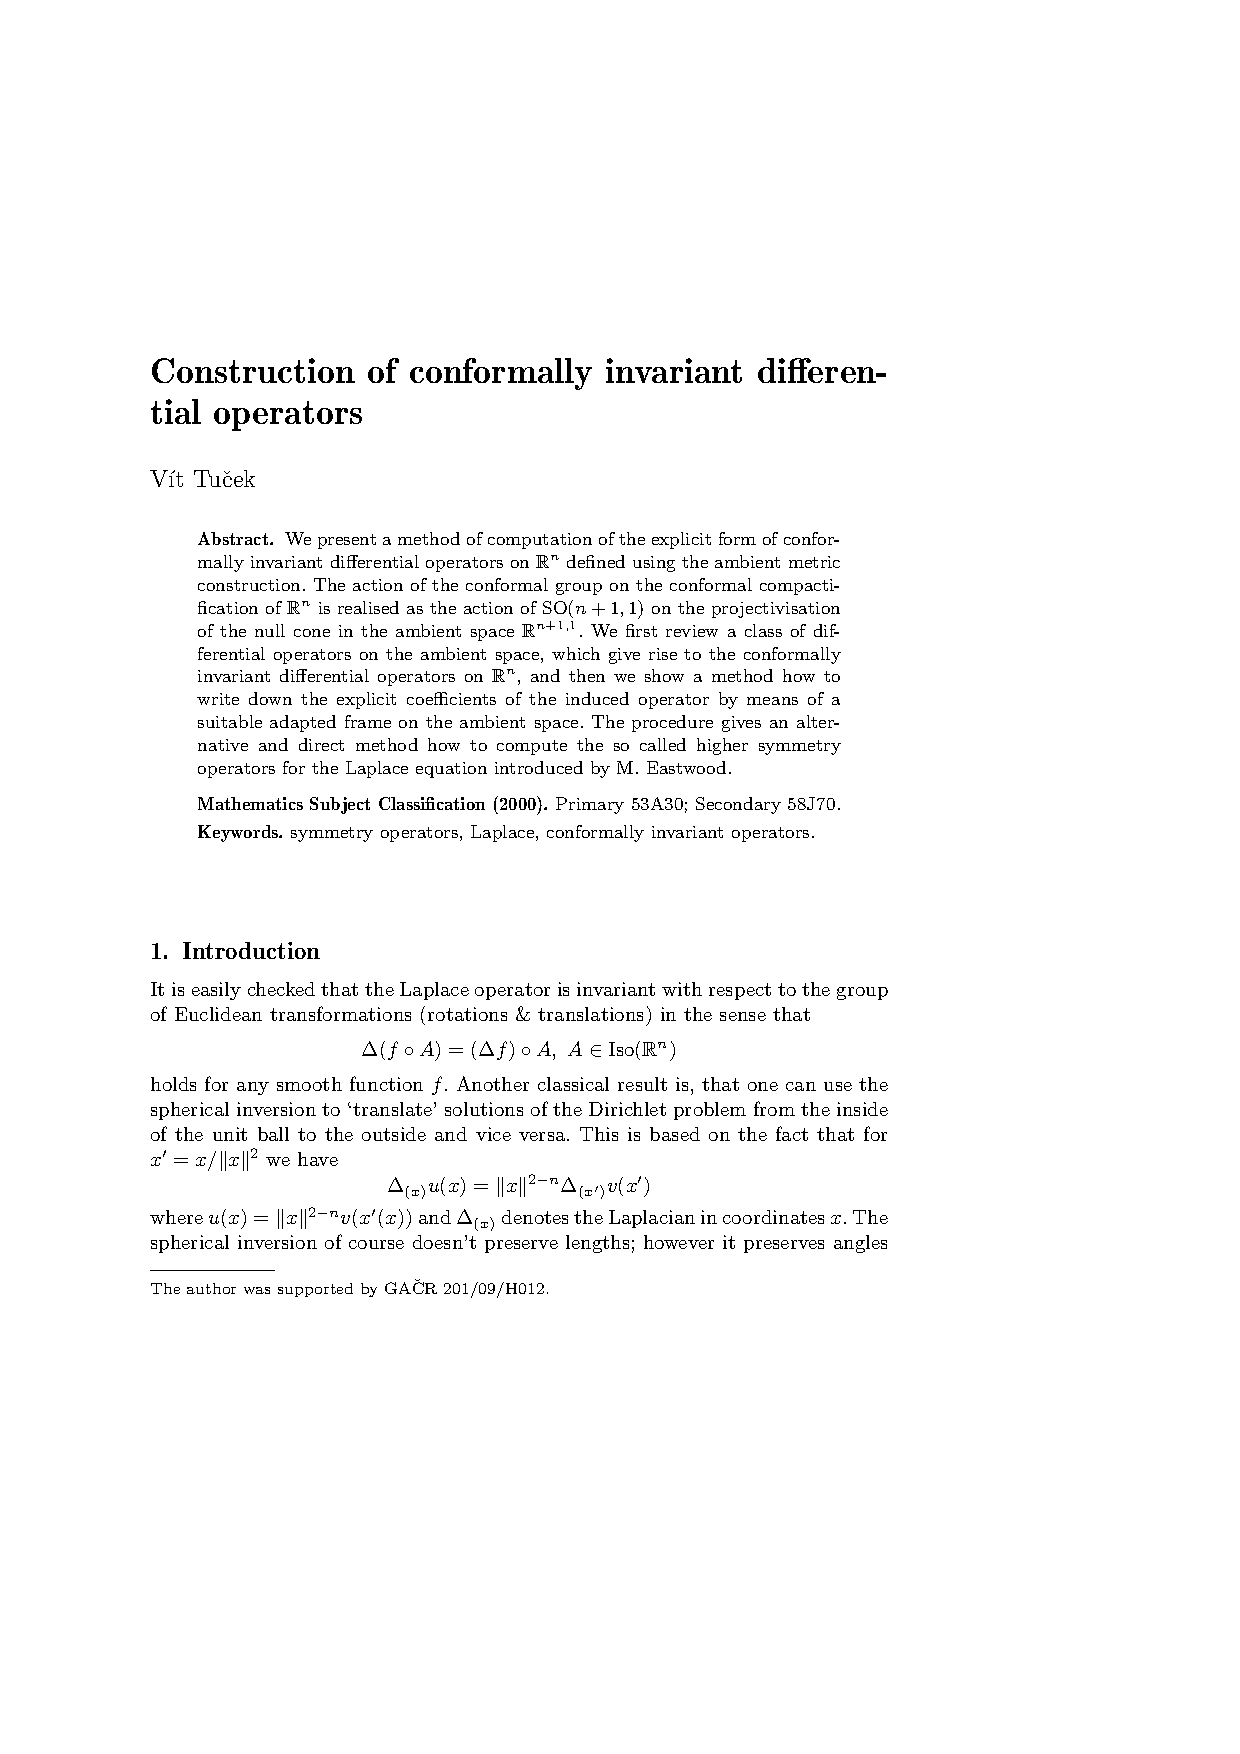
\includepdf[pages={-}]{articles/CoCIDO.pdf}
\includepdf[pages={2-}]{articles/CommentatMathUnivCarolRetro_52-2011-4_6.pdf}
\includepdf[pages={2-}]{articles/ArchMathRetro_048-2012-5_10.pdf}

\end{appendices}


%%% Tabulky v disertační práci, existují-li.
% \chapwithtoc{List of Tables}

%%% Použité zkratky v disertační práci, existují-li, včetně jejich vysvětlení.
% \chapwithtoc{List of Abbreviations}

%%% Přílohy k disertační práci, existují-li (různé dodatky jako výpisy programů,
%%% diagramy apod.). Každá příloha musí být alespoň jednou odkazována z vlastního
%%% textu práce. Přílohy se číslují.
% \chapwithtoc{Attachments}

\openright
\end{document}